\section{Topology}
    The following are notes from the appendix of Lee's Smooth Manifolds.
    \subsection{Basic Definitions}
        That is, topologies are closed to finite intersections, arbitrary
        unions, and contain both the empty set and the entire space.
        Elements of a topology are called the \textit{open} subsets of $X$.
        A closed subset is the complement of an open subset. That is,
        $C\subseteq{X}$ is closed if there exists an open set
        $\mathcal{U}\in\tau$ such that $C=X\setminus\mathcal{U}$.
        [Removed chaotic and distrete topology examples, and cont funcs]
        These are the two extreme examples of continuous functions. From
        analysis one talks about continuity by means of sequences. In an
        ideal world these two notions would coincide, but topological spaces
        can be quite pathalogical. One of our goals is to provide any
        hypothesis on a space so that we can allow our familiar notions from
        calculus to apply. We first define sequentially continuous functions
        and sequential spaces. To do so needs a notion of convergence. In
        analysis we say that $a_{n}\rightarrow{x}$ if for all
        $\varepsilon>0$ there is an $N\in\mathbb{N}$ such that for all
        $n\in\mathbb{N}$ with $n>N$ it is true that $|x-a_{n}|<\varepsilon$.
        One can picture this by drawing an interval of radius $\varepsilon$
        about the point $x$ and showing that eventually all of the points
        $a_{n}$ lie within this interval. To generalize to topological
        space, we replace intervals with open sets.
        \begin{fdefinition}{Convergent Sequence}{Convergent_Sequence}
            A convergent sequence in a topological space $\topspace{X}$ is a
            sequence $a:\mathbb{N}\rightarrow{X}$ such that there exists an
            $x\in{X}$ such that for all $\mathcal{U}\in\tau$ such that
            $x\in\mathcal{U}$ there exists an $N\in\mathbb{N}$ such that for
            all $n\in\mathbb{N}$ with $n>N$ it is true that
            $a_{n}\in\mathcal{U}$. We denote this by $a_{n}\rightarrow{x}$.
        \end{fdefinition}
        One of the firsts things one does in analysis when discussing
        sequences is prove that limits are unique. In topology this is
        false. Consider the chaotic topology on the real numbers
        $\nspace[]$. Then given any sequence
        $a:\mathbb{N}\rightarrow\nspace[]$ and any point $x\in\nspace[]$ it
        is true that $a_{n}\rightarrow{x}$. We can see this since there is
        only one non-empty subset, and that is the entirety of $\nspace[]$.
        And for all $n\in\mathbb{N}$ it is true that $a_{n}\in\nspace[]$ by
        the definition of $a$ being a sequence. Hence, $a_{n}$ converges to
        any point $x\in\nspace[]$ by the definition of convergence
        (Def.~\ref{def:Convergent_Sequence}). This doesn't mean that we've
        stumbled upon a poor definition of convergence, but rather that the
        trivial topology on a set is a rather poor topological space. To rid
        oneself of these oddities one must require spaces to have various
        separation properties. The most common to impose is the Hausdorff
        condition, and we will discuss this after defining sequentially
        continuous functions.
        \begin{fdefinition}{Sequentially Continuous Function}
                           {Sequentially_Continuous_Function}
            A sequentially continuous function from a topological space
            $\topspace[X]{X}$ to a topological space $\topspace[Y]{Y}$ is a
            function $f:X\rightarrow{Y}$ such that for every sequence
            $a:\mathbb{N}\rightarrow{X}$ and for every $x\in{X}$ such that
            $a_{n}\rightarrow{x}$, it is true that
            $f(a_{n})\rightarrow{f}(x)$.
        \end{fdefinition}
        We say for \textit{every} $x\in{X}$ since, as discussed before,
        limits may not be unique. As previsouly stated it is not necessarily
        true that sequentially continuous functions are continuous. We need
        to impose certain properties on the space to guarentee this. This
        converse, however, is true.
        \begin{theorem}
            \label{thm:Cont_is_Seq_Cont}%
            If $\topspace[X]{X}$ and $\topspace[Y]{Y}$ are topological
            spaces, and if $f:X\rightarrow{Y}$ is continuous, then it is
            sequentially continuous.
        \end{theorem}
        \begin{proof}
            For suppose not. Then there is a convergent sequence
            $a:\mathbb{N}\rightarrow{X}$ and a limt $x\in{X}$ of $a$ such
            that $a_{n}\rightarrow{x}$ but $f(a_{n})\not\rightarrow{f}(x)$
            (Def.~\ref{def:Sequentially_Continuous_Function}). But if
            $f(a_{n})\not\rightarrow{f}(x)$ then there exists an open subset
            $\mathcal{V}\in\tau_{Y}$ such that $f(x)\in\mathcal{V}$ and for
            all $N\in\mathbb{N}$ there exists an $n\in\mathbb{N}$ with
            $n>N$ and $f(a_{n})\notin\mathcal{V}$
            (Def.~\ref{def:Convergent_Sequence}). But if $f$ is continuous
            and $\mathcal{V}$ is open, then $f^{\minus{1}}[\mathcal{V}]$ is
            open (Def.~\ref{def:Continuous_Function}). But since
            $f(x)\in\mathcal{V}$ it is true that
            $x\in{f}^{\minus{1}}[\mathcal{V}]$. But $a_{n}\rightarrow{x}$
            and hence there is an $N\in\mathbb{N}$ such that for all
            $n\in\mathbb{N}$ with $n>N$ it is true that
            $a_{n}\in{f}^{\minus{1}}[\mathcal{V}]$
            (Def.~\ref{def:Convergent_Sequence}). But then for all $n>N$
            we have $f(a_{n})\in\mathcal{V}$, a contradiction.
        \end{proof}
        It would be nice to reverse this theorem. Now we could impose
        something strict like requiring $X$ to be a metric space, but should
        we ever encounter a non-metrizable space in the wild we'll have no
        tools to use. We seek a weak notion that is general enough to apply
        to just about every space one can imagine, but strong enough to
        ensure that sequentially continuous and continuous are equivalent.
        The concept we need is \textit{sequential} spaces. We'll build some
        point-set topology first, and then define sequential spaces. It may
        seem like unnecessary suspense, but sequential spaces are best
        defined when introducing their cousins \textit{first countable},
        \textit{second countable}, and \textit{separable} spaces.
        \begin{fdefinition}{Interior Point}{Interior_Point}
            An interior point of a subset $A\subseteq{X}$ of a topological
            space $\topspace{X}$ is a point $p\in{A}$ such that there exists
            an open set $\mathcal{U}\in\tau$ such that
            $\mathcal{U}\subseteq{A}$ and $p\in\mathcal{U}$.
        \end{fdefinition}
        \begin{example}
            If we let $I=[0,1]$, considered as a subset of $\nspace[]$, then
            every $x\in(0,1)$ is an interior point of $I$. To see this, let
            $\varepsilon>0$ be defined by:
            \begin{equation}
                \varepsilon=\minimum[\Big]{\frac{x}{2},\frac{1-x}{2}}
            \end{equation}
            since $x\in(0,1)$, $\varepsilon>0$. If we define
            $\mathcal{U}=(x-\varepsilon,x+\varepsilon)$, then
            $x\in\mathcal{U}$ and $\mathcal{U}\subseteq[0,1]$. Moreover,
            $\mathcal{U}$ is open and thus $x$ is an interior point of $I$.
        \end{example}
        Fig.~\ref{fig:Interior_Point_of_Set} shows two points $p$ and $q$ in
        a topological space $X$ and an arbitrary subset $A\subseteq{X}$. The
        point $p$ is an interior point of $A$ since we can surround $p$ with
        the blue open subset that lies entirely inside $A$. On the other
        hand, $q$ is \textit{not} an interior point of $A$ since every open
        subset that contains $q$ also contains points that are not in $A$.
        \begin{figure}[H]
            \centering
            \captionsetup{type=figure}
            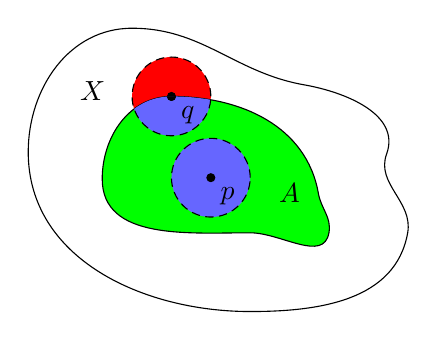
\begin{tikzpicture}
    \coordinate (p) at (-0.5, 0.7);
    \coordinate (q) at (120:2);
    \draw (0:2) to[out=80,  in=-110] (30:2)  to[out=70,  in=-10]  (70:2)
                to[out=170, in=0]    (120:3) to[out=180, in=90]   (160:3)
                to[out=-90, in=180]  (270:1) to[out=0,   in=-100] cycle;


    \draw[fill=red, densely dashed] (q) circle (5mm);
    \draw[fill=black] (q) circle (0.5mm);
    \node at (-2.0, 1.8) {$X$};
    \draw[fill=green] (0:1) to[out=80,  in=-80] (30:1)  to[out=100, in=0] (q)
                            to[out=180, in=90]  (160:2)
                            to[out=-90, in=180] (270:0) to[out=0,in=-100] cycle;

    \clip (0:1) to[out=80,  in=-80] (30:1)  to[out=100, in=0] (q)
                to[out=180, in=90]  (160:2)
                to[out=-90, in=180] (270:0) to[out=0,in=-100] cycle;
    \draw[densely dashed, fill=blue!60!white] (q) circle (5mm);
    \draw[densely dashed, fill=blue!60!white] (p) circle (5mm);
    \draw[fill=black] (p) circle (0.5mm);
    \draw[fill=black] (q) circle (0.5mm);
    \draw[fill=black] (q) circle (0.5mm);

    \node at ( 0.5, 0.5) {$A$};
    \node at (p) [below right] {$p$};
    \node at (q) [below right] {$q$};
\end{tikzpicture}
            \caption{Interior Point of a Set}
            \label{fig:Interior_Point_of_Set}
        \end{figure}
        \begin{example}
            Consider $\mathbb{Q}$ as a subset of $\nspace[]$, where
            $\nspace[]$ carries its usual metric topology. Then $\mathbb{Q}$
            has no interior points. For if $q\in\mathbb{Q}$, and if
            $\mathcal{U}$ is an open subset containing $q$, then there is an
            $\varepsilon>0$ such that
            $(q-\varepsilon,q+\varepsilon)\subseteq\mathcal{U}$. But then
            $(q-\varepsilon,q+\varepsilon)\subseteq\mathbb{Q}$. But for all
            $\varepsilon>0$, there is an irrational number $r$ such that
            $|q-r|<\varepsilon$, and thus
            $r\in(q-\varepsilon,q+\varepsilon)$ which is a contradiction
            since $(q-\varepsilon,q+\varepsilon)\subseteq\mathbb{Q}$. Hence,
            $\mathbb{Q}$ has no interior points.
        \end{example}
        \begin{example}
            For the same reasons, the irrational numbers
            $\mathbb{R}\setminus\mathbb{Q}$ also have no interior points.
        \end{example}
        \begin{fdefinition}{Interior of Set}{Interior_of_Set}
            The interior of a subset $A\subseteq{X}$ of a topological
            $\topspace{X}$, denoted $\interior[\tau]{A}$ is the set of all
            interior points of $A$. That is:
            \begin{equation*}
                \interior[\tau]{A}=\{\,p\in{X}\;|\;p
                    \textrm{ is an interior point of }A\,\}
            \end{equation*}
        \end{fdefinition}
        \begin{example}
            The previous examples allow us to compute the interior of a few
            sets quickly. If $I=[0,1]$, then every element of $(0,1)$ is an
            interior point. The endpoints 0 and 1 are not interior points
            since every $\varepsilon$ neighborhood must contain points
            outside of $[0,1]$. Thus, $\interior[{\nspace[]}]{I}=(0,1)$.
            Also, $\interior[{\nspace[]}]{\mathbb{Q}}=\emptyset$ and
            $\interior[{\nspace[]}]{\nspace[]\setminus\mathbb{Q}}=\emptyset$.
        \end{example}
        Borrowing from Fig.~\ref{fig:Interior_Point_of_Set}, we now present
        the interior of the set $A$, $\interior{A}$
        (Fig.~\ref{fig:Interior_of_Set}).
        \begin{figure}[H]
            \centering
            \captionsetup{type=figure}
            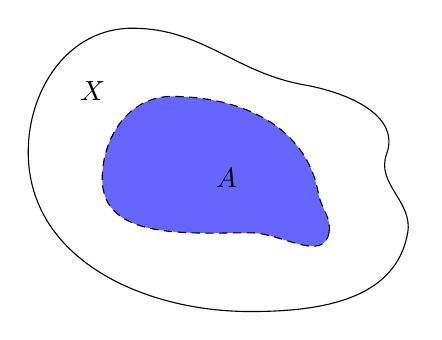
\begin{tikzpicture}
    \draw (0:2) to[out=80,  in=-110] (30:2)  to[out=70,  in=-10]  (70:2)
                to[out=170, in=0]    (120:3) to[out=180, in=90]   (160:3)
                to[out=-90, in=180]  (270:1) to[out=0,   in=-100] cycle;

    \draw[fill=blue!60!white, densely dashed]
        (0:1) to[out=80,  in=-80] (30:1)  to[out=100, in=0]   (120:2)
              to[out=180, in=90]  (160:2) to[out=-90, in=180] (270:0)
              to[out=0,in=-100] cycle;

    \node at (-0.3, 0.7) {$\interior{A}$};
    \node at (-2.0, 1.8) {$X$};
\end{tikzpicture}
            \caption{Interior of a Set}
            \label{fig:Interior_of_Set}
        \end{figure}
        \begin{theorem}
            \label{thm:Equiv_Def_Interior_of_Set}%
            If $\topspace{X}$ is a topological space, if
            $\tau_{A}$ is the set of all elements of $\tau$ that are subsets
            of in $A$, and if $\interior[\tau]{A}$ is the interior of $A$,
            then:
            \begin{equation}
                \interior[\tau]{A}=
                    \bigcup_{\mathcal{U}\in\tau_{A}}\mathcal{U}
            \end{equation}
        \end{theorem}
        \begin{proof}
            For if $p\in\interior[\tau]{A}$, then $p$ is an interior point
            of $A$ (Def.~\ref{def:Interior_of_Set}) and hence there is an
            open subset $\mathcal{U}\subseteq{A}$ such that
            $p\in\mathcal{U}$ (Def.~\ref{def:Interior_Point}). But then by
            hypothesis $\mathcal{U}\in\tau_{A}$, and hence
            $p\in\bigcup\tau_{A}$. Thus,
            $\interior[\tau]{A}\subseteq\bigcup\tau_{A}$. If
            $p\in\bigcup\tau_{A}$, then there is a $\mathcal{U}\in\tau_{A}$
            such that $p\in\mathcal{U}$. But by hypothesis if
            $\mathcal{U}\in\tau_{A}$, then $\mathcal{U}\subseteq{A}$, and
            hence $p$ is an interior point of $A$. Thus,
            $p\in\interior[\tau]{A}$. Therefore,
            $\interior[\tau]{A}=\bigcup\tau_{A}$.
        \end{proof}
        Thus, an equivalent formulation of the interior of a set is the
        union of all open sets that are contained in $A$.
        \begin{theorem}
            \label{thm:Interior_is_Smaller}%
            If $\topspace{X}$ is a topological space, and if
            $A\subseteq{X}$, then $\interior{A}\subseteq{A}$.
        \end{theorem}
        \begin{proof}
            For $\interior{A}=\bigcup\tau_{A}$, where $\tau_{A}\subseteq{A}$
            is the set of all element of $\tau$ that are contained in $A$
            (Thm.~\ref{thm:Equiv_Def_Interior_of_Set}). But then for all
            $\mathcal{U}\in\tau_{A}$, $\mathcal{U}\subseteq{A}$. Thus,
            $\bigcup\tau_{A}\subseteq{A}$, and therefore
            $\interior{A}\subseteq{A}$.
        \end{proof}
        \begin{theorem}
            \label{thm:Interior_is_Open}%
            If $\topspace{X}$ is a topological space, and if
            $A\subseteq{X}$, then $\interior{A}\in\tau$. That is, the
            interior of $A$ is open.
        \end{theorem}
        \begin{proof}
            For $\interior{A}=\bigcup\tau_{A}$, where
            $\tau_{A}\subseteq\tau$ is the set of all open subsets of $X$
            that are contained in $A$
            (Thm.~\ref{thm:Equiv_Def_Interior_of_Set}). But then
            $\interior{A}$ is the union of open subsets of $X$ and is hence
            open.
        \end{proof}
        \begin{theorem}
            \label{thm:Open_iff_Int_A_eq_A}%
            If $\topspace{X}$ is a topological space, and if
            $\mathcal{U}\subseteq{X}$, then $\mathcal{U}\in\tau$ if and only
            if $\interior{\mathcal{U}}=\mathcal{U}$.
        \end{theorem}
        \begin{proof}
            For if $\mathcal{U}\in\tau$, and if $\tau_{\mathcal{U}}$ is the
            set of all elements of $\tau$ that are subsets of $\mathcal{U}$,
            then $\mathcal{U}\in\tau_{\mathcal{U}}$ since
            $\mathcal{U}\subseteq\mathcal{U}$ and by hypothesis
            $\mathcal{U}\in\tau$. But
            $\interior{\mathcal{U}}=\bigcup\tau_{\mathcal{U}}$
            (Thm.~\ref{thm:Equiv_Def_Interior_of_Set}) and
            $\mathcal{U}\subseteq\bigcup\tau_{\mathcal{U}}$. But
            $\interior{\mathcal{U}}\subseteq\mathcal{U}$
            (Thm.~\ref{thm:Interior_is_Smaller}), and thus
            $\mathcal{U}=\interior{\mathcal{U}}$. In the other direction,
            since $\interior{\mathcal{U}}$ is open
            (Thm.~\ref{thm:Interior_is_Open}), if
            $\mathcal{U}=\interior{\mathcal{U}}$, then $\mathcal{U}$ is
            open.
        \end{proof}
        \begin{theorem}
            \label{thm:Interior_Preserves_Inclusion}%
            If $\topspace{X}$ is a topological space, if $A,B\subseteq{X}$,
            and if $A\subseteq{B}$, then
            $\interior{A}\subseteq\interior{B}$.
        \end{theorem}
        \begin{proof}
            For if $p\in\interior{A}$, then there is an open subset
            $\mathcal{U}\in\tau$ such that $p\in\mathcal{U}$ and
            $\mathcal{U}\subseteq{A}$ (Def.~\ref{def:Interior_of_Set}). But
            if $\mathcal{U}\subseteq{A}$ and $A\subseteq{B}$, then
            $\mathcal{U}\subseteq{B}$ and thus $p\in\interior{B}$
            (Def.~\ref{def:Interior_of_Set}).
        \end{proof}
        \begin{theorem}
            \label{thm:Open_Subset_of_A_is_Subset_of_Interior}%
            If $\topspace{X}$ is a topological space, if
            $\mathcal{U}\in\tau$ is open, if $A\subseteq{X}$, and if
            $\mathcal{U}\subseteq{A}$, then
            $\mathcal{U}\subseteq\interior{A}$.
        \end{theorem}
        \begin{proof}
            For if $\mathcal{U}\subseteq{A}$, then
            $\interior{\mathcal{U}}\subseteq\interior{A}$
            (Thm.~\ref{thm:Interior_Preserves_Inclusion}). But $\mathcal{U}$
            is open, and therefore $\interior{\mathcal{U}}=\mathcal{U}$
            (Thm.~\ref{thm:Open_iff_Int_A_eq_A}). Therefore
            $\mathcal{U}\subseteq\interior{A}$.
        \end{proof}
        \begin{theorem}
            \label{thm:Idempotence_of_Interior}
            If $\topspace{X}$ is a topological space, and if
            $A\subseteq{X}$, then:
            \begin{equation}
                \interior{\interior{A}}=\interior{A}
            \end{equation}
        \end{theorem}
        \begin{proof}
            For if $A\subseteq{X}$, then $\interior{A}$ is open
            (Thm.~\ref{thm:Interior_is_Open}). But if $\interior{A}$ is
            open, then $\interior{\interior{A}}=\interior{A}$
            (Thm.~\ref{thm:Open_iff_Int_A_eq_A}).
        \end{proof}
        \begin{theorem}
            \label{thm:Interior_of_Whole_Space}%
            If $\topspace{X}$ is a topological space, then $\interior{X}=X$.
        \end{theorem}
        \begin{proof}
            For if $\topspace{X}$ is a topological space, then $X\in\tau$.
            But if $X$ is open, then $\interior{X}=X$
            (Thm.~\ref{thm:Open_iff_Int_A_eq_A}).
        \end{proof}
        \begin{theorem}
            \label{thm:Interior_Preserves_Intersection}%
            If $\topspace{X}$ is a topological space, and if
            $A,B\subseteq{X}$, then:
            \begin{equation}
                \interior{A\cap{B}}=\interior{A}\cap\interior{B}
            \end{equation}
        \end{theorem}
        \begin{proof}
            For $\interior{A\cap{B}}=\bigcup\tau_{A\cap{B}}$, where
            $\tau_{A\cap{B}}\subseteq\tau$ is the set of all open subsets
            that are contained in $A\cap{B}$
            (Thm.~\ref{thm:Equiv_Def_Interior_of_Set}). Similarly,
            $\interior{A}=\bigcup\tau_{A}$ and $\interior{B}=\bigcup{B}$.
            But if $\mathcal{U}\in\tau_{A\cap{B}}$, then by definition
            $\mathcal{U}\in\tau$ and $\mathcal{U}\subseteq{A}\cap{B}$.
            But $A\cap{B}\subseteq{A}$, and hence $\mathcal{U}\subseteq{A}$.
            Hence, $\mathcal{U}\in\tau_{A}$ and similarly
            $\mathcal{U}\in\tau_{B}$. But then
            $\tau_{A\cap{B}}\subseteq\tau_{A}\cap\tau_{B}$, and therefore
            $\bigcup\tau_{A\cap{B}}\subseteq\bigcup\tau_{A}\cap\bigcup\tau_{B}$
            and thus $\interior{A\cap{B}}\subseteq\interior{A}\cap\interior{B}$.
            But if $x\in\interior{A}\cap\interior{B}$, then $x$ is an
            interior point of $A$ and an interior point of $B$
            (Def.~\ref{def:Interior_of_Set}) and there there exists
            $\mathcal{U}_{A},\mathcal{U}_{B}\in\tau$ such that
            $x\in\mathcal{U}_{A}$, $x\in\mathcal{U}_{B}$, and it is true
            that $\mathcal{U}_{A}\subseteq{A}$ and
            $\mathcal{U}_{B}\subseteq{B}$ (Def.~\ref{def:Interior_Point}).
            But then $\mathcal{U}_{A}\cap\mathcal{U}_{B}$ is an open subset,
            and $\mathcal{U}_{A}\cap\mathcal{U}_{B}\subseteq{A}\cap{B}$.
            Thus, $\mathcal{U}_{A}\cap\mathcal{U}_{B}\in\tau_{A\cap{B}}$,
            and thus $x\in\interior{A\cap{B}}$. Therefore
            $\interior{A\cap{B}}=\interior{A}\cap\interior{B}$.
        \end{proof}
        The theorems proved here can completely characterize topological
        spaces. Kuratowski famously did this with the notion of the
        \textit{closure} of a set, but interior works as well. That is, we
        define an \textit{interior operator} on a set as follows:
        \begin{fdefinition}{Interior Operator}{Interior_Operator}
            An interior operator on a set $X$ is a function
            $\sigma:\powset{X}\rightarrow\powset{X}$, where $\powset{X}$ is
            the power set of $X$, such that:
            \par
            \begin{subequations}
                \begin{minipage}[b]{0.49\textwidth}
                    \centering
                    \begin{align}
                        \label{eqn:Int_Op_Inclusion}%
                        \sigma(A)&\subseteq{A}\tag{1}\\
                        \label{eqn:Int_Op_Idemp}%
                        \sigma\big(\sigma(A)\big)&=\sigma(A)\tag{2}
                    \end{align}
                \end{minipage}
                \hfill
                \begin{minipage}[b]{0.49\textwidth}
                    \centering
                    \begin{align}
                        \label{eqn:Int_Op_Intersect}%
                        \sigma(A\cap{B})&=\sigma(A)\cap\sigma(B)\tag{3}\\
                        \label{eqn:Int_Op_Preserve_X}%
                        \sigma(X)&=X\tag{4}
                    \end{align}
                \end{minipage}
            \end{subequations}
            \par\vspace{2.5ex}
        \end{fdefinition}
        Eqn.~\ref{eqn:Int_Op_Intersect} has an equivalent formulation called
        \textit{isotonicity}. We will need this later.
        \begin{theorem}
            \label{thm:Int_Op_Isoton}%
            If $X$ is a set, if $\sigma:\powset{X}\rightarrow\powset{X}$ is
            an interior operator, if $A,B\subseteq{X}$, and if
            $A\subseteq{B}$, then $\sigma(A)\subseteq\sigma(B)$.
        \end{theorem}
        \begin{proof}
            For if $A\subseteq{B}$, then $A\cap{B}=A$, and therefore
            $\sigma(A)=\sigma(A\cap{B})$. But
            $\sigma(A\cap{B})=\sigma(A)\cap\sigma(B)$
            (Def.~\ref{def:Interior_Operator}
            Eqn.~\ref{eqn:Int_Op_Intersect}). Therefore,
            $\sigma(A)\subseteq\sigma(B)$.
        \end{proof}
        A topology gives a unique interior operator that preserves the open
        sets, and an interior operator gives a unique topology. We still
        need the notion of \textit{morphism}, and in the ordinary study of
        topology we have continuous functions. The following theorem gives
        an equivalent definition of continuity in terms of interior.
        \begin{ftheorem}{Kuratowski's Interior Theorem}
                        {Kuratowski_Interior_Thm}
            If $\topspace[X]{X}$ and $\topspace[Y]{Y}$ are topological
            spaces, and if $f:X\rightarrow{Y}$ is a function, then $f$ is
            continuous if and only if for all $B\subseteq{Y}$ it is true
            that:
            \begin{equation*}
                f^{\minus{1}}[\interior[Y]{B}]\subseteq
                    \interior[X]{f^{\minus{1}}[B]}
            \end{equation*}
        \end{ftheorem}
        \begin{bproof}
            For suppose $f$ is continuous. But if $B\subseteq{Y}$, then
            $\interior[Y]{B}$ is an open subset of $Y$
            (Thm.~\ref{thm:Interior_is_Open}). But if $\interior[Y]{B}$ is
            open and $f$ is continuous, then
            $f^{\minus{1}}[\interior[Y]{B}]$ is an open subset of $X$.
            Moreover, $\interior[Y]{B}\subseteq{B}$
            (Thm.~\ref{thm:Interior_is_Smaller}) and therefore
            $f^{\minus{1}}[\interior[Y]{B}]\subseteq{f}^{\minus{1}}[B]$. But
            then $f^{\minus{1}}[\interior[Y]{B}]$ is an open subset
            contained in $f^{\minus{1}}[B]$, and therefore
            $f^{\minus{1}}[\interior[Y]{B}]\subseteq%
            \interior[X]{f^{\minus{1}}[B]}$
            (Thm.~\ref{thm:Open_Subset_of_A_is_Subset_of_Interior}). In the
            other direction, suppose $f$ preserves the interior. If $f$ is
            not continuous, then there is an open subset
            $\mathcal{V}\in\tau_{Y}$ such that $f^{\minus{1}}[\mathcal{V}]$
            is not an open subset of $X$. But if $\mathcal{V}$ is open, then
            $\interior[Y]{\mathcal{V}}=\mathcal{V}$
            (Thm.~\ref{thm:Open_iff_Int_A_eq_A}). But then by hypothesis:
            \begin{equation}
                f^{\minus{1}}[\mathcal{V}]\subseteq
                \interior[X]{f^{\minus{1}}[\mathcal{V}]}
            \end{equation}
            But $\interior[X]{f^{\minus{1}}[\mathcal{V}]}\subseteq%
            f^{\minus{1}}[\mathcal{V}]$
            (Thm.~\ref{thm:Interior_is_Smaller}), and therefore
            $f^{\minus{1}}[\mathcal{V}]=%
             \interior[X]{f^{\minus{1}}[\mathcal{V}]}$. But
            $\interior[X]{f^{\minus{1}}[\mathcal{V}]}$ is open
            (Thm.~\ref{thm:Interior_is_Open}), and thus
            $f^{\minus{1}}[\mathcal{V}]$ is open, a contradiction.
            Therefore, $f$ is continuous.
        \end{bproof}
        With this, we now prove our claim that the interior operator is an
        equivalent formulation of topology. Def.~\ref{def:Interior_Operator}
        gives a complete algebraic axiomization of the notion of topologies
        on a set. One may be tempted to think that these four equations
        satisfy a \textit{unique} interior operator
        (that is, $\sigma=\textrm{Int}_{\tau}$), but there's a different
        distinct interior operator for every topology $\tau$ on a set $X$.
        Thus, to prove any form of uniqueness we must greatly strengthen
        Eqn.~\ref{eqn:Int_Op_Preserve_X} so that $\sigma$ pertains to a
        single topology. We do this by requiring the
        $\sigma(\mathcal{U})=\mathcal{U}$ if and only if $\mathcal{U}$ is
        open. This new requirement gives us a bijection between interior
        operators and topologies.
        \begin{ftheorem}{Interior Operator of a Topological Space}
                        {Interior_Operator_of_a_Topological_Space}
            If $\topspace{X}$ is a topological space, if
            $\sigma:\powset{X}\rightarrow\powset{X}$ is an interior operator
            on $X$, and if $\mathcal{U}\in\tau$ if and only if
            $\sigma(\mathcal{U})=\mathcal{U}$, then
            $\sigma(A)=\interior{A}$.
        \end{ftheorem}
        \begin{bproof}
            For suppose not. Then there is an $A\in\powset{X}$ such that
            $\sigma(A)\ne\interior{A}$. But then there either
            $\sigma(A)\nsubseteq\interior{A}$ or
            $\interior{A}\nsubseteq{A}$. But $\interior{A}$ is open
            (Thm.~\ref{thm:Interior_is_Open}) so by hypothesis
            $\sigma(\interior{A})=\interior{A}$. But
            $\interior{A}\subseteq{A}$ (Thm.~\ref{thm:Interior_is_Smaller})
            and therefore $\interior{A}=A\cap\interior{A}$. But
            $\sigma(A\cap\interior{A})=\sigma(A)\cap\sigma(\interior{A})$
            (Def.~\ref{def:Interior_Operator}
            Eqn.~\ref{eqn:Int_Op_Intersect}) and
            $\sigma(A)\cap\sigma(\interior{A})=\sigma(A)\cap\interior{A}$.
            Therefore by the transitivity of equality we obtain
            $\interior{A}=\sigma(A)\cap\interior{A}$, and therefore
            $\interior{A}\subseteq\sigma(A)$. But
            $\sigma(\sigma(A))=\sigma(A)$ (Def.~\ref{def:Interior_Operator}
            Eqn.~\ref{eqn:Int_Op_Idemp}), and thus by hypothesis $\sigma(A)$
            is open. But since $\sigma(A)\subseteq{A}$
            (Def.~\ref{def:Interior_Operator}
            Eqn.~\ref{eqn:Int_Op_Inclusion}), if $\sigma(A)$ is open, then
            $\sigma(A)\subseteq\interior{A}$
            (Thm.~\ref{thm:Open_Subset_of_A_is_Subset_of_Interior}).
            Therefore $\sigma(A)=\interior{A}$, a contradiction. Hence, for
            all $A\subseteq{X}$ it is true that $\sigma(A)=\interior{A}$.
        \end{bproof}
        We now define the induced topology of an interior operator, and show
        that it is indeed a topology.
        \begin{fdefinition}{Induced Topology of an Interior Operator}
                           {Induced_Topology_of_an_Interior_Operator}
            The induced topology of and interior operator
            $\sigma:\powset{X}\rightarrow\powset{X}$ on a set $X$ is the set
            of all $\mathcal{U}\in\powset{X}$ such that
            $\sigma(\mathcal{U})=\mathcal{U}$. That is:
            \begin{equation*}
                \tau_{\sigma}=\big\{\,\mathcal{U}\in\powset{X}\;|\;
                    \sigma(\mathcal{U})=\mathcal{U}\,\}
            \end{equation*}
        \end{fdefinition}
        Just because we're calling this thing a topology doesn't mean it is.
        We now prove that the induced topology of an interior operator is
        indeed a topology, and thus $\topspace[\sigma]{X}$ is a topological
        space.
        \begin{theorem}
            \label{thm:Top_Induced_by_Int_Op_is_Top}%
            If $X$ is a set, if $\sigma:\powset{X}\rightarrow\powset{X}$ is
            an interior operator on $X$, and if $\tau_{\sigma}$ is the
            induced topology of $\sigma$, then $\tau_{\sigma}$ is a topology
            on $X$.
        \end{theorem}
        \begin{proof}
            For if $\sigma$ is an interior operator, then $\sigma(X)=X$
            (Def.~\ref{def:Interior_Operator}
            Eqn.~\ref{eqn:Int_Op_Preserve_X}) and thus $X\in\tau_{\sigma}$.
            Moreover, since $\sigma(\emptyset)\subseteq\emptyset$
            (Def.~\ref{def:Interior_Operator}
            Eqn.~\ref{eqn:Int_Op_Inclusion}), it is therefore true that
            $\emptyset\in\tau_{\sigma}$. If
            $\mathcal{U},\mathcal{V}\in\tau_{\sigma}$, then:
            \begin{align}
                \sigma(\mathcal{U}\cap\mathcal{V})
                    &=\sigma(\mathcal{U})\cap\sigma(\mathcal{V})
                    \tag{Def.~\ref{def:Interior_Operator}
                        Eqn.~\ref{eqn:Int_Op_Intersect}}\\
                    &=\mathcal{U}\cap\mathcal{V}
                    \tag{Hypothesis}
            \end{align}
            and hence $\mathcal{U}\cap\mathcal{V}\in\tau_{\sigma}$. Lastly,
            if $\mathcal{O}\subseteq\tau_{\sigma}$, then:
            \begin{equation}
                \sigma\Big(
                    \bigcup_{\mathcal{U}\in\mathcal{O}}\mathcal{U}
                \Big)
                \subseteq\bigcup_{\mathcal{U}\in\mathcal{O}}\mathcal{U}
                    \tag{Def.~\ref{def:Interior_Operator}
                        Eqn.~\ref{eqn:Int_Op_Inclusion}}
            \end{equation}
            But for all $\mathcal{U}\in\mathcal{O}$,
            $\mathcal{U}\subseteq\bigcup\mathcal{O}$ and therefore
            $\sigma(\mathcal{U})\subseteq\sigma(\bigcup\mathcal{O})$
            (Thm.~\ref{thm:Int_Op_Isoton}). But then:
            \begin{equation}
                \bigcup_{\mathcal{U}\in\mathcal{O}}
                    \sigma(\mathcal{U})\subseteq
                \sigma\Big(\bigcup_{\mathcal{U}\in\mathcal{O}}
                    \mathcal{U}\Big)
            \end{equation}
            By hypothesis $\sigma(\mathcal{U})=\mathcal{U}$, and so
            $\bigcup\mathcal{O}\subseteq\sigma(\bigcup\mathcal{O})$. But
            $\sigma(\bigcup\mathcal{O})\subseteq\bigcup\mathcal{O}$,
            and therefore $\sigma(\bigcup\mathcal{O})=\bigcup\mathcal{O}$.
            Hence, $\bigcup\mathcal{O}\in\tau_{\sigma}$ and $\tau_{\sigma}$
            is a topology on $X$.
        \end{proof}
        There's a related notion called \textit{exterior}. Like the
        interior, we define the exterior in terms of exterior points.
        \begin{fdefinition}{Exterior Point}{Exterior_Point}
            An exterior point of a subset $A\subseteq{X}$ of a topological
            spacec $\topspace{X}$ is a point $p\in{X}\setminus{A}$ such that
            there exists an open set $\mathcal{U}\in\tau$ with
            $\mathcal{U}\subseteq{X}\setminus{A}$ and $p\in\mathcal{U}$.
        \end{fdefinition}
        As one might expect from the definition, there's nothing new here
        and exterior points can be related to interior points be means of
        complement.
        \begin{figure}[H]
            \centering
            \captionsetup{type=figure}
            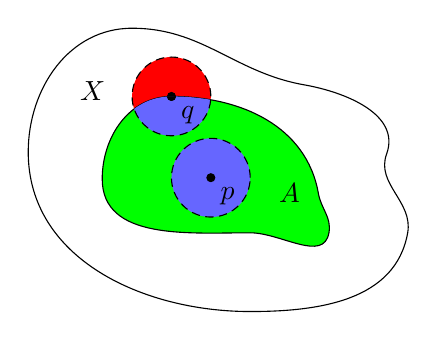
\begin{tikzpicture}
    \coordinate (p) at (-0.5, 0.7);
    \coordinate (q) at (120:2);
    \draw (0:2) to[out=80,  in=-110] (30:2)  to[out=70,  in=-10]  (70:2)
                to[out=170, in=0]    (120:3) to[out=180, in=90]   (160:3)
                to[out=-90, in=180]  (270:1) to[out=0,   in=-100] cycle;


    \draw[fill=red, densely dashed] (q) circle (5mm);
    \draw[fill=black] (q) circle (0.5mm);
    \node at (-2.0, 1.8) {$X$};
    \draw[fill=green] (0:1) to[out=80,  in=-80] (30:1)  to[out=100, in=0] (q)
                            to[out=180, in=90]  (160:2)
                            to[out=-90, in=180] (270:0) to[out=0,in=-100] cycle;

    \clip (0:1) to[out=80,  in=-80] (30:1)  to[out=100, in=0] (q)
                to[out=180, in=90]  (160:2)
                to[out=-90, in=180] (270:0) to[out=0,in=-100] cycle;
    \draw[densely dashed, fill=blue!60!white] (q) circle (5mm);
    \draw[densely dashed, fill=blue!60!white] (p) circle (5mm);
    \draw[fill=black] (p) circle (0.5mm);
    \draw[fill=black] (q) circle (0.5mm);
    \draw[fill=black] (q) circle (0.5mm);

    \node at ( 0.5, 0.5) {$A$};
    \node at (p) [below right] {$p$};
    \node at (q) [below right] {$q$};
\end{tikzpicture}
            \caption{Exterior Point of a Set}
            \label{fig:Exterior_Points}
        \end{figure}
        \begin{theorem}
            \label{thm:Equiv_Def_Exterior_Point_of_Set}%
            If $\topspace{X}$ is a topological space, if $A\subseteq{X}$,
            and if $p\in{X}$, then $p$ is an exterior point of $A$ if and
            only if it is an interior point of $X\setminus{A}$.
        \end{theorem}
        \begin{proof}
            For if $p$ is an exterior point of $A$, then there is an open
            subset $\mathcal{U}\in\tau$ such that
            $\mathcal{U}\subseteq{X}\setminus{A}$ and $p\in\mathcal{U}$
            (Def.~\ref{def:Exterior_Point}). But then $p\in{X}\setminus{A}$
            and there exists an open subset $\mathcal{U}\in\tau$ such that
            $\mathcal{U}\subseteq{X}\setminus{A}$ and hence $p$ is an
            interior point of $X\setminus{A}$
            (Def.~\ref{def:Interior_Point}). If
            $p\in\interior{X\setminus{A}}$, then there is an open subset
            $\mathcal{U}\in\tau$ such that $p\in\mathcal{U}$ and
            $\mathcal{U}\subseteq{X}\setminus{A}$. But then $p$ is an
            exterior point of $A$ (Def.~\ref{def:Exterior_Point}).
        \end{proof}
        \begin{example}
            Using Thm.~\ref{thm:Equiv_Def_Exterior_Point_of_Set} we have
            that every point in $(\minus\infty,0)\cup(1,\infty)$ is an
            exterior point of the set $I=[0,1]$.
        \end{example}
        \begin{fdefinition}{Exterior of a Set}{Exterior_of_a_Set}
            The exterior of a subset $A\subseteq{X}$ in a topological space
            $\topspace{X}$, denoted $\exterior[\tau]{A}$, is the set of all
            exterior points of $A$. That is:
            \begin{equation*}
                \exterior{A}=\{\,p\in{X}\;|\;
                    p\textrm{ is an exterior point of }X\,\}
            \end{equation*}
        \end{fdefinition}
        \begin{theorem}
            \label{thm:Equiv_Def_of_Exterior_of_Set}%
            If $\topspace{X}$ is a topological space, and if
            $A\subseteq{X}$, then:
            \begin{equation}
                \exterior{A}=\interior{X\setminus{A}}
            \end{equation}
        \end{theorem}
        \begin{proof}
            For if $p\in\exterior{A}$ if and only if $p$ is an exterior
            point of $A$ (Def.~\ref{def:Exterior_of_a_Set}). But $p$ is an
            exterior point of $A$ if and only if it is an interior point of
            $X\setminus{A}$ (Thm.~\ref{thm:Equiv_Def_Exterior_Point_of_Set}).
            But $p\in\interior{X\setminus{A}}$ if and only if
            $p\in\interior{X\setminus{A}}$. Therefore, we have that
            $\exterior{A}=\interior{X\setminus{A}}$.
        \end{proof}
        \begin{example}
            When we examined the interior of the rationals and irrationals
            we noted that both were empty, and hence both
            $\exterior[{\nspace[]}]{\mathbb{Q}}$ and
            $\exterior[{\nspace[]}]{\nspace[]\setminus\mathbb{Q}}$ are
            empty. That is, $\mathbb{Q}$ has empty interior and empty
            exterior, even though $\mathbb{Q}$ is dense in $\nspace[]$,
            which is quite paradoxical.
        \end{example}
        This example shows that the exterior of a set is not just the
        complement. There are three parts to a set: Interior, exterior, and
        boundary. This shows that, whatever boundary is defined to be, the
        boundary of $\mathbb{Q}$ is the entirety of $\mathbb{R}$, which
        again may be at odds with intuition.
        \begin{figure}[H]
            \centering
            \captionsetup{type=figure}
            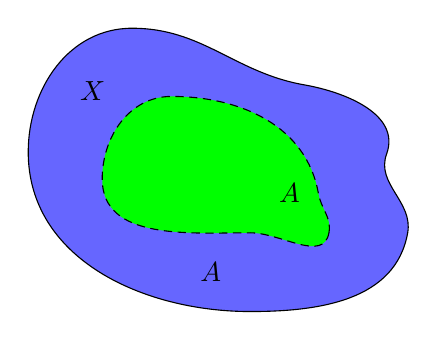
\begin{tikzpicture}
    \draw[fill=blue!60!white] (0:2) to[out=80,  in=-110] (30:2)  to[out=70,  in=-10]  (70:2)
                to[out=170, in=0]    (120:3) to[out=180, in=90]   (160:3)
                to[out=-90, in=180]  (270:1) to[out=0,   in=-100] cycle;

    \draw[fill=green, densely dashed]
        (0:1) to[out=80,  in=-80] (30:1)  to[out=100, in=0]   (120:2)
              to[out=180, in=90]  (160:2) to[out=-90, in=180] (270:0)
              to[out=0,in=-100] cycle;

    \node at (-0.5, -0.5) {$\exterior{A}$};
    \node at (-2.0, 1.8) {$X$};
    \node at ( 0.5, 0.5) {$A$};
\end{tikzpicture}
            \caption{Exterior a Set}
            \label{fig:Exterior_of_Set}
        \end{figure}
        \begin{theorem}
            \label{thm:Alt_Equiv_Def_Exterior_of_Set}%
            If $\topspace{X}$ is a topological space, if $A\subseteq{X}$, if
            $\tau_{A^{C}}$ is the set of all open subsets contained in
            $X\setminus{A}$, then:
            \begin{equation}
                \exterior{A}=\bigcup_{\mathcal{U}\in\tau_{A}^{C}}\mathcal{U}
            \end{equation}
        \end{theorem}
        \begin{proof}
            For $\exterior{A}=\interior{X\setminus{A}}$
            (Thm.~\ref{thm:Equiv_Def_of_Exterior_of_Set}). But
            $\interior{X\setminus{A}}=\bigcup\tau_{A^{C}}$
            (Thm.~\ref{thm:Equiv_Def_Interior_of_Set}) and therefore
            $\exterior{A}=\bigcup\tau_{A^{C}}$.
        \end{proof}
        We attempt to define boundary in an intuitive manner. To do this
        needs the notion of \textit{closure}, which is somewhat the
        \textit{dual} concept of interior. Kuratowski's interests were in
        the closure axioms that could be used to define topological spaces,
        and indeed in his two volume treatise on topology he takes as the
        definition of a topological space a set $X$ with a closure operator
        $\sigma$. Like interior, closure is defined in terms of closure
        points.
        \begin{fdefinition}{Point of Closure}{Point_of_Closure}
            A point of closure of a subset $A\subseteq{X}$ in a topological
            space $\topspace{X}$ is a point $p\in{X}$ such that for every
            open subset $\mathcal{U}\in\tau$ such that $p\in\mathcal{U}$ it
            is true that $\mathcal{U}\cap{A}\ne\emptyset$.
        \end{fdefinition}
        \begin{example}
            In the setting of metric spaces, points of closure of a subset
            $A\subseteq{X}$ are points in $X$ that can be approximated
            arbitrarily well by points in $A$. That is, the points $x\in{X}$
            such that for any $\varepsilon>0$ one can find and $a\in{A}$
            such that the distance between $a$ and $x$ is less than
            $\varepsilon$. In other words, one can find a sequence
            $a:\mathbb{N}\rightarrow{A}$ such that $a_{n}\rightarrow{x}$.
            For example, $\pi\in\mathbb{R}$ is a point of closure of the
            rationals $\mathbb{Q}$. We can form the sequence 3, 3.1, 3.14,
            3.141, and so on. Using the actual definition of points of
            closure, given any open set about $\pi$ there are rational
            numbers contained in this set.
        \end{example}
        \begin{fdefinition}{Closure}{Closure}
            The closure of a subset $A\subseteq{X}$ in a topological space
            $\topspace{X}$ is the set:
            \begin{equation*}
                \closure{X}=\{\,x\in{X}\;|\;
                    x\textrm{ is a closure point of }A\,\}
            \end{equation*}
        \end{fdefinition}
        \begin{example}
            Since every irrational number can be approximated arbitrarily
            well by rational numbers, we can see that the closure of the
            rationals is all of the reals. That is,
            $\closure{\mathbb{Q}}=\nspace[]$.
        \end{example}
        \begin{example}
            As a similar example the closure of the irrationals is all of
            $\nspace[]$.
        \end{example}
        Much like the interior of a set, many of the \textit{dual} theorems
        about closures can be proved.
        \begin{theorem}
            \label{thm:Alt_Equiv_Def_Closure_of_Set}%
            If $\topspace{X}$ is a topological space, if $\tau_{A^{C}}$ is
            the set of all closed subsets that contain $A$, then:
            \begin{equation}
                \closure{A}=\bigcap_{\mathcal{C}\in\tau_{A^{C}}}\mathcal{C}
            \end{equation}
        \end{theorem}
        \begin{proof}
            For suppose not. If $x\in\closure{A}$ and if
            $x\notin\bigcap\tau_{A^{C}}$, then there is a closed subset
            $\mathcal{C}\subseteq{X}$ such that $A\subseteq\mathcal{C}$ and
            $x\notin\mathcal{C}$. But then $x\in{X}\setminus\mathcal{C}$ and
            $X\setminus\mathcal{C}$ is the complement of a closed set, and
            is thus open. But then $X\setminus\mathcal{C}$ is an open subset
            of $X$ such that contains $x$ and has empty intersection with
            $A$, a contradiction since $x\in\closure{A}$ and hence $x$ is a
            point of closure (Def.~\ref{def:Closure}). Therefore,
            $\closure{A}\subseteq\bigcap\tau_{A^{C}}$. Next, suppose
            $x\in\bigcap\tau_{A^{C}}$ and $x\notin\closure{A}$. But if
            $x\notin\closure{A}$, then $x$ is not a point of closure
            (Def.~\ref{def:Closure}) and hence there is an open subset
            $\mathcal{U}\in\tau$ such that $x\in\mathcal{U}$ and
            $\mathcal{U}\cap{A}=\emptyset$
            (Def.~\ref{def:Point_of_Closure}). But then
            $A\subseteq{X}\setminus\mathcal{U}$ and
            $x\notin{X}\setminus\mathcal{U}$. But $X\setminus\mathcal{U}$
            is closed, and hence is an element of $\tau_{A^{C}}$. But
            $x\in\bigcap\tau_{A^{C}}$, a contradiction. Therefore, we have
            equality.
        \end{proof}
        \begin{theorem}
            \label{thm:Closure_is_Bigger}%
            If $\topspace{X}$ is a topological space, and if
            $A\subseteq{X}$, then $A\subseteq\closure{A}$.
        \end{theorem}
        \begin{proof}
            For $\closure{A}=\bigcap\tau_{A^{C}}$
            (Thm.~\ref{thm:Alt_Equiv_Def_Closure_of_Set}), where
            $\tau_{A^{C}}$ is the set of all closed subsets that contain
            $A$. But then for all $\mathcal{C}\in\tau_{A^{C}}$ we have
            $A\subseteq\mathcal{C}$ and thus
            $A\subseteq\bigcap\tau_{A^{C}}$.
        \end{proof}
        \begin{theorem}
            \label{thm:Closure_is_Closed}%
            If $\topspace{X}$ is a topological space, and if
            $A\subseteq{X}$, then $\closure{A}$ is closed.
        \end{theorem}
        \begin{proof}
            For $\closure{A}=\bigcap\tau_{A^{C}}$, where $\tau_{A^{C}}$ is
            the set of all closed subsets that contain $A$
            (Thm.~\ref{thm:Alt_Equiv_Def_Closure_of_Set}). But then
            $\closure{A}$ is the intersection of closed sets, and is thus
            closed.
        \end{proof}
        \begin{theorem}
            \label{thm:Closed_iff_Cl_A_Eq_A}%
            If $\topspace{X}$ is a topological space, and if
            $A\subseteq{X}$, then $A$ is closed if and only if
            $\closure{A}=A$.
        \end{theorem}
        \begin{proof}
            For if $\closure{A}$ is closed
            (Thm.~\ref{thm:Closure_is_Closed}), and hence if
            $A=\closure{A}$, then $A$ is closed. If $A$ is closed, then
            $A\in\tau_{A^{C}}$ where $\tau_{A^{C}}$ is the set of all closed
            subsets of $X$ that contain $A$. But
            $\closure{A}=\bigcap\tau_{A^{C}}$
            (Thm.~\ref{thm:Alt_Equiv_Def_Closure_of_Set}) and
            $\bigcap\tau_{A^{C}}\subseteq{A}$, and hence
            $\closure{A}\subseteq{A}$. But $A\subseteq\closure{A}$
            (Thm.~\ref{thm:Closure_is_Bigger}) and thus $A=\closure{A}$.
        \end{proof}
        \begin{theorem}
            \label{thm:Closure_Preserves_Inclusion}%
            If $\topspace{X}$ is a topological space, if $A,B\subseteq{X}$,
            and if $A\subseteq{B}$, then $\closure{A}\subseteq\closure{B}$.
        \end{theorem}
        \begin{proof}
            For if $x\in\closure{A}$, then $x$ is a point of closure of $A$
            (Def.~\ref{def:Closure}). But then for all $\mathcal{U}\in\tau$
            such that $x\in\mathcal{U}$, $A\cap\mathcal{U}$ is non-empty
            (Def.~\ref{def:Point_of_Closure}). But $A\subseteq{B}$, and
            hence $B\cap\mathcal{U}\ne\emptyset$. Thus, $x\in\closure{A}$.
        \end{proof}
        \begin{theorem}
            \ref{thm:Closed_Superset_of_A_is_Superset_of_Closure}%
            If $\topspace{X}$ is a topological space, if $A\subseteq{X}$,
            if $\mathcal{C}$ is closed, and if $A\subseteq\mathcal{C}$,
            then $\closure{A}\subseteq\mathcal{C}$.
        \end{theorem}
        \begin{proof}
            For if $A\subseteq\mathcal{C}$, then
            $\closure{\mathcal{C}}\subseteq\closure{\mathcal{C}}$
            (Thm.~\ref{thm:Closure_Preserves_Inclusion}). But $\mathcal{C}$
            is closed, and thus $\closure{\mathcal{C}}=\mathcal{C}$
            (Thm.~\ref{thm:Closed_iff_Cl_A_Eq_A}). Therefore,
            $\closure{A}\subseteq\mathcal{C}$.
        \end{proof}
        \begin{theorem}
            \label{thm:Idempotence_of_Closure}%
            If $\topspace{X}$ is a topological space, and if
            $A\subseteq{X}$, then:
            \begin{equation}
                \closure{\closure{A}}=\closure{A}
            \end{equation}
        \end{theorem}
        \begin{proof}
            For if $A\subseteq{X}$, then $\closure{A}$ is a closed subset
            (Thm.~\ref{thm:Closure_is_Closed}). But if $\closure{A}$ is
            closed, then $\closure{\closure{A}}=\closure{A}$
            (Thm.~\ref{thm:Closed_iff_Cl_A_Eq_A}).
        \end{proof}
        \begin{theorem}
            \label{thm:Closure_of_Whole_Space}%
            If $\topspace{X}$ is a topological space, then $\closure{X}=X$.
        \end{theorem}
        \begin{proof}
            For $X$ is closed, and hence $\closure{X}=X$
            (Thm.~\ref{thm:Closed_iff_Cl_A_Eq_A}).
        \end{proof}
        \begin{theorem}
            \label{thm:Closure_Preserves_Union}%
            If $\topspace{X}$ is a topological space, and if
            $A,B\subseteq{X}$, then:
            \begin{equation}
                \closure{A\cup{B}}=\closure{A}\cup\closure{B}
            \end{equation}
        \end{theorem}
        \begin{proof}
            For if $x\in\closure{A\cup{B}}$, then $x$ is a point of closure
            of $A\cup{B}$ (Def.~\ref{def:Closure}) and hence for all
            $\mathcal{U}\in\tau$ such that $x\in\mathcal{U}$,
            $\mathcal{U}\cap(A\cup{B})$ is non-empty. But by DeMorgan's law:
            \begin{equation}
                \mathcal{U}\cap(A\cup{B})
                    =(\mathcal{U}\cap{A})\cup(\mathcal{U}\cap{B})
            \end{equation}
            and hence either $\mathcal{U}\cap{A}$ is non-empty or
            $\mathcal{U}\cap{B}$ is non-empty. But then either
            $x\in\closure{A}$ or $x\in\closure{B}$, and therefore
            $x\in\closure{A}\cup\closure{B}$. That is,
            $\closure{A\cup{B}}\subseteq\closure{A}\cup\closure{B}$. In the
            other direction, since $A\subseteq{A}\cup{B}$ we have that
            $\closure{A}\subseteq\closure{A\cup{B}}$
            (Thm.~\ref{thm:Closure_Preserves_Inclusion}) and similarly
            $\closure{B}\subseteq\closure(A\cup{B})$ and therefore
            $\closure{A}\cup\closure{B}\subseteq\closure(A\cup{B})$.
        \end{proof}
        \begin{fdefinition}{Boundary of a Set}{Boundary_of_Set}
            The boundary of a subset $A\subseteq{X}$ in a topological space
            $\topspace{X}$ is the set $\partial{A}$ defined by:
            \begin{equation*}
                \partial{A}=\closure{A}\setminus\interior{A}
            \end{equation*}
            Where $\closure{A}$ is the closure of $A$ and $\interior{A}$ is
            its interior.
        \end{fdefinition}
        \begin{example}
            Since $\interior{\mathbb{Q}}=\emptyset$, and since
            $\closure{\mathbb{Q}}=\nspace[]$, we conclude
            $\partial\mathbb{Q}=\nspace[]\setminus\emptyset=\nspace[]$. That
            is, the entirety of the real line is the boundary of
            $\mathbb{Q}$. In a similar manner,
            $\partial(\nspace[]\setminus\mathbb{Q})=\nspace[]$. Both the
            rationals and the irrationals have the entire real line as their
            boundary.
        \end{example}
        \begin{theorem}
            If $\topspace{X}$ is a topological space, if $A\subseteq{X}$,
            then:
            \begin{equation}
                \partial{A}=X\setminus\big(\interior{A}\cup\exterior{A}\big)
            \end{equation}
        \end{theorem}
        \begin{fdefinition}{Isolated Point}{Isolated_Point}
            An isolated point of a subset $A\subseteq{X}$ in a topological
            space $\topspace{X}$ is a point $p\in{A}$ such that there exists
            an open set $\mathcal{U}\in\tau$ such that
            $\mathcal{U}\cap{A}=\{p\}$.
        \end{fdefinition}
        \begin{fdefinition}{Limit Point}{Limit_Point}
            A limit point of a subset $A\subseteq{X}$ in a topological space
            $\topspace{X}$ is a point $p\in{X}$ such that
            $p\in\closure{A}$ and $p$ is not an isolated point of $A$.
        \end{fdefinition}
        That is, limit points can be approximated arbitrarily well by points
        in $A$, other than the point $p$ itself.
        \begin{fdefinition}{Dense Subset}{Dense_Subset}
            A dense subset of a topological space $\topspace{X}$ is a subset
            $A\subseteq{X}$ such that $\closure{A}=X$
        \end{fdefinition}
        \begin{fdefinition}{Nowhere Dense}{Nowhere_Dense}
            A nowhere dense subset of a topological space $\topspace{X}$ is
            a subset $A\subseteq{A}$ such that:
            \begin{equation*}
                \interior{\closure{A}}=\emptyset
            \end{equation*}
        \end{fdefinition}
        \begin{theorem}
            If $\topspace{X}$ is a topological space, then $A\subseteq{X}$
            is nowhere dense if and only if for every non-empty open subset
            $\mathcal{U}\in\tau$, $A$ is not dense in the subspace topology
            of $\mathcal{U}$.
        \end{theorem}
        \begin{proof}
            For if suppose not and suppose $\mathcal{U}\in\tau$ is such that
            $A$ is dense in $\mathcal{U}$ in the subspace topology. But
            then:
            \begin{equation}
                \mathcal{U}=\interior{\mathcal{U}}
                    \subseteq\interior{\closure{A}}
            \end{equation}
            But $A$ is nowhere dense, and hence
            $\interior{\closure{A}}=\emptyset$, a contradiction. In the
            other direction, suppose $\interior{\closure{A}}\ne\emptyset$.
            But the interior of any set is open, and hence $A$ is dense in
            $\interior{\closure{A}}$, a contradiction.
        \end{proof}
    \subsection{Homeomorphisms}
    Def continuous, def homeomorphism.
    \begin{fdefinition}{Local Homeomorphism}{Local_Homeomorphism}
        A local homeomorphism from a topological space $\topspace[X]{X}$ to
        a topological space $\topspace[Y]{Y}$ is a function
        $f:X\rightarrow{Y}$ such that for all $x\in{X}$ there exists and
        open set $\mathcal{U}\in\tau$ such that $x\in\mathcal{U}$ and
        $f|_{\mathcal{U}}$ is a continuous bijective open mapping.
    \end{fdefinition}
    Def convergent sequence.
    \begin{ftheorem}{Kuratowski's Continuity Theorem}
                    {Kuratowski_Continuity_Theorem}
        If $\topspace[X]{X}$ and $\topspace[Y]{Y}$ are topological spaces,
        then $f:X\rightarrow{Y}$ is continuous if and only if for all
        $A\subseteq{X}$ it is true that:
        \begin{equation*}
            f\big[\closure[\tau_{X}]{A}\big]\subseteq
            \closure[\tau_{Y}]{f[A]}
        \end{equation*}
    \end{ftheorem}
    \begin{bproof}
        For suppore $f:X\rightarrow{Y}$ is continuous. Since
        $\closure[\tau_{Y}]{f[A]}$ is closed and $f$ is continuous,
        $f^{\minus{1}}\big[\closure[\tau_{Y}]{f[A]}\big]$ is closed.
        But $f[A]\subseteq\closure[\tau_{Y}]{f[a]}$, and thus
        $A\subseteq{f}^{\minus{1}}\big[\closure[\tau_{Y}]{f[A]}\big]$,
        and therefore:
        \begin{equation}
            \closure[\tau_{X}]{A}\subseteq
            \closure[\tau_{X}]
                {{f}^{\minus{1}}\big[\closure[\tau_{Y}]{f[A]}\big]}
        \end{equation}
        But the closure of a closed set is the original set, and hence:
        \begin{equation}
            \closure[\tau_{X}]{A}\subseteq
                f^{\minus{1}}\big[\closure[\tau_{Y}]{f[A]}\big]
        \end{equation}
        But then:
        \begin{equation}
            f\big[\closure[\tau_{X}]{A}\big]\subseteq
            f\Big[f^{\minus{1}}\big[\closure[\tau_{Y}]{f[A]}\big]\Big]
            \subseteq\closure[\tau_{Y}]{f[A]}
        \end{equation}
        In other direction, let $C\subseteq{Y}$ be closed. Let
        $x\in\closure[\tau_{X}]{f^{\minus{1}}[C]}$. But then by hypothesis
        $f(x)\in\closure[\tau_{Y}]{f\big[f^{\minus{1}}[C]\big]}$ and so
        $f(x)\in\closure[\tau_{Y}]{C}$. But $C$ is closed, and hence
        $\closure[\tau_{Y}]{C}=C$, and therefore $f(x)\in{C}$. But then
        $x\in{f}^{\minus{1}}[C]$, and thus
        $\closure[\tau_{X}]{f^{\minus{1}}[c]}\subseteq{f}^{\minus{1}}[C]$,
        and thus $f^{\minus{1}}[C]$ is closed. Hence, $f$ is continuous.
    \end{bproof}
    There's a dual theorem for the interior operator.
    \begin{theorem}
        If $\topspace[X]{X}$ and $\topspace[Y]{Y}$ are topological spaces,
        then $f:X\rightarrow{Y}$ is continuous if and only if for all
        $B\subseteq{Y}$ it is true that:
        \begin{equation}
            f^{\minus{1}}\big[\interior[\tau_{Y}]{B}\big]
            \subseteq\interior[\tau_{X}]{f^{\minus{1}}[B]}
        \end{equation}
    \end{theorem}
    Identity map is continuous, constant maps are continuous, composition is
    continuous.
    \begin{fdefinition}{Sequentially Continuous}{Sequentially_Continuous}
        A sequentially continuous function from a topological space
        $\topspace[X]{X}$ to a topological space $\topspace[Y]{Y}$ is a
        function $f:X\rightarrow{Y}$ such that for every convergent sequence
        $a:\mathbb{N}\rightarrow{X}$ and for every limit $x$ of $a$ it is
        true that $f(a_{n})\rightarrow{f}(x)$.
    \end{fdefinition}
    \begin{fdefinition}{Sequential Topological Space}
                       {Sequential_Topological_Space}
        A sequential topological space is a topological space $\topspace{X}$
        such that for every topological space $\topspace{Y}$ and for every
        sequentially continuous function $f:X\rightarrow{Y}$, it is true
        that $f$ is continuous.
    \end{fdefinition}
    Without sufficient separation properties (such as being Hausdorff) we
    don't know if the limits of sequences are unique, hence the phrasing
    \textit{for every limit}.
    \begin{theorem}
        If $\topspace[X]{X}$ and $\topspace[Y]{Y}$ are topological spaces,
        if $f:X\rightarrow{Y}$ is continuous, then it is sequentially
        continuous.
    \end{theorem}
    \begin{theorem}
        If $\topspace{X}$ is a locally compact Lindel\"{o}f topological
        space, then it is $\sigma$ compact.
    \end{theorem}
    \begin{proof}
        For every $x\in{X}$ there exists compact $K_{x}$ and an open
        $\mathcal{U}_{x}$ such that $x\in\mathcal{U}_{x}$ and
        $\mathcal{U}_{x}\subseteq{K}_{x}$. But then $\{\mathcal{U}_{x}\}$ is
        a cover of $X$, and since $\topspace{X}$ is Lindel\"{o}f there
        exists a countable subcover $\mathcal{U}_{n}$. Then
        $\mathcal{U}_{n}\subseteq{K}_{n}$, and thus $K_{n}$ is a countable
        covering of $X$ by compact sets, hence $X$ is $\sigma$ compact.
    \end{proof}
    \begin{theorem}
        Limits in Hausdorff are unique.
    \end{theorem}
    \begin{proof}
        Suppose $a_{n}\rightarrow{x}$ and $a_{n}\rightarrow{y}$, $x\ne{y}$.
        Then there are disjoint non-empty $\mathcal{U}_{x}$,
        $\mathcal{U}_{y}$. But then there exists $N_{x},N_{y}$ such that
        $n>N_{x}$ implies $a_{n}\in\mathcal{U}_{x}$ and $n>N_{y}$ implies
        $a_{n}\in\mathcal{U}_{y}$. Choose $N=\max\{N_{x},N_{y}\}$, a
        contradiction.
    \end{proof}
    \begin{theorem}
        If $\topspace{X}$ is a Hausdorff topological spacec, and if
        $x\in{X}$, then $\{x\}$ is a closed subset of $X$.
    \end{theorem}
    \begin{proof}
        For all $y\in{X}$, $y\ne{x}$, there is a $\mathcal{U}_{y}\in\tau$
        such that $y\in\mathcal{U}_{y}$ and $x\notin\mathcal{U}_{y}$. But
        then $X\setminus\{x\}=\bigcup\mathcal{U}_{y}$, and $\{x\}$ is
        the complement of an open set and is therefore closed.
    \end{proof}
    \begin{theorem}
        If $\topspace{X}$ is a Hausdorff topological space, and if
        $A\subseteq{X}$ is finite, then $A$ is closed.
    \end{theorem}
    \begin{proof}
        For $A$ is the union of finitely many closed sets, and thus closed.
    \end{proof}
    \subsection{Subspace Topology}
        Let $X$ be a topological space with topology $\tau$. For any
        $S\subseteq{X}$ let $\tau_{S}$ be the subspace topology:
        \begin{equation}
            \tau_{S}=\{\mathcal{U}\cap{S}\;|\;\mathcal{U}\in\tau\}
        \end{equation}
        Then $\tau_{S}$ is a topology on $S$, called the subspace
        topology. The restriction of a continuous map
        $f:X\rightarrow{Y}$ to $S$ is continuous with respect to the
        subspace topology on $f(S)\subseteq{Y}$. If $f|_{S}$ is
        continuous, then $f:X\rightarrow{f}(X)$ is continuous with the
        subspace topology. Subspace of Hausdorff, first countable, second
        countable is still those things. Given a basis $\mathcal{B}$ of $X$,
        $\mathcal{U}\cap{S}$ with $\mathcal{U}\in\mathcal{B}$ forms a basis of
        $S$. Inclusion $\iota$ is embedding. Closed in $S$ if and only if closed
        in $X$ such that $K=S\cap{C}$. Subspace topology is unique topology such
        that for any space $Y$ and any function $F:Y\rightarrow{S}$, $F$ is
        continuous if and only if $\iota\circ{F}:Y\rightarrow{X}$ is continuous.
        Continuity is local.
    \subsection{Basis for a Topology}
        Let $\mathscr{B}$ be a bsis for a topology on $X$. Then:
        \begin{equation}
            \tau(\mathscr{B})=\{\mathcal{U}\subseteq{X}\;|\;
                \forall_{x\in\mathcal{U}}\exists_B\in\mathscr{B}:
                x\in{B}\subseteq\mathcal{U}\}
        \end{equation}
        is a topology on $X$, and this is the topology generated by
        $\mathscr{B}$. If $X_{1},\dots,X_{n}$ are topological spaces,
        $X=\prod{X}_{k}$ is the product space generated by the
        \textit{open rectangles} in the $X_{i}$.
        \begin{fdefinition}{Neighborhood Basis}{Neighborhood_Basis}
            A neighborhood basis for a point $x$ in a topological space
            $\topspace{X}$ is a subset $\mathcal{B}_{x}\subseteq\tau$ such that
            for all $\mathcal{V}\in\mathcal{B}_{x}$ it is true that
            $x\in\mathcal{V}$, and for all $\mathcal{U}\in\tau$ such that
            $x\in\mathcal{U}$ there exists $\mathcal{V}\in\mathcal{B}_{x}$ such
            that $\mathcal{V}\subseteq\mathcal{U}$.
        \end{fdefinition}
    \subsection{Continuous Maps and Products}
        Let $X$, $Y_{1},\dots,Y_{n}$ be topological spaces, and let
        $Y=\prod_{k}Y_{k}$ be the product topological space. For each
        $k$ let $\pi_{k}:Y\rightarrow{Y}_{k}$ be the projection mapping
        sending $\mathbf{y}\in{Y}$ to $y_{k}$, then $k^{th}$ component
        of $\mathbf{y}$. Then $f:X\rightarrow{Y}$ is continuous if and
        only if $\pi_{k}\circ{f}$ is continuous for each $k$. Going the
        other way, if $X=\prod_{k}X_{k}$ and $F:X\rightarrow{Y}$,
        $F=f_{1}\times\cdots\times{f}_{n}$, then it is continuous if and
        only if $f_{k}$ is continuous for all $k$. Let
        $f:X\rightarrow{Y}$ be a continuous function. Note that from the
        definition of a function, $f\subseteq{X}\times{Y}$. Thus we can
        endow $f$ with the subspace topology on the product topology of
        $X\times{Y}$. This is occasionally called the \textit{graph} of
        $f$. If $X$ and $Y$ are Hausdorff and second countable, then
        $X\times{Y}$ is, and thus any subspace of $X\times{Y}$ is
        also Hausdorff and second countable. Hence the graph of $f$ is
        a second countable Hausdorff topological space.
        \begin{example}
            The $n$ sphere $S^{n}$ is the subset of $\mathbb{R}^{n+1}$
            such that $\norm{\mathbf{x}}_{2}=1$, equipped with the
            subspace topology. We can make it into a manifold with the
            charts $(\mathcal{U}_{k}^{\pm},\phi_{k}^{\pm})$ where
            $\mathcal{U}_{k}^{\pm}$ is the $k^{th}$ upper (or lower)
            hemisphere, and $\phi_{k}^{\pm}$ is simply the projection
            mapping onto the hyperplane $\mathbb{R}^{n}$. We can also
            cover this with two simpler coordinate charts, the
            two stereographic projections about the north and south
            pole.
        \end{example}
        \begin{example}
            The real projective space $\mathbb{RP}^{n}$ is another
            manifold. For any $x,y\in\mathbb{R}^{n+1}\setminus\{0\}$,
            we write $xRy$ if there is a $t\in\mathbb{R}$ such that
            $x=ty$. That is, $x$ and why are equivalent if they lie on
            the same line through the origin. We define
            $\mathbb{RP}^{n}$ by $\mathbb{R}^{n+1}\setminus\{0\}/R$,
            equipped with the quotient topology. That is, a subset is
            open if and only if $\pi^{\minus{1}}(\mathcal{U})$ is open
            where $\pi$ is the quotient map (the natural projection).
            For any $k=1,\dots,n$, let $\tilde{\mathcal{U}}_{j}$ be the
            $(x_{1},\dots,x_{n+1})\in\mathbb{R}^{n+1}\setminus\{0\}$
            such that $x_{j}\ne{0}$. This is an open subset and it is
            saturated with respect to $\pi$. That is, for all
            $[x]\in\mathbb{RP}^{n}$,
            $\pi^{\minus{1}}([x])\cap\tilde{\mathcal{U}}_{j}\ne\emptyset$
            if and only if $\pi^{\minus{1}}([x])\subseteq\tilde{\mathcal{U}}_{j}$.
            Now let $\mathcal{U}=\pi(\tilde{\mathcal{U}}_{j})$. Then
            since $\tilde{\mathcal{U}}_{j}$ is saturated it is equal
            to $\pi^{\minus{1}}(\mathcal{U}_{j})$ and is therefore
            open in the quotient topology. Define $\varphi_{j}$ by:
            \begin{equation}
                \varphi_{j}\big([(x_{1},\dots,x_{n+1})]\big)
                =\big(\frac{x_{1}}{x_{j}},\dots,
                    \frac{x_{j-1}}{x_{j}},\frac{x_{j+1}}{x_{j}},\dots,
                    \frac{x_{n+1}}{x_{j}}\big)
            \end{equation}
            Then this map commutes with $\pi$ with $\tilde{\varphi}$:
            $\tilde{\varphi}=\varphi\circ\pi$.
        \end{example}
    \begin{definition}
        A topological Lie group is a group $(G,*)$ with a topology $\tau$ on
        $G$ such that $\nu:G\rightarrow{G}$ defined by
        $\nu(g)=g^{\minus{1}}$ is continuous $*:G\times{G}\rightarrow{G}$ is
        continuous in the product topology, and $(G,\tau)$ is a topological
        manifold.
    \end{definition}
    \begin{theorem}
        $GL_{n}(\mathbb{R})$ is a topological Lie group of dimension
        $n^{2}$.
    \end{theorem}
    \begin{proof}
        For we have:
        \begin{equation}
            GL_{n}(\mathbb{R})=
            \textrm{det}^{\minus{1}}(\mathbb{R}\setminus\{0\})
        \end{equation}
        and since $\textrm{det}$ is continuous (it's a polynomial), it's
        thus an open subset of $\mathbb{R}^{n^{2}}$ (we can identify
        $n\times{n}$ matrices with points in $\mathbb{R}^{n^{2}}$). Moreover
        multiplication is continuous since it's continuous in every slot,
        it's a polynomial. The inverse function
    \end{proof}
    \begin{definition}
        A precompact subset of a topological space $(X,\tau)$ is a subset
        $\mathcal{U}\subseteq{X}$ such that $\textrm{Cl}(\mathcal{U})$
        is compact.
    \end{definition}
    \begin{theorem}
        Every topological $n$ manifold has a countable basis of precompact
        coordinate balls.
    \end{theorem}
    \begin{proof}
        Let $(X,\tau)$ be a topological manifold and
        $\{(\mathcal{U}_{\alpha},\varphi_{\alpha})\}$ a cover by coordinate
        charts. Since second countable spaces are Lindelof, there is a
        countable subcover. Since each $\varphi_{k}$ is an open mapping,
        $\varphi_{k}(\mathcal{U}_{k})$ is an open subset of
        $\mathbb{R}^{n}$.
    \end{proof}
    \begin{definition}
        A locally path connected topological space is a topological space
        $(X,\tau)$ such that there exists a basis of path connected open
        sets.
    \end{definition}
    \begin{definition}
        A locally compact topological space is such that for all $x\in{X}$
        there is an open $\mathcal{U}\subseteq{X}$ and a compact
        $K\subseteq{X}$ such that $x\in\mathcal{U}$ and
        $\mathcal{U}\subseteq{K}$.
    \end{definition}
    \begin{definition}
        A connected component of $X$ is a maximal connected subset of $X$.
    \end{definition}
    Connected components partition the space. If two connected sets have
    a point in common, their union is connected.
    \begin{definition}
        A path connected component s a maximal path component.
    \end{definition}
    \begin{theorem}
        If $(X,\tau)$ is a topological manifold, then $M$ is locally path
        connected, locally compact, and the path components and connected
        components are identical. Moreover, $M$ has countably many connected
        components, each of which is open.
    \end{theorem}
    \begin{proof}
        Locally path connected and connected implies path connected, hence
        connected components and path connected components are the same.
        Locally compact since compact coordinate balls about each point
        suffice. Countably many connected components since second countable.
    \end{proof}
    \begin{definition}
        A locally finite subset $\mathcal{O}\subseteq\mathcal{P}(X)$ is a
        collection such that for all $x\in{X}$ there is a neighborhood
        $\mathcal{U}\in\tau$ such that $\mathcal{U}$ intersects at most
        finitely many elements of $\mathcal{O}$.
    \end{definition}
    \begin{definition}
        A refinitement of a collection $\mathcal{O}\subseteq\mathcal{P}(X)$
        is a collection $\mathcal{D}\subseteq\mathcal{P}(X)$ such that for
        all $\mathcal{V}\in\mathcal{D}$ there is a
        $\mathcal{U}\in\mathcal{O}$ such that
        $\mathcal{V}\subseteq\mathcal{U}$.
    \end{definition}
    \begin{definition}
        A paracompact space is a space such that every open cover has a
        locally finite refinement.
    \end{definition}
    \begin{theorem}
        If $\mathcal{O}$ is a locally finite collection of subsets of $X$,
        then the collection of the closures is locally finite and the union
        of the closures is the closure of the unions.
    \end{theorem}
    \begin{theorem}
        If $(X,\tau)$ is a topological manifold, then it is paracompact.
    \end{theorem}
    Thus far we have been looking at universes without walls or edges. For
    example, the torus, sphere, real projective spaces, and open subsets of
    $\mathbb{R}^{n}$. However, we can consider subsets of $\mathbb{R}^{2}$
    such as the closed unit disc. The interior is homeomorphic to all of
    $\mathbb{R}^{2}$< but the bounding circle makes the entire space not
    open to any open subset since it is compact and no open subset of
    $\mathbb{R}^{n}$ can be compact. However, the points on the bounding
    circle are homeomorphic to the closed half plane in $\mathbb{R}^{2}$.
    This gives rise to the notion of a smooth manifold with boundary.
    Let $\mathbb{H}^{n}$ be the set of all $\mathbb{x}\in\mathbb{R}^{n}$
    such that $x_{n}\geq{0}$.
    \begin{definition}
        A manifold with boundary is a second countable Hausdorff topological
        space such that every point $x$ has an open neighborhood about it
        that is homeomorphic to an open subset of $\mathbb{R}^{n}$ or a
        relatively open subset of $\mathbb{H}^{n}$.
    \end{definition}
    \begin{definition}
        A boundary point is a point on the boundary.
    \end{definition}
    \begin{theorem}
        If $M$ is a topological manifold with boundary, then every point is
        either an interior point or a boundary point.
    \end{theorem}
    \begin{definition}
        A closed manifold is a compact manifold without boundary.
    \end{definition}
    \begin{theorem}
        If $M$ is a topological manifold with boundary then the interior is
        an open subset of $M$ is an open subset and the boundary is a
        closed subset.
    \end{theorem}
    \begin{theorem}
        If $M$ is a topological manifold with boundary, then $M$ has a
        countable basis of precompact coordinate balls and half balls.
        $M$ is locally compact. $M$ is locally path connected. $M$ has
        countably many components, each of which is open and connected.
        Moreover, $\pi_{1}(M)$ is countable.
    \end{theorem}
\subsection{Countability Properties}
    \begin{fdefinition}{First Countable Topological Space}
                       {First_Countable_Topological_Space}
        A first countable topological space is a topological space
        $\topspace{X}$ such that all $x\in{X}$ there exists a countable
        neighborhood basis $\mathcal{B}$ of $x$.
    \end{fdefinition}
    \begin{example}
        Any metric space.
    \end{example}
    \begin{fdefinition}{Second Countable Topological Space}
                       {Second_Countable_Topological_Space}
        A second countable topological space is a topological space
        $\topspace{X}$ such that there exists a countable basis
        $\mathcal{B}$ for $\tau$.
    \end{fdefinition}
    \begin{theorem}
        Second countable implies first countable.
    \end{theorem}
    \begin{example}
        This does not reverse, take the discrete metric on $\mathbb{R}$.
    \end{example}
    \begin{theorem}
        If $\topspace{X}$ is a first countable topological space, if
        $A\subseteq{X}$, and if $x\in{X}$, then $x\in\closure{A}$, if and
        only if there is a sequence $a:\mathbb{N}\rightarrow{X}$ such that
        $a_{n}\rightarrow{x}$ and for all $n\in\mathbb{N}$ it is true that
        $a_{n}\in{A}$.
    \end{theorem}
    \begin{proof}
        For suppose $x\in\closure{A}$. Since $\topspace{X}$ is first
        countable, there exists a countable neighborhood basis $\mathcal{B}$
        of $x$. Since $\mathcal{B}$ is countable, there exists a surjection
        $B:\mathbb{N}\rightarrow\mathcal{B}$. Let
        $\mathcal{U}:\mathbb{N}\rightarrow\tau$ be defined by:
        \begin{equation}
            \mathcal{U}_{n}=\bigcap_{k\in\mathbb{Z}_{n+1}}B_{k}
        \end{equation}
        Since $x\in\closure{A}$, for every open subset $\mathcal{U}\in\tau$
        that contains $x$ there exists a point $y\in{A}$ such that
        $y\in\mathcal{U}$. But then for all $n\in\mathbb{N}$ the set
        $A_{n}$ defined by:
        \begin{equation}
            A_{n}=\{\,y\in{A}\;|\;y\in\mathcal{U}_{n}\}
        \end{equation}
        is non-empty. Thus by the axiom of choice there is a choice function
        $a:\mathbb{N}\rightarrow{X}$ such that $a_{n}\in{A}_{n}$. From the
        definition of $\mathcal{U}_{n}$, $a_{n}\rightarrow{X}$. The other
        direction is the definition of convergence and closure
        (no first countability needed).
    \end{proof}
    \begin{theorem}
        If $\topspace{X}$ is a first countable topological space, if
        $A\subseteq{X}$, and if $x\in{X}$, then $x\in\interior{A}$ if and
        only if for every sequence $a:\mathbb{N}\rightarrow{X}$ such that
        $a_{n}\rightarrow{x}$ there exists an $N\in\mathbb{N}$ such that for
        all $n>N$, $a_{n}\in{A}$.
    \end{theorem}
    \begin{proof}
        For if $x\in\interior{A}$, and if $a:\mathbb{N}\rightarrow{X}$ is a
        sequence such that $a_{n}\rightarrow{x}$, then for every open subset
        $\mathcal{U}\in\tau$ such that $x\in\mathcal{U}$ there exists an
        $N\in\mathbb{N}$ such that $n>N$ implies $a_{n}\in\mathcal{U}$.
        But $\interior{A}$ is open and $\interior{A}\subseteq{A}$. Going the
        other way, suppose $x\in{A}$ is such that for every sequence
        $a:\mathbb{N}\rightarrow{X}$ such that $a_{n}\rightarrow{x}$ there
        exists an $N\in\mathbb{N}$ such that for all $n>N$ it is true that
        $a_{n}\in{A}$. Suppose $x\notin\interior{A}$. Since $\topspace{X}$
        is first countable, there is a countable neighborhood basis
        $\mathcal{B}_{x}$ of $x$. Let $B:\mathbb{N}\rightarrow\mathcal{B}$
        be a surjection and let $\mathcal{U}_{n}$ be defined by:
        \begin{equation}
            \mathcal{U}_{n}=\bigcap_{k\in\mathbb{Z}_{n+1}}B_{k}
        \end{equation}
        But if $xn\notin\interior{A}$ then for all $n\in\mathcal{N}$ there
        is a $y\in\mathcal{U}_{n}$ such that $y\notin{A}$. By the axiom of
        choice there is a sequence $y:\mathbb{N}\rightarrow{X}$ such that
        $y_{n}\in\mathcal{U}_{n}$ and $y_{n}\notin{A}$. But then
        $y_{n}\rightarrow{x}$ and $y_{n}$ is never in $A$, a contradiction.
    \end{proof}
    \begin{theorem}
        If $\topspace{X}$ is a first countable topological space, and if
        $A\subseteq{X}$, then $A$ is open if and only if for every sequence
        $a:\mathbb{N}\rightarrow{X}$ such that there exists an $x\in{A}$
        such that $a_{n}\rightarrow{x}$, then there is an $N\in\mathbb{N}$
        such that for all $n>N$, $a_{n}\in{A}$.
    \end{theorem}
    \begin{proof}
        One direction is the definition of convergence in a topological
        space. Suppose for every sequence $a:\mathbb{N}\rightarrow{X}$ such
        that there exists $x\in{A}$ such that $a_{n}\rightarrow{x}$, it is
        true that there exists an $N\in\mathbb{N}$ such that $n>N$ implies
        $a_{n}\in{A}$. Then for every $x\in{A}$ there is an open subset
        $\mathcal{U}_{x}\subseteq{A}$ such that $x\in\mathcal{U}_{x}$. For
        suppose not, and let $x\in{A}$ be such that there is not open
        neighborhood $\mathcal{U}_{x}\in\tau$ such that
        $x\in\mathcal{U}_{x}$ and $\mathcal{U}_{x}\subseteq{A}$. But
        $\topspace{X}$ is first countable and thus there is a countable
        neighborhood basis $\mathcal{B}_{x}$ about $x$. Let
        $B:\mathbb{N}\rightarrow\mathcal{B}$ be a surjection and let
        $\mathcal{U}_{n}$ be the intersection of $B_{0},\dots,B_{n}$. Since
        none of these are contained in $A$, by hypothesis, there exists a
        $y_{n}\in\mathcal{U}_{n}$ such that $y_{n}\notin{A}$. But then
        $y_{n}\rightarrow{x}$, a contradiction.
    \end{proof}
    \begin{theorem}
        If $\topspace{X}$ is a first countable topological space, and if
        $A\subseteq{X}$, then $A$ is closed if and only for every convergent
        sequence $a:\mathbb{N}\rightarrow{X}$ with limit $x\in{X}$ such that
        for all $n\in\mathbb{N}$ it is true that $a_{n}\in{A}$, then
        $x\in{A}$.
    \end{theorem}
    \begin{proof}
        For if $A$ is closed, and if $a:\mathbb{N}\rightarrow{A}$ is such
        that $a_{n}\rightarrow{x}$, suppose $x\notin{A}$. Then since $A$ is
        closed, $X\setminus{A}$ is open. But if $a_{n}\rightarrow{x}$ then
        for all $\mathcal{U}\in\tau$ such that $x\in\mathcal{U}$, there is
        and $N\in\mathbb{N}$ such that for all $n>N$ it is true that
        $a_{n}\in\mathcal{U}$. But $X\setminus{A}$ is open and
        $x\in{X}\setminus{A}$, a contradiction since $a_{n}\in{A}$ for all
        $n$. In the other direction, a set is closed if and only if it is
        equal to it's closure, hence apply the previous theorem.
    \end{proof}
    \begin{fdefinition}{Lindel\"{o}f Topological Space}
                       {Lindelof_Topological_Space}
        A Lindel\"{o}f topological space is a topological $\topspace{X}$
        such that for every open cover $\mathcal{O}$ of $X$ there exists a
        countable subcover $\Delta$.
    \end{fdefinition}
    This is a weaker version of compactness, but it has it's uses.
    \begin{theorem}
        If $\topspace{X}$ is a second countable topological space, then it
        is Lindel\"{o}f.
    \end{theorem}
    \begin{proof}
        For let $\mathcal{O}$ be an open cover of $X$. Since $\topspace{X}$
        is second countable, there exists a countable basis $\mathcal{B}$
        for $\tau$. Let $B:\mathbb{N}\rightarrow\mathcal{B}$ be a
        surjection. For all $\mathcal{U}\in\mathcal{O}$, define:
        \begin{equation}
            A_{\mathcal{U}}=
                \{\,n\in\mathbb{N}\;|\;B_{n}\subseteq\mathcal{U}\}
        \end{equation}
        Since $\mathcal{B}$ is a basis, for all non-empty
        $\mathcal{U}\in\mathcal{O}$ there is an $n\in\mathbb{N}$ such that
        $B_{n}\subseteq\mathcal{U}$, and hence $A_{\mathcal{U}}$ is
        non-empty. There is thus an inverse mapping (axiom of choice)
        $f:\mathbb{N}\rightarrow\mathcal{O}$ such that for all
        $n\in\mathbb{N}$, $B_{n}\subseteq{f}_{n}$, and thus
        $\Delta=\{f_{n}\}$ is a countable subcover.
    \end{proof}
    Def subspace, def relatively open, relatively closed.
    \begin{fdefinition}{Topological Embedding}{Topological_Embedding}
        A topological embedding of a topological space $\topspace[X]{X}$
        into a topological space $\topspace[Y]{Y}$ is a continuous injective
        function $f:X\rightarrow{Y}$ such that $\topspace{X}$ is
        homeomorphic to $t\topspace{f[X]}{f[X]}$, where
        $\tau_{f[X]}$ is the subspace topology in $Y$.
    \end{fdefinition}
    \begin{theorem}
        If $\topspace[X]{X}$ is a topological space, if $A\subseteq{X}$,
        if $\tau_{A}$ is the subspace topology on $A$, if $\topspace[Y]{Y}$
        is a topological space, and if $f:Y\rightarrow{A}$ is a function,
        then $f$ is continuous if and only if
        $\inclusion{A}\circ{f}:Y\rightarrow{X}$ is continuous, where
        $\inclusion{A}\rightarrow{X}$ is the inclusion mapping.
    \end{theorem}
    \begin{theorem}
        If $\topspace[X]{X}$ is a topological space, if $A\subseteq{X}$,
        if $\tau$ is a topology on $A$ such that for every topological space
        $\topspace[Y]{Y}$ and for every continuous function
        $f:Y\rightarrow{A}$ it is true that $\inclusion{A}\circ{f}$ is
        continuous, then $\tau=\tau_{A}$ where $\tau_{A}$ is the subspace
        topology.
    \end{theorem}
    \begin{theorem}
        Closed in subspace $A$ if and only if $C_{A}=A\cap{C}_{X}$, where
        $C_{X}$ is closed.
    \end{theorem}
    Inclusion map it top embedding, restriction of continuous is continuous,
    subspace of Hausdorff is Hausdorff, same for first/second countable.
    If $f:X\rightarrow{Y}$ is continuous, then it is continuous in it's
    restriction to all subspaces of $X$. What about the converse? If
    $f$ is continuous in it's subspaces, is it continuous?
    \begin{theorem}
        If $\topspace[X]{X}$ is a topological space, if $\topspace[Y]{Y}$ is
        a topological space, and if $f:X\rightarrow{Y}$ is such that for
        every point $x\in{X}$ there exists an open subset
        $\mathcal{U}\in\tau$ such that $x\in\mathcal{U}$ and
        $f|_{\mathcal{U}}:\mathcal{U}\rightarrow{Y}$ is continuous in the
        subspace topology, then $f$ is continuous.
    \end{theorem}
    This theorem let's us make continuous functions by gluing together
    pieces of functions that are defined on open subsets which agree on the
    overlap.
    \begin{theorem}
        If $\topspace[X]{X}$ and $\topspace[Y]{Y}$ are topological spaces,
        if $\mathcal{O}$ is an open cover of $X$, if
        $\mathscr{F}:\mathcal{O}\rightarrow\funcspace[Y]{X}$ is a bijection
        such that for all $\mathcal{U},\mathcal{V}\in\mathcal{O}$ it is true
        that:
        \begin{equation}
            \mathscr{F}(\mathcal{U})|_{\mathcal{U}\cap\mathcal{V}}=
            \mathscr{F}(\mathcal{V})|_{\mathcal{U}\cap\mathcal{V}}
        \end{equation}
        and such that
        $\mathscr{F}(\mathcal{U})|_{\mathcal{U}}:\mathcal{U}\rightarrow{Y}$
        is continuous in the subspace topology, then there is a unique
        continuous function $f:X\rightarrow{Y}$ such that for all
        $\mathcal{U}\in\mathscr{F}$ it is true that
        $f|_{\mathcal{U}}=\mathscr{F}(\mathcal{U})|_{\mathcal{U}}$
    \end{theorem}
    \begin{theorem}
        If $\topspace{X}$ is a topological space, if
        $\mathcal{O}$ is a countable open cover of $X$ such that for all
        $\mathcal{U}\in\mathcal{O}$ it is true that
        $\topspace[\mathcal{U}]{\mathcal{U}}$ is second countable, where
        $\tau_{\mathcal{U}}$ is the subspace topology, then $\topspace{X}$
        is second countable.
    \end{theorem}
    \begin{proof}
        For let $\mathcal{B}$ be the union of all of the bases of all of the
        $\mathcal{U}\in\mathcal{O}$. This is countable since it is the
        countable union of countable sets. Let $\mathcal{V}\in\tau$ be an
        open subset of $X$. But then $\mathcal{V}\cap\mathcal{U}$ is open
        for all $\mathcal{U}\in\mathcal{O}$ and it is relatively open in
        $\mathcal{U}$. But $\mathcal{B}_{\mathcal{U}}$ is a basis for
        $\mathcal{U}$, and hence there is a subset
        $\Delta_{\mathcal{V}}\subseteq\mathcal{B}_{\mathcal{U}}$ such that
        $\cap\mathcal{U}=\bigcup\Delta_{\mathcal{V}}$. But then:
        \begin{equation}
            \mathcal{V}=\mathcal{V}\cap{X}=
            \mathcal{V}\cap\Big(\bigcup\mathcal{U}\Big)
            =\bigcup\big(\mathcal{V}\cap\mathcal{U}\big)
            =\bigcup\Big(\bigcup\Delta_{\mathcal{V}}\Big)
        \end{equation}
        which is the union of elements of $\mathcal{B}$, and hence this is a
        basis for $\tau$.
    \end{proof}
    Product topology, projection map, continuous iff components are
    continuous. The roduct topology is unique topology with this property.
    Projections are continuious. Product maps. Product of continuous maps
    is continuous. Subspace topology is the same as product topology of
    subspaces. That is, $A_{1}\times{A}_{2}$, doesn't matter if we consider
    subspace topology of product or product topology of subspaces.
    Open rectangles form basis in finite products.
    \par\hfill\par
    Def disjoint union, canonical injective map.
    \begin{fdefinition}{Disjoint Union Topology}{Disjoint_Union_Topology}
        The disjoint union topology generated by the disjoint union of a
        set of topological spaces $\mathscr{T}$ is subset
        $\tau_{T}\subseteq\mathcal{P}(\coprod\mathscr{T})$ defined by
        declaring $\mathcal{U}$ open if and only if for all $\alpha$,
        $\pi_{\alpha}(\mathcal{U})$ is open in $X_{\alpha}$.
    \end{fdefinition}
    Function fro disjoint union to $Y$ is continuous if and only if
    $F\circ\inclusion{\alpha}$ is continuous for all $\alpha$ where
    $\inclusion{\alpha}$ is the canonical inclusion map. Disjoint union
    topology is unique topology with this trait. Canonical inclusions are
    embeddings. Disjoint union of Hausdorff is Hausdorff, similarly for
    firsct countable. Disjoint unions of countably many second countable
    spaces is second countable.
    \begin{fdefinition}{Quotient Map}{Quotient_Map}
        A quotient map form a topological space $\topspace[X]{X}$ to a
        topological $\topspace[Y]{Y}$ is a surjective continuous function
        $q:X\rightarrow{Y}$ and such that for all
        $\mathcal{V}\subseteq{Y}$ such that
        $q^{\minus{1}}[\mathcal{V}]\in\tau_{X}$, it is true that
        $\mathcal{V}\in\tau_{Y}$
    \end{fdefinition}
    That is, the quotient map $q$ is continuous, surjective, and uniquely
    defines the topology on $Y$. A common confusion is that a quotient map
    is not necessarily an open mapping. The reverse direction is a true
    statement.
    \begin{theorem}
        If $\topspace[X]{X}$ and $\topspace[Y]{Y}$ are topological spaces,
        and if $f:X\rightarrow{Y}$ is a continuous surjective open map,
        then $f$ is a quotient map.
    \end{theorem}
    \begin{proof}
        For if $\mathcal{V}\in\tau_{Y}$, then since $f$ is continuous it is
        true that $f^{\minus{1}}[\mathcal{V}]\in\tau_{X}$. Moreover, if
        $\mathcal{V}\subseteq{Y}$ is such that
        $f^{\minus{1}}[\mathcal{V}]\in\tau_{X}$, then since $f$ is
        surjective it is true that
        $f\big[f^{\minus{1}}[\mathcal{V}]\big]=\mathcal{V}$. But
        by hypothesis $f$ is an open mapping, and
        $f^{\minus{1}}[\mathcal{V}]$ and an open subset of $X$, and
        therefore $\mathcal{V}$ is an open subset of $Y$. Thus, for all
        $\mathcal{V}\subseteq{Y}$ it is true that $\mathcal{V}$ is open if
        and only if $f^{\minus{1}}[\mathcal{V}]$ is open in $X$. Thus,
        $f$ is a quotient map.
    \end{proof}
    \begin{fdefinition}{Quotient Topology}{Quotient_Topology}
        The quotient topology on a set $Y$ induced by a topological space
        $\topspace[X]{X}$ under a surjective function $q:X\rightarrow{Y}$
        is the set:
        \begin{equation*}
            \tau_{Y}=\{\,\mathcal{V}\in\powset{Y}\;|\;
                q^{\minus{1}}[\mathcal{V}]\in\tau_{X}\,\}
        \end{equation*}
    \end{fdefinition}
    The most common way of constructing quotient spaces is by means of an
    equivalence relation.
    \begin{fdefinition}{Quotient Space of Equivalence Relation}
                       {Quotient_Space_of_Equiv_Rel}
        The quotient space induced by an equivalence relation $R$ on a set
        $X$ with respect to a topology $\tau$ on $X$ is the topological
        space $\topspace[R]{X/R}$ where $X/R$ is the quotient set of $X$
        under $R$ and $\tau_{R}$ is the quotient topology induced by the
        natural projection mapping $q:X\rightarrow{X}/R$ defined by
        $q(x)=[x]$.
    \end{fdefinition}
    \begin{fdefinition}{Adjunction Space}{Adjunction_Space}
        The adjunction space of a topological space $\topspace[X]{X}$
        with respect to a topological space $\topspace[Y]{X}$ under a
        continuous function $f:A\rightarrow{X}$ from a closed subset
        $A\subseteq{Y}$ into $X$ is the quotient space
        $\adjspace{X}{Y}$ formed by the equivalence relation $R$ on
        $X\coprod{Y}$ generated by the relation:
        \begin{equation*}
            \tilde{R}=
                \Big\{\,
                    \big((x,0),(y,1)\big)\in\big(X\coprod{Y}\big)^{2}\;|\;
                    y\in{A}\textrm{ and }x=f(y),0\,
                \Big\}
        \end{equation*}
    \end{fdefinition}
    Pictorially, we have a copy of $X$ and a copy of $Y$ in some ambient
    space, and we glue $A\subseteq{Y}$ along $f[A]\subseteq{X}$.
    \begin{fdefinition}{Saturated Subset}{Saturated_Subset}
        A saturated subset of a set $X$ with respect to a set $Y$ under a
        function $f:X\rightarrow{Y}$ is a subset $A\subseteq{X}$ such that:
        \begin{equation*}
            f^{\minus{1}}\big[f[A]\big]=A
        \end{equation*}
    \end{fdefinition}
    \begin{theorem}
        If $X$ and $Y$ are sets, if $f:A\rightarrow{Y}$ is a function, and
        if $A\subseteq{X}$, then $A$ is saturated in $X$ if and only if
        there is a subset $B\subseteq{Y}$ such that:
        \begin{equation}
            A=\bigcup_{y\in{B}}f^{\minus{1}}[\{y\}]
        \end{equation}
        That is, $A$ is the union of fibers.
    \end{theorem}
    \begin{proof}
        For if $A$ is the union of the fibers of $B$, then
        $f[A]=B$. But then $A=f^{\minus{1}}[b]=f^{\minus{1}}\big[f[A]\big]$,
        and hence $A$ is saturated. If $A$ is saturated, let $B=f[A]$ and
        let $y\in{B}$. Then $f^{\minus{1}}[\{b\}]\subseteq{A}$ since $A$ is
        saturated. Thus, $A$ is the union of fibers.
    \end{proof}
    \begin{theorem}
        If $\topspace[X]{X}$ and $\topspace[Y]{Y}$ are topological spaces,
        if $q:X\rightarrow{Y}$ is a quotient map, and if
        $\topspace[Z]{Z}$ is a topological space, then for any continuous
        function $f:Y\rightarrow{Z}$, $f\circ{q}:X\rightarrow{Z}$ is
        continuous.
    \end{theorem}
    The quotient topology is the unique topology with this property. Closed
    if and only if $q^{\minus{1}}[\mathcal{V}]$ is closed. Injective
    quotient map is a homeomorphism. The restriction of quotient map to
    saturated subset is a quotient map onto it's image. Composition of
    quotient maps is a quotient map.
    \begin{theorem}
        If $\topspace[X]{X}$ and $\topspace[Y]{Y}$ are topological spaces,
        if $q:X\rightarrow{Y}$ is a continuous surjective function, then
        $q$ is a quotient map if and only if for every open saturated subset
        $\mathcal{U}\subseteq{X}$, $q[\mathcal{U}]$ is open in $Y$.
    \end{theorem}
    \begin{proof}
        For if $q$ is a quotient map, then $\mathcal{V}\subseteq{Y}$ is
        open if and only if $q^{\minus{1}}[\mathcal{V}]\in\tau_{X}$. But
        if $\mathcal{U}\in\tau_{X}$ is open and saturated, then
        $q^{\minus{1}}[q[\mathcal{U}]]=\mathcal{U}$. But then
        $q[\mathcal{U}]$ is such that it's pre-image under $q$ is open, and
        thus $q[\mathcal{U}]$ is open. On the other hand, suppose $q$ maps
        open saturated sets to open sets and let $\mathcal{V}\subseteq{Y}$
        be such that $q^{\minus{1}}[\mathcal{V}]$ is open. Let
        $\mathcal{U}=q^{\minus{1}}[\mathcal{V}]$. But then $\mathcal{U}$ is
        the union of fibers and is hence saturated. But then $\mathcal{U}$
        is open and saturated, and thus $q[\mathcal{U}]$ is open. But
        $q[\mathcal{U}]=\mathcal{V}$, and thus $\mathcal{V}$ is open. Thus,
        $q$ is a quotient map.
    \end{proof}
    Same theorem for closed subsets.
    \begin{theorem}
        If $\topspace[X]{X}$ and $\topspace[Y]{Y}$ are topological spaces,
        if $q:X\rightarrow{Y}$ is a quotient map, if $\topspace[Z]{Z}$ is a
        topological space, and if $f:X\rightarrow{Z}$ is a continuous
        function such that for all $x_{1},x_{2}\in{X}$ such that
        $q(x_{1})=q(x_{2})$ it is true that $f(x_{1})=f(x_{2})$, then there
        is a unique continuous function $\tilde{f}:Y\rightarrow{Z}$ such
        that $f=\tilde{f}\circ{q}$.
    \end{theorem}
    \begin{proof}
        For since $q$ is a quotient map, it is surjective. Thus for all
        $y\in{Y}$, $q^{\minus{1}}[\{y\}]$ is non-empty. Thus, by the axiom
        of choice, there is a function $p:Y\rightarrow{X}$ such
        that $p(y)\in{q}^{\minus{1}}[\{y\}]$ for all $y\in{Y}$. That is,
        $p(y)$ is a representative for the equivalence class $[p(y)]$ of
        points in $X$ that map to $y$. Let $\tilde{f}:Y\rightarrow{Z}$ be
        defined by $\tilde{f}=f\circ{p}$. But by hypothesis for all
        $x_{1},x_{2}\in{q}^{\minus{1}}[\{y\}]$ it is true that
        $f(x_{1})=f(x_{2})$. But then:
        \begin{equation}
            f(x)=f(p(y))=\tilde{f}(y)
        \end{equation}
        and thus $f=\tilde{f}\circ{q}$. But $f$ is continuous, and thus by
        the characteristic property of quotient spaces, $\tilde{f}$ is
        continuous.
    \end{proof}
    \begin{theorem}
        If $\topspace[X]{X}$, $\topspace[Y]{Y}$, and $\topspace[Z]{Z}$ are
        topological spaces, if $q_{Y}:X\rightarrow{Y}$ and
        $q_{Z}:X\rightarrow{Z}$ are quotient maps, and if for all
        $x_{1},x_{2}\in{X}$ it is true that $q_{Y}(x_{1})=q_{Y}(x_{2})$ if
        and only if $q_{Z}(x_{1})=q_{Z}(x_{2})$, then there is a unique
        homeomorphism $\varphi:Y\rightarrow{Z}$ such that
        $\varphi\circ{q_{Y}}=q_{Z}$.
    \end{theorem}
    Projection maps are open mappings. Canonical injective mappings into
    disjoint union topology are closed and open mappings. Local hoemo is
    open map. Bijective local homeo is homeo.
    \begin{theorem}
        If $\topspace[X]{X}$ and $\topspace[Y]{Y}$ are topological spaces,
        if $q:X\rightarrow{Y}$ is a quotient map, and if
        $R\subseteq{X}\times{X}$ defined by:
        \begin{equation}
            R=\{\,(x_{1},x_{2})\in{X}\times{X}\;|\;q(x_{1})=q(x_{2})\,\}
        \end{equation}
        is a closed subset of $X\times{X}$ in the product topology, then
        $Y$ is Hausdorff.
    \end{theorem}
    \begin{theorem}
        $f:X\rightarrow{Y}$ is an open mapping if and only if for all
        $B\subseteq{Y}$ it is true that:
        \begin{equation}
            \interior[\tau_{X}]{f^{\minus{1}}[B]}\subseteq
            f^{\minus{1}}\big[\interior[\tau_{Y}]{B}\big]
        \end{equation}
    \end{theorem}
    Similarly for closed mappings.
    \begin{theorem}
        If $q:X\rightarrow{Y}$ is a continuous surjective open function,
        then it is a quotient map.
    \end{theorem}
    \begin{theorem}
        If $q:X\rightarrow{Y}$ is a continuous injective open function,
        then it is a topological embedding.
    \end{theorem}
    \begin{theorem}
        If $f:X\rightarrow{Y}$ is a continuous bijective open function,
        then it is a homeomorphism.
    \end{theorem}
    Def connected space, connected component, continuous image of connected
    is connected.
    \begin{theorem}
        If $\topspace{X}$ is a topological space, if $A\subseteq{X}$ is a
        connected subset, then there is a unique connected component
        $B$ of $X$ such that $A\subseteq{B}$.
    \end{theorem}
    \begin{proof}
        For let $(C,\subseteq)$ be the partial ordered set of connected
        subsets of $X$ ordered by inclusion and let $\mathcal{U}_{J}$ be a
        chain. Suppose $\bigcup\mathcal{U}_{j}$ is disconnected. Then there
        are disjoint non-empty open sets $\mathcal{V}_{1},\mathcal{V}_{2}$
        such that
        $\mathcal{V}_{1}\cup\mathcal{V}_{2}=\bigcup\mathcal{U}_{J}$, and
        such that $\mathcal{V}_{i}\cap\bigcup\mathcal{U}_{j}\ne\emptyset$.
        But then there is an $x_{1}\in\mathcal{V}_{1}$ such that
        $x_{1}\in\bigcup\mathcal{U}_{J}$ and an $x_{2}\in\mathcal{V}_{2}$
        such that $x_{2}\in\bigcup\mathcal{U}_{J}$. But if
        $x_{1}\in\mathcal{U}_{J}$ there is some $\alpha\in{J}$ such that
        $x_{1}\in\mathcal{U}_{\alpha}$, and similarly
        $x_{2}\in\mathcal{U}_{\beta}$. But since the $\mathcal{U}_{J}$ form
        a chain, either $\mathcal{U}_{\alpha}\subseteq\mathcal{U}_{\beta}$
        or $\mathcal{U}_{\beta}\subseteq\mathcal{U}_{\alpha}$. But then
        $\mathcal{V}_{1}$ and $\mathcal{V}_{2}$ are not disjoint, a
        contradiction, and hence $\bigcup\mathcal{U}_{J}$ is connected.
        Thus by Zorn's lemma, there is a maximal element $B\in{C}$ that is
        comporable to $A$. That is, $B$ is maximal and $A\subseteq{B}$.
        If $B'$ is a different maximal element, and
        $B\cup{B}'$ would be connected and strictly larger, contradicting
        maximality.
    \end{proof}
    \begin{theorem}
        The connected components of $X$ are closed non-empty disjoint sets
        that partition $X$.
    \end{theorem}
    \begin{theorem}
        Product of connected is connected (in product topology).
    \end{theorem}
    The product of connected need not be connected in the box topology.
    \begin{theorem}
        The quotient of connected is connected.
    \end{theorem}
    \begin{fdefinition}{Locally Path Connected}{Locally_Path_Connected}
        A locally path connected topological space is a topological space
        $\topspace{X}$ such that there exists a basis $\mathcal{B}$ of
        $\tau$ such that for all $\mathcal{U}\in\mathcal{B}$ it is true that
        $\mathcal{U}$ is path connected.
    \end{fdefinition}
    \begin{example}
        Paradoxically, path connected does not imply locally path connected.
        The Warsaw Circle, which is the topologist's sine curve wrapped
        around with an arc to form a path connected space, is not locally
        path connected.
    \end{example}
    \begin{theorem}
        If $\topspace{X}$ is a locally path connected topological space, and
        if $A\subseteq{X}$ is a connected component of $X$, then $A$ is
        open.
    \end{theorem}
    \begin{proof}
        For if $\topspace{X}$ is locally path connected, there is a basis
        $\mathcal{B}$ of $\tau$ of connected open sets. But then for all
        $x\in{A}$, there is an open set $\mathcal{U}_{x}\in\mathcal{B}$
        such that $x\in\mathcal{U}_{x}$. But by hypothesis
        $\mathcal{U}_{x}$ is open and $A$ is a connected component, and
        hence $\mathcal{U}_{x}\subseteq{A}$. But then
        $A=\bigcup\mathcal{U}_{x}$, which is open, and thus $A$ is open.
    \end{proof}
    \begin{theorem}
        If $\topspace{X}$ is a locally path connected topological space, and
        if $A\subseteq{X}$ is a connected component, then it is a path
        connected component.
    \end{theorem}
    \begin{theorem}
        If $\topspace{X}$ is a locally path connected topological space,
        and if $\topspace{X}$ is connected, then it is path connected.
    \end{theorem}
    Def compact, cont image of compact is compact, EVT, finite union of
    compact is compact, disjoint compact subsets of a Hausdorff space can be
    separated by disjoint open sets. Closed subset of compact is compact.
    Compact Hausdorff is closed. Compact in metric if and only if complete
    and totally bounded. Product of compact is compact. Quotient of compact
    is compact. Def uni cont, Lipschitz cont, locally Lipschitz cont.
    Lipschitz cont -> uni cont -> cont (metric space). Cont on compact is
    uni cont. Locally Lipschitz cont on compact is Lipschitz cont.
    Implications don't reverse: Try $\sqrt{x}$ and $x^{2}$.
    \begin{theorem}
        If $\topspace{X}$ is first countable and countably compact,
        then it is sequentially compact.
    \end{theorem}
    \begin{fdefinition}{Point Finite Cover}{Point_Finite_Cover}
        A point finite cover of a topological space $\topspace{X}$ is a
        cover $\mathcal{O}$ of $X$ such that for all $x\in{X}$ the set
        $\mathcal{O}_{x}$ defined by:
        \begin{equation*}
            \mathcal{O}_{x}=\{\,\mathcal{U}\in\mathcal{O}\;|\;
                x\in\mathcal{U}\,\}
        \end{equation*}
        is finite.
    \end{fdefinition}
    \begin{fdefinition}{Metacompact}{Metacompact}
        A metacompact topological space is a topological space
        $\topspace{X}$ such that for every open cover $\mathcal{O}$ of $X$
        there exists a point finite refinement $\Delta$ of $\mathcal{O}$.
    \end{fdefinition}
    One useful theorem about metacompact sets is how it related sequentially
    compact spaces to compact spaces. In general, these two need not be
    equivalent. The classsic examples are the long line (which is
    sequentially compact but not compact) and the product space of the
    closed unit interval $[0,1]$ with itself uncountably many times
    (which is compact but not sequentially compact). If the space is both
    metacompact and countably compact, then it is compact. Since metacompact
    is implied by paracompactness, and since every metric space is
    paracompact, we can combine all of this to get a nice theorem: A metric
    space is compact if and only if it is sequentially compact. A more
    general version says that sequentially compact metacompact spaces are
    also compact.
    \begin{theorem}
        If $\topspace[X]{X}$ is a compact topological space, if
        $\topspace[Y]{Y}$ is a Hausdorff topological space, and if
        $f:X\rightarrow{Y}$ is a continuous function, then it is a closed
        mapping.
    \end{theorem}
    \begin{proof}
        For if $C\subseteq{X}$ is closed, then it is compact since $X$ is
        compact. But the continuous image of a compact set is compact, and
        hence $f[C]$ is a compact subset of $Y$. But $Y$ is Hausdorff, and
        thus compact subsets are closed. Thus, the image of closed sets is
        closed and hence $f$ is a closed mapping.
    \end{proof}
    \begin{theorem}
        If $\topspace[X]{X}$ is a compact topological space, if
        $\topspace[Y]{Y}$ is a Hausdorff topological space, and if
        $f:X\rightarrow{Y}$ is a continuous bijection, then it is a
        homeomorphism.
    \end{theorem}
    \begin{theorem}
        For $f$ is then a continuous bijective closed mapping, and hence
        is a homeomorphism.
    \end{theorem}
    Weakening bijective to injective or surjective obtains topological
    embeddings and quotient maps, respectively.
    \begin{fdefinition}{Proper Function}{Proper_Function}
        A proper function from a topological space $\topspace[X]{X}$ to a
        topological space $\topspace[Y]{Y}$ is a function
        $f:X\rightarrow{Y}$ such that for every compact subset
        $C\subseteq{Y}$, the pre-image $f^{\minus{1}}[C]$ is a compact
        subset of $X$
    \end{fdefinition}
    Note that the definition of a proper function does not actually require
    $f$ to be continuous. Such functions play roles in the theory of
    groupoids, in analysis, and in the study of smooth manifolds. If the
    target space $Y$ is locally compact and Hausdorff, there's a simple
    theorem that can accompony this definition.
    \begin{theorem}
        If $\topspace[X]{X}$ and $\topspace[Y]{Y}$ are topological spaces,
        if $f:X\rightarrow{Y}$ is a continuous closed function, and if for
        all $y\in{Y}$ it is true that $f^{\minus{1}}[\{y\}]$ is a compact
        subset of $X$, then $f$ is a proper function.
    \end{theorem}
    \begin{proof}
        For let $C\subseteq{Y}$ be compact and let $K=f^{\minus{1}}[C]$.
        Suppose $K$ is not compact. Then there is an open cover
        $\mathcal{O}$ of $K$ such that no finite subcover exists.
    \end{proof}
    There's a rewording of a previous theorem in terms of proper functions.
    \begin{theorem}
        If $\topspace[X]{X}$ is a compact topological space, if
        $\topspace[Y]{Y}$ is a Hausdorff topological space, and if
        $f:X\rightarrow{Y}$ is a continuous function, then it is a proper
        function.
    \end{theorem}
    \begin{proof}
        For if $C\subseteq{Y}$ is compact, then it is closed since $Y$ is
        Hausdorff. But the pre-image of a closed subset under a continuous
        function is closed. Thus, $f^{\minus{1}}[C]$ is a closed subset of
        $X$. But closed subsets of compact sets are compact, and hence
        $f^{\minus{1}}[C]$ is compact.
    \end{proof}
    \begin{theorem}
        If $\topspace[X]{X}$ is a topological space, if $\topspace[Y]{Y}$
        is a Hausdorff topological space, if $f:X\rightarrow{Y}$ is
        continuous, and if $g:Y\rightarrow{X}$ is a continuous left inverse
        of $f$, then $f$ is proper.
    \end{theorem}
    \begin{theorem}
        If $\topspace[X]{X}$ and $\topspace[Y]{Y}$ are topological spaces,
        if $f:X\rightarrow{Y}$ is a continuous proper function, if
        $A\subseteq{X}$ is a saturated subset of $X$ with respect to $f$,
        and if $f|_{A}:A\rightarrow{Y}$ is the restriction of $f$ to $A$,
        then $f$ is proper in the subspace topology on $A$.
    \end{theorem}
    \begin{ltheorem}{Tube Lemma}
        If $\topspace[X]{X}$ and $\topspace[Y]{Y}$ are topological spaces,
        if $A\subseteq{X}$ is compact, if $B\subseteq{Y}$ is compact,
        if $\topspace[X\times{Y}]{X\times{Y}}$ is the product topological
        space, and if $\mathscr{O}\subseteq{X}\times{Y}$ is and open subset
        in the product topology such that $A\times{B}\subseteq\mathscr{O}$,
        then there exists open subsets $\mathcal{U}\in\tau_{X}$ and
        $\mathcal{V}\in\tau_{Y}$ such that
        $A\times{B}\subseteq\mathcal{U}\times\mathcal{V}$ and
        $\mathcal{U}\times\mathcal{V}\subseteq\mathscr{O}$.
    \end{ltheorem}
    \begin{theorem}
        If $\topspace{X}$ is a locally compact Hausdorff space, and if
        $x\in{X}$, then there is a precompact subset $\mathcal{U}\in\tau$
        such that $x\in\mathcal{U}$.
    \end{theorem}
    \begin{proof}
        For if $\topspace{X}$ is locally compact and if $x\in{X}$, then
        there is an open set $\mathcal{U}\in\tau$ and a compact set
        $K\subseteq{X}$ such that $x\in\mathcal{U}$ and
        $\mathcal{U}\subseteq{K}$. But $X$ is Hausdorff, and thus if $K$ is
        compact, then $K$ is closed. But then
        $\closure{\mathcal{U}}\subseteq{K}$. But then $\closure{U}$ is a
        closed subset of a compact set, and is therefore closed. Hence,
        $\mathcal{U}\in\tau$ is a precompact open set that contains $x$.
    \end{proof}
    \begin{theorem}
        If $\topspace{X}$ is a locally compact Hausdorff space then there
        exists a basis $\mathcal{B}$ for $\tau$ such that for all
        $\mathcal{U}\in\mathcal{B}$ it is true that $\mathcal{U}$ is
        precompact.
    \end{theorem}
    \begin{proof}
        For if $\topspace{X}$ is locally compact and Hausdorff, then for all
        $x\in{X}$ there is a precompact open subset $\mathcal{U}_{x}$
        such that $x\in\mathcal{U}_{x}$. Let $\mathcal{B}$ be defined by:
        \begin{equation}
            \mathcal{B}=\{\,\mathcal{V}\in\tau\;|\;
                \exists_{x\in{X}}(\mathcal{V}\subseteq\mathcal{U}_{x})\,\}
        \end{equation}
        Then every element of $\mathcal{V}$ is precompact since
        $\closure{\mathcal{V}}\subseteq\closure{\mathcal{U}_{x}}$, which
        is compact, and closed subsets of compact sets are compact.
        Moreover, $\mathcal{B}$ is a basis for $\tau$. For if
        $\mathcal{O}\in\tau$ is open, then $\mathcal{U}_{x}\cap\mathcal{O}$
        is open for all $x\in{X}$. And this is a subset of $\mathcal{U}_{x}$
        and hence contained in $\mathcal{B}$. But then:
        \begin{equation}
            \mathcal{O}=\mathcal{O}\cap{X}
            =\mathcal{O}\cap\Big(\bigcup_{x\in{X}}\mathcal{U}_{x}\Big)
            =\bigcup_{x\in{X}}\big(\mathcal{O}\cap\mathcal{U}_{x}\big)
        \end{equation}
        Thus, $\mathcal{B}$ is a basis.
    \end{proof}
    \begin{theorem}
        Every open or closed subspace of a locally commpact Hausdorff space
        is again locally compact Hausdorff.
    \end{theorem}
    \begin{theorem}
        If $\topspace[X]{X}$ is a topological space, if $\topspace[Y]{Y}$ is
        a locally compact Hausdorff space, if $f:X\rightarrow{Y}$ is
        continuous proper function, then $f$ is a closed map.
    \end{theorem}
    \begin{proof}
        For let $C\subseteq{X}$ be closed. Suppose $f[C]$ is not closed.
        Then there exists a convergent sequence $a:\mathbb{N}\rightarrow{X}$
        with a limit $x\in{X}\setminus{A}$ such that for all
        $n\in\mathbb{N}$ it is true that $a_{n}\in{A}$. But $f$ is
        continuous and therefore $f(a_{n})\rightarrow{f}(x)$. But
        $Y$ is locally compact and Hausdorff and thus there is a precompact
        open subset $\mathcal{V}\in\tau_{Y}$ such that $f(x)\in\mathcal{V}$.
        But $f$ is proper, and therefore
        $f^{\minus{1}}[\closure[Y]{\mathcal{V}}]$ is a compact subset of
        $X$. But then $C\cap{f}^{\minus{1}}[\mathcal{V}]$ is a closed
        subset of a compact set, and is therefore compact. But then
        $f(x)\in{f}[C]$, a contradiction. Thus, $C$ is closed.
    \end{proof}
    One of the most important theorems in the study of metric and locally
    compact Hausdorff spaces is the Baire category theorem. It comes in
    three flavors.
    \begin{ftheorem}{The First Baire Category Theorem}
                    {First_Baire_Category_Theorem}
        If $\topspace{X}$ is a completely metrizable topological space,
        then it is a Baire space.
    \end{ftheorem}
    \begin{ftheorem}{The Second Baire Category Theorem}
                    {Second_Baire_Category_Theorem}
        If $\topspace{X}$ is a locally compact Hausdorff space, then it is
        a Baire space.
    \end{ftheorem}
    \begin{ftheorem}{The Third Baire Category Theorem}
                    {Third_Baire_Category_Theorem}
        If $\topspace{X}$ is a completely metrizable topological space,
        if $C:\mathbb{N}\rightarrow\powset{X}$ is a sequence of closed sets,
        and if $\bigcup{C}=X$, then there exists an $N\in\mathbb{N}$ such
        that $\interior{C_{N}}\ne\emptyset$.
    \end{ftheorem}
    \begin{theorem}
        If $\topspace{X}$ is a Baire space, if and if $C\subseteq{X}$ is a
        countable closed subset of $X$, then there exists an isolated point
        $x\in{C}$.
    \end{theorem}
    \begin{fdefinition}{Compact Exhaustion}{Compact_Exhaustion}
        A compact exhaustion of a topological space $\topspace{X}$ is a
        sequence of compact sets $K:\mathbb{N}\rightarrow\mathcal{P}(X)$
        such that for all $n\in\mathbb{N}$ it is true that:
        \begin{equation*}
            K_{n}\subseteq\interior{{K}_{n+1}}
        \end{equation*}
        and such that $X=\bigcup{K}_{n}$.
    \end{fdefinition}
    \begin{ftheorem}{Existence of Compact Exhaustions}
                    {Existence_of_Compact_Exhaustions}
        If $\topspace{X}$ is a second countable locally compact Hausdorff
        topological space, then there exists a compact exhaustion of $X$.
    \end{ftheorem}
    \begin{bproof}
        Since $\topspace{X}$ is locally compact and Hausdorff, there is a
        basis of precompact open sets. But a second countable space is
        Lindel\"{o}f, and hence there is a countable subcover. Let
        $K_{n}=\bigcup\closure{\mathcal{U}_{k}}$.
    \end{bproof}
    \subsection{Algebraic Topology}
        Def homotopy, homotopic. Path homotopic functions in a topological
        space $X$ are paths $\gamma_{1},\gamma_{2}:[0,1]\rightarrow{X}$
        which are homotopic relative to the set $\{0,1\}$. Path homotopy
        forms an equivalence relation on the set of all paths between two
        points, $x,y\in{X}$. Given two pahts $f,g:[0,1]\rightarrow{X}$
        such that $f(1)=g(0)$, their product is the new path that
        concatenates these two travelling as twice the \textit{speed}.
        \begin{equation}
            (f\star{g})(t)=
            \begin{cases}
                f(2t),&0\leq{t}\leq\frac{1}{2}\\
                g(2t-1),&\frac{1}{2}<t\leq{1}
            \end{cases}
        \end{equation}
        Since $f(1)=g(0)$, $f\star{g}$ is continuous at $1/2$ and is
        therefore a path. If $f,f',g,g'$ are paths such that $f$ and $f'$
        are path homotopic, and $g$ and $g'$ are path homotopic, then
        $f\star{g}$ and $f'\star{g}'$ will be path homotopic as well.
        Multiplication of paths is \textit{not} associative
        (draw a picture). Def loop ($f:[0,1]\rightarrow{X}$ vs
        $f:\nsphere[1]\rightarrow{X}$). Def fundamental group. Identity is
        constant map, inverse of $f(t)$ is $f(1-t)$.
        \begin{theorem}
            If $\topspace{X}$ is a path connected topological space and if
            $x,y\in{X}$, then the fundamental groups $\homotopygroup{X}{x}$
            and $\homotopygroup{X}{y}$ are isomorphic.
        \end{theorem}
        \begin{fdefinition}{Simply Connected}{Simply_Connected}
            A simply connected topological space is a topological space
            $\topspace{X}$ such that for all $p\in{X}$ it is true that the
            fundamental group $\homotopygroup{X}{x}$ is isomorphic to the
            trivial group.
        \end{fdefinition}
        \begin{theorem}
            If $\topspace{X}$ is a path connected topological space, then
            it is simply connected if and only if for all $x,y\in{X}$ and
            all paths $\gamma_{1},\gamma_{2}:[0,1]\rightarrow{X}$ such that
            $\gamma_{1}(0)=x$, $\gamma_{2}(0)=x$ and such that
            $\gamma_{1}(1)=y$ and $\gamma_{2}(1)=y$, it is true that
            $\gamma_{1}$ and $\gamma_{2}$ are path homotopic.
        \end{theorem}
        \begin{proof}
            For let $h=\gamma_{1}\star\gamma_{2}^{\minus{1}}$. Since $X$ is
            simply connected, there is a homotopy $H$ between $h$ and the
            path $\gamma_{2}\star\gamma_{2}^{\minus{1}}$.
        \end{proof}
        \begin{theorem}
            If $f_{1},f_{2}:X\rightarrow{Y}$, $g_{1},g_{2}:Y\rightarrow{Z}$
            are continuous, $f_{1}$ homotopy to $f_{2}$, $g_{1}$ homotopic
            to $g_{2}$, then $g_{1}\circ{f_{1}}$ is homotopic to
            $g_{2}\circ{f}_{2}$.
        \end{theorem}
        \begin{fdefinition}{Induced Homomorphism of $\pi_{1}$}
                           {Induced_Homo_Fun_Group}
            The induced homomorphism from a the fundamental group
            of a topological space $\topspace[X]{X}$ at a point $x\in{X}$
            into the fundamental group of a topological space
            $\topspace[Y]{Y}$ about a point $y\in{Y}$ by a continuous
            function $f:X\rightarrow{Y}$ such that $f(x)=y$ is the function
            $f_{*}:\homotopygroup{X}{x}\rightarrow\homotopygroup{Y}{y}$
            defined by:
            \begin{equation*}
                f_{*}[\gamma]=[f\circ\gamma]
            \end{equation*}
        \end{fdefinition}
        Avoiding proof by 
        \begin{theorem}
            The induced homomorphism is a homomorphism.
        \end{theorem}
        \begin{theorem}
            If $\topspace[X]{X}$, $\topspace[Y]{Y}$, and $\topspace[Z]{Z}$
            are topological spaces, if $f:X\rightarrow{Y}$ and
            $g:Y\rightarrow{Z}$ are continuous, if $x\in{X}$, if
            $y=f(x)$, and if $z=g(z)$, then:
            \begin{equation}
                (g\circ{f})_{*}=g_{*}\circ{f}_{*}
            \end{equation}
            where $h_{*}$ denotes the induced homotopy between fundamental
            groups.
        \end{theorem}
        \begin{theorem}
            If $\topspace{X}$ is a topological space, if $x\in{X}$, and if
            $\identity{X}$ is the identity map, then
            ${\identity{X}}_{*}$ is the unital element of
            $\homotopygroup{X}{x}$.
        \end{theorem}
        Homeomorphic topological spaces have isomorphic fundamental groups.
        There's a weakening of the notion of convexity that is useful in the
        study of fundamental groups.
        \begin{fdefinition}{Star Shaped}{Star_Shaped}
            A start shaped subset of a vector space $\monoid[+]{V}$ over a
            field $\ring{F}$ is a subset $\mathcal{U}\subseteq{V}$ such that
            there exists a point $\vector{x}\in\mathcal{U}$ such that for
            all $\vector{y}\in\mathcal{U}$ the straight line between
            $\vector{x}$ and $\vector{y}$ is contained in $\mathcal{U}$.
        \end{fdefinition}
        Thus, every convex body is star shaped but the converse is false.
        Indeed, a \textit{star} is star shaped by not convex since the
        line between the outer vertices leaves the body.
        \begin{theorem}
            If $\mathcal{U}\subseteq\mathbb{R}^{n}$ is star shaped, then it
            is simply connected.
        \end{theorem}
        \begin{proof}
            Use the straight-line homotopy between the central point
            $\vector{x}$ and any other point $\vector{y}$.
        \end{proof}
        Fundamental group of $\nsphere[1]$ is $\mathbb{Z}$, all higher
        spheres are simply connected. Fundamental group of product is
        product of fundamental groups. Thus, fundamental group of torus is
        $\mathbb{Z}^{2}$.
        Homotopy equivalence $f:X\rightarrow{Y}$, homotopy inverse
        $g:Y\rightarrow{X}$, homotopy equivalent spaces.
        \begin{theorem}
            If $\topspace[X]{X}$ and $\topspace[Y]{Y}$ are topological
            spaces, if $f:X\rightarrow{Y}$ is a homotopy equivalence, if
            $x_{0}\in{X}$, and if $y_{0}=f(x_{0})$, then the induced
            homomorphism
            $f_{*}:\homotopygroup{X}{x_{0}}\rightarrow%
             \homotopygroup{Y}{y_{0}}$ is an isomorphism.
        \end{theorem}
        \begin{proof}
            For it suffices to show that $f_{*}$ is bijective. Suppose
            $[\gamma_{1}],[\gamma_{2}]\in\homotopygroup{X}{x}$ are distinct
            equivalence classes. Since $f$ is a homotopy equivalence, there
            exists a homotopy inverse $g:X\rightarrow{Y}$. But then
            $g\circ{f}$ is homotopic to $\identity{X}$, and so there is a
            homotopy $H_{X}$ between them. Thus, if
            $f_{*}([\gamma_{1}])=f_{*}([\gamma_{2}])$, then there is a
            homotopy $H_{Y}$ between them. But then
            $G_{X}$ defined by:
        \end{proof}
        Covering maps are local homeo, open, and quotient maps. Injective
        covering map is a homeo. Fibers have the same cardinality, called
        the number of sheets of the covering. Covering map is proper if and
        only if it is finite sheeted. Finite product of covering maps is
        covering map.
        \begin{fdefinition}{Lift To Covering Spaces}
            A lift of a continuous function $f:X\rightarrow{Y}$ from a
            topological space $\topspace[X]{X}$ to topological space
            $\topspace[Y]{Y}$ to a covering space $\topspace{E}$ of $Y$ is a
            continuous function $\tilde{f}:X\rightarrow{E}$ such that
            $\pi\circ\tilde{f}=f$, where $\pi$ is the covering map
            $\pi:E\rightarrow{Y}$.
        \end{fdefinition}
        \begin{theorem}
            If $B$ is connected, $f:B\rightarrow{X}$ continuous, and if
            $\tilde{f}_{1},\tilde{f}_{2}$ are lifts to $E$, then if
            they are equal at one point, they are equal everywhere.
        \end{theorem}
        \begin{theorem}
            If $f:I\rightarrow{X}$ is a path, $e\in{E}$, $\pi(e)=f(0)$,
            then there is a unique lift $\tilde{f}:I\rightarrow{E}$ such
            that $\tilde{f}(0)=e$.
        \end{theorem}
        \begin{theorem}[Monodromy Theorem]
            If $f,g:I\rightarrow{X}$ are path-homotopic paths, and
            $\tilde{f},\tilde{g}$ are lifts that are equal at some point
            $e\in{E}$, then the lifts are path homotopic.
        \end{theorem}
        \begin{theorem}[Lifting Criterion]
            If $\pi:E\rightarrow{X}$ is a covering map, if $Y$ is connected
            and locally path connected, and if $f:Y\rightarrow{X}$ is
            continuous, and if $y\in{Y}$, $e\in{E}$ are such that
            $\pi(e)=f(y)$, then there is a lift $\tilde{f}:Y\rightarrow{E}$
            such that $\tilde{f}(y)=e$ if and only if the induced
            homomorphism $f_{*}[\homotopygroup{Y}{y}]\subseteq%
            \pi_{*}[\homotopygroup{E}{e}]$.
        \end{theorem}
        \begin{theorem}
            If $X$ is simply connected, and if $\pi:E\rightarrow{X}$ is a
            covering map, then it is a homeomorphism.
        \end{theorem}
        \begin{theorem}
            If $X$ is connected, locally path connected, and semi-locally
            simply connected, then there is a universal cover.
        \end{theorem}




\section{Homogeneous Spaces}
        \begin{fdefinition}{Topologically Homogeneous Space}
                           {Topologically_Homogeneous_Space}
            A topologically homogeneous space is a topological space
            $\topspace{X}$ such that for all $x,y\in{X}$ there exists a
            homeomorphism $f:X\rightarrow{X}$ such that $f(x)=y$.
        \end{fdefinition}
        Homogeneous spaces are ones where any point $x$ looks locally like
        any other point. There is a related notion called the
        \textit{homogeneous spaces of a Lie group}, but the definitions are not
        equivalent. The naming is quite unfortunate, and we will attempt to
        differentiate the two clearly.
        \begin{example}
            For any $n\in\mathbb{N}$, the Euclidean space $\nspace$ is
            homogeneous. Given $\vector{x},\vector{y}\in\nspace$, define
            $f:\nspace\rightarrow\nspace$ by:
            \begin{equation}
                f(\vector{z})=\vector{y}+(\vector{x}-\vector{z})
            \end{equation}
            Then $f(\vector{x})=\vector{y}$, as desired. This is bijective
            and bicontinuous, and therefore a homeomorphism. That is to say,
            translation of $\nspace$ are homeomorphisms.
        \end{example}
        \begin{example}
            The sphere $\nsphere$ is topologically homogeneous with its usual
            topology. If $n\geq{1}$, given two points
            $\vector{x},\vector{y}\in\nsphere$, let $R$ be the rotation
            mapping that takes $\vector{x}$ to $\vector{y}$. This is bijective
            and bicontinuous, and hence a homeomorphism. For the case of $n=0$,
            $\nsphere[0]$ is merely two points and the topology is the power
            set. Letting $f$ be the function that swaps these two points shows
            that $\nsphere[0]$ is also homogeneous.
        \end{example}
        \begin{fdefinition}{Topological Group}{Topological_Group}
            A topological group, denoted $\topgroup{G}$, is a topological
            $\topspace{G}$ with a binary operation $*$ such that $\monoid{G}$ is
            a group, the function $g:G\times{G}\rightarrow{G}$ defined by
            $g(a,b)=a*b$ is continuous with respect to the product topology
            $\tau\times\tau$, and the function $\nu:G\rightarrow{G}$ defined by
            $\nu(a)=a^{\minus{1}}$, where $a^{\minus{1}}$ is the inverse element
            of $a$ with respect to $*$, is continuous.
        \end{fdefinition}
        \begin{example}
            The simplest example of a topological group is the Abelian group
            structure $\monoid[][+]{\nspace}$ equipped with the standard
            topology for some $n\in\mathbb{N}^{+}$. $\vector{x}+\vector{y}$ is
            continuous, as is $\vector{x}\mapsto\minus\vector{x}$, showing that
            $\topgroup[+][]{\nspace}$ is a topological group.
        \end{example}
        Every group $\monoid{G}$ can be given a topological group structure.
        \begin{theorem}
            \label{thm:Disc_Group_is_Top_Group}%
            If $\monoid{G}$ is a group, and if $\tau=\powset{G}$, then
            $\topgroup{G}$ is a topological group.
        \end{theorem}
        \begin{proof}
            For if $\topspace{G}$ is the discrete topology, then for any
            function $f:G\rightarrow{G}$ it is true that $G$ is continuous,
            and thus the function $\nu:G\rightarrow{G}$ defined by
            $\nu(a)=a^{\minus{1}}$ is continuous. Moreover, since $\topspace{G}$
            is the discrete topology, $\tau\times\tau$ is the discrete topology
            on $G\times{G}$. But then for any function
            $f:G\times{G}\rightarrow{G}$ it is true that $f$ is continuous, and
            thus $g:G\times{G}\rightarrow{G}$ defined by $g(a,b)=a*b$ is
            continuous. Thus, $\topgroup{G}$ is a topological group
            (Def.~\ref{def:Topological_Group}).
        \end{proof}
        Every non-trivial group can also be given a non-Hausdorff group
        structure.
        \begin{theorem}
            \label{thm:Trivial_Top_is_Top_Group}%
            If $\monoid{G}$ is a group, if $\tau=\{\emptyset,G\}$ is the trivial
            topology, then $\topgroup{G}$ is a topological group.
        \end{theorem}
        \begin{proof}
            For it $\topspace{G}$ is a trivial topological space, and if
            $f:G\rightarrow{G}$ is a function, then $f$ is continuous. Thus
            $\nu:G\rightarrow{G}$ defined by $\nu(a)=a^{\minus{1}}$ is
            continuous. If if $\tau$ is trivial, then
            $(G\times{G},\tau\times\tau)$ is the trivial topological space on
            $G\times{G}$. But then for any function $g:G\times{G}\rightarrow{G}$
            it is true that $g$ is continuous, and thus $g(a,b)=a*b$ is
            continuous. Therefore, $\topspace{G}$ is a topological group
            (Def.~\ref{def:Topological_Group}).
        \end{proof}
        Thus, so long as $\monoid{G}$ is not the trivial group, then
        $\topgroup{G}$, where $\tau$ is the trivial topology, is a topological
        group and $\topgroup{G}$ is non-Hausdorff. Indeed, such spaces won't
        even be Kolmogorov ($T_{0}$). It is very convenient to study $T_{0}$
        topological groups, since many other separation properties then come for
        free. That is, if $\topgroup{G}$ is $T_{0}$, then it is 
        is automatically accessible ($T_{1}$), Hausdorff ($T_{2}$), regular
        Hausdorff ($T_{3}$), and completely regular Hausdorff
        ($T_{3\frac{1}{2}}$). Quite a lot from the mere assumption of being
        $T_{0}$! To prove this we must first show that topological groups are
        homogeneous.
        \begin{theorem}
            \label{thm:Top_Group_Inverse_is_Homeo}%
            If $\topgroup{G}$ is a topological group, and if
            $\nu:G\rightarrow{G}$ is defined by $\nu(a)=a^{\minus{1}}$, then
            $\nu$ is a homeomorphism.
        \end{theorem}
        \begin{proof}
            For since $\topgroup{G}$ is a topological group, $\nu$ is continuous
            (Def.~\ref{def:Topological_Group}). But $\nu$ is bijective since
            inverses are unique and every element of a group has an inverse.
            Moreover, $\nu^{\minus{1}}(a)=(a^{\minus{1}})^{\minus{1}}=a$, and
            hence $\nu^{\minus{1}}=\identity{G}$, which is continuous. Thus,
            $\nu$ is a homemorphism.
        \end{proof}
        \begin{theorem}
            \label{thm:Left_Mult_in_Top_Group_is_Homeo}%
            If $\topgroup{G}$ is a topological group, and if $a\in{G}$, then
            the function $f:G\rightarrow{G}$ defined by $f(b)=a*b$ is a
            homeomorphism.
        \end{theorem}
        \begin{proof}
            By Cayley's theorem, $f$ is bijective. But the function
            $g:G\times{G}\rightarrow{G}$ defined by $g(x,y)=x*y$ is continuous
            since $\topgroup{G}$ is a topological group
            (Def.~\ref{def:Topological_Group}), and thus
            $g|_{\{a\}\times{G}}$ is continuous. But
            $g|_{\{a\}\times{G}}=f$, and thus $f$ is continuous. Moreover,
            $f^{\minus{1}}(x)=x^{\minus{1}}*a^{\minus{1}}$, and since
            $\nu:G\rightarrow{G}$ defined by $\nu(x)=x^{\minus{1}}$ is
            continuous (Def.~\ref{def:Topological_Group}), it then follows that
            $f^{\minus{1}}$ is continuous. Hence, $f$ is a homeomorphism.
        \end{proof}
        \begin{theorem}
            \label{thm:Top_Groups_are_Homogeneous}%
            If $\topgroup{G}$ is a topological group, then $\topspace{G}$ is
            topologically homogeneous.
        \end{theorem}
        \begin{proof}
            For let $a,b\in{G}$ and let $r=b*a^{\minus{1}}$. Let
            $f:G\rightarrow{G}$ be defined by $f(x)=r*x$. But then $f$ is a
            homemorphism (Thm.~\ref{thm:Left_Mult_in_Top_Group_is_Homeo}), and
            moreover:
            \begin{equation}
                f(a)=r*a=(b*a^{\minus{1}})*a=b*(a^{\minus{1}}*a)=b*e=b
            \end{equation}
            and thus $f$ is a homeomorphism such that $f(a)=b$. Therefore, $G$
            is topologically homogeneous
            (Def.~\ref{def:Topologically_Homogeneous_Space}).
        \end{proof}
        Hence every topological group is an example of a topologically
        homogeneous space.
        \begin{example}
            The circle $\nsphere[1]$ with the operation $*$ defined by:
            \begin{equation}
                \exp(i\theta_{1})*\exp(i\theta_{2})=
                \exp\big(i(\theta_{1}+\theta_{2})\big)
            \end{equation}
            makes $\topgroup{\nsphere[1]}$ a topological group. That is,
            $*$ rotates the angle $\theta_{1}$ by $\theta_{2}$.
        \end{example}
        \begin{example}
            The general linear group $\GLnR{\nspace}$ is a topological group,
            with $\tau$ be the subspace topology given by viewing
            $\GLnR{\nspace}$ as a subset of $\nspace[n^{2}]$. In a similar vein,
            the orthogonal group $\orthgroup{\nspace}$ is a topological group.
            Moreover, $\orthgroup{\nspace}$ is a compact topological group since
            it is a closed subspace and every element is bounded by 1. Hence,
            by Heine-Borel, it is compact.
        \end{example}
        \begin{example}
            The rational numbers with the subspace topology and usual addition
            form a topological group.
        \end{example}
        A standard example of the quotient topology comes from considering
        a group $\monoid{G}$ and a topological space $\topspace{X}$. It
        $\Theta:G\times{X}\rightarrow{X}$ is a group action of $G$ on $X$, then
        the orbits of $X$ under $\Theta$ form an equivalence relation on $X$.
        That is, the sets:
        \begin{equation}
            \Theta_{x}=\{\,\Theta(x,g)\in{X}\;|\;g\in{G}\,\}
        \end{equation}
        form an equivalence relation. The important case of $\monoid{G}$ being a
        topological group gives rise to the notion of a \textit{continuous}
        group action.
        \begin{fdefinition}{Continuous Group Action}{Continuous_Group_Action}
            A continuous group action of a topological group $(G,*,\tau_{G})$ on
            a topological space $\topspace[X]{X}$ is a group action
            $\Theta:G\times{X}\rightarrow{X}$ such that $\Theta$ is
            a continuous function with respect to the product topology
            $\tau_{G}\times\tau_{X}$.
        \end{fdefinition}
        We often write $\Theta$ as $\cdot$, even though $\Theta$ is not actually
        a binary operation since $G$ and $X$ may be different sets. Recall from
        group theory that a group action $\cdot$ satisfies the two following
        properties:
        \begin{align}
            (g_{1}*{g}_{2})\cdot{x}&=g_{1}\cdot(g_{2}\cdot{x})\\
            e*x&=x
        \end{align}
        In the case when the quotient space is formed by a topological group, we
        use the following notation:
        \begin{fnotation}{Quotient by Topological Group}{Quotient_by_Top_Group}
            If $\topgroup{G}$ is a topological group, if $\topspace{X}$ is a
            topological space, and if $\Theta:G\times{X}\rightarrow{X}$ is a
            continuous group action, then we denote $X/G$ as the quotient set
            formed by the equivalence relation $R$ on $X$ where $xRy$ if and
            only if $x$ and $y$ are in the same orbit of $\Theta$.
        \end{fnotation}
        \begin{example}
            Consider $\monoid[][+]{\mathbb{Z}}$ with its usual group structure.
            The subspace topology $\tau_{\mathbb{Z}}$ inherited from $\nspace[]$
            is simply the power set $\powset{\mathbb{Z}}$. Thus, by
            Thm.~\ref{thm:Disc_Group_is_Top_Group}
            $(\mathbb{Z},+,\tau_{\mathbb{Z}})$ is a topological group. It acts
            on $\topspace[\mathbb{R}]{\nspace[]}$ in the familiar way:
            \begin{equation}
                \Theta(n,x)=n+x
            \end{equation}
            the orbits of $\Theta$ on $X$ forms the equivalence relation $R$
            where $xRy$ if and only if $x-y\in\mathbb{Z}$. The quotient space is
            homeomorphic to the circle $\nsphere[1]$ under the homeomorphism
            $f:\nspace[]/\mathbb{Z}\rightarrow\nsphere[1]$ defined by:
            \begin{equation}
                f([x])=\exp(2\pi{i}x)
            \end{equation}
            this is well defined since for all $y\in[x]$ there is an
            $n\in\mathbb{Z}$ with $y=x+n$. Hence:
            \begin{subequations}
                \par
                \begin{minipage}[b]{0.49\textwidth}
                    \centering
                    \begin{align}
                        f([y])&=\exp(2\pi{i}y)\\
                            &=\exp\big(2\pi{i}(x+n)\big)\\
                            &=\exp(2\pi{i}x+2\pi{i}n)
                    \end{align}
                \end{minipage}
                \hfill
                \begin{minipage}[b]{0.49\textwidth}
                    \begin{align}
                        &=\exp(2\pi{i}x)\exp(2\pi{i}n)\\
                        &=\exp(2\pi{i}x)\\
                        &=f([x])
                    \end{align}
                \end{minipage}
            \end{subequations}
            \par\vspace{2.5ex}
            This is bijective and bicontinuous, and therefore a homeomorphism.
        \end{example}
        \begin{example}
            Consider the sphere $\nsphere[2]$ and the group
            $\monoid{\nsphere[1]}$ where
            \begin{equation}
                \exp(i\theta)*\exp(i\phi)=\exp\big(i(\theta+\phi)\big)
            \end{equation}
            This acts on $\nsphere[2]$ with
            $\Theta:\nsphere[1]\times\nsphere[2]\rightarrow\nsphere[2]$ defined
            by:
            \begin{equation}
                \Theta\big(\theta,(\varphi,\psi)\big)=(\varphi+\theta,\psi)
            \end{equation}
            that is, we rotate azimuthally by $\theta$. The orbits are circles
            concentric with the $z$ axis, and hence $\nsphere[2]/\nsphere[1]$ is
            the interval $[\minus{1},1]$ (see Fig.~\ref{fig:Quotient_S2_by_S1}).
        \end{example}
        \begin{figure}[H]
            \centering
            \captionsetup{type=figure}
            \begin{tikzpicture}[
    line width=0.3pt,
    line cap=round,
    >=Latex,
    ->-/.style={%
        decoration={%
            markings,
            mark=at position .56 with \arrow{Stealth}
        },
        postaction={decorate}
    }
]
    % Variables for radii and origin.
    \coordinate (O) at (0, 0);
    \def\AngleA{60};
    \def\Radius{3.2};
    \def\MinR{0.8};
    \def\MajA{1.845};
    \def\MinA{0.5}
    \draw[blue, semithick] (0, -\Radius) to (0, \Radius);
    \draw[left color=gray, right color=white, opacity=0.5] (O) circle (\Radius);

    \draw[->-] (180-\AngleA:\Radius)
        arc(180-\AngleA/2:360+\AngleA/2:{\MajA} and {\MinA});
    \draw[->-] (180+\AngleA:\Radius)
        arc(180+\AngleA/2:360-\AngleA/2:{\MajA} and {\MinA});

    \begin{scope}[yshift=2.52cm, shorten >= 0.1cm, thin]
        \draw[densely dashed, ->] ( 60:{\MajA} and {\MinA}) to (0, 0);
        \draw[densely dashed, ->] (120:{\MajA} and {\MinA}) to (0, 0);
        \draw[->]                 (240:{\MajA} and {\MinA}) to (0, 0);
        \draw[->]                 (300:{\MajA} and {\MinA}) to (0, 0);
    \end{scope}
    \draw[fill=blue] (0, 2.52) circle (0.4mm);

    \begin{scope}[shorten >= 0.1cm, thin]
        \draw[densely dashed, ->] ( 60:{\Radius} and {\MinR}) to (O);
        \draw[densely dashed, ->] (120:{\Radius} and {\MinR}) to (O);
        \draw[->]                 (240:{\Radius} and {\MinR}) to (O);
        \draw[->]                 (300:{\Radius} and {\MinR}) to (O);
    \end{scope}
    \draw[fill=blue] (O) circle (0.4mm);

    \draw[->-] (-\Radius, 0) arc(180:360:{\Radius} and {\MinR});
    \begin{scope}[yshift=-2.52cm, shorten >= 0.1cm, thin]
        \draw[densely dashed, ->] ( 60:{\MajA} and {\MinA}) to (0, 0);
        \draw[densely dashed, ->] (120:{\MajA} and {\MinA}) to (0, 0);
        \draw[->]                 (240:{\MajA} and {\MinA}) to (0, 0);
        \draw[->]                 (300:{\MajA} and {\MinA}) to (0, 0);
    \end{scope}
    \draw[fill=blue] (0, -2.52) circle (0.4mm);

    \begin{scope}[densely dashed]
        \draw[->-] (\Radius, 0) arc(0:180:{\Radius} and {\MinR});
        \draw[->-] (\AngleA:\Radius)
            arc(\AngleA/2:180-\AngleA/2:{\MajA} and {\MinA});
        \draw[->-] (-\AngleA:\Radius)
            arc(-\AngleA/2:180+\AngleA/2:{\MajA} and {\MinA});
    \end{scope}
    \draw[fill=blue] (0, -\Radius) circle (0.4mm);
    \draw[fill=blue] (0,  \Radius) circle (0.4mm);
    \undef\AngleA\Radius\MinR\MajA\MinA;
\end{tikzpicture}
            \caption{The Quotient of $\nsphere[2]$ by $\nsphere[1]$}
            \label{fig:Quotient_S2_by_S1}
        \end{figure}
        Not every space is homogeneous.
        \begin{example}
            The space $X=\{0\}\cup(1,2)$, with the subspace topology is not
            homogeneous. $0$ is an isolated point, and since homomorphisms
            preserve such a notion, there can be no homomorphism
            $f:X\rightarrow{X}$ such that $f(0)\in(1,2)$.
        \end{example}
        More interesting examples arise when we study locally Euclidean spaces,
        and in particular manifolds. Manifolds are locally Euclidean Hausdorff
        topological spaces that are second countable, and every connected
        manifold is homogeneous. If we rid ourselves of the Hausdorff
        requirement we can show that there does indeed exist non-Hausdorff
        locally Euclidean second countable connected spaces, and moreover we
        can show that they may or may not be homogeneous, paradoxically. Such
        examples arise from the study of the order topology.
        \begin{fdefinition}{Order Topology}{Order_Topology}
            The order topology from a totally ordered set $(X,\leq)$ is
            the topology $\tau$ generated by sets of the form:
            \begin{equation}
                (a,b)=\{\,x\in{X}\;|\;a<x\textrm{ and }x<b\,\}
            \end{equation}
            together with open rays:
            \twocolumneq{(\minus\infty,a)=\{\,x\in{X}\;|\;x<a\,\}}
                        {(a,\infty)=\{\,x\in{X}\;|\;a<x\,\}}
        \end{fdefinition}
        \begin{example}
                The standard topology on $\mathbb{R}$ is an order topology
                induced by the standard order. The long line is another such
                topology induced by the lexicographic ordering on
                $[0,1)\times\omega_{1}$, where $\omega_{1}$ is the first
                uncountable ordinal.
        \end{example}
        \begin{definition}
                A complete totally ordered set is a totally ordered set
                $(X,\leq)$ with the least upper bound property.
        \end{definition}
        \begin{theorem}
                If $(X,\leq)$ is a totally ordered set, if $\tau$ is the order
                topology, and if $(X,\tau)$ is connected, then $(X,\leq)$ is
                a complete totally ordered set.
        \end{theorem}
        \begin{proof}
            For suppose not. Then there exists a set
            $\mathcal{U}\subseteq{X}$ that is bounded above that contains
            no least upper bound. Let $\mathcal{V}_{+}$ be defined as
            follows:
            \begin{equation}
                \mathcal{V}_{+}=\{\,x\in{X}\;|\;
                    \forall_{y\in\mathcal{U}}(y<x)\,\}
            \end{equation}
            Since $\mathcal{U}$ is bounded above, $\mathcal{V}_{+}$ is
            non-empty. Moreover, it is open since:
            \begin{equation}
                \mathcal{V}_{+}=
                \bigcup_{x\in\mathcal{V}_{+}}(x,\infty)
            \end{equation}
            For if $x_{0}\in\bigcup(x,\infty)$ then there is an
            $x\in\mathcal{V}_{+}$ such that $x_{0}\in(x,\infty)$. But
            for all $y\in\mathcal{U}$ it is true that $y<x$, and thus by
            transitivity $y<x_{0}$. Thus, by definition,
            $x_{0}\in\mathcal{V}_{+}$. Now if $x_{0}\in\mathcal{V}_{+}$,
            suppose it is not in $\bigcup(x,\infty)$. Then for all
            $x\in\mathcal{V}_{+}$ it is true that $x_{0}<x$, or $x=x_{0}$,
            and thus $x_{0}$ is a greatest lower bound of $\mathcal{V}_{+}$.
            But by construction, $x_{0}$ is then a least upper bound of
            $\mathcal{U}$, but $\mathcal{U}$ has no such thing. Thus
            $x_{0}\in\bigcup(x,\infty)$, and hence we have equality.
            Thus $\mathcal{V}_{+}$ is open. By a similar argument,
            ${X}\setminus\mathcal{V}_{+}$ is open, and hence $X$ is
            disconnected, a contradiction. Therefore $(X,\leq)$ is complete.
        \end{proof}
        The converse does not hold. Consider in $\nspace[]$ the subset
        $[0,1]\cup[2,3]$. Since this is a closed and bounded subset, it is
        compact by the Heine-Borel theorem, and compact subsets of metric spaces
        are complete and totally bounded. Now it may seem like we're using the
        word \textit{complete} in two separate meanings: metrically complete
        pertains to Cauchy sequences, whereas complete ordering deal with the
        least upper bound principle. However, in $\nspace[]$ these are the same.
        \begin{theorem}
                If $(X,\leq)$ is a totally ordered set, if $\tau$ is the order
                topology, if $\mathcal{U}$ is a connected subset of $X$, and if
                $a,b\in\mathcal{U}$ are such that $a<b$, then
                $(a,b)\subseteq\mathcal{U}$.
        \end{theorem}
        \begin{proof}
                Suppose not. Then there is a $c\in(a,b)$ such that
                $c\notin\mathcal{U}$. But then $(c,\infty)\cap\mathcal{U}$ and
                $(\minus\infty,c)\cap\mathcal{U}$ are disjoint non-empty subsets
                that are open in $\mathcal{U}$, and hence $\mathcal{U}$ is
                disconnected, a contradiction.
        \end{proof}
        \begin{ltheorem}{Intermediate Value Theorem}
                            {Intermediate_Value_Theorem}
                If $(X,<_{X})$ and $(Y,<_{Y})$ are totally ordered sets, if
                $\tau_{X}$ and $\tau_{Y}$ are the order topologies on $X$ and
                $Y$, respectively, if $(X,\tau_{X})$ is a connected topological
                topological space, if $f:X\rightarrow{Y}$ is a continuous
                function, and if $a,b\in{X}$ are such that $a<_{X}b$ and
                $f(a)<_{Y}f(b)$, then for all $c\in(f(a),f(b))$ there is an
                $x_{0}\in(a,b)$ such that $f(x_{0})=c$.
        \end{ltheorem}
        \begin{proof}
                For the continuous image of a connected set is connected, and
                thus $f\big([a,b]\big)$ is a connected subset of $Y$. But
                $f(a)\in{f}\big([a,b]\big)$ and $f(b)\in{f}\big([a,b]\big)$ and
                since $f\big([a,b]\big)$ is connected we have that
                $\big(f(a),f(b)\big)\subseteq{f}\big([a,b]\big)$. But then for
                all $c\in\big(f(a),f(b)\big)$ it is true that
                $c\in{f}\big((a,b)\big)$, and thus there is an $x_{0}\in(a,b)$
                such that $f(x_{0})=c$.
        \end{proof}
        \begin{theorem}
                If $(X,\leq)$ is a totally ordered set, if $\tau$ is the order
                topology, if $(X,\tau)$ is connected, and if $f:X\rightarrow{X}$
                is a homeomorphism, then either $f$ is order preserving or
                order reversing.
        \end{theorem}
        \begin{proof}
                For suppose not. Then there are $a,b,c\in{X}$ such that
                $a<b$ and $b<c$, yet either $f(b)<f(a)$ and $f(b)<f(c)$, or
                $f(a)<f(b)$ and $f(c)<f(b)$. Suppose $f(a)<f(b)$ and
                $f(c)<f(b)$. Since $a<b$ and $b<c$, by transitivity $a<c$, and
                thus $a\ne{c}$. Furthermore, since $f$ is a homeomorphism it is
                bijective, and therefore injective, and thus $f(a)\ne{f}(c)$.
                But $\leq$ is a total ordering and thus by trichotomy either
                $f(a)<f(c)$ or $f(c)<f(a)$. Suppose $f(a)<f(c)$. But since
                $f(a)<f(c)$ and $f(c)<f(b)$, and thus
                $f(c)\in\big(f(a),f(b)\big)$. But then by the intermediate value
                theorem there is an $x_{0}\in(a,b)$ such that $f(x_{0})=f(c)$.
                But if $x_{0}\in(a,b)$, then $x_{0}<b$. But $b<c$, and therefore
                $x_{0}<c$ and hence $x_{0}\ne{c}$. But then $f(x_{0})=f(c)$ and
                $x_{0}\ne{c}$, contradicting the fact that $f$ is a bijection,
                a contradiction. Similarly, it is not true that $f(b)<f(a)$ and
                $f(b)<f(c)$. Thus, either $f$ is order preserving or order
                reversing.
        \end{proof}
        We can now prove that there are non-homogeneous spaces.
        \begin{example}
                Let $X=(0,1]$, with the standard subspace topology inherited
                from $\mathbb{R}$. This is the same as the order topology from
                the standard ordering. Suppose $(0,1]$ is homogeneous and let
                $x=1$, $y=1/2$. Then there is a homeomorphism
                $f:X\rightarrow{X}$ such that $f(1)=1/2$. But any homeomorphism
                must be order preserving or order reserving, and since
                $1\geq{x}$ for all $x\in(0,1]$, either $f(1)\geq{x}$ for all
                $x$, or $f(1)\leq{x}$ for all $x$. But it $f(1)\leq{x}$ for all
                $x$ then $f(1)$ is a greatest lower bound, but $(0,1]$ has no
                such bound. Hence, $f(1)\geq{x}$ for all $x\in{X}$. But then
                $f(1)=1$, a contradiction since $f(1)=1/2$. Hence, $(0,1]$ is
                not homogeneous.
        \end{example}
        The next theorem to prove is that any connected Hausdorff locally
        Euclidean topological space is homogeneous.
        \begin{theorem}
                If $(X,\tau)$ is a connected Hausdorff locally Euclidean
                topological space, then it is homogeneous.
        \end{theorem}
        If the Hausdorff property is lost we may lose the homogeneity of the
        space as well. The fact that locally Euclidean spaces can be
        non-Hausdorff is one justification for including the Hausdorff
        property in the definition of a topological manifold, which is a
        locally Euclidean Hausdorff topological space that is second
        countable. First we'll demonstrate the existence of non-Hausdorff
        locally Euclidean topological spaces.
        \begin{example}
                Let $X$ be the disjoint union of $\mathbb{R}$ with itself:
                \begin{equation}
                    X=\mathbb{R}\sqcup\mathbb{R}
                \end{equation}
                That is, $X=(\mathbb{R}\times\{0\})\cup(\mathbb{R}\times\{1\})$.
                Furthermore, consider the relation $R'\subseteq{X}\times{X}$
                defined by:
                \begin{equation}
                    R'=\Big\{\,\Big((x,a),(x,b)\Big)\;\Big|\;
                        x\in\mathbb{R}\setminus\{0\}
                        \textrm{ and }a,b\in\mathbb{Z}_{2}\,\Big\}
                \end{equation}
                That is, $(x,a)R'(y,b)$ if and only if $a,b\in\{0,1\}$, and
                $x=y$ are non-zero. From this we can obtain an equivalence
                relation $R$ as follows:
                \begin{equation}
                    R=R'\cup\big\{\big((0,0),(0,0)\big\}\cup
                        \big\{\big((0,1),(0,1)\big\}
                \end{equation}
                That is, $R$ is the reflexive closure of $R'$. This is an
                equivalence relation. Let $Y$ be the topological space
                $(X/R,\tau_{R})$, where $\tau_{R}$ is the quotient topology.
                This space is then locally Euclidean. For if $x\ne{0}$, let
                $r=|x|/2$ Let $\mathcal{U}$ be defined by:
                \begin{equation}
                    \mathcal{U}=\big\{[(y,0)]\in{X}\;|\;|y-x|<r\big\}
                \end{equation}
                Then $\mathcal{U}$ is open since for all points
                $[z]\in\mathcal{U}$, either $z=(y,0)$ or $z=(y,1)$ where
                $|x-y|<r$. By the triangle inequality we can then conclude that
                $y\ne{0}$. But then:
                \begin{equation}
                    \bigcup\mathcal{U}=\Big(B_{r}^{\mathbb{R}}(x)\times\{0\}\Big)
                        \bigcup\Big(B_{r}^{\mathbb{R}}(x)\times\{1\}\Big)
                \end{equation}
                And this is an open subset of $X$ with the disjoint union
                topology, and therefore $\mathcal{U}$ is open in the quotient
                topology. We can define a homemorphism between $\mathcal{U}$ and
                the open interval $(x-r,x+r)$ by defining:
                \begin{equation}
                    \phi\big([(y,0)]\big)=y
                \end{equation}
                Similarly, for the points $(0,0)$ and $(0,1)$ we can define
                $\mathcal{U}_{0}=X\setminus\{[(0,1)]\}$ and
                $\mathcal{U}_{1}=X\setminus\{[0,0]\}$, both of which are
                homeomorphic to all of $\mathbb{R}$. Thus this space, which is
                called the \textit{bug-eyed line}\index{Bug-Eyed Line}, or the
                \textit{line with two origins}\index{Line with Two Origins}, is
                locally Euclidean but is not Hausdorff since every open set
                containing $(0,0)$ and every open set containing $(0,1)$ have
                non-empty intersection.
        \end{example}
        The bug-eyed line\index{Bug-Eyed Line} is shown in
        Fig.~\ref{fig:Bug_Eyed_Line}. The dashed line is used to denote that
        this final sketch is approximately what the space \textit{looks}
        like. We can use this figure to show that any open set containing
        the upper origin must also contain the lower one
        (see Fig.~\ref{fig:Open_Neighborhoods_of_Origins_in_Bug_Eyed_Line}).
        \begin{example}
                The bug-eyed line is not homogeneous. For the points $(0,0)$ and
                $[(1,0)]$ can be separated by open sets, as can the points
                $(0,1)$ and $[(1,0)]$. However $(0,0)$ can not be be separated
                from $(0,1)$, and since homeomorphisms preserve the Hausdorff
                property, there can be no such function $f:X\rightarrow{X}$ such
                that $f\big((0,0)\big)=[(1,0)]$. Hence, the bug-eyed line is
                not homogeneous.
        \end{example}
        \begin{figure}[H]
                \centering
                \captionsetup{type=figure}
                \begin{tikzpicture}[>=Latex]
    % Draw axes for the upper and lower lines (First figure).
    \draw[<->, thick] (-5, 0) to (5, 0);
    \draw[<->, thick] (-5, 2) to (5, 2);

    % Connect the dots for all points except for the two origins.
    \foreach\x in {-4.7, -4.5, ..., -0.3, 0.3, 0.5, ..., 4.7}{
        \draw[<->] (\x, 2) to (\x, 0);
    }

    % Fill in circles for the two origins.
    \draw[fill=black] (0, 0) circle (0.5mm);
    \draw[fill=black] (0, 2) circle (0.5mm);

    % Draw a solid arrow to the next graphic.
    \draw [->, line width=1pt] (0, -0.5) to (0, -1.5);

    % Draw the second figure shifted 2.5cm downwards.
    \begin{scope}[yshift=-2.5cm]
        % Draw the x-axis in the quotient space.
        \draw[<->, thick] (-5.0, 0.0) to (5.0, 0.0);

        % Remove the origin.
        \draw[fill=white, draw=white] (0, 0) circle (0.5mm);

        % Draw circles symbolizing the two origins.
        \draw[fill=black] (0.0,  0.5) circle (0.5mm);
        \draw[fill=black] (0.0, -0.5) circle (0.5mm);

        % Dashed arrow to the next graphic.
        \draw [->, line width=1pt, dashed] (0.0, -1.0) to (0.0, -2.0);
    \end{scope}

    % Draw the third figure shifted 5.5cm downwards.
    \begin{scope}[yshift=-5.5cm]
        % Draw the x-axis.
        \draw[<-, thick] (-5.0, 0.0) to (-0.5, 0);
        \draw[->, thick] ( 0.5, 0.0) to ( 5.0, 0);

        % Draw a curved line connecting the x-axis to the upper origin.
        \draw (-0.5, 0.0) to[out=0,in=180] (0.0, -0.5)
                          to[out=0,in=180] (0.5,  0.0);

        % Draw a curved line connecting the x-axis to the lower origin.
        \draw (-0.5, 0.0) to[out=0,in=180] (0.0, 0.5)
                          to[out=0,in=180] (0.5, 0.0);

        % Fill in the two origins.
        \draw[fill=black] (0.0,  0.5) circle (0.5mm);
        \draw[fill=black] (0.0, -0.5) circle (0.5mm);
    \end{scope}
\end{tikzpicture}
                \caption{Construction of the Bug-Eyed Line}
                \label{fig:Bug_Eyed_Line}
        \end{figure}
        \begin{figure}[H]
                \centering
                \captionsetup{type=figure}
                \begin{tikzpicture}[>=Latex]
    % Draw the x-axis.
    \draw[<-] (-5.0, 0.0) to (-0.5, 0.0);
    \draw[->] ( 0.5, 0.0) to ( 5.0, 0.0);

    % Shade an interval around the bottom origin.
    \draw[blue] (-0.5, 0.0) to[out=0,in=180] (0.0, -0.5)
                            to[out=0,in=180] (0.5,  0.0);

    % Connect the x-axis to the top origin.
    \draw (-0.5, 0.0) to[out=0,in=180] (0.0, 0.5)
                      to[out=0,in=180] (0.5, 0.0);

    % Shade the lower origin black, indicating it is not in the set.
    \draw[fill=black] (0.0,  0.5) circle (0.5mm);

    % Shade the upper origin blue, indicating is belongs to the set.
    \draw[fill=blue]  (0.0, -0.5) circle (0.5mm);

    % Label for the set U_0.
    \node at (2, 0.5) {$\mathcal{U}_{0}$};

    \begin{scope}[yshift=-2cm]
        % Draw the x-axis.
        \draw[<-] (-5.0, 0) to (-0.5, 0);
        \draw[->] ( 0.5, 0) to ( 5.0, 0);

        % Connect the lower origin to the x-axis.
        \draw (-0.5, 0.0) to[out=0,in=180] (0.0, -0.5)
                          to[out=0,in=180] (0.5,  0.0);

        % Shade an interval around the upper origin.
        \draw[blue] (-0.5, 0.0) to[out=0,in=180] (0.0, 0.5)
                                to[out=0,in=180] (0.5, 0.0);

        % Color the two origins accordingly.
        \draw[fill=blue]  (0.0,  0.5) circle (0.5mm);
        \draw[fill=black] (0.0, -0.5) circle (0.5mm);

        % Label for the set U_1.
        \node at (2, 0.5) {$\mathcal{U}_{1}$};
    \end{scope}

    \begin{scope}[yshift=-4cm]
        % Draw the x-axis.
        \draw[<-] (-5.0, 0) to (-0.5, 0);
        \draw[->] ( 0.5, 0) to ( 5.0, 0);

        % Blue coloring for the intersection of U_0 and U_1.
        \draw[blue, thick] (-0.5, 0) to (0.5, 0);

        % Delete the origin from this line.
        \draw[fill=white, draw=white] (0, 0) circle (0.5mm);

        % Color the two origins black.
        \draw[fill=black] (0,  0.5) circle (0.5mm);
        \draw[fill=black] (0, -0.5) circle (0.5mm);

        % Label for the intersection of U_0 and U_1.
        \node at (2, 0.5) {$\mathcal{U}_{0}\cap\mathcal{U}_{1}$};
    \end{scope}
\end{tikzpicture}
                \caption{Open Subsets of the Bug-Eyed Line}
                \label{fig:Open_Neighborhoods_of_Origins_in_Bug_Eyed_Line}
        \end{figure}
        Another common example of a non-Hausdorff locally Euclidean space is
        the branching line. This is defined in a similar manner as the
        bug-eyed line, but with a slightly different equivalence relation.
        We define $R$ by:
        \begin{equation}
                R=\big\{\,\big((x,a),(x,b)\big)\;|\;
                    x<0\textrm{ and }a,b\in\mathbb{Z}_{2}\big\}
        \end{equation}
        We then look at the reflexive closure of $R$, adding
        $\big((x,0),(x,0)\big)$ and $\big((x,1),(x,1)\big)$ for all
        $x\geq{0}$. This is an equivalence relation, and looking at
        $\mathbb{R}\sqcup\mathbb{R}/R$ with the quotient topology gives us
        the branching line. The construction is shown in
        Fig.~\ref{fig:Construction_of_Branching_Line}.
        \begin{figure}[H]
                \centering
                \captionsetup{type=figure}
                %--------------------------------Dependencies----------------------------------%
%   tikz                                                                       %
%       arrows.meta                                                            %
%-------------------------------Main Document----------------------------------%
\begin{tikzpicture}[>=Latex]
    % Draw axes for the upper and lower lines. (First figure).
    \draw[<->, thick] (-5, 0) to (5, 0);
    \draw[<->, thick] (-5, 2) to (5, 2);

    % Connect the dots for all points to the left of the two origins.
    \foreach\x in {-4.7, -4.5, ..., -0.3}{
        \draw[<->] (\x, 2) to (\x, 0);
    }

    % Fill in circles for the two origins.
    \draw[fill=black] (0, 0) circle (0.5mm);
    \draw[fill=black] (0, 2) circle (0.5mm);

    % Draw a solid arrow to the next graphic.
    \draw [->, line width=1pt] (0, -0.5) to (0, -1.5);

    % Draw the second figure, shifted 2.5cm downwards.
    \begin{scope}[yshift=-2.5cm]

        % Draw the x-axis in the quotient space.
        \draw[<-, thick] (-5.0,  0.0) to (0.0,  0.0);
        \draw[->, thick] ( 0.0,  0.5) to (5.0,  0.5);
        \draw[->, thick] ( 0.0, -0.5) to (5.0, -0.5);

        % Remove the origin.
        \draw[fill=white, draw=black] (0, 0) circle (0.5mm);

        % Draw circles symbolizing the two origins.
        \draw[fill=black] (0.0,  0.5) circle (0.5mm);
        \draw[fill=black] (0.0, -0.5) circle (0.5mm);

        % Dashed arrow to the next graphic.
        \draw [->, line width=1pt, dashed] (0.0, -1.0) to (0.0, -2.0);
    \end{scope}

    % Draw the third figure (shift 5.5cm downwards).
    \begin{scope}[yshift=-5.5cm]

        % Draw the x-axis.
        \draw[<-, thick] (-5.0,  0.0) to (-0.5,  0.0);
        \draw[->, thick] ( 0.0,  0.5) to ( 5.0,  0.5);
        \draw[->, thick] ( 0.0, -0.5) to ( 5.0, -0.5);

        % Draw a curved line connecting the x-axis to the upper origin.
        \draw (-0.5, 0.0) to[out=0,in=180] (0.0, -0.5);

        % Draw a curved line connecting the x-axis to the lower origin.
        \draw (-0.5, 0.0) to[out=0,in=180] (0.0, 0.5);

        % Fill in the two origins.
        \draw[fill=black] (0.0,  0.5) circle (0.5mm);
        \draw[fill=black] (0.0, -0.5) circle (0.5mm);
    \end{scope}
\end{tikzpicture}
                \caption{Construction of the Branching Line}
                \label{fig:Construction_of_Branching_Line}
        \end{figure}
        Both the bug-eyed line and the branching line are examples of
        non-Hausdorff, non-homogeneous, locally Euclidean second countable
        topological spaces. Moreover, they are both path-connected. While
        connected Hausdorff spaces that are locally Euclidean are indeed
        homogeneous, the converse is not true. That is, the are connected
        homogeneous locally Euclidean spaces that are not Hausdorff. If one
        adds the Lindel\"{o}f requirement, then it can be proved that the
        space is Hausdorff.
        \begin{fdefinition}{The Complete Feather}{The_Complete_Feather}
                The complete feather is the set:
                \begin{equation*}
                    F=\Big(\bigcup_{n\in\mathbb{N}^{+}}
                        \big\{\,\mathbf{x}\in\mathbb{R}^{n+1}\;|\;
                            \forall_{i\in\mathbb{Z}_{n-1}}(x_{i}<x_{i+1})
                            \land(x_{n-1}\leq{x}_{n})\,\big\}\Big)
                        \bigcup\mathbb{R}
                \end{equation*}
        \end{fdefinition}
        The complete feather is a subset of $\bigcup\mathbb{R}^{n}$ with the
        additional requirements that $x_{0}<x_{1}<\dots<x_{m-1}\leq{x}_{m}$.
        No such restraint is imposed on the $\mathbb{R}^{1}$ term. We place
        a topology by considering the following partial ordering.
        \begin{theorem}
                If $(X,\tau)$ is a Lindel\"{o}f topological space that is
                locally second countable, then it is second countable.
        \end{theorem}
        \begin{proof}
                For if $(X,\tau)$ is locally second countable, for all $x\in{X}$
                there is an open subset $\mathcal{U}_{x}\in\tau$ such that
                $(\mathcal{U}_{x},\tau|_{\mathcal{U}_{x}})$ has a countable
                basis, where $\tau|_{\mathcal{U}_{x}}$ is the subspace topology.
                But then the set:
                \begin{equation}
                    \mathcal{O}=
                    \{\,\mathcal{U}_{x}\in\tau\;|\;x\in{X}\,\}
                \end{equation}
                is an open cover of $X$. But $(X,\tau)$ is Lindel\"{o}f and thus
                there is a countable subcover $\Delta$. But for all
                $\mathcal{U}\in\Delta$ there is a countable basis for
                $\mathcal{U}$, $\mathscr{B}_{\mathcal{U}}$. But then:
                \begin{equation}
                    \mathscr{O}=
                    \bigcup_{\mathcal{U}\in\Delta}
                        \{\,\mathscr{B}_{\mathcal{U}}\;|\;
                            \mathcal{U}\in\Delta\,\}
                \end{equation}
                Is countable basis for $(X,\tau)$. It is countable since it is
                the countable union of countable sets. Morever, let
                $\mathcal{V}\in\tau$. But since $\Delta$ is a cover of $X$, we
                have:
                \begin{equation}
                    \mathcal{V}
                    =\mathcal{V}\cap{X}
                    =\mathcal{V}\cap\Big(
                        \bigcup_{\mathcal{U}\in\Delta}\mathcal{U}
                    \Big)
                    =\bigcup_{\mathcal{U}\in\Delta}\big(
                        \mathcal{U}\cap\mathcal{V}
                    \big)
                \end{equation}
                But for all $\mathcal{U}\in\Delta$ it is true that
                $\mathcal{U}\cap\mathcal{V}\subseteq\mathcal{U}$. But then there
                is a subset
                $\Delta_{\mathcal{U}}\subseteq\mathscr{B}_{\mathcal{U}}$
                \begin{equation}
                    \mathcal{U}\cap\mathcal{V}=
                    \bigcup_{A\in\Delta_{\mathcal{U}}}A
                \end{equation}
                Thus:
                \begin{equation}
                    \mathcal{V}=\bigcup_{\mathcal{U}\in\Delta}\Big(
                        \bigcup_{A\in\Delta_{\mathcal{U}}}A\Big)
                \end{equation}
        \end{proof}
\section{Locally Euclidean Spaces}
        We wish to speak about topological spaces that are sufficiently well
        behaved in the sense that it allows one to do calculus. The first
        naive approach is to consider such spaces that can be locally
        approximated by Euclidean space.
        \begin{fdefinition}{Chart}{Chart}
            A chart of dimension $n\in\mathbb{N}$ in a topological space
            $(X,\tau)$, denoted $(\mathcal{U},\varphi)$, is an open set
            $\mathcal{U}\in\tau$ and a function
            $\varphi:\mathcal{U}\rightarrow\mathbb{R}^{n}$ such that
            $\varphi$ is injective, continuous, and an open mapping with
            respect to the standard topology on $\mathbb{R}^{n}$.
        \end{fdefinition}
        Some authors simply denote a chart by the function $\varphi$. Note
        that since the image of $\varphi$ lies in $\mathbb{R}^{n}$, if we
        compose with one of the projection mappings $\pi_{k}$ we obtain a
        function $\pi_{k}\circ\phi:\mathcal{U}\rightarrow\mathbb{R}$. These
        are called the coordinate functions of the chart
        $(\mathcal{U},\phi)$ and are often denoted $x^{k}=\pi_{k}\circ\phi$.
        Note that we may then write the image of $p\in\mathcal{U}$ as:
        \begin{equation}
            \phi(p)=\big(x^{1}(p),\dots,x^{n}(p)\big)
        \end{equation}
        and such notation is often useful. Avoiding the \textit{dot dot dot}
        notation, we can recall that $\mathbf{x}\in\mathbb{R}^{n}$ is a
        function $\mathbf{x}:\mathbb{Z}_{n}\rightarrow\mathbb{R}$. Thus if
        $p\in\mathcal{U}$ and $\mathbf{x}=\phi(p)$, we can write this
        explicitly by:
        \begin{equation}
            \big(\phi(p)\big)(k)=\mathbf{x}(k)=x_{k}=x^{k}(p)
        \end{equation}
        Thus distinguishing the difference between the notation $x^{k}$ and
        $x_{k}$. Here, $x_{k}$ is simply a real number, $x^{k}$ is a function
        $x^{k}:\mathcal{U}\rightarrow\mathbb{R}$, and $\mathbf{x}(k)$ is the
        image of $k\in\mathbb{Z}_{n}$ under $\mathbf{x}$. In other words, it is
        the $k^{th}$ component of $\mathbf{x}$.
        \begin{example}
            If $X=\mathbb{R}^{n}$ and $\tau$ is the standard topology, then
            for any open subset $\mathcal{U}\subseteq\mathbb{R}^{n}$ the
            pair $(\mathcal{U},\textrm{id}_{\mathbb{R}^{n}}|_{\mathcal{U}})$
            is a chart, where $\textrm{id}_{\mathbb{R}^{n}}|_{\mathcal{U}}$
            denotes the restriction of the identity map to $\mathcal{U}$.
        \end{example}
        \begin{example}
            If $X=S^{2}$, and if $\tau$ is the subspace topology inherited
            from $\mathbb{R}^{3}$, then we can form a chart around the
            south pole $(0,0,\minus{1})$ as follows. Let
            $\mathcal{U}=S^{2}\setminus\{(0,0,1)\}$. Since $\mathbb{R}^{3}$
            is Hausdorff, and since $S^{2}$ is a subspace of
            $\mathbb{R}^{3}$, it then follows that $S^{2}$ is Hausdorff. But
            if $S^{2}$ is Hausdorff, then the set $\{(0,0,1)\}$ is closed
            since finite sets are closed in a Hausdorff space. But then
            $X\setminus\{(0,0,1)\}$ is the complement of a closed set, and
            thus by definition is open. Hence, $\mathcal{U}$ is an open
            subset of $S^{2}$. We can construct our open mapping
            $\phi:\mathcal{U}\rightarrow\mathbb{R}^{2}$ by using the
            \textit{stereographic projection}:
            \begin{equation}
                \phi(x,y,z)=\Big(\frac{x}{1-z},\frac{y}{1-z}\Big)
                \quad\quad
                \forall_{(x,y,z)\in{S}^{2}\setminus\{(0,0,1)\}}
            \end{equation}
            This function is continuous and bijective, and has a continuous
            inverse:
            \begin{equation}
                \phi^{\minus{1}}(X,Y)=
                \Big(\frac{2X}{1+X^{2}+Y^{2}},\frac{2Y}{1+X^{2}+Y^{2}},
                    \frac{\minus{1}+X^{2}+Y^{2}}{1+X^{2}+Y^{2}}\Big)
            \end{equation}
            Therefore $\phi$ is a homeomorphism from $\mathcal{U}$ to
            $\mathbb{R}^{2}$, and is thus necessarily a continuous injective
            open mapping. This chart $(\mathcal{U},\phi)$ is actually a
            chart for any point that is not the north pole. If we flip this
            around and do the stereographic projection about the south pole,
            we'll obtain a chart that contains the north pole. Thus the
            sphere can be covered by two charts.
        \end{example}
        \begin{example}
            Another example of a chart on the sphere is the
            \textit{orthographic projection}. The stereographic projection
            is obtain by placing an observer at one of the poles, and
            drawing a straight line from the observer to a point on the
            sphere. This point then gets mapped to $\mathbb{R}^{2}$ by
            finding where this line intersects the $xy$ plane. The
            orthographic is obtained in a similar manner by placing the
            observer \textit{at infinity}. There is now the problem that
            such a straight line intersects the sphere twice: Once on the
            top and once on the bottom. That is, if $(x,y,z)$ lies on this
            line, then so does $(x,y,\minus{z})$. To form our chart we must
            consistently choose either the top or the bottom. Let
            $\mathcal{U}$ be defined as follows:
            \begin{equation}
                \mathcal{U}=\{(x,y,z)\in{S}^{2}\;|\;z>0\}
            \end{equation}
            Define the orthographic projection by:
            \begin{equation}
                \phi(x,y,z)=(x,y)
            \end{equation}
            This is a homeomorphism between $\mathcal{U}$ and the open unit
            disc $B_{1}(0)$. The inverse function is:
            \begin{equation}
                \phi^{\minus{1}}(X,Y)=\big(X,Y,\sqrt{1-X^{2}-Y^{2}}\big)
            \end{equation}
            where we unambiguously take the positive square root. This is
            a chart for any point in the upper hemisphere (the equator is
            not included). To completely cover the sphere using orthographic
            projections requires 6 charts ($\pm{x}$, $\pm{y}$, $\pm{z}$,
            our open set $\mathcal{U}$ corresponding to $+z$).
        \end{example}
        Equivalently, one could say that $\phi$ is a homeomorphism between
        $\mathcal{U}$ and it's image under $\phi$. That is,
        $\phi(\mathcal{U})\subseteq\mathbb{R}^{n}$ is homeomorphic to
        $\mathcal{U}$ and $\phi:\mathcal{U}\rightarrow\phi(\mathcal{U})$ is
        a homeomorphism.
        \begin{theorem}
            If $(X,\tau)$ is a topological space, if $n\in\mathbb{N}$, if
            $(\mathcal{U},\phi)$ is a chart in $(X,\tau)$, and if
            $\mathcal{V}=\phi(\mathcal{U})$ is the image of $\mathcal{U}$
            under $\phi$, then $\phi:\mathcal{U}\rightarrow\mathcal{V}$ is
            a homeomorphism.
        \end{theorem}
        \begin{proof}
            For since $(\mathcal{U},\phi)$ is a chart, $\phi$ is injective,
            continuous, and an open mapping. But since $\mathcal{V}$ is the
            image of $\mathcal{U}$ under $\phi$, the restriction
            $\phi:\mathcal{U}\rightarrow\mathcal{V}$ is therefore
            surjective. But then $\phi:\mathcal{U}\rightarrow\mathcal{V}$ is
            both injective and surjective, and is therefore bijective. But
            since $\phi$ is an open mapping, $\phi^{\minus{1}}$ is
            continuous. But then $\phi$ is a continuous bijection with a
            continuous inverse and is thus a homeomorphism.
        \end{proof}
        \begin{fdefinition}{Locally Euclidean Space}
                           {Locally Euclidean Space}
            A locally Euclidean space is a topological space $(X,\tau)$
            such that for all $x\in{X}$ there exists an $n\in\mathbb{N}$ and
            an $n$ dimensional chart $(\mathcal{U},\phi)$ of $(X,\tau)$ such
            that $x\in\mathcal{U}$.
        \end{fdefinition}
        This is the most general setting for one to define a manifold. The
        dimension of a locally Euclidean space need not be constant, for we
        can consider the disjoint union of a sphere with a line. Thus there
        will be 2 dimensional points and 1 dimensional points. Dimension is,
        however, a locally constant property. In particular, for any fixed
        point $x\in{X}$ there is only one $n\in\mathbb{N}$ such that
        $x$ is locally like $\mathbb{R}^{n}$. If in addition the space
        $(X,\tau)$ is connected, then there is only one unambiguous number
        $n\in\mathbb{N}$ such that every point $x\in{X}$ is locally like
        $\mathbb{R}^{n}$. This allows us to define dimension.
        \begin{theorem}
            If $X$ and $Y$ are sets, if $\mathcal{U}\subseteq{X}$, if
            $f:X\rightarrow{Y}$ is a function, if
            $f|_{\mathcal{U}}:\mathcal{U}\rightarrow{f}(\mathcal{U})$ is the
            restriction of $f$ to $\mathcal{U}$, and if
            $\mathcal{V}\subseteq{f}(\mathcal{U})$, then:
            \begin{equation}
                f|_{\mathcal{U}}^{\minus{1}}(\mathcal{V})
                =\mathcal{U}\cap{f}^{\minus{1}}(\mathcal{V})
            \end{equation}
        \end{theorem}
        \begin{proof}
            For if $x\in{f}|_{\mathcal{U}}^{\minus{1}}(\mathcal{V})$, then
            there is an $x\in\mathcal{U}$ such that
            $f|_{\mathcal{U}}(x)\in\mathcal{V}$. But for all
            $x\in\mathcal{U}$ it is true that $f|_{\mathcal{U}}(x)=f(x)$,
            and thus $f(x)\in\mathcal{V}$. But if $f(x)\in\mathcal{V}$, then
            $x\in{f}^{\minus{1}}(\mathcal{V})$. Thus $x\in\mathcal{U}$ and
            $x\in{f}^{\minus{1}}(\mathcal{V})$, and therefore
            $x\in\mathcal{U}\cap{f}^{\minus{1}}(\mathcal{V})$. So we obtain:
            \begin{equation}
                f|_{\mathcal{U}}^{\minus{1}}(\mathcal{V})
                \subseteq\mathcal{U}\cap{f}^{\minus{1}}(\mathcal{V})
            \end{equation}
            In the other direction, if
            $x\in\mathcal{U}\cap{f}^{\minus{1}}(\mathcal{V})$, then
            $x\in\mathcal{U}$ and $f(x)\in\mathcal{V}$. But if
            $x\in\mathcal{U}$, then $f(x)=f|_{\mathcal{U}}(x)$ and therefore
            $f|_{\mathcal{U}}(x)\in\mathcal{V}$. But then
            $x\in{f}|_{\mathcal{U}}^{\minus{1}}(\mathcal{V})$. That is:
            \begin{equation}
                \mathcal{U}\cap{f}^{\minus{1}}(\mathcal{V})
                \subseteq{f}|_{\mathcal{U}}^{\minus{1}}(\mathcal{V})
            \end{equation}
            From the definition of equality, we are done.
        \end{proof}
        \begin{theorem}
            If $(X,\tau_{X})$ and $(Y,\tau_{Y})$ are topological spaces,
            if $f:X\rightarrow{Y}$ is a homeomorphism, and if
            $\mathcal{U}\subseteq{X}$, then the restriction
            $f|_{\mathcal{U}}:\mathcal{U}\rightarrow{f}(\mathcal{U})$ is
            a homeomorphism between $(\mathcal{U},\tau_{X}|_{\mathcal{U}})$
            and $(f(\mathcal{U}),\tau_{Y}|_{f(\mathcal{U})})$, where
            $\tau_{X}|_{\mathcal{U}}$ and $\tau_{Y}|_{f(\mathcal{U})}$ are
            the subspace topologies.
        \end{theorem}
        \begin{proof}
            Since $f:X\rightarrow{Y}$ is a homeomorphism it is therefore
            bijective. But then
            $f|_{\mathcal{U}}:\mathcal{U}\rightarrow{f}(\mathcal{U})$ is
            bijective. For if not, then it is either not injective or not
            surjective. But if it is not injective then there exists points
            $x_{1},x_{2}\in\mathcal{U}$ such that $x_{1}\ne{x}_{2}$ and
            $f|_{\mathcal{U}}(x_{1})=f|_{\mathcal{U}}(x_{2})$. But since
            $f|_{\mathcal{U}}$ is the restriction of $f$ to $\mathcal{U}$,
            for all $x\in\mathcal{U}$ it is true that
            $f(x)=f|_{\mathcal{U}}(x)$. But $x_{1},x_{2}\in\mathcal{U}$ and
            thus $f(x_{1})=f|_{\mathcal{U}}(x_{1})$ and similary for
            $x_{2}$. Then by the transitivity of equality,
            $f(x_{1})=f(x_{2})$, a contradiction since $f$ is injective.
            Therefore $f|_{\mathcal{U}}$ is injective. It is surjective by
            the definition of the image of $\mathcal{U}$ under $f$. Thus,
            $f|_{\mathcal{U}}:\mathcal{U}\rightarrow{f}(\mathcal{U})$ is
            bijective. If $\mathcal{V}\subseteq{f}(\mathcal{U})$ is open in
            the subspace topology then there is an open set
            $\mathcal{O}\in\tau_{Y}$ such that
            $\mathcal{V}=\mathcal{O}\cap{f}(\mathcal{U})$. But then:
            \begin{subequations}
                \begin{align}
                    f|_{\mathcal{U}}^{\minus{1}}(\mathcal{V})
                    &=\mathcal{U}\cap{f}^{\minus{1}}(\mathcal{V})\\
                    &=\mathcal{U}\cap
                        f^{\minus{1}}\big(
                            f(\mathcal{U})\cap\mathcal{O}
                        \big)\\
                    &=\mathcal{U}\cap\Big(
                        f^{\minus{1}}\big(f(\mathcal{U})\big)\cap
                        f^{\minus{1}}(\mathcal{O})
                    \Big)\\
                    &=\mathcal{U}\cap\big(
                        \mathcal{U}\cap{f}^{\minus{1}}(\mathcal{O})\big)\\
                    &=\big(\mathcal{U}\cap\mathcal{U})\cap
                        f^{\minus{1}}(\mathcal{O})\\
                    &=\mathcal{U}\cap{f}^{\minus{1}}(\mathcal{O})
                \end{align}
            \end{subequations}
            But $f$ is continuous and therefore $f^{\minus{1}}(\mathcal{O})$
            is an open subset of $X$. But then
            $\mathcal{U}\cap{f}^{\minus{1}}(\mathcal{O})$ is open in the
            subspace topology $\tau_{X}|_{\mathcal{U}}$, and therefore
            $f|_{\mathcal{U}}$ is continuous. In a similar manner,
            $f|_{\mathcal{U}}^{\minus{1}}$ is continuous and therefore
            $f|_{\mathcal{U}}$ is a homeomorphism.
        \end{proof}
        While we were very liberal in our definition of a locally Euclidean
        space, allowing the set $\mathcal{V}\subseteq\mathbb{R}^{n}$ to be
        any open set, we need not be. A topological space is locally
        Euclidean if and only if every point has an open neighborhood that
        is homeomorphic to all of $\mathbb{R}^{n}$.
        \begin{theorem}
            If $(X,\tau)$ is a topological space, $x\in{X}$, if
            $n\in\mathbb{N}$, and if $(\mathcal{U},\phi)$ is an $n$
            dimensional chart in $(X,\tau)$ such that $x\in\mathcal{U}$,
            then there is an open subset $\mathcal{V}\in\tau$ such that
            $x\in\mathcal{V}$ and $\mathcal{V}$ is homeomorphic to
            $\mathbb{R}^{n}$.
        \end{theorem}
        \begin{proof}
                For since $\phi:\mathcal{U}\rightarrow\mathbb{R}^{n}$ is an open
                mapping, $\phi(\mathcal{U})$ is an open subset of
                $\mathbb{R}^{n}$. But if $x\in\mathcal{U}$, then
                $\phi(x)\in\phi(\mathcal{U})$. But if $\mathcal{U}$ is open and
                if $\phi(x)\in\phi(\mathcal{U})$, then there is an $r>0$ such
                that the open ball of radius $r$ about $\phi(x)$ is contained in
                $\phi(\mathcal{U})$. That is,
                $B_{r}(\phi(x),\mathbb{R}^{n})\subseteq\phi(\mathcal{U})$. But
                since $B_{r}(\phi(x),\mathbb{R}^{n})\subseteq\phi(\mathcal{U})$,
                we have:
                \begin{equation}
                    \phi^{\minus{1}}\big(B_{r}(\phi(x),\mathbb{R}^{n})\big)
                    \subseteq\mathcal{U}
                \end{equation}
                But then since $B_{r}(\phi(x),\mathbb{R}^{n})$ is contained in
                the image of $\mathcal{U}$ under $\phi$, we have:
                \begin{equation}
                    \phi\Big(
                        \phi^{\minus{1}}\big(B_{r}(\phi(x_,\mathbb{R}^{n})\big)
                    \Big)
                    =B_{r}(\phi(x),\mathbb{R}^{n})
                \end{equation}
                But then the restriction of $\phi$ to
                $\phi^{\minus{1}}\big(B_{r}(\phi(x),\mathbb{R}^{n})\big)$ is a
                homeomorphism from
                $\phi^{\minus{1}}\big(B_{r}(\phi(x),\mathbb{R}^{n})\big)$ to
                $B_{r}(\phi(x),\mathbb{R}^{n})$. But
                $B_{r}(\phi(x),\mathbb{R}^{n})$ is homeomorphic to
                $\mathbb{R}^{n}$, and since homeomorphic is an equivalence
                relation, we have that
                $\phi^{\minus{1}}\big(B_{r}(\phi(x),\mathbb{R}^{n})\big)$ is
                homeomorphic to $\mathbb{R}^{n}$. But then
                $\phi^{\minus{1}}\big(B_{r}(\phi(x),\mathbb{R}^{n})\big)$ is an
                open subset of $X$ that contains $x$ and is homeomorphic to
                $\mathbb{R}^{n}$, completing the proof.
        \end{proof}
        \begin{theorem}
                If $(X,\tau)$ is a topological space, if $Y$ is a set with at
                least two points, and if for all locally constant functions
                $f:X\rightarrow{Y}$ it is true that $f$ is constant, then
                $(X,\tau)$ is connected.
        \end{theorem}
        \begin{proof}
                For suppose not. Then there are non-empty disjoint open subsets
                $\mathcal{U},\mathcal{V}\in\tau$ that partition $X$. That is,
                $\mathcal{U}\cap\mathcal{V}=\emptyset$ and
                $\mathcal{U}\cup\mathcal{V}=X$. Since $Y$ has at least two
                points, there are distinct $y_{1},y_{2}\in{Y}$. Let
                $f:X\rightarrow{Y}$ be defined as follows:
                \begin{equation}
                    f(x)=
                    \begin{cases}
                        y_{1},&x\in\mathcal{U}\\
                        y_{2},&x\in\mathcal{V}
                    \end{cases}
                \end{equation}
                Then $f$ is locally constant. That is, since $\mathcal{U}$ and
                $\mathcal{V}$ partition $X$, for all $z\in{X}$ it is true that
                either $z\in\mathcal{U}$ or $z\in\mathcal{V}$, but not both.
                Thus suppose there is a $z\in{X}$ such that for all
                $\mathcal{O}\in\tau$ such that $z\in\mathcal{O}$ it is not true
                that $f$ is constant on $\mathcal{O}$. But either
                $z\in\mathcal{U}$ or $z\in\mathcal{V}$. If $z\in\mathcal{U}$,
                then for all $x\in\mathcal{U}$, $f(x)=y_{1}$ and thus $f$ is
                locally constant on $\mathcal{U}$. Similarly if
                $z\in\mathcal{V}$, and thus $f$ is locally constant. It is not
                constant since $\mathcal{U}$ and $\mathcal{V}$ are non-empty,
                and thus $f(X)=\{y_{1},y_{2}\}$, which is not a singleton. A
                contradiction since by hypothesis for all locally constant
                functions $f:X\rightarrow{Y}$ it is true that $f$ is constant.
                Therefore, $(X,\tau)$ is connected.
        \end{proof}
        \begin{theorem}
                If $(X,\tau)$ is a connected topological space, if $Y$ is a set,
                and if $f:X\rightarrow{Y}$ is locally constant, then $f$ is
                constant.
        \end{theorem}
        \begin{proof}
                For suppose not. Then there is a function $f:X\rightarrow{Y}$
                that is locally constant but not constant. But if $f$ is not
                constant, then there are distinct $y_{1},y_{2}\in{Y}$ such that
                $f^{\minus{1}}\{y_{1}\}\ne\emptyset$ and similarly for $y_{2}$.
                Define $\mathcal{U}$ as follows:
                \begin{equation}
                    \mathcal{U}=f^{\minus{1}}\big(\{y_{1}\}\big)
                \end{equation}
                Since $f$ is locally constant, for all $x\in\mathcal{U}$ there
                exists an open subset $\mathcal{V}_{x}\in\tau$ such that
                $x\in\mathcal{V}_{x}$ and $f$ is constant on $\mathcal{V}_{x}$.
                But since $x\in\mathcal{U}$, for all $z\in\mathcal{V}_{x}$ it
                must be true that $f(z)=y_{1}$. But then:
                \begin{equation}
                    \mathcal{U}=
                    \bigcup_{x\in\mathcal{U}}\mathcal{V}_{x}
                \end{equation}
                Since $\mathcal{U}$ is the union of open sets, it must be open
                itself. In a similarly manner, $X\setminus\mathcal{U}$ is open.
                But $X\setminus\mathcal{U}$ is non-empty since
                $f^{\minus{1}}(\{y_{2}\})\subseteq{X}\setminus\mathcal{U}$
                and $f^{\minus{1}}(\{y_{2}\})$ is non-empty. But then
                $\mathcal{U}$ and $X\setminus\mathcal{U}$ are non-empty disjoint
                open sets that partition $X$, and therefore $(X,\tau)$ is
                disconnected, a contradiction. Therefore, $f$ is constant.
        \end{proof}
        \begin{theorem}
                If $(X,\tau)$ is a topological space, if $x\in{X}$, if
                $m,n\in\mathbb{N}$, if $(\mathcal{U},\varphi)$ and
                $(\mathcal{V},\psi)$ are $m$ and $n$ dimensional charts,
                respectively, and if $x\in\mathcal{U}$ and $x\in\mathcal{V}$,
                then $n=m$.
        \end{theorem}
        \begin{proof}
                For suppose not. Since $\mathcal{U}$ and $\mathcal{V}$ are open,
                $\mathcal{U}\cap\mathcal{V}$ is open. But $x\in\mathcal{U}$ and
                $x\in\mathcal{V}$, and thus $\mathcal{U}\cap\mathcal{V}$ is
                non-empty. But since
                $\varphi:\mathcal{U}\rightarrow\mathbb{R}^{m}$ and
                $\psi:\mathcal{V}\rightarrow\mathbb{R}^{n}$ are open mappings,
                $\psi\circ\varphi^{\minus{1}}:%
                 \varphi(\mathcal{U}\cap\mathcal{V})\rightarrow\mathbb{R}^{n}$
                is an open mapping. But since $\mathcal{U}\cap\mathcal{V}$ is
                open, and since $\varphi$ is an open mapping,
                $\varphi(\mathcal{U}\cap\mathcal{V})$ is an open subset of
                $\mathbb{R}^{m}$. But then $\varphi(\mathcal{U}\cap\mathcal{V})$
                is an open subset of $\mathbb{R}^{m}$ that is homeomorphic to
                $\psi(\mathcal{U}\cap\mathcal{V})$, which is an open subset
                of $\mathbb{R}^{n}$. But then by invariance of domain, $n=m$.
        \end{proof}
        With this we can define a function
        $\textrm{dim}:X\rightarrow\mathbb{N}$ from any locally Euclidean
        topological space $(X,\tau)$ called the \textit{dimension} function.
        Our current goal is to show that this function is locally constant.
        \begin{theorem}
                If $(X,\tau)$ is a locally Euclidean topological space, if
                $\textrm{dim}:X\rightarrow\mathbb{N}$ is the function such that
                for all $x\in{X}$, $\textrm{dim}(x)$ is the unique
                $n\in\mathbb{N}$ such that there exists a chart
                $(\mathcal{U},\varphi)$ of dimension $n$ such that
                $x\in\mathcal{U}$, then $\textrm{dim}$ is locally constant.
        \end{theorem}
        \begin{proof}
                For suppose not. Then there is a point $x\in{X}$ such that for
                all $\mathcal{U}\in\tau$ such that $x\in\mathcal{U}$, it is not
                true that $f$ is constant on $\mathcal{U}$. But since $(X,\tau)$
                is locally Euclidean, there is an $n\in\mathbb{N}$ and a chart
                $(\mathcal{U},\phi)$ of dimension $n$ such that
                $x\in\mathcal{U}$. But for all $z\in\mathcal{U}$,
                $(\mathcal{U},\phi)$ is a chart of dimension $n$ that contains
                $z$. But the dimension is pointwise invariant, and thus the
                dimension is constant on $\mathcal{U}$, a contradiction. Thus,
                dimension is a locally constant function.
        \end{proof}
        \begin{theorem}
                If $(X,\tau)$ is a connected locally Euclidean topological
                space, then the dimension is constant.
        \end{theorem}
        \begin{proof}
                For dimension is locally constant, and locally constant
                functions on a connected topological space are constant.
        \end{proof}
\section{Topological Manifolds}
        Manifolds are locally Euclidean spaces that have sufficiently nice
        structure to exclude pathalogical examples such as the bug-eyed line
        and the long line. Manifolds are required to have a second-countable
        topology and must also be Hausdorff.
        \begin{fdefinition}{Topological Manifold}{Topological_Manifold}
            A topological manifold of dimension $n\in\mathbb{N}$ is a
            Hausdorff locally Euclidean topological space of dimension $n$
            that is second countable.
        \end{fdefinition}
        \begin{example}
            Open subsets of $\mathbb{R}^{n}$ are $n$ dimensional manifolds.
            Moreover, any open subset of an $n$ dimensional manifold, given the
            subspace topology, will again be an $n$ dimensional manifold.
        \end{example}
        \begin{example}
            The graphs of continuous functions $f:X\rightarrow{Y}$ from
            topological manifolds of dimension $n$ and $m$, repsectively, are
            manifolds. That is, if $\mathcal{U}\subseteq{X}$ is open, and
            $f|_{\mathcal{U}}$ is the restriction of $f$, then
            $\{(p,f(p)|p\in\mathcal{U}\}$, equipped with the subspace topology
            induced by the product topology on $X\times{Y}$, is a topological
            manifold of dimesnion $n$. It is Hausdorff and second countable
            since it is the subspace of such spaces.
        \end{example}
        \begin{fdefinition}{Atlas}{Atlas}
            An atlas on a topological space $(X,\tau)$ is a set
            $\mathcal{A}$ such that for all $z\in\mathcal{U}$ it is true
            that $z$ is a chart in $(X,\tau)$, and such that for all
            $x\in{X}$ there exists a chart
            $(\mathcal{U},\varphi)\in\mathcal{A}$ such that
            $x\in\mathcal{U}$.
        \end{fdefinition}
        An atlas for a connected space necessarily has a constant and well
        defined dimension, whereas the by definition of a manifold, any
        atlas on a manifold must have the same dimension.
\section{Reading From Lee (Chapter 1)}
        Smoothness cannot be a topological property. To see this, note that the
        circle and the square are homeomorphic to each other, and thus topology
        cannot distinguish between the two. They different in the smooth sense
        since one has sharp corners (the square) and the other does not. We can
        be explicit, let
        $\varphi:\mathbb{R}^{2}\setminus\{0\}\rightarrow{S}^{1}$ be the mapping:
        \begin{equation}
            \varphi(\mathbf{x})=\frac{\mathbf{x}}{\norm{\mathbf{x}}}
        \end{equation}
        The restriction of $\varphi$ to the square will then be a homemorphism
        (Fig.~\ref{fig:Homeomorphism_Square_to_Circle}).
        \begin{figure}[H]
            \centering
            \captionsetup{type=figure}
            \begin{tikzpicture}[>=LaTeX]
    \draw[->] (-3,  0) to (3, 0) node[above] {$x$};
    \draw[->] ( 0, -3) to (0, 3) node[right] {$y$};

    \draw (0, 0) circle (2);
    \draw (2, -2) to (2, 2) to (-2, 2) to (-2, -2) to cycle;

    \begin{scope}[->, shorten <= 0.1cm, shorten >= 0.1cm]
        \draw (2.0, 2.0) to (1.414, 1.414);
        \draw (1.5, 2.0) to (1.2, 1.6);
        \draw (2.0, 1.5) to (1.6, 1.2);

        \draw (-2.0, 2.0) to (-1.414, 1.414);
        \draw (-1.5, 2.0) to (-1.200, 1.600);
        \draw (-2.0, 1.5) to (-1.600, 1.200);

        \draw (-2.0, -2.0) to (-1.414, -1.414);
        \draw (-1.5, -2.0) to (-1.200, -1.600);
        \draw (-2.0, -1.5) to (-1.600, -1.200);

        \draw (2.0, -2.0) to (1.414, -1.414);
        \draw (1.5, -2.0) to (1.200, -1.600);
        \draw (2.0, -1.5) to (1.600, -1.200);
    \end{scope}

    \node at (2.5, 2.5) {$\mathbb{R}^{2}$};
    \node at (0.4, 1.6) {$S^{1}$};
\end{tikzpicture}
            \caption{Homemorphism from the Square to the Circle}
            \label{fig:Homeomorphism_Square_to_Circle}
        \end{figure}
        \begin{theorem}
            A topological space $(X,\tau)$ is a topological manifold if and only
            if if is Hausdorff, second countable, and for all $p\in{X}$ there is
            an open subset $\mathcal{U}\subseteq{X}$ such that $p\in\mathcal{U}$
            and $\mathcal{U}$ is homeomorphic to $\mathbb{R}^{n}$.
        \end{theorem}
        \begin{proof}
            If every point in $X$ is contained in an open set $\mathcal{U}$ that
            is homeomorphic to all of $\mathbb{R}^{n}$, then it is a topological
            manifold since $\mathbb{R}^{n}$ is an open subset of
            $\mathbb{R}^{n}$. Going the other direction, suppose $(X,\tau)$ is a
            topological manifold and $p\in{X}$. Then there is an open subset
            $\mathcal{U}$ such that $p\in\mathcal{U}$ and $\mathcal{U}$ is
            homeomorphic to an open subset of $\mathbb{R}^{n}$. That is, there
            is a $\mathcal{V}\subseteq\mathbb{R}^{n}$ and a homemorphism
            $\varphi:\mathcal{U}\rightarrow\mathcal{V}$. But since
            $p\in\mathcal{U}$ and $\varphi:\mathcal{U}\rightarrow\mathcal{V}$,
            it is then true that $\varphi(p)\in\mathcal{V}$. But $\mathcal{V}$
            is open, and thus there is an $r>0$ such that
            $B_{r}^{\mathbb{R}^{n}}(\varphi(p))\subseteq\mathcal{V}$. That is,
            there is an $r>0$ such that the $r$ ball centered about $\varphi(p)$
            is contained in $\mathcal{V}$. But $\varphi$ is a homeomorphism, and
            thus $\varphi^{\minus{1}}$ is a homeomorphism. And the restriction
            of a homeomorphism to a subspace is again a homeomorphism in the
            subspace topologies. Thus,
            $\varphi^{\minus{1}}|_{B_{r}^{\mathbb{R}^{n}}(\varphi(p))}$ is a
            homeomorphism from $B_{r}^{\mathbb{R}^{n}}(\varphi(p))$ to its
            image. But it's image is simply
            $\varphi^{\minus{1}}(B_{r}^{\mathbb{R}^{n}}(\varphi(p)))$, which is
            open since $\varphi$ is continuous. Thus, there is an open subset of
            $(X,\tau)$ that contains $p$ which is homeomorphic to an open ball
            in $\mathbb{R}^{n}$. But any open ball in $\mathbb{R}^{n}$ is
            homeomorphic to all of $\mathbb{R}^{n}$, and since homeomorphic is
            an equivalence relation, there is thus an open subset containing $p$
            that is homeomorphic to all of $\mathbb{R}^{n}$.
        \end{proof}
        \begin{example}
            All of $\mathbb{R}^{n}$ is itself a topological $n$ dimensional
            manifold. It is Hausdorff since it is a metric space, given two
            points a distance $d$ away one can choose open balls of radius
            $d/4$ about each point as disjoint open neighborhoods, ensuring the
            Hausdorff property. Moreover, it is second countable since the set
            of all balls with rational radii centered about rational points
            (elements of $\mathbb{Q}^{n}$) form a countable basis for the
            topology on $\mathbb{R}^{n}$. Hence it is Hausdorff and second
            countable. That any point $\mathbf{x}\in\mathbb{R}^{n}$ is contained
            in an open subset homeomorphic to $\mathbb{R}^{n}$ can be seen by
            letting $\mathcal{U}=\mathbb{R}^{n}$. That is, take as the open
            subset the entire space. Therefore, $\mathbb{R}^{n}$ is a
            topological manifold.
        \end{example}
        \begin{example}
            In the previous example we implicitly thought of $\mathbb{R}^{n}$ as
            being equipped with the standard Euclidean topology. This is the
            topology that arises from the Pythagorean distance function:
            \begin{equation}
                d_{2}(\mathbf{x},\mathbf{y})=
                \sqrt{\sum_{k\in\mathbb{Z}_{n}}(x_{k}-y_{k})^{2}}
            \end{equation}
            What if we change the metric? Any metric on $\mathbb{R}^{n}$ will
            preserve the Hausdorff property, since all metric spaces are
            Hausdorff, however the discrete metric loses the second countability
            property, and hence cannot be considered a topological manifold
            (although it is still locally \textit{zero} dimensional). What about
            the metrics that arise from the $\norm{\cdot}_{p}$ norm:
            \begin{equation}
                d_{p}(\mathbf{x},\mathbf{y})=
                \Big(\sum_{k\in\mathbb{Z}_{n}}(x_{k}-y_{k})^{p}\Big)^{1/p}
            \end{equation}
            For $1\leq{p}\leq\infty$ this will be second countable and Hausdorff
            and since these metrics are equivalent, they will induce the same
            topology, and hence will be topological manifolds of dimension $n$.
            However the case of $n=1$ and $n=\infty$ are somewhat peculiar. An
            open ball in the $\norm{\cdot}_{1}$ norm looks like a diamond,
            whereas in $\norm{\cdot}_{\infty}$ the open balls are squares. So
            while all of these metrics give rise to the same topological
            structure, they create a different \textit{smooth} structure on the
            space. When one considers $\mathbb{R}^{n}$ it is standard to assume
            the Euclidean $\norm{\cdot}_{2}$ norm (and the structure induced by
            it) is being considered. That is, open balls
            $B_{r}^{(\mathbb{R}^{n},\norm{\cdot}_{2})}(\mathbf{x})$ are just the
            interiors of $n$ dimensional spheres.
        \end{example}
        The Hausdorff condition is to exclude bizarre spaces such as the
        bug-eyed line and the branching line. The second countability criterion
        ensures the space won't be massive. For example, the uncountable
        disjoint union of spheres will be Hausdorff and locally Euclidean, but
        not second countable (but it will be first countable). This space isn't
        too horrible since it's metrizable (in the disjoint union topology). A
        more pathalogical example is the long line, occasionally denoted
        $[0,\omega_{1})$, defined as $[0,1)\times\omega_{1}$ with the dictionary
        or lexicographic ordering. Here $\omega_{1}$ denotes the first
        uncountable ordinal. This space is not metrizable, but it is Hausdorff
        and locally Euclidean (it is locally like $\mathbb{R}$), but it is
        not second countable. One of the nice theorems from topology is the
        Smirnov metrization theorem which states that a topological space is
        metrizable if and only if it is locally metrizable, Hausdorff, and
        paracompact. Every locally Euclidean space is automatically locally
        metrizable since we can steal the Euclidean metric on small enough
        neighborhoods about every point.
        \par\hfill\par
        The second countability condition allows one to prove paracompactness,
        and thus every topological manifold is automatically metrizable by the
        Smirnov theorem. This is perhaps one justification for the second
        countability condition. Note that the metric that we can place on the
        topological manifold $(X,\tau)$ may not give us much geometrical
        information, but simply allows us to apply the results of the theory of
        metric spaces without much thought. For example, topological manifolds
        must be regular, normal, perfectly normal Hausdorff, we may apply
        Urysohn's lemma and Tietze extension theorem should the need arise, and
        more. Moreover, from an analytical point of view, we have that functions
        are continuous if and only if there are sequentially continuous (i.e.
        $a_{n}\rightarrow{x}$ implies $f(a_{n})\rightarrow{f}(x)$) and compact
        if and only if sequentially compact. So while the metric does not
        necessarily have much to do with the structure we care about, it's
        existence gives us this plethora of data for free.
        \begin{example}
            Consider the sphere $S^{2}$. We can place a natural metric on this
            by defining the distance to be the length of the shortest curve
            connecting two points. One can prove the shortest curve exists and
            that it lies on the great circle between the two points (the circle
            containing the two points with the center of the sphere as the
            origin). This function is symmetric, positive definite, and obeys
            the triangle inequality and is therefore a metric. However, if we
            were to take two disjoint spheres, how can we metrize this? There's
            one way, defining:
            \begin{equation}
                d(x,y)=
                \begin{cases}
                    d_{1}(x,y),&x,y\in{S}_{1}^{2}\\
                    d_{2}(x,y),&x,y\in{S}_{2}^{2}\\
                    4,&\textrm{Otherwise}
                \end{cases}
            \end{equation}
            where $S_{i}^{2}$ is the $i^{th}$ sphere and $d_{i}$ is the
            \textit{geodesic} metric described above on the respective spheres.
            For the case of when the points lie in separate sphere we've chosen
            the constant 4 since this is greater than the furthest two points
            can be on the unit sphere (which is $\pi$, half of the perimeter
            $2\pi$). Doing this enures $d$ is a metric. So while intuitively we
            want to thing of the disjoint union of two spheres as a two
            dimesnional topological space, the metric that can induce the
            topology seems somewhat irrelevant to the picture we have in mind. 
        \end{example}
        Before continuing it is perhaps important to note that paracompactness
        does not imply second countable. Again, the disjoint union of spheres
        serves as an example.
        \begin{definition}
            A chart of dimension $n\in\mathbb{N}$ in a topological space
            $(X,\tau)$ is an open set $\mathcal{U}\in\tau$ and a function
            $\varphi:\mathcal{U}\rightarrow\mathbb{R}^{n}$ such that $\varphi$
            is continuous, injective, and an open mapping. A chart is denoted
            $(\mathcal{U},\varphi)$.
        \end{definition}
        Equivalently, we could say that $\varphi$ is a homeomorphism onto its
        image or that $\varphi:\mathcal{U}\rightarrow\mathcal{V}$ is a
        homeomorphism where $\mathcal{V}\subseteq\mathbb{R}^{n}$ is open. The
        definition adopted here is so that all of the details about a chart
        $(\mathcal{U},\varphi)$ are embedded in the notation. That is, we need
        not add a $\mathcal{V}$ nor talk about $\varphi^{\minus{1}}$.
        \begin{figure}[H]
            \centering
            \captionsetup{type=figure}
            \includegraphics{images/Chart_in_a_Manifold.pdf}
            \caption{A Chart in a Topological Space}
            \label{fig:Chart_in_Topological_Space}
        \end{figure}
        Another equivalent definition of topological manifold is that for all
        $x\in{X}$ there is a chart $(\mathcal{U},\varphi)$ such that
        $x\in\mathcal{U}$.
        \begin{definition}
            The coordinate functions of a chart $(\mathcal{U},\varphi)$ of
            dimension $n\in\mathbb{N}$ in a topological space $(X,\tau)$
            are the function $x^{i}:X\rightarrow\mathbb{R}$ defined by
            $x^{i}=\varphi\circ\pi_{i}$, where
            $\pi_{i}:\mathbb{R}^{n}\rightarrow\mathbb{R}$ is the $i^{th}$
            projection mapping.
        \end{definition}
        With this definition it is often common to write the image of a point
        $p\in\mathcal{U}$ by:
        \begin{equation}
            \varphi(p)=\big(x^{1}(p),x^{2}(p),\dots,x^{n-1}(p),x^{n}(p)\big)
        \end{equation}
        One should note that $x^{2}$ does not denote the square of $x$, and this
        may cause confusion. It is the composition of $\varphi$ with the map
        $\pi_{2}:\mathbb{R}^{n}\rightarrow\mathbb{R}$ which simply selects the
        second coordinate.
        \begin{example}
            The graph of a continuous function
            $f:\mathbb{R}^{n}\rightarrow\mathbb{R}^{m}$ is an $n$ dimensional
            manifold. That is, recalling from set theory that a function
            $f:\mathbb{R}^{n}\rightarrow\mathbb{R}^{m}$ is a subset
            $f\subseteq\mathbb{R}^{n}\times\mathbb{R}^{m}$, if we endow $f$ with
            the subspace topology of $\mathbb{R}^{n+m}$, then it will be an
            $n$ dimensional manifold. To see this, for
            $(\mathbf{x},\mathbf{y})\in{f}$, let
            $\pi_{1}:\mathbb{R}^{n+m}\rightarrow\mathbb{R}^{n}$ be the mapping
            $\pi_{1}(\mathbf{x},\mathbf{y})=\mathbf{x}$. This is continuous, and
            thus the restriction $\pi_{1}|_{f}:f\rightarrow\mathbb{R}^{n}$ is
            continuous in the subspace topology (that is, in the graph of $f$).
            Moreover, $\varphi|_{f}$ is a homeomorphism with continuous inverse
            $\varphi|_{f}^{\minus{1}}(\mathbf{x})=(\mathbf{x},f(\mathbf{x})$.
            This projection then shows that the graph of $f$ is homeomorphic to
            $\mathbb{R}^{n}$ itself. If we were to replace $\mathbb{R}^{n}$ with
            and open subset $\mathcal{U}\subseteq\mathbb{R}^{n}$, the claim
            would still hold.
        \end{example}
        \begin{example}
            The most common non-trivial example of a topological manifold is
            the sphere $S^{n}$. This is the subset of $\mathbb{R}^{n}$ such that
            $\norm{\mathbf{x}}_{2}=1$, where $\norm{\cdot}_{2}$ is the Euclidean
            norm defined by the Pythagorean formula. That $S^{n}$ is a
            topological manifold can be realized in two ways. The first is
            called the \textit{orthographic projection}. We take an observer
            standing on the north pole and then then them off to infinity along
            the line through the origin and the north pole. From the observers
            new perspective, only the top half of the sphere is visible. That
            is, this projection \textit{at infinity} is the set:
            \begin{equation}
                \mathcal{U}_{n-1}^{+}=\big\{\mathbf{x}\in{S}^{2}\;|\;x_{n-1}>0\}
            \end{equation}
            where $x_{n-1}$ is the last coordinate (the coordinate that
            corresponds to the north pole). For $S^{1}$ this is just the set:
            \begin{equation}
                \mathcal{U}_{y}^{+}=
                    \{\,(x,\sqrt{1-x^{2}})\in{S}^{2}\;|\;x\in[-1,1])\,\}
            \end{equation}
            and for $S^{2}$ this is:
            \begin{equation}
                \mathcal{U}_{z}^{+}=
                    \{\,(x,y,\sqrt{1-x^{2}-y^{2}})\in{S}^{2}\;
                    |\;x^{2}+y^{2}\leq{1}\,\}
            \end{equation}
            Since we only see the top half, this does not cover the entire
            sphere. Moreover it contains the boundary, and is therefore not
            open. To meet the requirements of a chart we must therefore remove
            the equator from this projection. Thus, if we with to cover the
            entire sphere with such sets we need $2(n+1)$ charts. That these
            charts are homeomorphic to $\mathbb{R}^{n}$ can be seen by simply
            using the projection map
            $\pi^{i}:\mathbb{R}^{n+1}\rightarrow\mathbb{R}^{n}$ which maps:
            \begin{equation}
                \pi^{i}(x_{0},x_{1},\dots,x_{j-1},x_{j},x_{j+1},\dots,x_{n-1})
                =(x_{0},x_{1},\dots,x_{j-1},x_{j+1},\dots,x_{n-1})
            \end{equation}
            This is continuous, and thus it's restriction to $S^{n}$ is
            continuous. Moreover, it's restriction is an open mapping, and hence
            the sets $\textrm{Int}(\mathcal{U}_{i}^{\pm})$ together with
            $\pi^{i}$ form charts.
        \end{example}
        \begin{figure}[H]
            \centering
            \captionsetup{type=figure}
            \includegraphics{images/Sphere_Orthographic_Projection.pdf}
            \caption{Orthographic Chart for the Sphere}
            \label{fig:Orthographic_Chart_Sphere}
        \end{figure}
        The orthographic projection is something that is somewhat approximated
        by satellites in space. Satellites at geosynchronous orbit (about
        5 Earth radii away) have a projection that is close the orthographic
        projection, however these satellites can't see the equator. To realize
        this, not that you cannot see the entire equator. If you were to fly up
        a little bit, you'd see more of the horizon, and as you ascend you'd
        have a wider and wider cone of vision, but to see the entire equator
        would amount to having a \textit{cylinder} of vision. Since a cylinder
        can be realized by stretching the tip of a cone out to infinity, we see
        that orthographic projection is well approximated by objects far from
        the Earth (Fig.~\ref{fig:GEO_Projection}).
        \begin{figure}[H]
            \centering
            \captionsetup{type=figure}
            \includegraphics{images/Sphere_GEO_Near_Sided_Projection.pdf}
            \caption{Near-Sided Projection from Geosynchronous Orbit}
            \label{fig:GEO_Projection}
        \end{figure}
        This neard-sided projection will then cost us more than $2(n+1)$ charts
        and so we seek a simpler means of showing that $S^{n}$ is a manifold.
        To do this we look at the far-side projections. In this method we put
        the observer at the exact same spot as in the near sided projection, but
        now we consider everything we \textit{can't} see. That is, imagine
        the hollow sphere and slicing off what we can see. Once this is done,
        the entirety of the rest of the sphere is now visible. Let's draw the
        picture for the case of an observer out at GEO (geosynchronous orbit).
        \begin{figure}[H]
            \centering
            \captionsetup{type=figure}
            \includegraphics{images/Sphere_GEO_Far_Sided_Projection.pdf}
            \caption{Far-Sided Projection from Geosynchronous Orbit}
            \label{fig:GEO_Far_Projection}
        \end{figure}
        We can see perhaps pictorially that we now only need two such charts to
        cover $\nsphere[2]$, but the formulas are somewhat messy. We've taken
        the orthographic projection and \textit{fattened} it around the equator.
        \begin{example}
            The third, perhaps easiest but less intuitive, method of showing
            that $\nsphere$ is a manifold is using \textit{stereographic}
            projection. Before, we lifted our observer to infinity and then
            projected the sphere from this point of view. Now, we keep the
            observer at the north pole and imagine what they'd see if the sphere
            was transparent. Drawing a line from the observer to another point
            on the sphere will then intersect the hyperplane $x_{0}=0$ once.
            That is, we use the far-sided projection of an observer standing on
            the Earth. The near-sided projection would simply be the point
            you're standing on, and hence the far-sided projection will be
            everything else. We can use this to describe a chart that covers
            almost the entirety of $S^{n}$. Note the line from the North pole to
            itself will be parallel to the plane, and hence will never
            intersect. We define the stereographic projection function
            $\varphi:S^{n}\setminus\{(0,0,\dots,0,1)\}\rightarrow\mathbb{R}^{n}$
            as follows:
            \begin{equation}
                \varphi(\mathbf{x})=\frac{\mathbf{x}}{1-x_{n}}
            \end{equation}
            Since a point is closed in a Hausdorff space, the set $S^{n}$ minus
            the north pole is open. Hence this open set is homeomorphic to
            $\mathbb{R}^{n}$ and covers all but one point of the sphere. The
            mapping $\varphi$ is a homemorphism since its inverse is continuous:
            \begin{equation}
                \varphi^{\minus{1}}(\mathbf{X})=\Big(
                    \frac{2X_{0}}{1+\norm{\mathbf{X}}^{2}},\dots,
                    \frac{2X_{n-1}}{1+\norm{\mathbf{X}}^{2}},
                    \frac{1-\norm{\mathbf{X}}^{2}}{1+\norm{\mathbf{X}}^{2}}\Big)
            \end{equation}
            To make $S^{n}$ a topological manifold of dimension $n$ we need only
            add one more stereographic projection about any other point. The
            south pole is usually the most fitting choice, and so we have that
            $S^{n}$ is a manifold that can be covered with two charts.
        \end{example}
        \begin{figure}[H]
            \centering
            \captionsetup{type=figure}
            \includegraphics{images/Sphere_Stereographic_Projection.pdf}
            \caption{Stereographic Projection of the Sphere}
            \label{fig:Sphere_Stereographic_Proj}
        \end{figure}
        This may naturally lead one to ask the question
        \textit{what's the minimum number of charts needed to cover a manifold?}
        Ostrand's theorem from topology tells us the answer is $n+1$. If the
        space is oriented and 2 dimensional, Morse theory can be used to reduce
        that to 1 or 2 (The only case where 1 is occurs is if the space is
        homeomorphic to $\mathbb{R}^{2}$).
        \par\hfill\par
        The next example to discuss are the real projective spaces, commonly
        denoted $\mathbb{RP}^{n}$.
        \begin{example}
            There are three common and equivalent ways to think of
            $\mathbb{RP}^{2}$, the real projective plane. Much the way the
            torus and the Klein bottle can be realized by and equivalence
            relation on the unit square, so can the real projective plane. The
            more common method is to consider the sphere $S^{2}$ and the
            following equivalence relation: $\mathbf{x}R\mathbf{y}$ if and only
            if $\mathbf{y}=\pm\minus\mathbf{x}$. The quotient space
            $S^{2}/R$ is then the real projective plane. Such pairing of
            antipodal points generalizes to all $n$ and so we may discuss the
            more general real projective space $\mathbb{RP}^{n}$. The last
            method is by considering the set of all lines through the origin.
            We can develop a projection map $\mathbb{R}^{n+1}\setminus\{0\}$
            into $\mathbb{RP}^{n}$ be sending $\mathbf{x}$ to the line it spans.
            That is, $\mathbf{x}\mapsto{t}\mathbf{x}$, where $t$ is a real
            variable. This mapping is indeed a projection mapping and thus we
            can endow $\mathbb{RP}^{n}$ with the quotient topology. For all
            $i\in\mathbb{Z}_{n+1}$, let $\mathcal{U}_{i}$ be the subset of
            $\mathbb{R}^{n+1}$ where $x_{i}\ne{0}$. Since lines are closed in
            $\mathbb{R}^{n+1}$, the complement is open and hence
            $\mathcal{U}_{i}$ is open. Moreover, it is saturated with respect to
            the quotient map:
            \begin{equation}
                \pi^{\minus{1}}\big(\pi(\mathcal{U}_{i})\big)=\mathcal{U}_{i}
            \end{equation}
            and hence the restriction of $\pi$ to $\mathcal{U}_{i}$ is again a
            quotient map. Let
            $\mathcal{V}_{i}=\pi|_{\mathcal{U}_{i}}(\mathcal{U}_{i})$ and define
            $\varphi:\mathcal{V}_{i}\rightarrow\mathbb{R}^{n}$ by:
            \begin{equation}
                \varphi_{i}\big([\mathbf{x}]\big)=
                    \frac{\pi^{i}(\mathbf{x})}{x_{i}}
            \end{equation}
            This mapping is well define, for if $\mathbf{y}\in[\mathbf{x}]$ then
            there is a non-zero $t\in\mathbb{R}$ such that
            $\mathbf{y}=t\mathbf{x}$. But then:
            \begin{equation}
                \varphi\big([\mathbf{y}]\big)=
                    \frac{\pi^{i}(t\mathbf{x})}{tx_{i}}
                    =\frac{t\pi^{i}(\mathbf{x})}{tx_{i}}
                    =\frac{\pi^{i}(\mathbf{x})}{x_{i}}
                    =\varphi\big([\mathbf{x}]\big)
            \end{equation}
            Morevoer, since $x_{i}$ is non-zero for all
            $\mathbf{x}\in\mathcal{U}_{i}$, we are not dividing by zero.
            But $\varphi_{i}\circ\pi$ is continuous, and thus $\varphi_{i}$ is
            continuous (because $\pi$ is a quotient mapping). Moreover, it is a
            homeomorphism since it's inverse:
            \begin{equation}
                \varphi_{i}^{\minus{1}}(\mathbf{x})=
                    [x_{1},\dots,x_{i-1},1,x_{i},\dots,x_{n}]
            \end{equation}
            is continuous. Hence, $\mathbb{RP}^{n}$ is locally Euclidean.
        \end{example}
        \begin{theorem}
            $\mathbb{RP}^{n}$ is Hausdorff.
        \end{theorem}
        \begin{proof}
            For let $[\mathbf{x}]$ and $[\mathbf{y}]$ be distinct elements of
            $\mathbb{RP}^{n}$. For the case of $n>2$ there must be a
            $\mathcal{U}_{i}$ such that $\pi(\mathcal{U}_{i})$ contains both
            points. Since $\pi(\mathcal{U}_{i})$ is locally Euclidean, it is
            Hausdorff, and therefore $[\mathbf{x}]$ and $[\mathbf{y}]$ can be
            separated by open subsets of $\pi()\mathcal{U}_{i})$. For the case
            of $n=2$, the only scenario where $[\mathbf{x}]$ and $[\mathbf{y}]$
            do not lie in the same $\mathcal{U}_{i}$ for some $i$ is where
            $[\mathbf{x}]=[(1,0)]$ and $[\mathbf{y}]=[(0,1)]$. In this case,
            let $\mathcal{U}$ be the complement of the line spanned by
            $(1,1)$. Then $\pi(\mathcal{U})$ contains both $[\mathbf{x}]$ and
            $[\mathbf{y}]$, and by the preceeding arguments will be locally
            Euclidean. Being locally Euclidean, these two points can be
            separated by disjoint open sets. Thus, $\mathbb{RP}^{n}$ is
            Hausdorff.
        \end{proof}
        \begin{theorem}
            $\mathbb{RP}^{n}$ is second countable.
        \end{theorem}
        \begin{proof}
            We have shown that $\mathbb{RP}^{n}$ can be covered by finitely many
            open subsets each of which is homeomorphic to $\mathbb{R}^{n}$.
            But $\mathbb{R}^{n}$ is second countable, and second countability is
            preserved by homeomorphisms and hence each of these open subsets is
            second countable. But then $\mathbb{RP}^{n}$ is the finite unione of
            second countable open subspaces, and is hence second countable.
        \end{proof}
        The open subspace part is crucial. One might think that if one has a
        countable collection of subspaces that cover the space, each of which
        being second countable, then the whole space is second countable, but
        this is not true. For example, consider the \textit{infinite bouquet}.
        Take $\mathbb{R}$ with the equivalence relation $R$ defined by
        $xRy$ if and only if $x=y$ or $x$ and $y$ are integers. The quotient
        space collaps all of $\mathbb{Z}$ down to a point, and the result looks
        like infinitely many rings connected at the origin. The point
        $[\mathbb{Z}]$ has no neighborhood that has a countable basis. Thus not
        only is this space not second countable, it's not even first countable
        (but it is separable).
        \begin{theorem}
            $\mathbb{RP}^{n}$ is compact.
        \end{theorem}
        \begin{proof}
            For the restriction $\pi|_{S^{n}}:S^{n}\rightarrow\mathbb{RP}^{n}$
            is surjective. Given $[\mathbf{x}]\in\mathbb{RP}^{n}$, let
            $\mathbf{y}=\mathbf{x}/\norm{\mathbf{x}}_{2}$. Then
            $\mathbf{y}\in{S}^{n}$ and $\pi(\mathbf{y})=[\mathbf{x}]$. Thus
            $\pi|_{S^{n}}$ is a continuous surjective map. But $S^{n}$ is
            compact by the Heine-Borel theorem, and thus the image of
            $S^{n}$ under $\pi|_{S^{n}}$ is compact. Therefore,
            $\mathbb{RP}^{n}$ is compact.
        \end{proof}
        \begin{theorem}
            If $M_{1},M_{2}$ are topological manifolds, then
            $M_{1}\times{M}_{2}$ is a topological manifold.
        \end{theorem}
        \begin{proof}
            For the product of Hausdorff spaces is Hausdorff, and the product
            of second countable spaces is second countable. Thus, we must show
            it is locally Euclidean. The charts of the form
            $(\mathcal{U}\times\mathcal{V},\varphi\times\psi)$ with
            $\varphi\times\psi:\mathcal{U}\times\mathcal{V}%
             \rightarrow\mathbb{R}^{n_{1}+n_{1}}$ form an atlas on
            $M_{1}\times{M}_{2}$, and hence it is a topological manifold.
        \end{proof}
        \begin{fdefinition}{Hemicompact}{Hemicompact}
            A hemicompact topological space is a topological space
            $\topspace{X}$ such that there exists a sequence
            $K:\mathbb{N}\rightarrow\mathcal{P}(X)$ such that for all
            $n\in\mathbb{N}$ it is true that $K_{n}$ is compact, and such that
            for every compact subset $\mathcal{C}\subseteq{X}$ there exists an
            $n\in\mathbb{N}$ such that $\mathcal{C}\subseteq{K}_{n}$.
        \end{fdefinition}
        \begin{example}
            The real line is hemicompact. Take $K_{n}=[\minus{n},n]$ and apply
            the Heine-Borel theorem.
        \end{example}
        \begin{theorem}
            Compact spaces are hemicompact.
        \end{theorem}
        \begin{proof}
            Duh.
        \end{proof}
        \begin{theorem}
            Hemicompact spaces are $\sigma$ compact.
        \end{theorem}
        \begin{proof}
            It suffices to show that the union of the $K_{n}$ is the entire
            space. But if not then there is an $x\in{X}$ not contained in
            $\bigcup{K}_{n}$. But $\{x\}$ is a compact set, and thus there is an
            $n\in\mathbb{N}$ such that $\{x\}\subseteq{K}_{n}$, and hence
            $x\in\bigcup{K}_{n}$. Then, the space is $\sigma$ compact.
        \end{proof}
        \begin{theorem}
            If $\topspace{X}$ is hemicompact and first countable, then it is
            locally compact.
        \end{theorem}
        \begin{proof}
            For let $\mathcal{U}_{n}$ be a countable neighborhood basis, and
            $K_{n}$ be a sequence of compact sets that contain every compact
            subset eventually. Let:
            \begin{equation}
                \mathcal{V}_{n}=\bigcap_{k\in\mathbb{Z}_{n}}\mathcal{U}_{k}
            \end{equation}
            and let:
            \begin{equation}
                C_{n}=\bigcup_{k\in\mathbb{Z}_{n}}K_{k}
            \end{equation}
            Suppose for all $n\in\mathbb{N}$ it is true that
            $\mathcal{V}_{n}\nsubseteq{C}_{n}$. Then there exists
            $a_{n}\in\mathcal{V}_{n}$ such that $a_{n}\notin{C}_{n}$. But then
            $a_{n}\rightarrow{x}$, and hence $\{a_{n}\}\cup\{x\}$ is a compact
            subset of $X$, and hence there exists $N\in\mathbb{N}$ such that
            $K_{N}$ contains this. But $K_{N}\subseteq{C}_{N}$, and thus
            all of the $a_{n}$ are contained in $C_{N}$, a contradiction. Thus,
            there exists $N\in\mathbb{N}$ such that
            $\mathcal{V}_{N}\subseteq{C}_{N}$. But the finite intersection of
            open neighborhoods of $x$ is an open neighborhood, and the finite
            union of compact sets is compact, and hence $K_{n}$ is a compact
            neighborhood of $x$. Thus, $X$ is locally compact.
        \end{proof}
        \begin{example}
            First countable and $\sigma$ compact do not imply locally compact.
            The topologists sine curve serves as a counter-example. It is
            first countable since it is metrizable, it is $\sigma$ compact for
            let:
            \begin{equation}
                K_{n}=\{(x,\sin(x^{\minus{1}}))\in\mathbb{R}^{2}\;|\;
                    \frac{1}{n}\leq{x}\leq{1}\}
            \end{equation}
            These are all compact by Heine-Borel, and the union covers all but
            the origin $(0,0)$. Since the origin is a point, it is compact,
            thus adjoing $K_{0}=\{0,0\}$ gives us a sequence of compact sets
            that covers the whole space. This is not a sequence that makes
            the space hemicompact, in indeed there is no such sequence. To see
            this, note that the points that evaluate to zero under
            $\sin(x^{\minus{1}})$, together with the origin $(0,0)$, form a
            closed bounded subset and is thus compact, but no $K_{n}$ covers all
            of this.
        \end{example}
        \begin{example}
            Not every $\sigma$ compact space is hemicompact. The rationals
            $\mathbb{Q}$ are $\sigma$ compact since $\{q_{n}\}$ forms a
            countable set of compact sets whose union is all of $\mathbb{Q}$.
            However, $\mathbb{Q}$ is not hemicompact. For suppose
            $K_{n}$ is a sequence that contains every compact subset of
            $\mathbb{Q}$, eventually. A subset $C\subseteq\mathbb{Q}$ is compact
            if and only if it is complete and bounded. Since
            $[\minus{1}/n,1/n]$ is not complete in $\mathbb{Q}$, there exists
            $a_{n}\in[\minus{1}/n,n]$ such that $a_{n}\notin{K}_{n}$. Let
            Let $C=\{a_{n}\}\cup\{0\}$. This is compact, but not contained in
            any $K_{n}$ since $a_{n}\notin{K}_{n}$. Thus, $\mathbb{Q}$ is not
            hemicompact.
        \end{example}
        \subsection{The Topology of Manifolds}
            \begin{theorem}
                If $n\in\mathbb{N}$ and if $\topspace[\nspace]{\nspace}$ is the
                usual Euclidean space, then there exists a countable basis
                $\mathcal{B}$ of $\tau_{\nspace}$ such that for all
                $\mathcal{U}\in\mathcal{B}$, $\mathcal{U}$ is diffeomorphic to
                $\nspace$ and precompact.
            \end{theorem}
            \begin{proof}
                For let $\mathcal{B}$ be defined by:
                \begin{equation}
                    \mathcal{B}=\big\{\,
                        B_{q}^{\nspace}(\vector{x})\;|\;
                        \vector{x}\in\mathbb{Q}^{n}\textrm{ and }
                        q\in\mathbb{Q}^{+}\,\big\}
                \end{equation}
            \end{proof}
            \begin{theorem}
                If $n\in\mathbb{N}$ and if $\manifold{X}$ is an $n$ dimensional
                topological manifold, then there is a countable basis
                $\mathcal{B}$ of $\tau$ such that for all
                $\mathcal{U}\in\mathcal{B}$ there is a homeomorphism
                $\varphi:\mathcal{U}\rightarrow\nspace$. 
            \end{theorem}
            \begin{proof}
                For all $x\in{X}$ there is a chart
                $(\mathcal{U},\varphi)\in\mathcal{A}$ such that
                $x\in\mathcal{U}$ and $\varphi:\mathcal{U}\rightarrow\nspace$
                is a homeomorphism. But then the collection of all such charts
                forms an open cover. But manifolds are second countable, and
                second countable topological spaces are Lindel\"{o}f. Thus given
                a cover there is a countable subcover. By the previous theorem,
                each of the $\mathcal{U}_{n}$ has a countable basis of
                precompact sets by looking at $\varphi^{\minus{1}}$. But if
                $\mathcal{U}_{n}$ is a countable set of open subsets that cover
                $X$, each of which has a countable basis, then the union of
                these basis is a basis for the entire space. But for any
                $\mathcal{V}\subseteq\mathcal{U}_{n}$ in the basis,
                $\closure[\mathcal{U}_{n}]{\mathcal{V}}$ is compact in
                $\mathcal{U}_{n}$. But then
                $\closure[\mathcal{U}_{n}]{\mathcal{V}}$ is compact in $X$. But
                $X$ is Hausdorff, and therefore if
                $\closure[\mathcal{U}_{n}]{\mathcal{V}}$ is compact, then it is
                closed. But then $\closure[\mathcal{U}_{n}]{\mathcal{V}}$ is
                equal to $\closure{\mathcal{V}}$, and therefore
                $\mathcal{V}$ is precompact in $X$.
            \end{proof}
            This can be summarized by claiming that every topological manifold
            has a countable basis of precompact coordinate balls.
            \begin{theorem}
                If $\manifold{X}$ is a topological manifold, then it is
                locally path-connected.
            \end{theorem}
            Thus, a manifold is connected if and only if it is path connected.
            \begin{theorem}
                If $\manifold{X}$ is a topological manifold, then the set of
                connected components of $X$ is countable.
            \end{theorem}
            \begin{proof}
                For since $X$ is locally path connected, the connected
                components are open. But then the connected components for a
                cover of $X$. But manifolds are second countable, and hence
                Lindel\"{o}f so there is a countable subcover. But the elements
                of the cover are disjoint, and hence the subcover is equal to
                the original cover. Hence, there are only countably many
                connected components.
            \end{proof}
            \begin{theorem}
                If $\manifold{X}$ is a topological manifold, then it is locally
                compact.
            \end{theorem}
            \begin{proof}
                For there exists a basis $\mathcal{B}$ of $\tau$ of precompact
                coordinate balls. But then for all $x\in{X}$ there is a
                precompact $\mathcal{U}\in\mathcal{B}$ such that
                $x\in\mathcal{U}$. But then $\closure{\mathcal{U}}$ is a compact
                neighborhood of $x$, and hence $X$ is locally compact.
            \end{proof}
            Def paracompact, locally finite, point finite, metacompact.
            Def refinement.
            \begin{theorem}
                If $\topspace{X}$ is a topological space, if
                $\mathcal{O}\subseteq\powset{X}$ is locally finite, then the
                set $\closure{\mathcal{O}}$ defined by:
                \begin{equation}
                    \closure{\mathcal{O}}=
                        \{\,\closure{\mathcal{U}}\;|\;
                        \mathcal{U}\in\mathcal{O}\,\}
                \end{equation}
                is locally finite as well.
            \end{theorem}
            \begin{theorem}
                If $\topspace{X}$ is a topological space, and if
                $\mathcal{O}\subseteq\powset{X}$ is locally finite, then:
                \begin{equation}
                    \closure{\bigcup\mathcal{O}}=
                    \bigcup\closure{\mathcal{O}}
                \end{equation}
            \end{theorem}
            \begin{theorem}
                If $\topspace{X}$
            \end{theorem}
            \begin{ftheorem}{Paracompactness of Manifolds}
                            {Paracompactness_of_Manifolds}
                If $\topspace{X}$ is a topological manifold, then it is
                paracompact. That is, if $\topspace{X}$ is a second countable,
                Hausdorff, locally Euclidean topological space, then it is
                paracompact.
            \end{ftheorem}
            \begin{proof}
                For if $\topspace{X}$ is locally Euclidean, then it is locally
                compact. But locally compact Hausdorff spaces are regular. And
                if $\topspace{X}$ is second countable, then it is locally
                $\sigma$ finite. But then $\topspace{X}$ is a regular Hausdorff
                space that is locally $\sigma$ finite, and hence by the
                Nagata-Smirnov metrization theorem it is metrizable. But
                metrizable topological spaces are paracompact. Hence,
                $\topspace{X}$ is paracompact.
            \end{proof}
            All of the properties were needed here, even though the bulk of the
            work is done by the metrization theorem. If we drop the Hausdorff
            property, we may consider the bug-eyed line, which is not
            paracompact (indeed, it's not even regular). Dropping the second
            countability requirement allows us to consider the open long line,
            which is also not paracompact. It would be slightly incorrect to
            think that paracompactness can replace one of these properties. If
            any it seems like paracompactness should be able to do away with
            the second countable property of manifolds, but this is not so. The
            disjoint union of paracompact spaces is again paracompact, and so
            one could consider an uncountable disjoint union of spheres. This
            will be paracompact, locally Euclidean, and Hausdorff, but not
            second countable since one would need at least one open set per
            sphere, and hence any basis is uncountable. However, this is not
            connected. Perhaps throwing in the connectedness requirement will
            help, and indeed it does. First, we prove a strengthening of the
            claim that topological manifolds are paracompact.
            \begin{theorem}
                If $\topspace{X}$ is a topological manifold, if $\mathcal{B}$ is
                a basis for $X$, and if $\mathcal{O}$ is an open cover of $X$,
                then there is a locally finite refinite $\Delta$ of
                $\mathcal{O}$ such that $\Delta\subseteq\mathcal{B}$.
            \end{theorem}
            \begin{proof}
                Since topological manifolds are locally compact, Hausdorff, and
                second countable, there exists a compact exhaustion
                $K:\mathbb{N}\rightarrow\powset{X}$ of $X$. Define
                $V:\mathbb{N}\rightarrow\powset{X}$ by:
                \begin{equation}
                    V_{j}=K_{j+1}\setminus\interior{K_{j}}
                \end{equation}
                Then $V_{j}$ is a closed subset of a compact set, and is hence
                compact. Define $W:\mathbb{N}\rightarrow\powset{X}$ by:
                \begin{equation}
                    W_{j}=
                    \begin{cases}
                        K_{2},&k=0\\
                        \interior{K_{j+2}}\setminus{K}_{j-1},&k>0
                    \end{cases}
                \end{equation}
                Then for all $j\in\mathbb{N}$, $W_{j}$ is open and
                $V_{j}\subseteq{W}_{j}$ since $K$ is a compact exhaustion. But
                $\mathcal{O}$ is an open cover of $X$, and hence for all
                $j\in\mathbb{N}$ and for all $x\in{W}_{j}$, there is an open
                set $\mathcal{U}_{x}\in\mathcal{O}$ such that
                $x\in\mathcal{U}_{x}$. But $\mathcal{B}$ is a basis, and thus
                there is an open set $B_{x}\in\mathcal{B}$ such that
                $x\in{B}_{x}$ and $B_{x}\subseteq{W}_{j}\cap\mathcal{U}_{x}$.
                The set of all such $B_{x}$ for $x\in{W}_{j}$ is thus an open
                cover of $W_{j}$, and hence and open cover of $V_{j}$ since
                $V_{j}\subseteq{W}_{j}$. But $V_{j}$ is compact and therefore
                there is a finite subcover. The union of all such finite
                subcovers for each $j\in\mathbb{N}$ is thus a countable
                refinement of $\mathcal{O}$ that covers $X$ since the $K$ is a
                compact exhaustion, and thus $\bigcup{K}_{n}=X$. Moreover, it is
                locally finite since $V_{j}\cap{V}_{k}=\emptyset$ for all
                $k>j+2$, and thus there are only finitely many open sets in the
                refinement that contain $W_{j}$.
            \end{proof}
            \begin{theorem}
                If $\topspace{X}$ is a $\sigma$ compact topological space, then
                it is a Lindel\"{o}f topological space.
            \end{theorem}
            \begin{proof}
                For if $\topspace{X}$ is $\sigma$ compact, then there exists a
                sequence $K:\mathbb{N}\rightarrow\powset{X}$ of compact subsets
                such that $X=\bigcup{K}_{n}$. But if $\mathcal{O}$ is an open
                cover of $X$, then for all $n\in\mathbb{N}$ it is true that
                $\mathcal{O}$ is an open cover of $K_{n}$. But $K_{n}$ is
                compact and hence there is a finite subcover $\Delta_{n}$. Let
                $\Delta=\bigcup\Delta_{n}$. Then $\Delta$ is the countable
                union of finite sets, and hence hence. Moreover, $\Delta$ is
                a cover of $K_{n}$ for all $n\in\mathbb{N}$. But
                $X=\bigcup{K}_{n}$, and hence $\Delta$ is a cover for $X$. Thus,
                $\Delta$ is a countable subcover of $\mathcal{O}$.
            \end{proof}
            \begin{theorem}
                If $\topspace{X}$ is a locally Euclidean Hausdorff topological
                space, then it is a topological manifold if and only if it is
                $\sigma$ compact.
            \end{theorem}
            \begin{proof}
                For if $\topspace{X}$ is a topological manifold, then it is
                locally compact, Hausdorff, and second countable and thus there
                exists a compact exhaustion. But spaces with compact exhaustions
                are $\sigma$ compact, and thus $\topspace{X}$ is $\sigma$
                compact. In the other direction, if $\topspace{X}$ is $\sigma$
                compact, then it is Lindel\"{o}f. But if $X$ is locally
                Euclidean and Hausdorff, then there is a basis $\mathcal{B}$
                of coordinate balls. But then $\mathcal{B}$ is a cover for $X$,
                and since $X$ is Lindel\"{o}f there exists a countable
                subcover $\Delta$. But coordinate balls are second countable,
                and thus $X$ is covered by countably many open second countable
                subspaces and is therefore second countable. But then $X$ is a
                locally Euclidean Hausdorff space that is second countable, and
                is therefore a topological manifold.
            \end{proof}
            \begin{theorem}
                If $\topspace{X}$ is a connected, paracompact, locally
                Euclidean, Hausdorff topological space, then it is a
                topological manifold.
            \end{theorem}
            \begin{proof}
                The only property missing from the hypothesis is the second
                countability. But if $\topspace{X}$ is locally Euclidean, then
                there is a basis of precompact coordinate balls $\mathcal{B}$.
                But then $\mathcal{B}$ is an open cover, and since $X$ is
                paracompact there is a locally finite refinement $\Delta$ of
                $\mathcal{B}$. Let $\mathcal{U}_{0}\in\Delta$. Since $\Delta$ is
                a locally finite of $\mathcal{B}$, there is a
                $\mathcal{V}\in\mathcal{B}$ such that
                $\mathcal{U}_{0}\subseteq\mathcal{V}$. But then
                $\closure{\mathcal{U}_{0}}\subseteq\closure{\mathcal{V}}$, and
                $\closure{\mathcal{V}}$ is compact, and therefore
                $\closure{\mathcal{U}_{0}}$ is compact. Define
                $\mathcal{U}:\mathbb{N}\rightarrow\powset{X}$ by:
                \begin{equation}
                    \mathcal{U}_{n}=\Big\{\,x\in{X}\;|\;
                        \exists_{A:\mathbb{Z}_{n}\rightarrow\Delta}
                        \big(\mathcal{U}_{0}=A_{0}\textrm{ and }
                         x\in{A}_{n}\textrm{ and }
                         A_{i}\cap{A}_{i+1}\ne\emptyset\big)\,\Big\}
                \end{equation}
                That is, $\mathcal{U}_{n}$ is the set of all points $x\in{X}$
                that can be connected to $\mathcal{U}_{0}$ be at most $n$
                sets in $\Delta$ such that consecutive elements have non-empty
                overlap. Then for all $n\in\mathbb{N}$,
                $\closure{\mathcal{U}_{n}}$ is compact. For by induction, the
                base case is simply $\mathcal{U}_{0}$. Suppose it is true for
                $n\in\mathbb{N}$. But if $x\in\mathcal{U}_{n}$, then there is a
                $\mathcal{U}\in\Delta$ such that
                $\mathcal{V}\cap\closure{\mathcal{U}_{n-1}}\ne\emptyset$. But
                only finitely many such sets intersection
                $\closure{\mathcal{U}_{n-1}}$. For if not, then there is a
                sequence of points $B:\mathbb{N}\rightarrow\Delta$ such that
                $B_{k}\cap\closure{\mathcal{U}_{n-1}}\ne\emptyset$ and all of
                the $B_{k}$ are distinct. But $\closure{\mathcal{U}_{n-1}}$
                is compact, and $X$ is a locally metrizable paracompact
                Hausdorff space, and thus by the Smirnov theorem it is
                metrizable. But if $\closure{\mathcal{U}_{n-1}}$ is compact
                and $X$ is metrizable, then $\closure{\mathcal{U}_{n-1}}$
                is sequentially compact. But then there is a convergent
                subsequence of $B$, let $a$ be the limit. But then $a$ is
                contained in infinitely many elements of $\Delta$, a
                contradiction as $\Delta$ is a locally finite cover. Hence,
                only finitely many elements of $\Delta$ intersect
                $\closure{\mathcal{U}_{n-1}}$. But then
                $\mathcal{U}_{n}$ is the union finitely many precompact sets,
                and is therefore precompact. But then
                $\closure{\mathcal{U}_{n}}$ is compact. Lastly,
                $\bigcup\closure{\mathcal{U}_{n}}=X$. For suppose not, and let
                $x\in{X}$ be such that
                $x\notin\bigcup\closure{\mathcal{U}_{n}}$. But $X$ is locally
                connected and connected, and is therefore path connected. Thus,
                given a point $y\in\mathcal{U}_{0}$, there is a path
                $\gamma:[0,1]\rightarrow{X}$ such that $\gamma(0)=y$ and
                $\gamma(1)=x$. But $[0,1]\subseteq\nspace[]$ is compact, and
                thus the image of $\gamma$ is compact in $X$. But then there are
                only finitely many elements of $\Delta$ that intersect
                $\gamma$. But then $y$ is finitely many elements of $\Delta$
                away from $\mathcal{U}_{0}$, and hence will be contained in
                some $\mathcal{U}_{n}$, a contradiction. Thus, $X$ is the union
                of the $\closure{\mathcal{U}_{n}}$. But then $X$ is
                $\sigma$ compact. But if $X$ is locally Euclidean, Hausdorff,
                and $\sigma$ compact, then it is second countable. Thus,
                $\topspace{X}$ is a topological manifold.
            \end{proof}
            This theorem is rather subtle, as many of the counterexamples below
            will show.
            \begin{example}
                Locally Euclidean, Hausdorff, and paracompactness imply that
                such a space is metrizable. However, connected metric spaces
                need not be second countable. We cannot look to the long line
                for a counterexample, since it is not paracompact and hence not
                metrizable. Such a claim can be realized by considering the
                Paris metric on $\mathbb{R}^{2}$. It is a path connected,
                but not second countable since any basis must contain and
                interval lying in every line through the origin. Since there are
                uncountably many such lines, any basis must be uncountable. This
                space locally Euclidean everywhere except for the origin. If we
                delete the origin we about a metrizable locally Euclidean space,
                but it is no longer connected. Hence, the previous theorem
                avoids this space and shows that all of the conditions were
                needed.
            \end{example}
            \begin{example}
                More than lacking the locally Euclidean property at the origin,
                the Paris metric is not locally compact at the origin either.
                If we look at locally compact Hausdorff spaces that are
                connected and paracompact, then the compactification of the long
                line serves as an example of a space that is not second
                countable.
            \end{example}
            \begin{ftheorem}{Fundamental Group of Manifolds are Countable}
                            {Fundamental_Group_of_Manifolds_are_Countable}
                If $n\in\mathbb{N}$, if $\topspace{X}$ is a topological
                manifold of dimension $n$, if $x\in{X}$, and if
                $\homotopygroup{X}{x}$ is the fundamental group of $X$ at the
                point $x$, then $\homotopygroup{X}{x}$ is countable.
            \end{ftheorem}
            \begin{bproof}
                For if $\topspace{X}$ is a topological manifold, then there is a
                basis $\mathcal{B}$ of $\tau$ such that for all
                $\mathcal{U}\in\mathcal{B}$ it is true that $\mathcal{U}$ is
                homeomorphic to $\nspace$. Moreover, since $X$ is second
                countable, every subspace is second countable. But $X$ is
                locally path connected, and hence it's connected components are
                open. Thus, for any $B,B'\in\mathcal{B}$, $B\cap{B}'$ also has
                countably many connected components, each of which is therefore
                path connected. Come back later.
            \end{bproof}
        \subsection{Differentiable Manifolds}
            Topological manifolds are insufficient for calculus. Differentiable
            functions are not invariant under homeomorphism, the mapping
            $x\mapsto{x}^{1/3}$ is such an example. The function $f(x)=x$ is
            differentiable, but $f(x^{1/3})=x^{1/3}$ is not differentiable at
            the origin. To do calculus, one needs more structure than that given
            by topological manifolds. Def transition maps. Draw picture.
            Smoothly compatible charts. There exist topological manifolds with
            no smooth structure (10 dimensional compact example by Kervaire,
            1960).
\section{Smooth Manifolds}
        Smooth manifolds are topological manifolds with a smooth structure
        on them so that one can do calculus. Such objects first require a
        notion of smooth functions, and we define this in terms of the
        familiar notions of smoothness of functions between Euclidean spaces
        $f:\mathbb{R}^{m}\rightarrow\mathbb{R}^{n}$.
        \begin{fdefinition}{Smooth Real-Valued Functions On $\mathbb{R}$}
                           {Smooth_Real_Valued_Functions_on_R}
            A smooth real-valued function on an open subset
            $\mathcal{U}\subseteq\mathbb{R}^{n}$ is a function
            $f:\mathcal{U}\rightarrow\mathbb{R}$ such that all mixed partial
            derivatives of all orders exist and are continuous for all
            $\mathbf{x}\in\mathcal{U}$.
        \end{fdefinition}
        $\mathbb{R}^{n}$ can be defined as the set of all functions
        $\mathbf{x}:\mathbb{Z}_{n}\rightarrow\mathbb{R}$. Given an element
        $\mathbf{x}\in\mathbb{R}^{n}$ and $k\in\mathbb{Z}_{n}$ we denote
        image of $k$ as $x_{k}=\mathbf{x}(k)$. This is called the $k^{th}$
        coordinate of $\mathbf{x}$. The projection mapping
        $\pi_{k}:\mathbb{R}^{n}\rightarrow\mathbb{R}$ for
        $k\in\mathbb{Z}_{n}$ is the function defined by
        $\pi_{k}(\mathbf{x})=x_{k}$. We can use this notion to define smooth
        functions between arbitrary Euclidean spaces by requiring the
        composition of $f:\mathbb{R}^{m}\rightarrow\mathbb{R}^{n}$ with
        $\pi_{k}$ to be smooth for all $k$.
        \begin{fdefinition}{Smooth Euclidean Functions}
                           {Smooth_Euclidean_Functions}
            A smooth function on a subset
            $\mathcal{U}\subseteq\mathbb{R}^{m}$ to $\mathbb{R}^{n}$ is a
            function $f:\mathcal{U}\rightarrow\mathbb{R}^{m}$ such that, for
            all $k\in\mathbb{Z}_{n}$, the function $\pi_{k}\circ{f}$ is a
            smooth real-valued function.
        \end{fdefinition}
        We can use this definition to create a notion of smoothness on a
        manifold by considering charts that overlap \textit{smoothly}.
        \begin{fdefinition}{Smoothly Overlapping Charts}
                               {Smoothly_Overlapping_Charts}
                Smoothly overlapping charts of dimension $n\in\mathbb{N}$ are
                charts $(\mathcal{U}_{1},\varphi_{1})$ and
                $(\mathcal{U}_{2},\varphi_{2})$ of dimension $n$ on a
                topological space $(X,\tau)$ such that:
                \par
                \begin{minipage}[b]{0.49\textwidth}
                    \centering
                    \begin{equation*}
                        \varphi_{1}\circ\phi_{2}^{\minus{1}}:
                            \varphi_{2}(\mathcal{U}_{1}\cap\mathcal{U}_{2})
                            \rightarrow\mathbb{R}^{n}
                    \end{equation*}
                \end{minipage}
                \hfill
                \begin{minipage}[b]{0.49\textwidth}
                    \centering
                    \begin{equation*}
                        \varphi_{2}\circ\phi_{1}^{\minus{1}}:
                        \varphi_{1}(\mathcal{U}_{1}\cap\mathcal{U}_{2})
                        \rightarrow\mathbb{R}^{n}
                    \end{equation*}
                \end{minipage}
                \par\vspace{2.5ex}
                are smooth functions, or such that
                $\mathcal{U}_{1}\cap\mathcal{U}_{2}=\emptyset$.
        \end{fdefinition}
        \begin{figure}[H]
            \centering
            \captionsetup{type=figure}
            %--------------------------------Dependencies----------------------------------%
%   tikz                                                                       %
%       arrows.meta                                                            %
%-------------------------------Main Document----------------------------------%
\begin{tikzpicture}[>=Latex, line width=0.2mm]
    % Coordinates for the manifold X.
    \coordinate (X0) at (-5.0,  0.0);
    \coordinate (X1) at (-3.5, -2.5);
    \coordinate (X2) at ( 1.0, -2.0);
    \coordinate (X3) at ( 5.0,  0.0);
    \coordinate (X4) at ( 0.0,  1.0);

    % Coordinates for the subset U.
    \coordinate (U0) at (-4.0, -0.5);
    \coordinate (U1) at (-3.0, -2.0);
    \coordinate (U2) at ( 1.5, -0.5);
    \coordinate (U3) at (-0.6,  0.2);

    % Coordinates for the subset V.
    \coordinate (V0) at ( 4.0,  0.0);
    \coordinate (V1) at ( 3.0, -1.5);
    \coordinate (V2) at (-1.5, -0.5);
    \coordinate (V3) at ( 0.6,  0.2);

    % Draw the manifold X.
    \draw   (X0) to[out=-90, in=120]  (X1)
                 to[out=-60, in=-170] (X2)
                 to[out=10, in=-90]   (X3)
                 to[out=90, in=0]     (X4)
                 to[out=-180, in=90]  cycle;

    % Fill in U and V first and then outline with dashes.
    % This prevents the fill option from drawing over the outline.
    % Setting opacity makes the overlapping part mix colors as well.

    % Fill in the background of U blue.
    \draw[fill=blue, opacity=0.5, draw=none]
        (U0) to[out=-90, in=-180] (U1)
             to[out=0, in=-100]   (U2)
             to[out=80, in=0]     (U3)
             to[out=-180, in=90]  cycle;

    % Fill in the background of V red.
    \draw[fill=red, opacity=0.5, draw=none]
        (V0) to[out=-90, in=0]   (V1)
             to[out=180, in=-80] (V2)
             to[out=100, in=180] (V3)
             to[out=0, in=90]    cycle;

    % Draw dashed lines around U.
    \draw[densely dashed]
        (U0) to[out=-90, in=-180] (U1)
             to[out=0, in=-100]   (U2)
             to[out=80, in=0]     (U3)
             to[out=-180, in=90]  cycle;

    \draw[densely dashed]
        (V0) to[out=-90, in=0]   (V1)
             to[out=180, in=-80] (V2)
             to[out=100, in=180] (V3)
             to[out=0, in=90]    cycle;

    \begin{scope}[xshift=-5cm, yshift=3cm]

        % Coordinates for phi of U.
        \coordinate (P0) at (0.5, 0.5);
        \coordinate (P1) at (1.5, 0.2);
        \coordinate (P2) at (3.3, 0.8);
        \coordinate (P3) at (2.8, 2.1);
        \coordinate (P4) at (2.2, 3.6);
        \coordinate (P5) at (1.2, 2.8);

        % Coordinate for some midpoint inside U.
        \coordinate (PM) at (2.0, 1.5);

        \draw[->] (-0.5,  0.0) to ( 4.0,  0.0);
        \draw[->] ( 0.0, -0.5) to ( 0.0,  4.0);

        \draw[draw=none, fill=blue!20!white]
            (P0)    to[out=-30,  in=180]    (P1)
                    to[out=0,    in=-90]    (P2)
                    to[out=90,   in=-120]   (P3)
                    to[out=60,   in=30]     (P4)
                    to[out=-150, in=60]     (P5)
                    to[out=-120, in=150]    cycle;

        \draw[densely dashed]
            (P0)    to[out=-30,  in=180]    (P1)
                    to[out=0,    in=-90]    (P2)
                    to[out=90,   in=-120]   (P3)
                    to[out=60,   in=30]     (P4)
                    to[out=-150, in=60]     (P5)
                    to[out=-120, in=150]    cycle;

        \draw[densely dashed, fill=cyan]
            (P3)    to[out=180,  in=70]   (PM)
                    to[out=-110, in=180]  (P1)
                    to[out=0,    in=-90]  (P2)
                    to[out=90,   in=-120] cycle;

        \node at (2.00, 3.0) {$\phi(\mathcal{U})$};
        \node at (2.45, 0.8) {$\phi(\mathcal{U}\cap\mathcal{V})$};
        \node at (3.50, 3.5) {\large{$\mathbb{R}^{n}$}};
    \end{scope}

    \begin{scope}[xshift=2cm, yshift=3cm]

        % Coordinates for phi of U.
        \coordinate (Q0) at (3.5, 0.5);
        \coordinate (Q1) at (2.5, 0.2);
        \coordinate (Q2) at (0.5, 0.8);
        \coordinate (Q3) at (1.2, 2.1);
        \coordinate (Q4) at (1.8, 3.6);
        \coordinate (Q5) at (2.8, 2.8);

        % Coordinate for some midpoint inside U.
        \coordinate (QM) at (2.0, 1.5);

        \draw[->] (-0.5,  0.0) to ( 4.0,  0.0);
        \draw[->] ( 0.0, -0.5) to ( 0.0,  4.0);

        \draw[draw=none, fill=red!20!white]
            (Q0)    to[out=-150,    in=0]       (Q1)
                    to[out=-180,    in=-90]     (Q2)
                    to[out=90,      in=-120]    (Q3)
                    to[out=60,      in=150]     (Q4)
                    to[out=-30,     in=60]      (Q5)
                    to[out=-120,    in=30]      cycle;

        \draw[densely dashed]
            (Q0)    to[out=-150,    in=0]       (Q1)
                    to[out=-180,    in=-90]     (Q2)
                    to[out=90,      in=-120]    (Q3)
                    to[out=60,      in=150]     (Q4)
                    to[out=-30,     in=60]      (Q5)
                    to[out=-120,    in=30]      cycle;

        \draw[densely dashed, fill=red!50!white]
            (Q3)    to[out=-60,     in=70]      (QM)
                    to[out=-110,    in=0]       (Q1)
                    to[out=-180,    in=-90]     (Q2)
                    to[out=90,      in=-120]    cycle;

        \node at (2.00, 3.0) {$\xi(\mathcal{V})$};
        \node at (1.25, 0.8) {$\xi(\mathcal{U}\cap\mathcal{V})$};
        \node at (3.50, 3.5) {\large{$\mathbb{R}^{n}$}};
    \end{scope}

    \begin{scope}[line width=0.4mm, ->, font=\large]
        \draw (-2.0, 0.5) to[out=130, in=-100] node[left]  {$\phi$} (-3.0, 3);
        \draw ( 2.5, 0.7) to[out=50,  in=-80]  node[right] {$\xi$}  ( 3.5, 3);
        \draw (-1.5, 4.5) to[out=30, in=150]
            node[above] {$\xi\circ\phi^{\minus{1}}$} ( 1.5, 4.5);
        \draw ( 1.5, 3.5) to[out=-150, in=-30]
            node[below] {$\phi\circ\xi^{\minus{1}}$} (-1.5, 3.5);
    \end{scope}

    \node at (-4.0,  0.5) {$X$};
    \node at (-3.0, -1.5) {$\mathcal{U}$};
    \node at ( 3.0, -1.3) {$\mathcal{V}$};
    \node at ( 0.0, -0.5) {$\mathcal{U}\cap\mathcal{V}$};
\end{tikzpicture}
            \caption{Smoothly Overlapping Charts}
            \label{fig:Smoothly_Overlapping_Charts}
        \end{figure}
        \begin{fdefinition}{Transition Function}{Transition_Function}
            The transition function of a chart $(\mathcal{U},\varphi)$ with
            respect a chart $(\mathcal{V},\psi)$ on a topological space
            $(X,\tau)$ is the function
            $f:\varphi(\mathcal{U}\cap\mathcal{V})%
             \rightarrow\psi(\mathcal{V}\cap\mathcal{V})$:
            \begin{equation*}
                f(x)=(\psi\circ\phi^{\minus{1}})(x)
            \end{equation*}
        \end{fdefinition}
        \begin{fdefinition}{Smooth Atlas}{Smooth Atlas}
            A smooth atlas on a topological space $(X,\tau)$ is an
            atlas $\mathcal{A}$ such that for all charts
            $(\mathcal{U},\phi),(\mathcal{V},\xi)\in\mathcal{A}$, the
            transition function of $(\mathcal{U},\phi)$ with respect to
            $(\mathcal{V},\xi)$ is smooth.
        \end{fdefinition}
        \begin{fdefinition}{Maximal Smooth Atlas}{Maximal_Smooth_Atlas}
            A maximal smooth atlas on a topological space $(X,\tau)$ is a
            smooth atlas $\mathcal{A}$ on $(X,\tau)$ such that for all
            charts $(\mathcal{U},\varphi)$ of $(X,\tau)$ such that
            $(\mathcal{U},\varphi)$ overlaps smoothly with all
            $(\mathcal{V},\psi)\in\mathcal{A}$, it is true that
            $(\mathcal{U},\varphi)\in\mathcal{A}$.
        \end{fdefinition}
        \begin{theorem}
            If $(X,\tau)$ is a topological space and if $\mathcal{A}$ is a
            smooth atlas of dimension $n\in\mathbb{N}$ on $(X,\tau)$, then
            there is a unique maximal smooth atlas $\mathcal{C}$ on
            $(X,\tau)$ such that $\mathcal{A}\subseteq\mathcal{C}$.
        \end{theorem}
        \begin{proof}
            For let $\mathcal{C}$ be the set of all charts on $(X,\tau)$
            that overlap smoothly with the charts in $\mathcal{A}$. Then
            since $\mathcal{A}$ is an atlas, for all
            $(\mathcal{U},\phi)\in\mathcal{A}$ and for all
            $(\mathcal{V},\xi)\in\mathcal{A}$, we have that
            $(\mathcal{U},\phi)$ and $(\mathcal{V},\xi)$ overlap smoothly,
            and thus $(\mathcal{U},\phi)\in\mathcal{C}$. Therefore
            $\mathcal{A}\subseteq\mathcal{C}$. But $\mathcal{A}$ is an
            atlas and thus for all $x\in{X}$ there is a chart
            $(\mathcal{U},\phi)\in\mathcal{A}$ such that $x\in\mathcal{U}$.
            But $\mathcal{A}\subseteq\mathcal{C}$ and thus
            $(\mathcal{U},\phi)\in\mathcal{C}$. Thus, for all $x\in{X}$ there
            is a chart $(\mathcal{U},\phi)\in\mathcal{C}$ such that
            $x\in\mathcal{U}$. Suppose
            $(\mathcal{U}_{1},\phi_{1}),%
             (\mathcal{U}_{2},\phi_{2})\in\mathcal{C}$.
            If $\mathcal{U}_{1}$ and $\mathcal{U}_{2}$ are disjoint, then
            these two charts overlap smoothly. Suppose it is non-empty and let
            $f$ be the transition function of $(\mathcal{U}_{1},\phi_{1})$ with
            respect to $(\mathcal{U}_{2},\phi_{2})$. Let
            $p\in\phi_{1}(\mathcal{U}_{1}\cap\mathcal{U}_{2})$. But then there
            is a chart $\xi\in\mathcal{A}$ such that $\phi_{2}^{\minus{1}}(p)$
            is contained in the domain of $\xi$. From the associativity of
            composition, we have:
            \begin{equation}
                \phi_{1}\circ\phi_{2}^{\minus{1}}
                =(\phi_{1}\circ\xi^{\minus{1}})\circ
                 (\xi\circ\phi_{2}^{\minus{1}})
            \end{equation}
            But by the definition of $\mathcal{C}$, $\phi_{1}$ and $\phi_{2}$
            overlap smoothly with $\xi$, and thus this is the composition of
            smooth functions, and is therefore smooth. Therefore
            $\phi_{1}\circ\phi_{2}^{\minus{1}}$ is smooth and thus
            $(\mathcal{U}_{1},\phi_{1})$ and $(\mathcal{U}_{2},\phi_{2})$
            overlap smoothly. Thus, $\mathcal{C}$ is a smooth atlas. Moreover,
            it is complete from the construction. Given any other complete
            atlas $\mathcal{C}'$ that contains $\mathcal{A}$ we would have
            $\mathcal{C}\subseteq\mathcal{C}'$ and
            $\mathcal{C}'\subseteq\mathcal{C}$, and therefore
            $\mathcal{C}=\mathcal{C}'$. Thus, this completion is unique.
        \end{proof}
        \begin{fdefinition}{Smooth Manifold}{Smooth_Manifold}
            A smooth manifold of dimension $n\in\mathbb{N}$, denoted
            $(X,\tau,\mathcal{A})$ is topological manifold $(X,\tau)$ with
            a maximal smooth atlas $\mathcal{A}$ of dimension $n$ on
            $(X,\tau)$.
        \end{fdefinition}
        Any smooth atlas $\mathcal{A}$ on a topological space $(X,\tau)$
        defines a a smooth manifold if we let $\mathcal{C}$ be the maximal
        smooth atlas generated by $\mathcal{A}$.
        \begin{example}
            Let $(\mathbb{R}^{n},\tau_{\mathbb{R}^{n}})$ be the standard
            $n$ dimensional Euclidean space. We can define a trivial smooth
            atlas on this space by let
            $\mathcal{A}=\{(\mathbb{R}^{n},\textrm{id})\}$, where $\textrm{id}$
            is the identity function. This defines a smooth atlas. By
            considering the unique maximal smooth atlas generated by this
            we obtain the standard smooth structure on $\mathbb{R}^{n}$.
        \end{example}
        \begin{theorem}
            If $(X,\tau,\mathcal{A})$ is a smooth manifold of dimension
            $n\in\mathbb{N}$, if $(\mathcal{U},\varphi)$ is a chart in
            $\mathcal{A}$, if $\mathcal{V}\in\tau$, and if
            $\varphi_{\mathcal{V}}$ denotes the restriction mapping:
            $\varphi_{\mathcal{V}}:\mathcal{V}\rightarrow\mathbb{R}^{n}$,
            then $(\mathcal{V},\varphi_{\mathcal{V}})\in\mathcal{A}$.
        \end{theorem}
        \begin{proof}
            For since $\phi$ is a homeomorphism from $\mathcal{U}$ to
            $\phi(\mathcal{U})$, and since $\mathcal{V}\in\tau$, we have
            that $\phi_{\mathcal{V}}$ is a homeomorphism between
            $\mathcal{V}$ and $\phi_{\mathcal{V}}(\mathcal{V})$, and
            therefore $(\mathcal{V},\phi_{\mathcal{V}})$ is a chart. But
            this chart meets $(\mathcal{U},\phi)$ smoothly, and $\mathcal{A}$
            is complete. Thus,
            $(\mathcal{V},\phi_{\mathcal{A}})\in\mathcal{A}$.
        \end{proof}
        \begin{theorem}
            If $n\in\mathbb{N}$, then there is a complete atlas
            $\mathcal{A}$ on $(S^{n},\tau)$, where $\tau$ is the inherited
            topology from $\mathbb{R}^{n+1}$.
        \end{theorem}
        \begin{proof}
            For all $k\in\mathbb{Z}_{n+1}$, let $\mathcal{U}_{k}^{+}$ and
            $\mathcal{U}_{k}^{\minus}$ be defined as:
            \par\hfill\par
            \begin{minipage}[b]{0.49\textwidth}
                \begin{equation}
                    \mathcal{U}_{k}^{+}
                    =\{\,\mathbf{x}\in{S}^{n}\,:\,x_{k}>0\,\}
                \end{equation}
            \end{minipage}
            \hfill
            \begin{minipage}[b]{0.49\textwidth}
                \begin{equation}
                    \mathcal{U}_{k}^{\minus}
                    =\{\,\mathbf{x}\in{S}^{n}\,:\,x_{k}<0\,\}
                \end{equation}
            \end{minipage}
            \par\vspace{2.5ex}
            Define $\phi_{\mathcal{U}_{k}^{+}}:\mathcal{U}_{k}^{+}%
                    \rightarrow\mathbb{R}^{n}$ by:
            \begin{equation}
                \phi_{\mathcal{U}_{k}^{+}}(\mathbf{x})
                =(x_{1},\,\dots,\,x_{k-1},\,x_{k+1},\,\dots,\,x_{n+1})
            \end{equation}
            That is, the mapping that projects the point onto the plane
            defined by $x_{k}=0$. Define $\phi_{\mathcal{U}_{k}^{\minus}}$
            similarly. Then all such $\phi$ are homeomorphisms from their
            domain to their image. Let $\mathcal{A}$ be defined as follows:
            \begin{equation}
                \mathcal{A}
                =\big\{\,(\mathcal{U}_{k}^{+},\,\phi_{\mathcal{U}_{k}^{+}})
                       \,:\,k\in\mathbb{Z}_{n}\big\}\bigcup
                \big\{\,(\mathcal{U}_{k}^{-},\,\phi_{\mathcal{U}_{k}^{-}})
                       \,:\,k\in\mathbb{Z}_{n}\big\}
            \end{equation}
            Then $\mathcal{A}$ is an atlas of $(S^{n},\tau)$. For if
            $\mathbf{x}\in{S}^{n}$, then $\norm{\mathbf{x}}_{2}=1$. But then
            there is a coordinate $x_{k}$ of $\mathbf{x}$ such that
            $x_{k}\ne{0}$. But then either $x_{k}>0$ or $x_{k}<0$, and thus
            either $\mathbf{x}\in\mathcal{U}_{k}^{+}$ or
            $\mathbf{x}\in\mathcal{U}_{k}^{\minus}$. If
            $(\mathcal{V}_{2},\phi_{2})$ and $(\mathcal{V}_{2},\phi_{2})$
            are charts, then either $\phi_{1}(\mathcal{V}_{1})$
            and $\phi_{2}(\mathcal{V}_{2})$ are disjoint or they are not.
            If they are disjoint, then $\phi_{1}$ and $\phi_{2}$ overlap
            smoothly. If they are not disjoint, let $\mathbf{x}$ be contained
            in the intersection. But then, for all $k\in\mathbb{Z}_{n}$,
            $\pi_{k}\circ(\phi_{1}\circ\phi_{2}^{\minus{1}})$ is smooth,
            and thus $\phi_{1}$ and $\phi_{2}$ overlap smoothly.
        \end{proof}
        \begin{fdefinition}{Open Submanifold}{Open_Submanifold}
            An open submanifold on a manifold $(X,\tau,\mathcal{A})$ is a
            an open subset $\mathcal{U}\subseteq{X}$ and the collection
            $\mathcal{A}_{\mathcal{U}}$ defined by:
            \begin{equation}
                \mathcal{A}_{\mathcal{U}}
                =\{\,(\mathcal{V},\phi)\in\mathcal{A}\,:\,
                     \mathcal{V}\subseteq\mathcal{U}\,\}
            \end{equation}
            Together with the inherited topology $\tau_{\mathcal{U}}$.
        \end{fdefinition}
        \begin{theorem}
            If $(X,\tau,\mathcal{A})$ is a smooth manifold and if
            $(\mathcal{U},\tau_{\mathcal{U}},\mathcal{A}_{\mathcal{U}})$
            is an open submanifold, then it is a smooth manifold.
        \end{theorem}
        \begin{proof}
            For by the previous theorem, $\mathcal{A}_{\mathcal{U}}$ is a
            complete atlas. Moreover, a subspace of a Hausdorff topological
            space is also a Hausdorff topological space, and hence
            $(\mathcal{U},\tau_\mathcal{U})$ is a Hausdorff space. Thus,
            $(\mathcal{U},\tau_\mathcal{U},\mathcal{A}_{\mathcal{U}})$ is
            a smooth manifold.
        \end{proof}
        \begin{fdefinition}{Product Chart}{Product_Chart}
            The product chart of an $n$ dimensional chart $(\mathcal{U},\phi)$
            on a topological space $(X,\tau_{X})$ with an $m$ dimensional chart
            $(\mathcal{V},\xi)$ on a topological space $(Y,\tau_{Y})$ is
            the ordered pair $(\mathcal{U}\times\mathcal{V},f)$ where
            $f:\mathcal{U}\times\mathcal{V}\rightarrow\mathbb{R}^{n+m}$
            defined by:
            \begin{equation}
                f(p,q)_{k}=
                \begin{cases}
                    \phi(p)_{k},&k<n\\
                    \xi(q)_{k},&n\leq{k}<n+m
                \end{cases}
            \end{equation}
            Where $\phi(p)_{k}$ is the $k^{th}$ coordinate of
            $\phi(p)\in\mathbb{R}^{n}$ and $\xi(q)_{k}$ is the $k^{th}$
            coordinate of $\xi(q)\in\mathbb{R}^{m}$. We denote this by
            $(\mathcal{U},\phi)\times(\mathcal{V},\xi)$.
        \end{fdefinition}
        Thinking of the elements of $\mathbb{R}^{n+m}$ as tuples of length
        $n+m$, we can write:
        \begin{equation}
            f(p,q)=\big(x_{1}(p),\dots,x_{n}(p),y_{1}(q),\dots,y_{m}(q)\big)
        \end{equation}
        \begin{theorem}
            If $(X,\tau_{X},\mathcal{A}_{X})$ and $(Y,\tau_{Y},\mathcal{A}_{Y})$
            are smooth manifolds, and if $\mathcal{A}$ is the set of all
            product charts on $X\times{Y}$, then $\mathcal{A}$ is a smooth
            atlas on $(X\times{Y},\tau_{X\times{Y}})$, where
            $\tau_{X\times{Y}}$ is the product topology.
        \end{theorem}
        \begin{proof}
            For if $p\in{X}\times{Y}$ then there is an $x\in{X}$ and a
            $y\in{Y}$ such that $p=(x,y)$. But $\mathcal{A}_{X}$ is a smooth
            atlas on $(X,\tau_{X})$, and thus if $x\in{X}$ then there is a
            $(\mathcal{U},\phi)\in\mathcal{A}_{X}$ such that $x\in\mathcal{U}$.
            Similarly, there is a $(\mathcal{V},\xi)\in\mathcal{A}_{Y}$ such
            that $y\in\mathcal{V}$. But then $p\in\mathcal{U}\times\mathcal{V}$,
            and $\mathcal{U}\times\mathcal{V}\in\tau_{X\times{Y}}$. But if
            $\phi:\mathcal{U}\rightarrow\mathbb{R}^{n}$ is a homeomorphism
            between $\mathcal{U}$ and $\phi(\mathcal{U})$ and
            $\xi:\mathcal{V}\rightarrow\mathbb{R}^{m}$ is a homemorphism
            between $\mathcal{V}$ and $\xi(\mathcal{V})$, then
            $f:\mathcal{U}\times\mathcal{V}\rightarrow\mathbb{R}^{n+m}$ is
            a homeomorphism between $\mathcal{U}\times\mathcal{V}$ and
            $f(\mathcal{U}\times\mathcal{V})$, and thus the product chart
            is a chart in $(X\times{Y},\tau_{X\times{Y}})$. Moreover, all of
            the elements of $\mathcal{A}$ are smoothly overlapping. Thus,
            $\mathcal{A}$ is an atlas on $(X\times{Y},\tau_{X\times{Y}})$.
        \end{proof}
        Using the maximal smooth atlas generated by the product atlas
        $\mathcal{A}$ creates the product manifold.
        \subsection{Smooth Mappings}
            \begin{fdefinition}{Smooth Real-Valued Functions}
                               {Smooth_Real_Valued_Functions}
                A smooth real-valued function on a smooth manifold
                $(X,\tau,\mathcal{A})$ of dimension $n\in\mathbb{N}$ is a
                function $\phi:X\rightarrow\mathbb{R}$ such that for every
                chart $(\mathcal{U},\varphi)\in\mathcal{A}$, the function
                $\phi\circ\varphi^{\minus{1}}:\phi(\mathcal{U})%
                 \rightarrow\mathbb{R}$ is a smooth Euclidean function.
            \end{fdefinition}
            \begin{figure}[H]
                \centering
                \captionsetup{type=figure}
                \begin{tikzpicture}[>=Latex]
    \draw[<->] (-1,  0) to (3, 0);
    \draw[<->] ( 0, -1) to (0, 3);
    \draw[dashed, fill=red!70!white]
    (0.5, 1.5) to[out=30,  in=180]  (1.2,  1.9)
               to[out=0,   in=90]   (1.9,  1.4)
               to[out=-90, in=0]    (1.4,  0.2)
               to[out=180, in=-30]  (0.4,  0.3)
               to[out=150, in=-150] cycle;

    \node at (0.5, 3.0) {$\mathbb{R}^{n}$};
    \node at (1.1, 1.0) {$\varphi^{\minus{1}}[\mathcal{U}]$};
    \draw[<-] (1.3,2) to[out=90, in=180] node[above left] {$\varphi$} (4.7,4.7);

    \begin{scope}[xshift=3cm,yshift=5cm]
        \draw (0,0) to[out=90,  in=180] (1,  1.0)
                    to[out=0,   in=150] (2,  1.0)
                    to[out=-30, in=90]  (4,  0.0)
                    to[out=-90, in=0]   (2, -2.5)
                    to[out=180, in=-30] (0, -2.5)
                    to[out=150, in=-90] cycle;
        
        \draw (0.5, -1.7) to[in=-130, out=-50] (1.8, -1.7);
        \draw (0.6, -1.8) to[in=130,  out=50]  (1.7, -1.8);

        \draw[dashed, fill=cyan]
            (2.0, 0.0) to[out=30,  in=180]  (2.7,  0.5)
                       to[out=0,   in=90]   (3.5,  0.0)
                       to[out=-90, in=0]    (3.2, -0.9)
                       to[out=180, in=-30]  (2.2, -0.8)
                       to[out=150, in=-150] cycle;

        \node at (2.8, -0.2) {$\mathcal{U}$};
        \node at (1.0,  0.6) {$X$};
    \end{scope}
    \draw[<->] (6, 0) to (10, 0) node[above] {$\mathbb{R}$};
    \draw[->]  (6.7, 4.7) to[out=0, in=90] node[right] {$f$} (8, 0.2);
    \draw[blue, thick] (9, 0) arc (0:15:0.5);
    \draw[blue, thick] (9, 0) arc (0:-15:0.5);
    \draw[blue, thick] (7, 0) arc (180:195:0.5);
    \draw[blue, thick] (7, 0) arc (180:165:0.5);
    \draw[blue, thick] (7,0) to (9, 0);
    \draw[->] (1.2, -0.2) to[out=-30, in=-150]
        node[above] {$f\circ\varphi^{\minus{1}}$} (7.8, -0.2);
\end{tikzpicture}
                \caption{Smooth Real-Valued Function on a Manifold}
            \end{figure}
            \begin{theorem}
                If $(X,\tau,\mathcal{A})$ is a manifold and if
                $f,g:X\rightarrow\mathbb{R}$ are smooth real-valued functions,
                then $(f+g):X\rightarrow\mathbb{R}$ defined by:
                \begin{equation}
                    (f+g)(x)=f(x)+g(x)
                    \quad\quad
                    x\in{X}
                \end{equation}
                Is a smooth real-valued function.
            \end{theorem}
            \begin{theorem}
                If $(X,\tau,\mathcal{A})$ is a manifold and if
                $f,g:X\rightarrow\mathbb{R}$ are smooth real-valued functions,
                then $(f\cdot{g}):X\rightarrow\mathbb{R}$ defined by:
                \begin{equation}
                    (f\cdot{g})(x)=f(x)\cdot{g}(x)
                    \quad\quad
                    x\in{X}
                \end{equation}
                Is a smooth real-valued function.
            \end{theorem}
            \begin{fdefinition}{Smooth Functions Between Manifolds}
                               {Smooth Functions Between Manifolds}
                A smooth function from a smooth manifold
                $(X,\tau_{X},\mathcal{A}_{X})$ of dimension $m\in\mathbb{N}$
                to a smooth manifold $(Y,\tau_{Y},\mathcal{A}_{Y})$ of
                dimension $n\in\mathbb{N}$ is a function
                $\phi:X\rightarrow{Y}$ such that for every chart
                $(\mathcal{U},\varphi)\in\mathcal{A}_{X}$ and for every
                chart $(\mathcal{V},\psi)\in\mathcal{A}_{Y}$, the function
                $\psi\circ\phi\circ\varphi^{\minus{1}}:\varphi(\mathcal{V})%
                 \rightarrow\mathbb{R}^{n}$ is a smooth function.
            \end{fdefinition}
            \begin{theorem}
                If $(X,\tau_{X},\mathcal{A}_{X})$ and
                $(Y,\tau_{Y},\mathcal{A}_{Y})$ are manifolds, if
                $A_{X}\subseteq\mathcal{A}_{X}$ is an atlas on $(X,\tau_{X})$,
                if $A_{Y}\subseteq\mathcal{A}_{Y}$ is an atlas on
                $(Y,\tau_{Y})$, and if $f:X\rightarrow{Y}$ is a function such
                that, for all $(\mathcal{U},\phi)\in{A}_{X}$ and for all
                $(\mathcal{Y},\xi)\in{A}_{y}$ it is true that
                $\xi\circ{f}\circ\phi^{\minus{1}}:\xi(\mathcal{V})%
                 \rightarrow\mathbb{R}^{m}$ is a smooth Euclidean function,
                then $f$ is smooth.
            \end{theorem}
            \begin{proof}
                Since charts in $\mathcal{A}_{X}$ and $\mathcal{A}_{Y}$
                overlap smoothly with charts in $A_{X}$ and $A_{Y}$, and since
                the atlases $A_{X}$ and $A_{Y}$ cover $X$ and $Y$, respectively,
                we are done.
            \end{proof}
            \begin{theorem}
                If $(X,\tau_{X},\mathcal{A}_{X})$ is a manifold, then
                $\textrm{id}:X\rightarrow{X}$ is a smooth function.
            \end{theorem}
            \begin{theorem}
                If $(X,\tau_{X},\mathcal{A}_{X})$,
                $(Y,\tau_{Y},\mathcal{A}_{Y})$, and
                $(Z,\tau_{Z},\mathcal{A}_{Z})$ are manifolds, if
                $f:X\rightarrow{Y}$ and $g:Y\rightarrow{Z}$ are smooth, then
                $g\circ{f}:X\rightarrow{Z}$ is smooth.
            \end{theorem}
            Smoothness is a local property. A function $\phi:M\rightarrow{N}$
            is smooth at $p\in{M}$ if there is a neighborhood
            $\mathcal{U}$ of $p$ such that the restriction of $\phi$ to
            $\mathcal{U}$ is smooth. A smooth function is thus a function
            that is smooth at every point.
            \begin{theorem}
                If $(X,\mathcal{A}_{X},\tau_{X})$ and
                $(Y,\mathcal{A}_{Y},\tau_{Y})$ are manifolds and if
                $f:X\rightarrow{Y}$ is smooth, then $f$ is continuous.
            \end{theorem}
            \begin{fdefinition}{Diffeomorphism}{Diffeomorphism}
                A diffeomorphism from a manifold
                $(X,\tau_{X},\mathcal{A}_{X})$ to a manifold
                $(Y,\tau_{Y},\mathcal{A}_{Y})$ is a bijective function
                $f:X\rightarrow{Y}$ such that $f$ and $f^{\minus{1}}$ are
                smooth.
            \end{fdefinition}
            \begin{example}
                For any $a,b\in\mathbb{R}$ with $a<b$, the interval
                $(a,b)$ is diffeomorphic to the unit interval $(0,1)$. For
                let $\phi:(0,1)\rightarrow(a,b)$ be defined by:
                \begin{equation}
                    \phi(t)=(a-b)t+b
                \end{equation}
                Then $\phi$ is a smooth bijection and it's inverse is
                smooth. Moreover, the unit interval is diffeomorphic to
                $\mathbb{R}$. For let $\xi:(0,1)\rightarrow\mathbb{R}$ be
                defined by:
                \begin{equation}
                    \xi(t)=\frac{2t}{t(1-t)}
                \end{equation}
            \end{example}
            \begin{theorem}
                If $(X,\tau_{X},\mathcal{A}_{X})$ and
                $(Y,\tau_{Y},\mathcal{A}_{Y})$ are manifolds, and if
                $f:X\rightarrow{Y}$ is a diffeomorphism, then $f$ is a
                homeomorphism from $(X,\tau_{X})$ to $(Y,\tau_{Y})$.
            \end{theorem}
            \begin{proof}
                For if $f$ is a diffeomorphism, then it is a smooth bijection
                such that it's inverse is smooth. But if $f$ is smooth, then
                it is continuous and therefore it is a continuous bijection.
                But if $f^{\minus{1}}$ is smooth, then it is continuous, and
                thus $f$ is a bicontinuous bijective function, and is therefore
                a homeomorphism.
            \end{proof}
            A smooth homeomorphism need not be a diffeomorphism. The inverse
            function may not be smooth. For let
            $f:\mathbb{R}\rightarrow\mathbb{R}$ be defined by $f(x)=x^{3}$.
            Then $f$ is a homeomorphism and it's forward direction is smooth,
            but $f^{\minus{1}}$ is not smooth at the origin.
            \begin{theorem}
                If $A$ is a set, if $(X,\tau,\mathcal{A})$ is a manifold, and
                if $f:A\rightarrow{X}$ is an bijective function, then there
                exists a topology $\tau_{A}$ and an atlas $\mathcal{A}_{A}$
                on $X$ such that $f$ is a diffeomorphism.
            \end{theorem}
        \begin{definition}
            An $n$ dimensional smooth manifold is a topological space $(M,\tau)$
            equipped with a collection $\mathcal{A}$ or ordered pairs
            $\{(\mathcal{U}_{\alpha},\varphi_{\alpha})\}$ such that
            $\mathcal{U}_{\alpha}$ are open and cover the space, and such that
            $\varphi_{\alpha}:\mathcal{U}_{\alpha}\rightarrow\mathcal{V}_{\alpha}$
            is a homeomorphism to an open subset $\mathcal{V}_{\alpha}$ of
            $\mathbb{R}^{n}$ and such that for when
            $\mathcal{U}_{\alpha}\cap\mathcal{U}_{\beta}\ne\emptyset$, the
            functions $\varphi_{\beta}\circ\varphi_{\alpha}^{\minus{1}}$
            are smooth.
        \end{definition}
        The notion of smoothness here is simply the smoothness of functions
        from $\mathbb{R}^{n}$ to itself. The collection $\mathcal{A}$ is called
        an atlas and $(\mathcal{U},\varphi)$ are called charts.
        \begin{example}
            If $\mathcal{U}$ is an open subset of $\mathbb{R}^{n}$ and
            $f:\mathcal{U}\rightarrow\mathbb{R}$ is smooth, then the
            graph of $f$ is a smooth manifold.
        \end{example}
        \begin{example}
            If $\mathcal{U}\subseteq\mathbb{R}^{n}$ is open, if
            $f:\mathcal{U}\rightarrow\mathbb{R}$ is smooth, if $c$ is in the
            range of $f$, and if $\textrm{grad}(f)$ is non-zero on all of
            $f^{\minus{1}}(c)$, then $f^{\minus{1}}(c)$ is a smooth manifold.
        \end{example}
        \begin{example}
            Define $f:\mathbb{R}^{3}\rightarrow\mathbb{R}$ by
            $f(\mathbf{x})=\norm{\mathbf{x}}_{2}^{2}$. For all
            $\mathbf{x}\in\mathbb{R}^{3}$ such that $\norm{\mathbf{x}}=1$ we
            have $\textrm{grad}(f)\ne{0}$, and thus $f^{\minus{1}}(\{1\})$ is a
            smooth manifold. This is the unit sphere.
        \end{example}
        \begin{example}
            The orthographic projection of the sphere maps:
            \begin{equation}
                (x,y)\mapsto(x,y,\sqrt{1-x^{2}-y^{2}})
            \end{equation}
            The stereographic projection also exists.
        \end{example}
        \begin{definition}
            The product manifold of manifolds $M_{1},\hdots,M_{k}$, where
            $M_{j}$ is an $n_{j}$ smooth manifold then
            $M=\prod_{j=1}^{k}M_{j}$ has a natural structure of an
            $n=n_{1}+\dots+n_{k}$ dimensional manifold.
        \end{definition}
        \begin{definition}
            The quotient manifold of a smooth manifold $M$ with an equivalence
            relation $\sim$ is a manifold structure on $M/\sim$ with the
            quotient topology. In particular when we have group actions.
        \end{definition}
        \begin{example}
            Consider the sphere $S^{2}$ with the equivalence relation $R$
            defined by $pRq$ if and only if $p=\pm{q}$. The quotient space
            $S^{2}/R$ is the real projective plane $\mathbb{RP}^{2}$. We can
            consider this by means of a group action on $\mathbb{Z}_{2}$ on
            $S^{2}$. Define $g\cdot{p}$ by $1\cdot{p}=p$ and
            $\minus{1}\cdot{p}=\minus{p}$. This is a group action of
            $\mathbb{Z}_{2}$ on $S^{2}$.
        \end{example}
        All of the examples thus far have been subsets of some Euclidean space
        $\mathbb{R}^{n}$. One natural question is whether or not there are
        smooth manifolds that do no live in some higher dimensional Euclidean
        space. That is, are there manifolds $M$ such that $M$ can not be
        embedded into some $\mathbb{R}^{m}$?
        \begin{definition}
            A function $\phi:M\rightarrow{N}$ is smooth if for all $p\in{M}$
            there is a chart $(\mathcal{U},\varphi)$ containing $p$ and a
            chart $(\mathcal{V},\psi)$ containing $\phi(p)$ such that
            $\psi\circ\phi\circ\varphi^{\minus{1}}$ is smooth.
        \end{definition}
        Studying maps between manifolds gives us new manifolds to study. In
        particular, there are submersions and embeddings, and in particular
        embedded submanifolds.
        \par\hfill\par
        Tangent spaces are another important topic in differential topology. The
        classic example is that of a sphere $S^{2}$ in $\mathbb{R}^{3}$. We draw
        the tangent plane to a point on a sphere, which is the best linear
        approximation of the sphere at that point. This notion relies on an
        ambient space (that of $\mathbb{R}^{3}$), but since we do not yet know
        if all manifolds can be embedded into such an ambient space, we need a
        new means of defining tangent spaces that agrees with our intuition.
        There are several ways of thinking of this:
        \begin{itemize}
            \item Tangent vectors are derivations on $C^{\infty}(p)$.
            \item Tangent vectors are equivalence classes of curves through $p$.
        \end{itemize}
        Given a function $\phi:M\rightarrow{N}$ that is smooth between two
        manifolds, there is a function $\diff\phi_{o}:T_{p}M\rightarrow{T}_{p}N$
        between these tangent spaces. We can further consider the collection of
        all tangent spaces at all points $p$ of $M$, forming the tangent bundle
        of $M$, denoted $TM$. Set theoretically, this is the disjoint union
        $TM=\coprod_{p}T_{p}M$, but we do \textbf{not} give this the disjoint
        union topology. There is a natural topology that can be endowed on $TM$.
        \begin{example}
            If we take $S^{1}$, the tangent bundle is
            $TM=S^{1}\times\mathbb{R}$. This is an example of a trivial bundle.
            Most tangent bundles are not of this form. That is, for an $m$
            dimensional manifold $M$, $TM$ is usual \textbf{not} equal to
            $M\times\mathbb{R}^{m}$. It will always have dimension $2m$.
        \end{example}
        \begin{definition}
            A diffeomprhism from an open subset
            $\mathcal{U}\subseteq\mathbb{R}^{n}$ to an open subset
            $\mathcal{V}\subseteq\mathbb{R}^{n}$ is a homeomorphism
            $f:\mathcal{U}\rightarrow\mathcal{V}$ such that $f$ and
            $f^{\minus{1}}$ are smooth functions.
        \end{definition}
        \begin{definition}
            Let $M$ an $n$ dimensional topological manifold. Two coordinate
            charts $(\mathcal{U},\varphi)$ and $(\mathcal{V},\psi)$ are said to
            be $C^{\infty}$ compatible if $\psi\circ\phi^{\minus{1}}$,
            defined as a function from $\varphi(\mathcal{U}\cap\mathcal{V})$ to
            $\psi(\mathcal{U}\cap\mathcal{V})$, is a diffeomprhism.
        \end{definition}
        \begin{definition}
            Let $M$ be an $n$ dimensional topological manifold. A smooth atlas
            on $M$ is a collection $\mathcal{A}$ of charts
            $(\mathcal{U},\varphi)$ that cover $M$ and such that all charts
            are smoothly compatible. A smooth atlas $\mathcal{A}$ on $M$ is
            called maximal if it is not contained in any strictly larger
            smooth atlas. A smooth structure on $M$ is a maximal smooth atlas.
        \end{definition}
        \begin{definition}
            A smooth manifold, denoted $\manifold{M}$, is a topological manifold
            $\topspace{M}$ with a smooth structure $\mathcal{A}$.
        \end{definition}
        \begin{theorem}
            If $M$ is an $n$ dimensional topological manifold, and if
            $\mathcal{A}$ is a smooth atlas on $M$, then there is a unique
            maximal atlas $\mathcal{A}'$ such that
            $\mathcal{A}\subseteq\mathcal{A}'$.
        \end{theorem}
        Given a smooth manifold $(X,\tau,\mathcal{A})$, $\mathcal{A}$ a maximal
        smooth atlas, a chart $(\mathcal{U},\varphi)\in\mathcal{A}$ is called
        smooth, $\mathcal{U}$ is called a coordinate domain, and $\varphi$ is
        called a smooth coordinate map. This chart is called a coordinate ball
        if $\varphi(\mathcal{U})$ is an open ball. Similarly, it's called a
        coordinate cube if $\varphi(\mathcal{U})$ is an open cube. A chart is
        called regular if it is a smooth coordinate ball and there is a
        coordinate ball $(\mathcal{V},\psi)$ such that
        $\varphi(\mathcal{U})\subseteq\psi(\mathcal{V})$ with the same center
        and different radii.
        \begin{example}
            A zero dimensional manifold is just a countable collection of
            isolated points.
        \end{example}
        \begin{example}
            For any $n\in\mathbb{N}$, $\mathbb{R}^{n}$ with the identity mapping
            $\textrm{id}_{\mathbb{R}^{n}}$ forms an atlas, and thus lives inside
            a unique maximal smooth atlas.
        \end{example}
        \begin{example}
            We can put another non-compatible smooth structure on
            $\mathbb{R}^{n}$. Let $\mathbb{R}$ be taken with the mapping
            $f(x)=x^{3}$. Then $(\mathbb{R},f)$ forms an atlas since $f$ is a
            homemorphism. It overlaps smoothly with every other element since
            there's only element and $f\circ{f}^{\minus{1}}$ is just the
            identity mapping, which is smooth and has smooth inverse. However,
            this atlas and the standard atlas aren't compatible since the
            composition is $x^{1/3}$, which is not differentiable at the origin.
            However, there is a diffeomprhism from the standard atlas to this
            one, and hence the two maximal atlases are essentially the same.
        \end{example}
        \begin{example}
            Consider the space of $m\times{n}$ matrices over both $\mathbb{R}$
            and $\mathbb{C}$. These are smooth manifolds of dimensions
            $m\cdot{n}$ and $2\cdot{m}\cdot{n}$, respectively. From this,
            $GL_{n}(\mathbb{R})$ is an $n^{2}$ matrix since it is an open subset
            of $\mathbb{R}^{n^{2}}$. It is the complement of the pre-image of
            $\textrm{det}(0)$. Since the determinant is continuous, and points
            are closed, the pre-image is closed. Hence the complmement is open.
            Thus $\textrm{GL}_{n}(\mathbb{R})$ is an open subset of a smooth
            manifold, and hence is a smooth manifold itself.
        \end{example}
        An $n$ dimensional manifold is a topological manifold $(M,\tau)$ with a
        smooth differentiable structure $\mathcal{A}$. In particular, for charts
        $(\mathcal{U},\varphi)$ and $\mathcal{V},\psi)$ such that
        $\mathcal{U}\cap\mathcal{V}\ne\emptyset$, then
        $\varphi\circ\psi^{\minus{1}}$ is a diffeomprhism from an open subset of
        $\mathbb{R}^{n}$ to another open subset of $\mathbb{R}^{n}$. A function
        $\phi:M\rightarrow\mathbb{R}$ is smooth if for all $p\in{M}$ there is a
        chart $(\mathcal{U},\varphi)\in\mathcal{A}$ such that
        $\phi\circ\varphi^{\minus{1}}$ is a smooth function from a subset
        $\mathbb{R}^{n}$ to $\mathbb{R}$.
        \begin{example}
            Matrices of full rank form a smooth manifold. Let $m<n$ and let
            $\textrm{Mat}_{m\times{n}}^{F}$ be the set of all $m\times{n}$
            matrices $A$ such that $A$ has full rank $m$. For if $A$ has full
            rank, then there is an $m\times{m}$ submatrix $B$ such that
            $\textrm{det}(B)\ne{0}$. That is, $A=[B|C]$, where $C$ is some
            $m\times{n-m}$ matrix. Since the determinant is continuous, there
            is an open neighborhood about $B$, call it $\mathcal{U}$, such that
            none of the elements have zero determinant. Let $\mathcal{V}$ be
            the set of all $m\times(n-m)$ matrices. Then $A$ is an element of
            $\mathcal{U}\times\mathcal{V}$, which is the product of open, and
            hence open in the product topology. Thus
            $\textrm{Mat}_{n\times{M}}^{F}$ is an open subset of the entire
            space, and is hence a smooth manifold.
        \end{example}
        \begin{example}
            Given an open subset $\mathcal{U}\subseteq\mathbb{R}^{n}$ and a
            smooth function $f:\mathcal{U}\rightarrow\mathbb{R}$, the graph of
            $f$, as a subset of $\mathbb{R}^{n}\times\mathbb{R}$, is a smooth
            manifold.
        \end{example}
        \begin{theorem}
            If $\mathcal{U}\subseteq\mathbb{R}^{n}\times\mathbb{R}^{k}$ is open,
            if $\varphi:\mathcal{U}\rightarrow\mathbb{R}^{k}$ is a continuously
            differentiable function, $(a,b)\in\mathcal{U}$ and
            $c=\varphi(a,b)$, then the implicit function theorem.
        \end{theorem}
        \begin{example}
            Let $\mathcal{U}\subseteq\mathbb{R}^{n}$ be open, and
            $\varphi\mathcal{U}\rightarrow\mathbb{R}$ a smooth function.
            Level sets are manifolds when the implicit function theorem applies.
        \end{example}
        \begin{example}
            Let $V$ be an $n$ dimensional real vector space,
            $k\in\mathbb{Z}_{n}$ such that $k\ne{0}$, and let $G_{k}(V)$ be the
            set of all $k$ dimensional subspaces of $V$. Then this is a smooth
            manifold of dimension $k(n-k)$ with a certain topology and smooth
            structure.
        \end{example}
        \begin{theorem}[Smooth Manifold Chart Lemma]
            Let $M$ be a set, $\{\mathcal{U}_{\alpha}\}$ a collection of subsets
            of $M$, with a collection of maps
            $\varphi_{\alpha}:M\rightarrow\mathbb{R}^{n}$ such that for all
            $\alpha\in{J}$ there is injection and
            $\varphi_{\alpha}(\mathcal{U}_{\alpha})$ is open, for all
            $\alpha,\beta$ such that
            $\mathcal{U}_{\alpha}\cap\mathcal{U}_{\beta}\ne\emptyset$ it is true
            that
            $\varphi_{\alpha}()\mathcal{U}_{\alpha}\cap\mathcal{U}_{\beta})$ is
            open in $\mathbb{R}^{n}$ and
            $\varphi_{\beta}\circ\varphi_{\alpha}^{\minus{1}}$ is smooth,
            countably many $\mathcal{U}_{\alpha}$ cover $M$, and for all
            $p\ne{q}$ then either $p,q\in\mathcal{U}_{\alpha}$ for some $\alpha$
            or there are disjoint $\mathcal{U}_{\alpha}$, $\mathcal{U}_{\beta}$
            such that $p\in\mathcal{U}_{\alpha}$ an
            $q\in\mathcal{U}_{\beta}$.
        \end{theorem}
        \begin{example}
            Let $V$ be an $n$ dimesnional real vector space over $\mathbb{R}$,
            $1\leq{k}\leq{n}$ and integer, and let $G_{k}(X)$ be the set of
            all $k$ dimesnional subspaces of $V$. Using the smooth manifold
            chart lemma $G_{k}(V)$ can be given the structure of a $C^{\infty}$
            manifold of dimension $k(n-k)$. There is a natural collection
            $\{(\mathcal{U}_{\alpha},\varphi_{\alpha})\}$ where
            $\mathcal{U}_{\alpha}\subseteq{G}_{k}(V)$, $G_{k}(V)$ is covered by
            such sets, and $\mathcal{U}_{\alpha}$ is in bijection with
            $\mathbb{R}^{k(n-k)}$. Let $P\in{G}_{k}(V)$ and $Q$ the complemetary
            subspace of $P$ in $V$. Then $V=P\oplus{Q}$ and the dimension of $Q$
            is $n-k$. Let $\textrm{Hom}(P,Q)$ be the space of linear
            transformations from $P$ to $Q$. Then $\textrm{Hom}(P,Q)$ is equal
            to the space of real $(n-k)\times{k}$ matrices, which is
            homeomorphic as a topological space to $\mathbb{R}^{k(n-k)}$. Let
            $\mathcal{U}_{Q}=\{W\in{G}_{k}(V)|W\cap{Q}=\{0\}\}$. Then
            $P\in\mathcal{U}_{Q}$. Let $L\in\textrm{Hom}(P,Q)$, then the graph
            of $L$ is a $k$ dimensional subspace of $V$ with trivial
            intersection with $Q$ and all such subspaces of $V$ arise as some
            graph of $L\in\textrm{Hom}(P,Q)$. But since $V=P\oplus{Q}$, we have
            that $\pi_{P}:V\rightarrow{P}$ and $\pi_{Q}:V\rightarrow{Q}$. Let
            $W\in\mathcal{U}_{Q}$. Then $\pi_{P}:W\rightarrow{P}$ is an
            isomorphism and $L=\pi_{Q}\circ\pi^{\minus{1}}:P\rightarrow{Q}$.
        \end{example}
\section{Smooth Manifolds with Boundary}
        First we defined smoothness on arbitrary subsets of $\mathbb{R}^{n}$.
        Given $A\subseteq\mathbb{R}^{n}$ and $f:A\rightarrow\mathbb{R}^{k}$ we
        say that $f$ is smooth if for all $p\in{A}$ there is an open subset
        $\mathcal{U}\subseteq\mathbb{R}^{n}$ that contains $p$ and a smooth
        function $F:\mathcal{U}\rightarrow\mathbb{R}^{k}$ such that
        $F|_{\mathcal{U}\cap{A}}=f|_{\mathcal{U}\cap{A}}$. Let $\mathcal{U}$ be
        a subset of $\mathbb{H}^{n}$ that is open in the subspace topology. Then
        $F:\mathcal{U}\rightarrow\mathbb{R}^{k}$ is smooth if there is an open
        subset $\tilde{\mathcal{U}}\subseteq\mathbb{R}^{n}$ (in the usual
        Euclidean topology) such that $p\in\tilde{\mathcal{U}}$ and a smooth
        function $\tilde{F}:\tilde{\mathcal{U}}\rightarrow\mathbb{R}^{k}$ such
        that $F$ and $f$ are identical on $\mathcal{U}\cap\tilde{\mathcal{U}}$.
        For such a smooth function $F:\mathcal{U}\rightarrow\mathbb{R}^{k}$ we
        see that for the \textit{interior} points, $F$ is smooth in the usual
        sense. By the continuity of $F$ on such points, all of the values of
        $\tilde{F}$ on the boundary points are determined uniquely. That is,
        we can take a sequence of points $a:\mathbb{N}\rightarrow\mathbb{U}$
        that converge to a point on $\partial\mathbb{H}^{n}$, and by the
        continuity of all of the partial derivatives, of all orders, of
        $\tilde{F}$, we can evaluate $\tilde{F}$ and its derivatives by
        examining $\tilde{F}(a_{n})$ (and similary for partials). Thus any two
        extensions of $F$ are the same.
        \begin{example}
            Let $B^{2}\subseteq\mathbb{R}^{2}$ be the open unit disk and
            $\mathcal{U}=B^{2}\cap\mathbb{H}^{2}$. Let
            $f:\mathcal{U}\rightarrow\mathbb{R}$ be given by
            $f(x,y)=\sqrt{1-x^{2}-y^{2}}$. Then $f$ is smooth on $\mathcal{U}$
            since $\tilde{f}:B^{2}\rightarrow\mathbb{R}$ is smooth,
            $\tilde{f}(x,y)=\sqrt{1-x^{2}-y^{2}}$. On the other hand, the
            function $g:\mathcal{U}\rightarrow\mathbb{R}$ defined by
            $g(x,y)=\sqrt{y}$ does not have a smooth extension since
            $\partial{g}/\partial{y}=1/2\sqrt{y}$, and this tends to infinity as
            $y$ tends to zero.
        \end{example}
        \begin{definition}
            A smooth structure on a topological manifold with boundary $M$ is a
            maximal atlas $\mathcal{A}$ consisting of charts
            $(\mathcal{U},\varphi)$ with smooth overlap in the sense discussed
            above. $M$ equipped with such an atlas is called a smooth manifold
            with boundary. Here we've fixed the dimension.
        \end{definition}
        We previously said that a product of smooth manifolds without boundary
        has a natural smooth structure of a manifold without boundary. It then
        becomes natural to ask about the Cartesian product of two manifolds
        with non-empty boundary.\
        \begin{theorem}
            If $M_{1},\dots,M_{k}$ are $C^{\infty}$ manifolds without boundary
            and $N$ is a $C^{\infty}$ manifold with boundary, then the product
            is a $C^{\infty}$ manifold with boundary and the boundary is
            the product of $M_{1},\dots,M_{k}$ with $\partial{N}$.
        \end{theorem}
        \begin{theorem}[Smooth Invariance of the Boundary]
            If $M$ is a smooth manifold with boundary, if $p\in{M}$, and if
            $(\mathcal{U},\varphi)$ is a smooth structure such that
            $\varphi[\mathcal{U}]\subseteq\mathbb{H}^{n}$ and
            $\varphi(p)\in\partial\mathbb{H}^{n}$, then the same is true for any
            smooth chart containing $p$.
        \end{theorem}
        \begin{proof}
            For by the inverse function theorem, suppose
            $\mathcal{U},\mathcal{V}\subseteq\mathbb{R}^{n}$ are open subsets
            and $f:\mathcal{U}\rightarrow\mathcal{V}$ is a smooth function. If
            $p\in\mathcal{U}$ is such that $DF_{p}$ is a non-singular matrix
            then there are neighborhoods $\mathcal{U}_{0}\subseteq\mathcal{U}$
            which contain $p$ and $\mathcal{V}_{0}\subseteq\mathcal{V}$ which
            contain $F(p)$ such that $F|_{\mathcal{U}_{0}}$ is a diffeomprhism
            from $\mathcal{U}_{0}$ to $\mathcal{V}_{0}$. If this is true for
            every such point in $\mathcal{U}$, then $f$ is an open mapping. If
            $f$ is injective, then it is a diffeomprhism. Now, suppose to the
            contrary that $p\in{M}$ is such that there exists an interior chart
            and a boundary chart both containing $p$ and such that the image
            of $p$ lies on the boundary of $\mathbb{H}^{n}$.
        \end{proof}
\section{Diffeomorphisms}
        \begin{definition}
            A smooth map from a manifold $M$ to $\mathbb{R}^{k}$ is a function
            $\phi:M\rightarrow\mathbb{R}^{k}$ such that for all $p\in{M}$ there
            exists a chart $(\mathcal{U},\varphi)$ such that $p\in\mathcal{U}$
            and $f\circ\varphi^{\minus{1}}$ is smooth.
        \end{definition}
        Since the charts in a smooth manifold are required to overlap smoothly,
        this definition of smoothness does not depend on the choice of chart.
        \begin{theorem}
            If $\manifold{M}$ is a smooth manifold, if
            $f:M\rightarrow\mathbb{R}^{k}$ is smooth, if $p\in{M}$, and if
            $(\mathcal{U},\varphi)\in\mathcal{A}$ is such that $p\in{M}$, then
            $f\circ\varphi^{\minus{1}}$ is smooth.
        \end{theorem}
        If $M$ is a smooth manifold with boundary, then the definition is more
        or less the same except in the case when $(\mathcal{U},\varphi)$ is a
        boundary chart, we require that $f\circ\varphi^{\minus{1}}$ to be able
        to extend to a smooth function.
        \begin{theorem}
            If $M$ and $N$ are smooth manifolds, $f:M\rightarrow{N}$ is smooth
            if and only if for all $p\in{M}$ there is a chart
            $(\mathcal{U},\varphi)$ containing $p$ and $(\mathcal{V},\psi)$
            containing $f(p)$ such that
            $\mathcal{U}\cap{f}^{\minus{1}}(\mathcal{V})$ is open and
            $\psi\circ{f}\circ\varphi^{\minus{1}}$ is smooth.
        \end{theorem}
        \begin{theorem}
            Every constant map is smooth. The identity map is smooth. The
            inclusion map from an open subset is smooth. The composition of
            smooth functions is smooth.
        \end{theorem}
        \begin{example}
            Let $S^{1}$ be equipped with it's usual smooth structure and
            $\phi:\mathbb{R}\rightarrow{S}^{1}$ be the map
            $\phi(\theta)=(\cos(\theta),\sin(\theta))$. We can generalize this
            to the $n$ torus, $\mathbb{T}^{n}$. Defined
            $f:\mathbb{R}^{n}\rightarrow\mathbb{T}^{n}$ to be:
            \begin{equation}
                f(\vector{\theta})=\exp(i2\pi\vector{\theta})
            \end{equation}
        \end{example}
        \begin{example}
            The inclusion map $\iota:S^{n}\rightarrow\mathbb{R}^{n+1}$ is
            smooth.
        \end{example}
        \begin{example}
            Given $\mathbb{R}^{n+1}\setminus\{0\}$ and the quotient map
            $q:\mathbb{R}^{n+1}\rightarrow\mathbb{RP}^{n}$, where
            $\mathbb{RP}^{n}$ is the real projective $n$ space, then $q$ is a
            smooth mapping.
        \end{example}
        \begin{definition}
            A diffeomprhism from a smooth manifold $\manifold[M]{M}$ to a smooth
            manifold $\manifold[N]{N}$ is a smooth bijective function
            $\phi:M\rightarrow{N}$ such that $\phi^{\minus{1}}$ is smooth.
        \end{definition}
        \begin{example}
            The open $n$ ball $\mathbb{B}^{n}$ is diffeomorphic to the entirety
            of $\mathbb{R}^{n}$. Use the mapping:
            \begin{equation}
                f(\vector{x})=
                    \frac{\vector{x}}{\sqrt{1-\norm{\vector{x}}_{2}^{2}}}
            \end{equation}
            This is smooth on $\mathbb{B}^{n}$, with smooth inverse:
            \begin{equation}
                f^{\minus{1}}(\vector{x})=
                    \frac{\vector{x}}{\sqrt{1+\norm{\vector{x}}_{2}^{2}}}
            \end{equation}
        \end{example}
        \begin{example}
            On $\mathbb{R}$ there are two atlases that have different maximal
            smooth atlases. Let
            $\mathcal{A}_{1}=\{()\mathbb{R},\textrm{id}_{\mathbb{R}})\}$ and
            $\mathcal{A}_{2}=\{(\mathbb{R},x^{3})\}$. However, the mapping
            $f(x)=x^{1/3}$ is a diffeomorphism.
        \end{example}
        \begin{theorem}
            If $M$ is a topological space that is covered by countably many
            $n$ dimensional coordinate charts, then $M$ is second countable.
        \end{theorem}
        \begin{theorem}
            If $M$ is a topological space covered by $n$ dimensional coordinate
            charts such that for any $p,q\in{M}$ there exists $\alpha\in{J}$
            such that $p,q\in\mathcal{U}_{\alpha}$ or there exists
            $\alpha\ne\beta\in{J}$ such that $p\in\mathcal{U}_{\alpha}$,
            $q\in\mathcal{U}_{\beta}$, and
            $\mathcal{U}_{\alpha}\cap\mathcal{U}_{\beta}=\emptyset$, then
            $M$ is Hausdorff.
        \end{theorem}
\section{Partitions of Unity}
        \begin{theorem}
            The function $f:\mathbb{R}\rightarrow\mathbb{R}$ defined by:
            \begin{equation}
                f(t)=
                \begin{cases}
                    \exp\big(\frac{1}{t}\big),&t>0\\
                    0,&t\leq{0}
                \end{cases}
            \end{equation}
            is smooth.
        \end{theorem}
        \begin{proof}
            $f$ is smooth at all points $t\ne{0}$ and thus the only point left
            to check is $t=0$. Apply L'H\"{o}pital here.
        \end{proof}
        \begin{theorem}
            If $r_{1},r_{2}\in\mathbb{R}$ are real numbers such that
            $0<r_{1}$ and $r_{1}<r_{2}$, then there is a function
            $h:\mathbb{R}\rightarrow\mathbb{R}$ such that for all
            $t\in\mathbb{R}$ such that $t\leq{r}_{1}$ it is true that $h(t)=1$,
            for all $t\in(r_{1},t_{2})$ it is true that $h(t)\in(0,1)$, and
            for all $t\geq{r}_{2}$ it is true that $f(t)=0$.
        \end{theorem}
        \begin{proof}
            Let $f(t)$ be defined by:
            \begin{equation}
                f(t)=
                \begin{cases}
                    \exp\big(\frac{1}{t}\big),&t>0\\
                    0,&t\leq{0}
                \end{cases}
            \end{equation}
            define $h:\mathbb{R}\rightarrow\mathbb{R}$ by:
            \begin{equation}
                \frac{f(r_{2}-t)}{f(r_{2}-t)+f(t-r_{1})}
            \end{equation}
        \end{proof}
        \begin{theorem}
            If $0<r_{1}<r_{2}$ there is a bump function
            $H:\mathbb{R}^{n}\rightarrow\mathbb{R}$ such that:
            \begin{itemize}
                \item $H=1$ on $\closure[]{B_{r_{1}}(0)}$.
                \item $H=0$ on $\mathbb{R}^{n}\setminus{B}_{r_{2}}(0)$.
                \item $H$ is strictly between 0 and 1 in between these balls.
            \end{itemize}
        \end{theorem}
        \begin{proof}
            Let $H(\vector{x})=h(\norm{\vector{x}})$.
        \end{proof}
        \begin{definition}
            If $X$ is a topological space, $f:X\rightarrow\mathbb{R}^{n}$, the
            support is $\support{f}=\closure{\{x\in{X}\;|\;f(x)\ne{0}\}}$,
            compact support of $\support{f}$ is compact.
        \end{definition}
        \begin{definition}
            Let $X$ be a topological space and $\mathcal{O}$ be an open cover
            of $X$. A partition of unity subordinate to $\mathcal{O}$ is a
            collection of continuous functions
            $f_{\alpha}:X\rightarrow\mathbb{R}$ such that:
            \begin{itemize}
                \item $f_{\alpha}[X]\in[0,1]$
                \item $\support{f_{\alpha}}\in\mathcal{U}_{\alpha}$
                \item $\{\support{f_{\alpha}}\}$ is locally finite.
                \item $\sum{f}_{\alpha}=1$ for all points.
            \end{itemize}
        \end{definition}
        The last part of this definition is well defined since the support of
        all of the functions form a locally finite collection, and hence only
        finitely many such functions contribute to the sum at any point, and
        hence the sum is well defined everywhere. Smooth partition of unity is
        a partition of unity with smooth functions.
        \begin{ftheorem}{Existence of Smooth Partitions of Unity}
                        {Existence_of_Smooth_Partitions_of_Unity}
            If $M$ is a smooth manifold with boundary and if $\mathcal{O}$ is an
            open cover, then there exists a smooth partition of unity
            subordinate to $\mathcal{O}$.
        \end{ftheorem}
        \begin{proof}
            Firstly suppose the boundary is empty. For every
            $\mathcal{U}_{\alpha}\in\mathcal{O}$ there is a basis $B_{\alpha}$
            consisting of regular coordinate balls. Let $B$ be the union of all
            the $B_{\alpha}$. Then this is a basis for the topology on $M$. But
            $M$ is a smooth manifold and is hence paracompact, and thus there is
            a locally finite refinement of $B$. Moreover, there's a locally
            finite refinement consisting of elements of $B$. But then the
            collection of the closures of the $B_{j}$ will be locally finite.
        \end{proof}
        Application: We'll use this to show every manifold admits a Riemannian
        metric.
\section{Vector Fields}
        If $M$ is an $n$ dimensional smooth manifold, then for all $p\in{M}$ the
        space $\tanspace{p}{M}$ is an $n$ dimesnional vector space over
        $\mathbb{R}$. If $\mathcal{U}\subseteq{M}$ is open, $p\in\mathcal{U}$,
        then $\tanspace{p}{\mathcal{U}}$ is isomorphic to $\tanspace{p}{M}$
        with the inclusion map $\iota:\mathcal{U}\rightarrow{M}$ giving the
        isomorphism $\diff\iota_{p}$ (th differential pushforward of $\iota$).
        Let $(\mathcal{U},\varphi)$ be a coordinate chart at $p\in{M}$. Then
        $\varphi:\mathcal{U}\rightarrow\varphi[\mathcal{U}]$ is a diffeomorphism
        and hence $\diff\varphi_{p}:\tanspace{p}{\mathcal{U}}\rightarrow%
        \tanspace{\varphi(o)}{\nspace}$. If $M_{1},\dots,M_{k}$ are smooth
        manifolds, $\alpha:\tanspace{p}{\prod{M}_{j}}\rightarrow\oplus%
        \tanspace{p_{j}}{M_{j}}$. Let's compare
        $DF_{p}:\nspace_{p}\rightarrow\nspace[m]_{F(p)}$ with the differential
        pushforward $\diff{F}_{p}$. Let $M$ be a smooth manifold and
        $(\mathcal{U},\varphi)$ a chart on $M$. For any $p\in\mathcal{U}$,
        $\diff\varphi_{p}$ gives an isomorphism between $\tanspace{p}{M}$
        and $\nspace$.
\section{Immersions, Submersions, and Embeddings}
        Given a smooth function $F:M\rightarrow{N}$,
        $\diff{F}_{p}:\tanspace{p}{M}\rightarrow\tanspace{F(p)}{N}$ represents
        the best linear approximation of the function $F$ at the point $p$. We
        can try and understand $F$ via the properties of the differential
        pushforward.
        \begin{definition}
            Let $F:M\rightarrow{N}$ be a smooth function. The rank of $F$ at a
            point $p\in{M}$ is the rank of the differential
            $\diff_{p}F:\tanspace{p}{M}\rightarrow\tanspace{F(p)}{N}$. $F$ is
            said to be of full rank if for all $p\in{M}$, the rank of $F$ at $p$
            is $\min(m,n)$, and $m$ and $n$ are the dimesnions of $M$ and
            $n$, respectively.
        \end{definition}
        \begin{definition}
            An immersion is a smooth function $\phi:M\rightarrow{N}$ such that
            $\diff_{p}\phi$ is injective.
        \end{definition}
        \begin{definition}
            A submersion is a smooth function $\phi:M\rightarrow{N}$ such that
            $\diff_{p}\phi$ is surjective.
        \end{definition}
        \begin{theorem}
            If $\phi:M\rightarrow{N}$ is smooth, if $p\in{M}$, and if
            $\diff\phi_{p}:\tanspace{p}{M}\rightarrow\tanspace{\phi(p)}{N}$ is
            surjective, then there is a neighborhood $\mathcal{U}$ such that
            $\phi|_{\mathcal{U}}$ is a submersion.
        \end{theorem}
        \begin{proof}
            Let $\hat{\phi}=\psi\circ\phi\circ\varphi^{\minus{1}}$ be a
            coordinate representation of $\phi$ in a neighborhood of $p\in{M}$.
            Then the Jacobian matrix of $\diff\phi_{p}$ is of full rank by
            hypothesis. Since the set of full rank matrices in open in
            $\textrm{Mat}_{m\times{n}}(\nspace[])$, the result follows.
        \end{proof}
        \begin{example}
            Projection maps are submersions.
        \end{example}
        \begin{example}
            A smooth curve $\gamma:I\rightarrow{M}$ is an immersion if and only
            if $\dot{\gamma}(t)\ne{0}$ for all $t\in{I}$.
        \end{example}
        \begin{example}
            The natural projection map of the tangent bundle
            $\pi:TM\rightarrow{M}$ is a submersion.
        \end{example}
        \begin{definition}
            A smooth mapping is a local diffeomorphism is for every $p\in{M}$
            there is open subset $\mathcal{U}$ such that $\phi|_{\mathcal{U}}$
            is a diffeomorphism.
        \end{definition}
        \begin{example}
            The quotient map of $\nsphere$ to $\mathbb{RP}^{n}$ is a local
            diffeomorphism.
        \end{example}
        \begin{theorem}
            If $M$ and $N$ are smooth manifolds of the same dimesnion, if
            $\phi:M\rightarrow{N}$ is smooth, if $p\in{M}$ is such that
            $\diff_{p}\phi$ is invertible, then there is a connected
            neighborhood $\mathcal{U}_{0}$ or $p$ and $\mathcal{V}_{0}$ of
            $\phi(p)$ such that $\phi|_{\mathcal{U}_{0}}$ is a diffeomorphism
            onto $\mathcal{V}_{0}$.
        \end{theorem}
        \begin{theorem}
            Suppose $M$ and $N$ are smooth manifolds without boundary and
            $\phi:M\rightarrow{N}$ a smooth function. Then $\phi$ is a local
            diffeomorphism if and only if it is a smooth immersion and a smooth
            submersion.
        \end{theorem}
        \begin{theorem}[Theorem on Rank]
            If $M$ and $N$ are smooth manifolds, $\phi:M\rightarrow{N}$ is
            smooth with constant rank $r$, and if $p\in{M}$, the there are
            charts $(\mathcal{U},\varphi)$ and $(\mathcal{V},\psi)$ with
            $p\in\mathcal{U}$ and $\phi(p)\in\mathcal{V}$ such that
        \end{theorem}
        \begin{proof}
            It do be like that some times though.
        \end{proof}
\section{Notes from O'Neill (Chapter 1)}
    A smooth function $f:\mathbb{R}^{n}\rightarrow\mathbb{R}^{m}$ is one
    such that $\pi_{k}\circ{f}:\mathbb{R}^{n}\rightarrow\mathbb{R}$ is
    smooth for all $k\in\mathbb{Z}_{m}$. A chart $(\mathcal{U},\varphi)$ in
    a topological space $(X,\tau)$ is an open set $\mathcal{U}\subseteq{X}$
    and an injective continuous open mapping
    $\varphi:\mathcal{U}\rightarrow\mathbb{R}^{n}$. The coordinate functions
    of the chart $(\mathcal{U},\varphi)$ are the functions
    $x^{k}:\mathcal{U}\rightarrow\mathbb{R}$ defined by
    $x^{k}=\pi_{k}\circ\varphi$ for all $k\in\mathbb{Z}_{n}$. Smoothly
    overlapping charts are charts $(\mathcal{U},\varphi)$ and
    $(\mathcal{V},\psi)$ such that either
    $\mathcal{U}\cap\mathcal{V}=\emptyset$ or both
    $\varphi\circ\psi^{\minus{1}}$ and $\psi\circ\varphi^{\minus{1}}$ are
    smooth functions (in the Euclidean sense). The domain of
    $\varphi\circ\psi^{\minus{1}}$ is $\psi(\mathcal{V})$, which is an open
    subset of $\mathbb{R}^{n}$, and hence this composition is a function
    from an open subset of $\mathbb{R}^{n}$ to $\mathbb{R}^{n}$ and thus
    asking if it is smooth is a valid well defined question. Similarly for
    $\psi\circ\varphi^{\minus{1}}$. A smooth atlas is a collection of charts
    $(\mathcal{U}_{\alpha},\varphi_{\alpha})$ such that the
    $\mathcal{U}_{\alpha}$ cover $X$ and each chart overlaps smoothly. A
    maximal smooth atlas is a smooth atlas $\mathcal{A}$ on $(X,\tau)$ such
    that for all smooth atlases $\mathcal{A}'$ such that
    $\mathcal{A}\subseteq\mathcal{A}'$ it is true that
    $\mathcal{A}=\mathcal{A}'$.
    \begin{theorem}
        If $(X,\tau)$ is a topological space, if $\mathcal{A}$ and
        $\mathcal{A}'$ are smooth atlases on $(X,\tau)$, then they are
        compatible if and only if $\mathcal{A}\cup\mathcal{A}'$ is a smooth
        atlas on $(X,\tau)$.
    \end{theorem}
    \begin{proof}
        If they are compatible, then every chart in $\mathcal{A}$ overlaps
        smoothly with every chart in $\mathcal{A}'$, and vice versa. But
        $\mathcal{A}$ is a smooth atlas and thus every chart in
        $\mathcal{A}$ overlaps smoothly with every other chart in
        $\mathcal{A}$. Thus, every chart in $\mathcal{A}$ overlaps smoothly
        with every chart in $\mathcal{A}\cup\mathcal{A}'$, and similarly for
        $\mathcal{A}'$. Hence if $\mathcal{A}$ and $\mathcal{A}'$ are
        compatible, then $\mathcal{A}\cup\mathcal{A}'$ is a smooth atlas.
        Moreover, if $\mathcal{A}\cup\mathcal{A}'$ is a smooth atlas, then
        every element of $\mathcal{A}\cup\mathcal{A}'$ overlaps smoothly
        with every other element of $\mathcal{A}\cup\mathcal{A}'$. In
        particular, every element of $\mathcal{A}$ overlaps smoothly with
        every element of $\mathcal{A}'$, and vice-versa. Hence,
        $\mathcal{A}$ and $\mathcal{A}'$ are compatible.
    \end{proof}
    \begin{theorem}
        If $\mathcal{A}$ is a smooth atlas on $(X,\tau)$, then there is a
        unique maximal smooth atlas $\mathcal{C}$ such that
        $\mathcal{A}\subseteq\mathcal{C}$.
    \end{theorem}
    \begin{proof}
        The set of all atlases on $(X,\tau)$ forms a partially ordered set
        by inclusion. Given any chain of atlases, by the previous theorem
        the union is then again an atlas compatible with all atlases in the
        chain. That is, every chain has an upper bound. Hence by Zorn's
        lemma every Atlas has a maximal atlas. If there is another maximal
        atlas, the union will again be a smooth atlas, contradicting
        maximality, and hence there is a unique maximal smooth atlas.
    \end{proof}
    A smooth manifold is a second countable Hausdorff topological space with
    a maximal smooth atlas.
    \begin{theorem}
        If $(X,\tau,\mathcal{A})$ is a smooth manifold, if
        $(\mathcal{U},\varphi)\in\mathcal{A}$, and if $\mathcal{V}$ is an
        open subset such that $\mathcal{U}\cap\mathcal{V}\ne\emptyset$, then
        $(\mathcal{U}\cap\mathcal{V},%
         \varphi|_{\mathcal{U}\cap\mathcal{V}})\in\mathcal{A}$.
    \end{theorem}
    \begin{proof}
        For since $\mathcal{U}$ and $\mathcal{V}$ are open,
        $\mathcal{U}\cap\mathcal{V}$ is open. But then
        $\varphi|_{\mathcal{U}\cap\mathcal{V}}$ is a continuous and
        injective open mapping. If $(\mathcal{O},\psi)\in\mathcal{A}$, then
        it overlaps smoothly with $(\mathcal{U},\varphi)$. But smoothness
        is a local property, and hence it overlaps smoothly with
        $(\mathcal{U}\cap\mathcal{V},\varphi|_{\mathcal{U}\cap\mathcal{V}})$
        and since $\mathcal{A}$ is maximal, it contains this chart.
    \end{proof}
    \begin{theorem}
        If $(X,\tau,\mathcal{A})$ is a smooth manifold and $A\in\tau$ is an
        open subset of $X$, then $(A,\tau|_{A},\mathcal{A}|_{A})$ is a
        smooth manifold where $\tau|_{A}$ is the subspace topology and
        is the subatlas defined by:
        \begin{equation}
            \mathcal{A}|_{A}=
            \{\,(\mathcal{U},\varphi)\in\mathcal{A}\;|\;\,
                \mathcal{U}\subseteq{A}\,\}
        \end{equation}
    \end{theorem}
    \begin{definition}
        The product function of a function
        $\varphi:\mathcal{U}\rightarrow{X}$ and a function
        $\psi:\mathcal{V}\rightarrow{Y}$ is the function
        $\varphi\times\psi:%
         \mathcal{U}\times\mathcal{V}\rightarrow{X}\times{Y}$ defined by:
         \begin{equation*}
            \varphi\times\psi(u,v)=\big(\varphi(u),\psi(v)\big)
         \end{equation*}
    \end{definition}
    \begin{theorem}
        If $\manifold[X]{X}$ and $\manifold[Y]{Y}$ smooth manifolds of
        dimension $n$ and $m$, respectively, then
        $\manifold[X\times{Y}]{X\times{Y}}$ is a smooth manifold of
        dimension $n+m$.
    \end{theorem}
    The natural smooth structure on $\mathbb{R}^{n}$ can be seen as the
    product manifold of $n$ copies of $\mathbb{R}$.
    \subsection{Smooth Functions}
        \begin{definition}
            A smooth function from a manifold $\manifold{M}$ into
            $\mathbb{R}$ is a function $f:M\rightarrow\mathbb{R}$ such that
            for all $(\mathcal{U},\varphi)\in\mathcal{A}$ the function
            $f\circ\varphi^{\minus{1}}$ is Euclidean smooth.
        \end{definition}
        \begin{theorem}
            A function $f:M\rightarrow\mathbb{R}$ is smooth if and only if
            there is a cover $\mathcal{C}$ or charts such that for all
            $(\mathcal{U},\varphi)\in\mathcal{C}$ the function
            $f\circ\varphi^{\minus{1}}$ is Euclidean smooth.
        \end{theorem}
        \begin{proof}
            Since the atlas of a smooth manifold is maximal, $\mathcal{C}$
            is contained in it. But charts in a smooth atlas overlap
            smoothly, and thus if $(\mathcal{V},\psi)$ is a different chart
            then we have:
            \begin{equation}
                f\circ\psi^{\minus{1}}
                    =f\circ(\varphi^{\minus{1}}\circ\varphi)
                        \circ\psi^{\minus{1}}
                    =(f\circ\varphi^{\minus{1}})
                        \circ(\varphi\circ\psi^{\minus{1}})
            \end{equation}
            The composition of smooth functions, and hence smooth.
        \end{proof}
        \begin{definition}
            A smooth function from a manifold $M$ to $\mathbb{R}^{m}$ is a
            function $f:M\rightarrow\mathbb{R}^{m}$ such that
            $f\circ\pi_{k}$ is smooth for all $k\in\mathbb{Z}_{m}$.
        \end{definition}
        \begin{definition}
            The set of all smooth functions from a smooth manifold
            $\manifold{M}$ to $\mathbb{R}$ is denoted
            $C^{\infty}(M,\mathbb{R})$.
        \end{definition}
        \begin{theorem}
            If $f,g\in{C}^{\infty}(M,\mathbb{R})$, then
            $f+g\in{C}^{\infty}(M,\mathbb{R})$ and
            $fg\in{C}^{\infty}(M,\mathbb{R})$.
        \end{theorem}
        The space $C^{\infty}(M,\mathbb{R})$ is a vector space over
        $\mathbb{R}$. Moreover, it is an algebra over $\mathbb{R}$ since
        multiplication of vectors makes since. $fg$ is simply the function
        $(fg)(p)=f(p)g(p)$. This operation is distributive and associative,
        and hence $C^{\infty}(M,\mathbb{R})$ is an associative algebra over
        the field of real numbers $\mathbb{R}$. Moreover, there is a unital
        element since the constant mapping $f(p)=1$ is such that
        $fg=g$ for all $g\in{C}^{\infty}(M,\mathbb{R})$. Hene, this space is
        also a unital algebra. Another algebraic structure that
        $C^{\infty}(M,\mathbb{R})$ has is that of a commutative ring. We can
        now extend the notion of smoothness to functions between arbitrary
        manifolds.
        \begin{definition}
            A smooth function from a smooth manifold $\manifold[M]{M}$ to a
            smooth manifold $\manifold[N]{N}$ is a function
            $f:M\rightarrow{N}$ such that for all
            $(\mathcal{U},\varphi)\in\mathcal{A}_{M}$ and for all
            $(\mathcal{V},\psi)\in\mathcal{A}_{N}$, the function
            $\psi\circ{f}\circ\varphi^{\minus{1}}$ is Euclidean smooth.
        \end{definition}
        This function $\psi\circ{f}\circ\varphi^{\minus{1}}$ is defined on
        the overlaps of the domains in question. That is, the domain is
        $\varphi(\mathcal{U}\cap{f}^{\minus{1}}(\mathcal{V}))$, which is an
        open subset of $\mathbb{R}^{m}$ since $\varphi$ is an open mapping,
        $\mathcal{U}$ is open, and $f^{\minus{1}}(\mathcal{V})$ is open
        since $f$ is smooth, and hence continuous. The range is some subset
        of $\mathbb{R}^{n}$. Specifically, the range is the set
        $\psi[\mathcal{V}\cap\phi[\mathcal{U}]]$, so we defined the
        function:
        \begin{equation}
            \psi\circ\phi\circ\varphi^{\minus{1}}:
                \varphi\big[\mathcal{U}\cap
                    \phi^{\minus{1}}(\mathcal{V})\big]\rightarrow
                \psi\big[\mathcal{V}\cap\phi[\mathcal{U}]\big]
        \end{equation}
        The schematic for this can be seen in
        Fig.~\ref{fig:Smooth_Function_Between_Manifolds}.
        \begin{figure}[H]
            \centering
            \captionsetup{type=figure}
            \begin{tikzpicture}[>=Latex]
    \draw (0.0, 0.0)    to[out=90,  in=150]  (1.0,  1.0)
                        to[out=-30, in=140]  (5.0,  1.0)
                        to[out=-40, in=90]   (5.0, -1.0)
                        to[out=-90, in=0]    (3.0, -1.0)
                        to[out=180, in=-50]  (1.0, -1.0)
                        to[out=130, in=-90]  cycle;

    \draw (0.5, 0.1) to[in=-130, out=-50] (1.8, 0.1);
    \draw (0.6, 0.0) to[in=130,  out=50]  (1.7, 0.0);

    \draw[fill=blue!80!white,opacity=0.6,densely dashed]
        (2.5, -0.5) to[out=-60,  in=-110] (4.0, -0.2)
                    to[out=70,   in=-90]  (4.5,  0.3)
                    to[out=90,   in=10]   (4.0,  0.8)
                    to[out=-170, in=120]  cycle;

    \draw[fill=red!80!white,opacity=0.6,densely dashed]
        (3.0, -0.5) to[out=-60,  in=-160] (4.4, -0.8)
                    to[out=20,   in=-100] (4.8, -0.8)
                    to[out=80,   in=40]   (4.5,  0.2)
                    to[out=-140, in=120]  cycle;

    \node at (3.8,  0.4) {$\mathcal{U}$};
    \node at (4.3, -0.5) {$\phi^{\minus{1}}[\mathcal{V}]$};
    \node at (1.5, -0.8) {$M$};

    \draw[->] (5.2, 1) to[out=30, in=150] node[above] {$\phi$} (6.8, 1);

    \begin{scope}[xshift=6.4cm]
        \draw (0.0, 0.0)    to[out=90,  in=150]  (2.0,  1.0)
                            to[out=-30, in=160]  (4.0,  1.0)
                            to[out=-20, in=90]   (5.0, -0.5)
                            to[out=-90, in=0]    (3.0, -1.5)
                            to[out=180, in=-50]  (0.0, -1.2)
                            to[out=130, in=-90]  cycle;

        \draw[fill=blue!80!white,opacity=0.6,densely dashed]
            (0.8, -0.5) to[out=-60,  in=-110] (3.0, -1.0)
                        to[out=90,   in=10]   cycle;

        \draw[fill=red!80!white,opacity=0.6,densely dashed]
            (0.8, -0.5) to[out=-60,  in=-110] (3.0, -1.0)
                        to[out=70,   in=-90]  (3.5,  0.0)
                        to[out=90,   in=10]   (2.5, 0.5)
                        to[out=-170, in=120]  cycle;

        \node at (4.0, -0.8) {$N$};
        \node at (2.8, -0.2) {$\mathcal{V}$};
        \node at (2.1, -0.9) {$\phi[\mathcal{U}]\cap\mathcal{V}$};
    \end{scope}

    \draw[->] (2.0, -1.5) to node[right] {$\varphi$} (1.5, -2.5);
    \begin{scope}[yshift=-5.0cm]
        \draw[->] (-0.5,  0.0) to (3.0, 0.0);
        \draw[->] ( 0.0, -0.5) to (0.0, 3.0) node[right] {$\mathbb{R}^{m}$};

        \draw[fill=blue!80!white,opacity=0.6,densely dashed]
            (0.0, 0.0) to[out=-60,  in=-110] (2.7, 0.1)
                       to[out=70,   in=-90]  (3.1, 2.1)
                       to[out=90,   in=10]   (1.0, 2.1)
                       to[out=-170, in=120]  cycle;

        \draw[fill=red!80!white,opacity=0.6,densely dashed]
            (2.7, 0.1) to[out=70,   in=-90]  (3.1, 2.1)
                       to[out=90,   in=10]   (1.0, 2.1)
                       to[out=-170, in=-110] cycle;

        \node at (0.6, 0.5) {$\varphi[\mathcal{U}]$};
        \node at (2.0, 1.5)
            {$\varphi\big[\mathcal{U}\cap\phi^{\minus{1}}[\mathcal{V}]\big]$};
    \end{scope}
    \draw[->] (9.2, -1.7) to node[right] {$\psi$} (9.6, -2.7);
    \begin{scope}[xshift=8.0cm,yshift=-5.0cm]
        \draw[->] (-0.5,  0.0) to (3.0, 0.0);
        \draw[->] ( 0.0, -0.5) to (0.0, 3.0) node[right] {$\mathbb{R}^{n}$};

        \draw[fill=blue!80!white,opacity=0.6,densely dashed]
            (1.5, 1.9) to[out=-170, in=120]  (0.2, 0.9)
                       to[out=-60,  in=-110] (2.2, 0.9)
                       to[out=90,   in=10]   cycle;

        \draw[fill=red!80!white,opacity=0.6,densely dashed]
            (0.2, 0.9) to[out=-60,  in=-110] (2.2, 0.9)
                       to[out=70,   in=-90]  (3.0, 1.6)
                       to[out=90,   in=10]   (1.5, 1.9)
                       to[out=-170, in=120]  cycle;

        \node at (2.5, 1.5) {$\psi[\mathcal{U}]$};
        \node at (1.1, 1.1) {$\psi\big[\mathcal{V}\cap\phi[\mathcal{U}]\big]$};
    \end{scope}
    \draw[->] (3.5, -4.5) to[out=-30, in=-150] node[below]
        {$\psi\circ\phi\circ\varphi^{\minus{1}}$} (7.5, -4.5);
\end{tikzpicture}
            \caption{Smooth Function Between Manifolds}
            \label{fig:Smooth_Function_Between_Manifolds}
        \end{figure}
        \begin{theorem}
            If $\manifold{X}$ is a smooth manifold, then the identity
            mapping $\textrm{id}_{X}:X\rightarrow{X}$ is a smooth function.
        \end{theorem}
        \begin{theorem}
            If $\manifold[X]{X}$, $\manifold[Y]{Y}$, and $\manifold[Z]{Z}$
            are smooth manifolds, if $f:X\rightarrow{Y}$ and
            $g:Y\rightarrow{Z}$ are smooth functions, then $g\circ{f}$ is a
            smooth function.
        \end{theorem}
        \begin{theorem}
            If $\manifold{X}$ is a smooth manifold,
            $(\mathcal{U},\varphi)\in\mathcal{A}$, and if
            $\manifold[\mathcal{U}]{\mathcal{U}}$ is the open submanifold,
            then $\varphi:\mathcal{U}\rightarrow\mathbb{R}^{n}$ is a smooth
            function.
        \end{theorem}
        From this we have that all of the coordinate functions are smooth,
        since $\varphi\circ\pi_{k}$ is the composition of smooth functions,
        which is smooth. Smoothness is a local property. A function is
        smooth if and only if it is locally smooth at every point.
        \begin{theorem}
            If $\manifold[X]{X}$ and $\manifold[Y]{Y}$ are smooth manifolds,
            and if $f:X\rightarrow{Y}$ is smooth, then it is continuous.
        \end{theorem}
        Here, smoothness is a property of the atlases $\mathcal{A}_{X}$ and
        $\mathcal{A}_{Y}$, whereas continuity is a property of the
        topologies $\tau_{X}$ and $\tau_{Y}$. This theorem shows that
        topological information is encoded into the structure of atlases.
        \begin{theorem}
            If $\manifold{X}$ is a smooth manifold, if $\mathcal{O}$ is an
            open cover, if $\mathcal{F}$ is a collection of smooth functions
            $\varphi_{\alpha}:\mathcal{U}_{\alpha}\rightarrow{N}$ for each
            $\mathcal{U}_{\alpha}\in\mathcal{O}$, then there is a unique
            function $\varphi|_{\mathcal{U}\cap\mathcal{V}}=%
            \psi|_{\mathcal{U}\cap\mathcal{V}}$
            $\varphi:\bigcup\mathcal{O}\rightarrow{N}$ such that
            $\varphi|_{\mathcal{U}_{\alpha}}=\varphi_{\alpha}$.
        \end{theorem}
        This stems from the local property of smoothness. If we can define
        a bunch of functions on various patches of a manifold, and if these
        functions agree on the overlap, then we can define a single function
        on the union of all such sets.
        \begin{definition}
            A diffeomorphism from a manifold $\manifold[X]{X}$ to a manifold
            $\manifold[Y]{Y}$ is a smooth bijection $f:X\rightarrow{Y}$
            such that $f^{\minus{1}}:Y\rightarrow{X}$ is smooth.
        \end{definition}
        By the previous theorem, any diffeomorphism is automatically a
        homeomorphism since smooth functions are continuous.
        \begin{theorem}
            If $\manifold{X}$ is a smooth manifold, then the identity map
            $\textrm{id}_{X}:X\rightarrow{X}$ is a diffeomorphism.
        \end{theorem}
        \begin{theorem}
            The composition of diffeomorphisms is a diffeomorphism.
        \end{theorem}
        \begin{theorem}
            The inverse of a diffeomorphism is a diffeomorphism.
        \end{theorem}
        \begin{theorem}
            The restriction of a diffeomorphism to an open subset of a
            smooth manifold is a diffeomorphism onto its image.
        \end{theorem}
        \begin{example}
            The interval $(a,b)$ is diffeomorphic to $(0,1)$, which is
            diffeomorphic to all of $\mathbb{R}$.
        \end{example}
        \begin{theorem}
            If $\manifold[X]{X}$ is a manifold, if $Y$ is a set, and if
            $f:X\rightarrow{Y}$ is a bijective function, then there is a
            unique topology $\tau_{Y}$ and a unique maximal atlas
            $\mathcal{A}_{Y}$ such that $f$ is a diffeomorphism.
        \end{theorem}
        \begin{proof}
            That there is a unique topology comes from point-set topology.
            Define:
            \begin{equation}
                \tau_{Y}=\{\,f[\mathcal{U}]\;|\;\mathcal{U}\in\tau_{X}\}
            \end{equation}
            This is a topology since $f$ is bijective. That is,
            $Y=f[X]$, $\emptyset=f[\emptyset]$, and the forward image
            preserves unions and intersections:
            \begin{align}
                f\Big[\bigcup_{\mathcal{U}\in\mathcal{O}}\mathcal{U}\Big]
                &=\bigcup_{\mathcal{U}\in\mathcal{O}}f[\mathcal{U}]\\
                f[\mathcal{U}\cap\mathcal{V}]
                    &=f[\mathcal{U}]\cap{f}[\mathcal{V}]
            \end{align}
            Hence, $\tau_{Y}$ will be closed to finite intersections and
            arbitrary unions. It is an open mapping by definition, and it is
            continuous since $f$ is a bijection and hence the pre-image of
            open subsets of $Y$ will be open subsets of $X$ by definition.
            Thus, $\tau_{Y}$ is a topology that makes $f$ a continuous open
            mapping, and hence a homeomorphism. For the atlas, define:
            \begin{equation}
                \mathcal{A}_{Y}=
                    \{(f[\mathcal{U}],f^{\minus{1}}\circ\varphi)
                        \;|\;(\mathcal{U},\varphi)\in\mathcal{A}_{X}\}
            \end{equation}
            Thus $\manifold[Y]{Y}$ a smooth manifold that is
            diffeomorphic to $\manifold[X]{X}$.
        \end{proof}
        \begin{figure}[H]
            \centering
            \captionsetup{type=figure}
            \begin{tikzpicture}[>=Latex]
    \draw (0, 0) to[out=-30, in=-120] (2, -1) to[out=60,  in=-90]  (3, 0)
                 to[out=90,  in=0]    (1,  1) to[out=180, in=150]  cycle;

    \draw (6, 0) to[out=-90, in=180]  (7, -1) to[out=0,   in=-135] (9, 0)
                 to[out=45,  in=-80]  (8,  1) to[out=100, in=90]   cycle;

    \draw[fill=red!80!white,opacity=0.6]
        (1, 0) to[out=-60, in=-150] (1.5, -0.5) to[out=50,  in=-80]  (2.0, 0.0)
               to[out=100, in=0]    (1.5,  0.5) to[out=180, in=120]  cycle;

    \draw[fill=blue!80!white, opacity=0.6]
        (7, 0) to[out=-90, in=180] (7.5, -0.5) to[out=0,   in=-135] (8.0,  0.0)
               to[out=45,  in=0]   (7.5,  0.5) to[out=180, in=90]   cycle;

    \node at (7.5, 0.0) {$\mathcal{U}$};
    \node at (1.5, 0.0) {$f[\mathcal{U}]$};

    \draw[->] (3.5, -4.0) to (6.5, -4.0);
    \draw[->] (4.0, -4.5) to (4.0, -1.5) node[right] {$\mathbb{R}^{n}$};

    \draw[->] (3.5, -0.3) to node[below] {$f$}             (5.5, -0.3);
    \draw[->] (5.5,  0.3) to node[above] {$f^{\minus{1}}$} (3.5,  0.3);

    \draw[->] (6.7, -1.2) to node[below right] {$\varphi$} (6.0, -2.0);
    \draw[->] (2.3, -1.2) to
        node[below left]  {$\varphi\circ{f}^{\minus{1}}$} (3.0, -2.0);

    \draw[fill=blue!50!red, opacity=0.6]
        (4.5, -3.0) to[out=-90, in=180]  (5.0, -3.5)
                    to[out=0,   in=-110] (5.5, -3.0)
                    to[out=70,  in=0]    (5.0, -2.5)
                    to[out=180, in=90]   cycle;

    \node at (5.0, -3.0) {$\varphi[\mathcal{U}]$};
\end{tikzpicture}
            \caption{Creating a Manifold Structure on an Arbitrary Set}
            \label{fig:Manifold_Structure_on_Arbitrary_Set}
        \end{figure}
        Since there is a unique topology such that $f$ is a homeomorphism,
        and since diffeomorphisms are automatically homeomorphisms, the
        topology $\tau_{Y}$ part is done. To find $\mathcal{A}_{Y}$ we
        simply look at the forward image of all of the charts in
        $\mathcal{A}_{X}$ by the bijection $f$.
        \begin{example}
            Much the way a continuous bijection need not be a homeomorphism,
            a smooth homeomorphism need not be a diffeomorphism. The classic
            example is the mapping $f(x)=x^{3}$. This is indeed a
            homeomorphism, and is smooth, but $f^{\minus{1}}(x)=x^{1/3}$,
            which is not differentiable at the origin (let alone smooth).
        \end{example}
        Every chart is a diffeomorphism from it's domain to an open subset
        of $\mathbb{R}^{n}$.
        \begin{definition}
            A bump function on an open subset $\mathcal{U}$ in a topological
            space $\topspace{X}$ about a point $x\in{X}$ is a function
            $f:X\rightarrow\mathbb{R}$ such that $f[X]=[0,1]$,
            $\textrm{supp}(f)\subseteq\mathcal{U}$ and such that there
            exists an open subset $\mathcal{V}\in\tau$ such that
            $f[\mathcal{V}]=\{1\}$.
        \end{definition}
        \begin{theorem}
            If $\manifold{X}$ is a smooth manifold, if $x\in{X}$, if
            $\mathcal{U}\in\tau$ is such that $x\in\mathcal{U}$, then there
            is a smooth bump function $f:X\rightarrow\mathbb{R}$ about $x$
            contained in $\mathcal{U}$.
        \end{theorem}
        \begin{proof}
            For given $\varepsilon>0$, let $f:\mathbb{R}\rightarrow[0,1]$ be
            defined by:
            \begin{equation}
                f(t)=\begin{cases}
                    \textrm{exp}\Big(
                        \minus\frac{(2\varepsilon-x)^{2}}
                            {4\varepsilon^{2}(x-\varepsilon)^{2}}
                        \Big),&\varepsilon\leq{x}\leq{2}\varepsilon\\
                        0,&x<\varepsilon\\
                        1,&2\varepsilon<x
                \end{cases}
            \end{equation}
            Then $f(\varepsilon)=0$, $f(2\varepsilon)=1$, and all
            derivatives evaluate to zero at both points, and hence this
            function is smooth. Since $\manifold{X}$ is a manifold, there is
            a chart $(\mathcal{V},\varphi)$ such that $x\in\mathcal{V}$.
            But $x\in\mathcal{U}$, and $\mathcal{U}\in\tau$ is open, and
            hence $\mathcal{U}\cap\mathcal{V}$ is a non-empty open subset.
            But $\mathcal{A}$ is maximal, and so
            $(\mathcal{U}\cap\mathcal{V},%
             \varphi|_{\mathcal{U}\cap\mathcal{V}})\in\mathcal{A}$.
            Relabel this as $(\mathcal{O},\psi)$. Then
            $\psi[\mathcal{O}]$ is open and $\psi(x)\in\psi[\mathcal{O}]$
            and thus there is an $\varepsilon>0$ such that the ball of
            radius $\sqrt{\varepsilon}$ centered about $\psi(x)$ is
            contained in $\psi[\mathcal{O}]$. Define
            $h:M\rightarrow\mathbb{R}$ to be:
            \begin{equation}
                h(p)=
                \begin{cases}
                    f\big(\norm{\psi(p)}_{2}^{2}\big),
                        &\norm{\psi(x)-\psi(p)}_{2}^{2}<\varepsilon\\
                    0,&\textrm{otherwise}
                \end{cases}
            \end{equation}
        \end{proof}
    \subsection{Tangent Vectors}
        We now wish to generalize the concept of the tangent plane found in
        calculus. To do this needs a generalization of the directional
        derivative that is used to define such spaces. The key properties
        are linearity and the Liebniz rule.
        \begin{definition}
            A tangent vector at a point $p$ in a manifold $\manifold{X}$ is
            a linear functional
            $v:C^{\infty}(M,\mathbb{R})\rightarrow\mathbb{R}$ that is
            Liebnizian. That is, for all $a,b\in\mathbb{R}$ and for all
            $f,g\in{C}^{\infty}(M,\mathbb{R})$:
            \begin{align}
                v(af+bg)&=av(f)+bv(g)\tag{Linearity}\\
                v(fg)&=v(f)g(p)+f(p)v(g)\tag{Liebnizian}
            \end{align}
        \end{definition}
        \begin{definition}
            The tangent space at a point $p$ in a manifold $\manifold{X}$
            is the set $T_{p}X$ of all tangent vectors to $p$.
        \end{definition}
        If we define function addition and scalar multiplication in the
        usual way, then $T_{p}X$ is a vector space. That is:
        \begin{align}
            (v+w)(f)&=v(f)+w(g)\\
            (av)(f)&=av(f)
        \end{align}
        \begin{definition}
            The partial derivative of a smooth function
            $f\in{C}^{\infty}(M,\mathbb{R})$ on a smooth manifold
            $\manifold{X}$ at a point $x\in{X}$ with respect to a chart
            $(\mathcal{U},\varphi)$ in the $k^{th}$ direction, with
            $k\in\mathbb{Z}_{n}$, is the value:
            \begin{equation}
                \partial_{k}f(x)=
                    \frac{\partial}{\partial{x}_{k}}
                    \Big(f\circ\varphi^{\minus{1}}\Big)
            \end{equation}
        \end{definition}
        This is well defined since $f\circ\varphi^{\minus{1}}$ is a smooth
        function from an open subset of $\mathbb{R}^{n}$ into $\mathbb{R}$,
        and thus from analysis we may take derivatives of arbitrary order
        in any of the components.
        \begin{theorem}
            If $\manifold{X}$ is a smooth manifold, if $x\in{X}$, if
            $(\mathcal{U},\varphi)\in\mathcal{A}$, if $x\in\mathcal{U}$, and
            if $\partial_{k}|_{x}:C^{\infty}(M,\mathbb{R})%
                \rightarrow\mathbb{R}$ is defined by
            $\partial_{k}|_{x}(f)=\partial_{k}(f)(x)$, then
            $\partial_{k}|_{x}\in{T}_{x}(X)$.
        \end{theorem}
        Tangent spaces are the best linear approximation to the manifold
        $\manifold{X}$ about the point $x$. This is made clear by the
        following thoerems.
        \begin{theorem}
            If $\manifold{X}$ is a smooth manifold, if $x\in{X}$, if
            $\vector{0}:X\rightarrow\mathbb{R}$ is the zero function, and if
            $v\in{T}_{x}(X)$, then $v(\vector{0})=0$.
        \end{theorem}
        \begin{proof}
            For:
            \begin{equation}
                v(\vector{0})=v(\vector{0}-\vector{0})
                =v(\vector(0))-v(\vector(0))=0
            \end{equation}
        \end{proof}
        \begin{theorem}
            If $\manifold{X}$ is a smooth manifold, if $x\in{X}$, if
            $\vector{1}:X\rightarrow\mathbb{R}$ is the function such that
            $f(p)=1$ for all $p\in{X}$, and if $v\in{T}_{x}(X)$, then
            $v(\vector{1})=0$.
        \end{theorem}
        \begin{proof}
            For:
            \begin{equation}
                v(\vector{1})=v(\vector(1)\cdot\vector(1))=
                    v(\vector{1})\cdot\vector{1}(x)+
                    \vector{1}(x)\cdot{v}(\vector{1})
                    =v(\vector{1})+v(\vector{1})
            \end{equation}
            Thus, from the cancellation law, $v(\vector{1})=0$.
        \end{proof}
        \begin{theorem}
            If $\manifold{X}$ is a smooth manifold, if $\mathcal{U}\in\tau$,
            if $x\in\mathcal{U}$, if $f,g\in{C}^{\infty}(M,\mathbb{R})$,
            if $f|_{\mathcal{U}}=g|_{\mathcal{U}}$, and if $v\in{T}_{x}(X)$,
            then $v(f)=v(g)$.
        \end{theorem}
        \begin{proof}
            For there exists a bump function $\alpha$ about the point $x$
            in the open set $\mathcal{U}$. Let $h=f-g$. But then:
            \begin{equation}
                v(\alpha\cdot{h})v(\alpha)\cdot{h}(x)+v(h)\cdot\alpha(x)
            \end{equation}
            But $\alpha(x)=1$ and $h(x)=0$ since $h(x)=f(x)-g(x)$, and
            $f|_{\mathcal{U}}=g|_{\mathcal{U}}$ and the point $x$ is
            contained in $\mathcal{U}$. But $\alpha\cdot{h}$ is the zero
            function. For if $p\in\mathcal{U}$< then $h(p)=0$, and if
            $p\notin\mathcal{U}$ then $\alpha(p)=0$. But then
            $v(\alpha\cdot{h})=v(\vector{0})=0$ by the previous theorem.
            Therefore $v(h)=0$, and $v(f)=v(g)$.
        \end{proof}
        \begin{theorem}
            If $\manifold{X}$ is a smooth manifold, if $x\in{X}$, if
            $\mathcal{U}\in\tau$ is an open neighborhood of $x$, if
            $f\in{C}^{\infty}(X,\mathbb{R})$ is a constant mapping, and if
            $v\in{T}_{x}(X)$, then $v(x)=0$.
        \end{theorem}
        \begin{proof}
            For if $f$ is a constant, then $f=c\cdot\vector{1}$ for some
            $c\in\mathbb{R}$. But then:
            \begin{equation}
                v(f)=v(c\cdot\vector{1})=cv(\vector{1})=c\cdot{0}=0
            \end{equation}
        \end{proof}
        \begin{theorem}
            If $\manifold{X}$ is a smooth manifold, if $x\in{X}$, if
            $(\mathcal{U},\tau)\in\mathcal{A}$ is such that $\mathcal{U}$
            $x\in\mathcal{U}$, if $\manifold[\mathcal{U}]{\mathcal{U}}$ is
            the open submanifold structure of $\mathcal{U}$, then there is
            an isomorphism $\phi:T_{x}(\mathcal{U})\rightarrow{T}_{x}(X)$.
        \end{theorem}
        \begin{proof}
            For given $v\in{T}_{x}(\mathcal{U})$, let $\phi(v)\in{T}_{x}(X)$
            be such that $\phi(v)(f)=v(f|_{\mathcal{U}})$ for all
            $f\in{C}^{\infty}(X,\mathbb{R})$. By the previous theorems, this
            is a bijection and is also linear, and hence an isomorphism.
        \end{proof}
        \begin{ftheorem}{Tangent Space Basis Theorem}
                        {Tangent_Space_Basis_Theorem}
            If $\manifold{X}$ is a smooth manifold of dimension
            $n\in\mathbb{N}$, if $p\in{X}$, and if
            $(\mathcal{U},\varphi)\in\mathcal{A}$ is a chart such that
            $x\in\mathcal{U}$, then the set
            $\{\partial_{k}|_{x}|k\in\mathbb{Z}_{n}\}$ is a basis for
            $T_{x}(X)$, where $\partial_{k}|_{x}$ is the function that maps
            $f\in{C}^{\infty}(X,\mathbb{R})$ to
            $\partial/\partial{x}_{k}(f\circ\varphi^{\minus{1}})|_{x}$.
            Moreover, for all $v\in{T}_{x}(X)$, the following is true:
            \begin{equation}
                v=\sum_{k\in\mathbb{Z}_{n}}v(x^{k})\partial_{k}|_{p}
            \end{equation}
        \end{ftheorem}
    \subsection{The Differential Pushforward}
        \begin{definition}
            The pushforward of a tangent vector $v$ in a smooth manifold
            $\manifold[M]{M}$ at a point $p\in{M}$ by a smooth function
            $\phi:M\rightarrow{N}$ into a smooth manifold $\manifold[N]{N}$
            is the function
            $\diff\phi_{p}(v):\Ckspace{\infty}{N}\rightarrow\mathbb{R}$
            defined by:
            \begin{equation}
                \diff\phi_{p}(v)(f)=v(f\circ\phi)
            \end{equation}
        \end{definition}
        The most important aspect of the pushforward is that it maps tangent
        vectors in $M$ to tangent vectors in $N$.
        \begin{theorem}
            If $\manifold[M]{M}$ and $\manifold[N]{N}$ are smooth manifolds,
            if $\phi:M\rightarrow{N}$ is a smooth function, if $p\in{M}$,
            if $v\in\tanspace{p}{M}$, and if $\diff\phi_{p}$ is the
            differential pushforward of $\phi$, then
            $\diff\phi_{p}(v)\in\tanspace{\phi(p)}{N}$.
        \end{theorem}
        \begin{proof}
            For if $a,b\in\mathbb{R}$, $f,g\in\Ckspace{\infty}{M}$, then:
            \begin{subequations}
                \begin{align}
                    \diff\phi_{p}(v)(af+bg)
                        &=v\big((af+bg)\circ\phi\big)\\
                        &=v\big(a(f\circ\phi)+b(g\circ\phi)\big)\\
                        &=av(f\circ\phi)+bv(g\circ\phi)\\
                        &=a\diff\phi_{p}(v)(f)+b\diff\phi_{p}(v)(g)
                \end{align}
            \end{subequations}
            Finally, if $f,g\in\Ckspace{\infty}{N}$, then:
            \begin{subequations}
                \begin{align}
                    \diff\phi_{p}(v)(fg)
                        &=v\big((fg)\circ\phi\big)\\
                        &=v\big((f\circ\phi)(g\circ\phi)\big)\\
                        &=v(f\circ\phi)g\big(\phi(p)\big)\\
                        &=v\big(\phi(p)\big)v(g\circ\phi)\\
                        &=v(f\circ\phi)g\big(\phi(p)\big)
                         +f\big(\phi(p)\big)v(g\circ\phi)\\
                        &=\diff\phi_{p}(v)(f)g\big(\phi(p)\big)
                         +f\big(\phi(p)\big)\diff\phi_{p}(v)(g)
                \end{align}
            \end{subequations}
            Thus, $\diff\phi_{p}(v)$ is a tangent vector to $\phi(p)$.
            Hence, $\diff\phi_{p}(v)\in\tanspace{\phi(p)}{N}$.
        \end{proof}
        \begin{figure}[H]
            \centering
            \captionsetup{type=figure}
            \begin{tikzpicture}[>=Latex]
    \coordinate (p)  at (3.5,  0.4);
    \coordinate (p1) at (4.0, -0.2);
    \draw (0.0, 0.0)    to[out=90,  in=150]  (2.0,  1.0)
                        to[out=-30, in=140]  (4.0,  0.5)
                        to[out=-40, in=90]   (5.0, -0.5)
                        to[out=-90, in=0]    (3.0, -1.0)
                        to[out=180, in=-50]  (1.0, -1.0)
                        to[out=130, in=-90]  cycle;

    \draw (0.5, 0.1) to[in=-130, out=-50] (1.8, 0.1);
    \draw (0.6, 0.0) to[in=130,  out=50]  (1.7, 0.0);
    \draw[fill=white, densely dashed, opacity=0.5]
        (2, -0.5) to (3.0,  1.5) to (5.0,  1.5)
                  to (4.0, -0.5) to cycle;

    \node at (1.4, -0.9) {$M$};
    \node at (4.4,  1.2) {$T_{p}M$};
    \draw[fill=black] (3.5, 0.4) circle (0.5mm);
    \draw[->] (p) to node[above right] {$v$} (p1);
    \node at (p) [below left] {$p$};

    \draw[->] (5, 1) to[out=30, in=150] node[above] {$\phi$} (7, 1);
    \begin{scope}[xshift=7cm]

        \coordinate (fp)  at (3.0, 0.0);
        \coordinate (fp1) at (4.0, 0.2);
        \draw (0.0, 0.0)    to[out=90,  in=150]  (2.0,  1.0)
                            to[out=-30, in=140]  (4.0,  1.0)
                            to[out=-40, in=90]   (5.0, -0.5)
                            to[out=-90, in=0]    (3.0, -1.5)
                            to[out=180, in=-50]  (0.5, -1.0)
                            to[out=130, in=-90]  cycle;

        \draw[fill=white, densely dashed, opacity=0.5]
            (2, -0.5) to (2.5,  1.7) to (5.0,  1.7) to (4.5, -0.5) to cycle;
                    
        \node at (1.4, -0.9) {$N$};
        \node at (4.2,  1.4) {$T_{\phi(p)}N$};
        \draw[fill=black] (fp) circle (0.5mm);
        \draw[->] (fp) to node[above] {$\diff\phi_{p}(v)$} (fp1);
        \node at (fp) [below left] {$\phi(p)$};
    \end{scope}
\end{tikzpicture}
            \caption{The Pushforward of a Tangent Vector}
            \label{fig:Pushforward_of_Tangent_Vector}
        \end{figure}
        \begin{theorem}
            If $\manifold[M]{M}$ and $\manifold[N]{N}$ are smooth manifolds,
            if $\phi:M\rightarrow{N}$ is a smooth function, if $p\in{M}$, if
            $(\mathcal{U},\varphi)\in\mathcal{A}_{M}$ and
            $(\mathcal{V},\psi)\in\mathcal{A}_{N}$ are charts such that
            $p\in\mathcal{U}$ and $\phi(p)\in\mathcal{V}$, then:
            \begin{equation}
                \diff\phi_{p}(\partial_{\varphi^{k}}|_{p})=
                \sum_{k\in\mathbb{Z}_{n}}
                \frac{\partial(\psi^{k}\circ\phi)}{\partial\varphi^{k}}(p)
                \partial_{\psi^{k}}|_{\phi(p)}
            \end{equation}
        \end{theorem}
        \begin{proof}
            For by the basis theorem, we have:
            \begin{equation}
                \diff\phi_{p}(\partial_{\varphi^{k}}|_{p})=
                \sum_{k\in\mathbb{Z}_{n}}
                \diff\phi_{p}(\partial_{\varphi^{k}}|_{p})(\psi^{k})
                \partial_{\psi^{k}}|_{\phi(p)}
                =\sum_{k\in\mathbb{Z}_{n}}
                \frac{\partial(\psi^{k}\circ\phi)}{\partial\varphi^{k}}(p)
                \partial_{\psi^{k}}|_{\phi(p)}
            \end{equation}
            Completing the proof.
        \end{proof}
        The Jacobian matrix of $\phi$ about the point $p\in{M}$ with respect
        to the charts $(\mathcal{U},\varphi)\in\mathcal{A}_{M}$ and
        $(\mathcal{V},\psi)\in\mathcal{A}_{n}$ is the matrix:
        \begin{equation}
            I_{ij}=
            \frac{\partial(\psi^{i}\circ\phi)}{\partial\varphi^{k}}(p)
        \end{equation}
        \begin{theorem}
            If $\manifold[M]{M}$, $\manifold[N]{N}$, and $\manifold[P]{P}$
            are smooth manifolds, if $\phi:M\rightarrow{N}$ and
            $\xi:N\rightarrow{P}$ are smooth functions, then:
            \begin{equation}
                \diff(\xi\circ\phi)_{p}=
                \diff\xi_{\phi(p)}\circ\diff\phi_{p}
            \end{equation}
        \end{theorem}
        \begin{proof}
            For if $p\in{M}$, $v\in{T}_{p}M$, and $f\in\Ckspace{\infty}{P}$,
            then:
            \begin{align}
                \diff(\xi\circ\phi)_{p}(v)(f)
                &=v(f\circ\xi\circ\phi)\\
                &=v\big((f\circ\xi)\circ\phi\big)\\
                &=\diff\phi_{p}(v)(f\circ\xi)\\
                &=\diff\xi_{\phi(p)}\big(\diff\phi_{p}(v)(f)\big)\\
                &=(\diff\xi_{\phi(p)}\circ\diff\phi_{p})(v)(g)
            \end{align}
            Hence,
            $\diff(\xi\circ\phi)_{p}=\diff\xi_{\phi(p)}\circ\diff\phi_{p}$.
        \end{proof}
        \begin{theorem}
            If $\manifold[M]{M}$ and $\manifold[N]{N}$ are smooth manifolds,
            if $\phi:M\rightarrow{n}$ is a smooth function, and if
            for every $p\in{M}$ the differential pushforward
            $\diff\phi_{p}$ is a isomorphism between $\tanspace{p}{M}$ and
            $\tanspace{\phi(p)}{N}$, then $\phi$ is a local diffeomorphism.
        \end{theorem}
        \begin{theorem}
            If $\manifold[M]{M}$ and $\manifold[N]{N}$ are smooth manifolds,
            and if $\phi:M\rightarrow{N}$ is a local diffeomorphism, then
            for all $p\in{M}$, the differential pushforward $\diff\phi_{p}$
            is an isomorphism between $\tanspace{p}{M}$ and
            $\tanspace{\phi(p)}{N}$.
        \end{theorem}
        \begin{proof}
            For if $\phi$ is a local diffeomorphism, for all $p\in{M}$ there
            is a chart $(\mathcal{U},\varphi)\in\mathcal{A}_{M}$ and a
            chart $(\mathcal{V},\psi)\in\mathcal{A}_{N}$ such that
            $p\in\mathcal{U}$ and $\mathcal{U}$ and $\mathcal{V}$ are
            diffeomorphic. Since $\diff\phi_{p}$ is linear, it suffices to
            show that it is bijective. Suppose $v,u\in\tanspace{p}{M}$ are
            distinct but such that $\diff\phi_{p}(v)=\diff\phi_{p}(u)$.
            Then for all $f\in\Ckspace{\infty}{N}$ we have:
            \begin{equation}
                \diff\phi_{p}(v-u)(f)=(v-u)(f\circ\phi)
                =v(f\circ\phi)-u(f\circ\phi)=0
            \end{equation}
            But $\phi$ is a local diffeomorphism, and thus for all
            $f\in\Ckspace{\infty}{N}$ there exists a
            $g\in\Ckspace{\infty}{M}$ such that
            $f|_{\mathcal{V}}=g|_{\mathcal{U}}\circ\phi^{\minus{1}}$. Since
            tangent vectors are local objects, if $u(g)=v(g)$ for all
            $g\in\Ckspace{\infty}{\mathcal{U}}$, then $u=v$, a
            contradiction. Hence, $\diff\phi_{p}$ is injective. By a reverse
            argument, it is surjective.
        \end{proof}
    \subsection{Curves}
        \begin{definition}
            A curve in a smooth manifold is a smooth mapping
            $\alpha:I\rightarrow{M}$, where $I$ is an open interval in
            $\mathbb{R}$ with the subspace smooth structure.
        \end{definition}
        \begin{definition}
            The velocity vector of a curve $\alpha:I\rightarrow{M}$ at a
            point $t\in{I}$ is the tangent vector:
            \begin{equation}
                \dot{\alpha}(t)=\diff\alpha\Big(
                    \frac{\diff}{\diff{u}}\Big|_{t}
                \Big)
            \end{equation}
        \end{definition}
        The directional derivative of a function $f\in\Ckspace{\infty}{M}$
        along a curve $\alpha:I\rightarrow{M}$ can be computed from the
        definition of the velocity vector. We have:
        \begin{equation}
            \dot{\alpha}(t)f
            =\frac{\diff}{\diff{u}}(f\circ\alpha)|_{\alpha(t)}
        \end{equation}
        We can apply the basis theorem as well, given a point $t\in{I}$ and
        a chart $(\mathcal{U},\varphi)$ that contains $\alpha(t)$, we have:
        \begin{equation}
            \dot{\alpha}(t)=\sum_{k\in\mathbb{Z}_{n}}
                \frac{\diff}{\diff{u}}(\varphi^{k}\circ\alpha)
                \partial_{\varphi^{k}}|_{\alpha(t)}
        \end{equation}
        This is reminiscent of the chain rule from multivariable calculus.
        If $h:J\rightarrow{I}$ is a smooth function from the open interval
        $J$ to the open interval $I$, and if $\beta:J\rightarrow{M}$ is the
        composition of $h$ and $\alpha:I\rightarrow{M}$, then:
        \begin{equation}
            \dot{\beta}(s)=\frac{\diff{h}}{\diff{u}}(s)\dot{\alpha}(h(s))
        \end{equation}
        for all $s\in{J}$. Lastly, the differential pushforward preserves
        velocities. If $\alpha:I\rightarrow{M}$ is a curve, and if
        $\phi:M\rightarrow{N}$ is smooth, then:
        \begin{equation}
            \diff\phi_{\alpha(t)}\big(\dot{\alpha}(t)\big)=
                (\phi\circ\alpha)'(t)
        \end{equation}
        This is because:
        \begin{align}
            \diff\phi_{\alpha(t)}\big(\dot{\alpha}(t)\big)
            &=\diff\phi_{\alpha(t)}\Big(\diff\alpha_{t}
                \big(\frac{\diff}{\diff{u}}\big)\big|_{t}\Big)\\
                &=\big(\diff\phi_{\alpha(t)}\circ\diff\alpha_{t}\big)
                    \Big(\frac{\diff}{\diff{u}}\big|_{t}\Big)\\
                &=\diff(\phi\circ\alpha)_{t}
                    \Big(\frac{\diff}{\diff{u}}\big|_{t}\Big)\\
                &=(\phi\circ\alpha)'(t)
        \end{align}
        \begin{definition}
            A regular curve is a curve $\alpha:I\rightarrow{M}$ such that
            for all $t\in{I}$, $\dot{\alpha}(t)\ne{0}$.
        \end{definition}
        \begin{definition}
            A curve segment is a function $\alpha:[a,b]\rightarrow{M}$ such
            that there exists an open interval $I$ such that
            $[a,b]\subseteq{I}$ and there exists a smooth extension
            $\tilde{\alpha}:I\rightarrow{M}$.
        \end{definition}
    \subsection{Vector Fields}
        \begin{definition}
            A vector field on a smooth manifold $\manifold{M}$ is a function
            $V:M\rightarrow\funcspace{\Ckspace{\infty}{M}}$ such that for
            all $p\in{M}$, $V(p)\in{T}_{p}M$.
        \end{definition}
        That is, to every point in $M$, $V$ assigns a tangent vector to that
        point. There's a way to define a function $Vf$ given a vector field
        $V$ and a function $f\in\Ckspace{\infty}{M}$. We let:
        \begin{equation}
            (Vf)(p)=V_{p}(f)
        \end{equation}
        This is now a function in $\funcspace{M}$. To see this, note that
        for all $p\in{M}$, $V_{p}$ is a tangent vector, and thus
        $V_{p}(f)$ is a real number since by definition a tangent vector
        outputs a real number. For $Vf:M\rightarrow\mathbb{R}$ is a
        function. We can thus ask if it is continuous, differentiable, or
        smooth. This gives rise to the definition of a smooth vector field.
        \begin{definition}
            A smooth vector field on a manifold $\manifold{M}$ is a vector
            field $V$ such that for all $f\in\Ckspace{\infty}{M}$, the
            function $Vf:M\rightarrow\mathbb{R}$ defined by:
            \begin{equation}
                (Vf)(p)=V_{p}(f)
            \end{equation}
            is a smooth function. That is, $Vf\in\Ckspace{\infty}{M}$.
        \end{definition}
        We can multiply vector fields by elements of $\Ckspace{\infty}{M}$,
        as well as add two vector fields together in the following way:
        \begin{align}
            (fV)(p)&=f(p)V_{p}\\
            (V+W)_{p}&=V_{p}+W_{p}
        \end{align}
        \begin{fnotation}{Smooth Vector Fields on a Manifold}
                         {Smooth Vector Fields on a Manifold}
            The set of all smooth vector fields on a manifold $\manifold{M}$
            is denoted $\smoothvecf{M}$.
        \end{fnotation}
        This notation, while standard and can be found in a plethora of
        textbooks on differential geometry and topology, is somewhat strange
        and the connection between it and vector fields is not obvious. An
        attempt will be made to remind the reader of this notation when
        context seems unclear. By the definition of multiplication by
        elements of $\Ckspace{\infty}{M}$ and addition, we have that
        $\smoothvecf{M}$ is a module over $\Ckspace{\infty}{M}$.
        \begin{example}
            Given a smooth manifold $\manifold{M}$ and a chart
            $(\mathcal{U},\varphi)\in\mathcal{A}_{M}$, there coordinate
            vector fields are the elements
            $\partial_{\varphi^{k}}\in\smoothvecf{\mathcal{U}}$ defined by:
            \begin{equation}
                \partial_{\varphi^{k}}(p)=\partial_{\varphi^{k}}|_{p}
            \end{equation}
            By the basis theorem, for any vector field $V$, we have:
            \begin{equation}
                V=\sum_{k\in\mathbb{Z}_{n}}
                    V\varphi^{k}\partial_{\varphi^{k}}
            \end{equation}
            Where $V\varphi^{k}$ is the function from $\mathcal{U}$ into
            $\mathbb{R}$ defined by:
            \begin{equation}
                (V\varphi^{k})(p)=V_{p}(\varphi^{k})
            \end{equation}
            Where $\varphi^{k}$ is the $k^{th}$ coordinate function:
            \begin{equation}
                \varphi^{k}=\pi^{k}\circ\varphi
            \end{equation}
            $\pi^{k}$ be the projection mapping from $\mathbb{R}^{n}$ to
            $\mathbb{R}$.
        \end{example}
        We now look at some differentiable algebra to show that vector
        fields and derivations on an algebra $\Ckspace{\infty}{M}$ over the
        field $\mathbb{R}$ are actually one in the same.
        \begin{definition}
            A derivation on an algebra $\mathscr{A}$ over a ring $R$ is a
            function $D:\mathscr{A}\rightarrow\mathscr{A}$ such
            that for all $a,b\in{R}$ and for all
            $\vector{x},\vector{y}\in\mathscr{A}$, the following is true:
            \begin{align}
                D(a\vector{x}+b\vector{y})&=aD(\vector{x})+bD(\vector{y})\\
                D(\vector{x}\times\vector{y})
                    &=D(\vector{x})\times\vector{y}
                    +\vector{x}\times{D}(\vector{y})
            \end{align}
        \end{definition}
        \begin{theorem}
            If $\manifold{M}$ is a smooth manifold, if $D$ is a derivation
            on the algebra $\Ckspace{\infty}{M}$ over $\mathbb{R}$,
            then there is a vector field $V\in\smoothvecf{M}$ such that,
            for all $f\in\Ckspace{\infty}{M}$, $D(f)=Vf$.
        \end{theorem}
        \begin{proof}
            For let $V:M\rightarrow\funcspace{M}$ be the function such that,
            for all $f\in\Ckspace{\infty}{M}$, we have
            \begin{equation}
                V(p)(f)=D(f)(p)
            \end{equation}
            Then for all $p$, $V_{p}\in\tanspace{p}{M}$. For since $D$ is a
            derivation, it is linear and Liebnizian, and hence $V_{p}$ is a
            tangent vector to $p$.
        \end{proof}
        The converse is also true: Every vector field gives rise to a
        derivation.
        \begin{theorem}
            If $R$ is a ring and $\mathscr{A}$ is an algebra over $R$,
            and if $D_{1},D_{2}$ are derivativions on $\mathscr{A}$, then
            $D_{1}\circ{D}_{2}-D_{2}\circ{D}_{1}$ is a derivation on
            $\mathscr{A}$.
        \end{theorem}
        \begin{proof}
            For if $a,b\in{R}$ and $\vector{x},\vector{y}\in\mathscr{A}$,
            then:
            \begin{align}
                \big(D_{1}\circ{D}_{2}-D_{2}\circ{D}_{1})
                    (a\vector{x}+b\vector{y})
                &=D_{1}\big(D_{2}(a\vector{x}+b\vector{y})\big)
                    -D_{2}\big(D_{1}(a\vector{x}+b\vector{y})\big)\\
                \nonumber
                &=aD_{1}\big(D_{2}(\vector{x})\big)
                 +bD_{1}\big(D_{2}(\vector{y})\big)\\
                &\quad\quad
                    -aD_{2}\big(D_{1}(\vector{x})\big)
                    -bD_{2}\big(D_{1}(\vector{y})\big)\\
                \nonumber
                &=a\Big(D_{1}\big(D_{2}(\vector{x})\big)
                 -D_{2}\big(D_{1}(\vector{x})\big)\Big)\\
                &\quad\quad
                    +b\Big(D_{1}\big(D_{2}(\vector{y})\big)
                    -D_{2}\big(D_{1}(\vector{y})\big)\Big)\\
                \nonumber
                &=a\big(D_{1}\circ{D}_{2}-D_{2}\circ{D}_{1}\big)\vector(x)\\
                &\quad\quad
                    +b\big(D_{1}\circ{D}_{2}-D_{2}\circ{D}_{1}\big)
                    \vector(y)
            \end{align}
            And therefore $D_{1}\circ{D}_{2}-D_{2}\circ{D}_{1}$ is linear.
            It is also Liebnizian, since we have:
            \begin{align}
                \big(D_{1}\circ{D}_{2}-D_{2}\circ{D}_{1}\big)
                    (\vector{x}\times\vector{y})
                &=D_{1}\big(D_{2}(\vector{x}\times\vector{y})\big)
                    -D_{2}\big(D_{1}(\vector{x}\times\vector{y})\big)\\
                \nonumber
                &=D_{1}\big(D_{2}(\vector{x})\times\vector{y}
                 +\vector{x}\times{D}_{2}(\vector{y})\big)\\
                &\quad\quad
                    -D_{2}\big(D_{1}(\vector{x})\times\vector{y}
                    +\vector{x}\times{D}_{1}(\vector{y})\big)
            \end{align}
            Applying linearity and to this next sum, we can simplify:
            \begin{align}
                \nonumber
                D_{1}\big(&
                    D_{2}(\vector{x})\times\vector{y}+
                    \vector{x}\times{D}_{2}(\vector{y})
                \big)
                -D_{1}\big(
                    D_{2}(\vector{x})\times\vector{y}+
                    \vector{x}\times{D}_{2}(\vector{y})
                \big)\\
                \nonumber
                &=D_{1}\big(D_{2}(\vector{x})\times\vector{y}\big)+
                    D_{1}\big(\vector{x}\times{D}_{2}(\vector{y})\big)\\
                &\quad\quad
            \end{align}
            Fill this in later, taking too long.
        \end{proof}
        \begin{definition}
            The Lie bracket on a smooth manifold $\manifold{M}$ is the
            function
            $\bracket{\cdot}{\cdot}:\smoothvecf{M}\times\smoothvecf{M}%
             \rightarrow\smoothvecf{M}$ defined by
            \begin{equation}
                \bracket{V}{W}=VW-WV
            \end{equation}
            That is, $\bracket{V}{W}$ is the function
            $\bracket{V}{W}:M\rightarrow\funcspace{\Ckspace{\infty}{M}}$
            such that, for all $p\in{M}$ and for all
            $f\in\Ckspace{\infty}{M}$ we have
            \begin{equation}
                \bracket{V}{W}_{p}=V_{p}(Wf)-W_{p}(Vf)
            \end{equation}
        \end{definition}
        By the previous theorem, the Lie bracket of two vector fields is
        again a vector fields since the bracket of two derivations is again
        a derivations, and the only derivations on a smooth manifold are
        precicesly the vector fields.
        \begin{theorem}
            The following are true of any Lie bracket:
            \begin{align}
                \bracket{aV+bW}{X}&=a\bracket{V}{W}+b\bracket{W}{X}\\
                \bracket{V}{W}&=\minus\bracket{W}{V}\\
                \bracket{X}{\bracket{Y}{Z}}+
                \bracket{Y}{\bracket{X}{Z}}+
                \bracket{Z}{\bracket{X}{Y}}&=\vector{0}
            \end{align}
        \end{theorem}
        \begin{example}
            Consider the usual smooth manifold structure on $\mathbb{R}^{2}$
            with the vector fields $V=y\partial_{y}$ and
            $W=x\partial_{y}$. Computing the Lie Bracket, we have:
            \begin{align}
                \bracket{V}{W}(f)
                &=y\partial_{y}\big(x\partial_{y}(f)\big)
                    -x\partial_{y}\big(\partial_{y}(f)\big)\\
                &=xy\partial_{y}^{2}(f)-x\partial_{y}(f)
                    -xy\partial_{y}^{2}(f)\\
                &=\minus{x}\partial_{y}(f)\\
                &=\minus{W}f
            \end{align}
        \end{example}
        The Lie bracket, while being linear in $\mathbb{R}$, is not linear
        over $\Ckspace{\infty}{M}$.
        \begin{theorem}
            If $\manifold{M}$ is a smooth manifold, if
            $\bracket{\cdot}{\cdot}$ is the Lie bracket on $M$, if
            $f,g\in\Ckspace{\infty}{M}$, and if $V,W\in\smoothvecf{M}$,
            then:
            \begin{equation}
                \bracket{fV}{gW}=fg\bracket{V}{W}+f(Vg)W-g(Wf)V
            \end{equation}
        \end{theorem}
        \begin{definition}
            A vector field $V$ on a smooth manifold $\manifold[M]{M}$ that
            is related to a vector field $W$ on a smooth manifold
            $\manifold[N]{N}$ is a vector field $V\in\smoothvecf{M}$ such
            that there exists a smooth function $\phi:M\rightarrow{N}$ such
            that:
            \begin{equation}
                \diff\phi(V_{p})=W_{\phi(p)}
            \end{equation}
        \end{definition}
        \begin{theorem}
            If $\manifold[M]{M}$ and and $\manifold[N]{N}$ are smooth
            manifolds, if $V\in\smoothvecf{M}$ and $W\in\smoothvecf{N}$,
            then $V$ is related to $W$ if and only if there exists a
            smooth function $\phi:M\rightarrow{N}$ such that for all
            $f\in\Ckspace{\infty}{N}$ the following is true:
            \begin{equation}
                V(f\circ\phi)=Wf\circ\phi
            \end{equation}
        \end{theorem}
        \begin{proof}
            For:
            \begin{align}
                &&\diff\phi_{p}(V_{p})(f)&=W_{\phi(p)}(f)\\
                &\Longleftrightarrow&
                V_{p}(f\circ\phi)&=W_{\phi(p)}(f)\\
                &\Longleftrightarrow&
                V(f\circ\phi)(p)&=W(f)\big(\phi(p)\big)\\
                &\Longleftrightarrow&
                V(f\circ\phi)&=Wf
            \end{align}
        \end{proof}
        \begin{theorem}
            If $\manifold[M]{M}$ and $\manifold[N]{N}$ are smooth manifolds,
            if the function $\phi:M\rightarrow{N}$ is smooth, if
            $V_{1},V_{2}\in\smoothvecf{M}$, if
            $W_{1},W_{2}\in\smoothvecf{N}$, if $\phi$ relates $V_{1}$ to
            $W_{1}$, and if $\phi$ relates $V_{2}$ to $W_{2}$, then
            $\phi$ relates $\bracket{V_{1}}{V_{2}}$ to
            $\bracket{W_{1}}{W_{2}}$.
        \end{theorem}
        \begin{theorem}
            If $\manifold[M]{M}$ and $\manifold[N]{N}$ are smooth manifolds,
            if the function $\phi:M\rightarrow{N}$ is a diffeomorphism, and
            if $V\in\smoothvecf{M}$, then there is a unique vector field
            $W\in\smoothvecf{N}$ such that $\phi$ relates $V$ to $W$.
        \end{theorem}
    \subsection{One Forms}
        Whenever we have the notion of linear functionals on vector spaces,
        we ultimately end up talking about the dual space. We have seen that
        tangent vectors can be consider as linear functions on
        $\Ckspace{\infty}{M}$ with the additional property that they are
        Liebnizian. A vector field is a function on a manifold $M$ that
        assigns to every point $p\in{M}$ a tangent vector $V_{p}$ at $p$.
        The dual notion of this is called a one form.
        \begin{definition}
            The cotangent space on a smooth manifold $\manifold[M]{M}$ at a
            point $p\in{M}$ is the dual space of $\tanspace{p}{M}$. That
            is, $\cotanspace{p}{M}$ is the vector space of linear
            functionals on $\tanspace{p}{M}$.
        \end{definition}
        \begin{definition}
            A one form on a smooth manifold $\manifold[M]{M}$ is a function
            $\Theta:M\rightarrow\funcspace{\Ckspace{\infty}{M}^{*}}$ such
            that for all $p\in{M}$, $\Theta_{p}\in\cotanspace{p}{M}$.
        \end{definition}
        Since dual spaces can be confusing, it is perhaps worthwhile to
        spell out the inputs and outputs of $\Theta$. Give a point
        $p\in{M}$, $\Theta_{p}$ is a cotangent vector living in the space
        $\cotanspace{p}{M}$. That is, $\Theta_{p}$ takes in tangent vectors
        in $\tanspace{p}{M}$, and outputs a real numbers. Moreover, it does
        this in a linear fashion. If $p\in{M}$, and if
        $v,u\in\tanspace{p}{M}$, then:
        \begin{equation}
            \Theta_{p}(v+u)=\Theta_{p}(v)+\Theta_{p}(u)
        \end{equation}
        Much the way $\smoothvecf{M}$ was given a module structure, we can
        do this for one forms. Given a vector field $V\in\smoothvecf{M}$ and
        a one form $\Theta$, we define $\Theta{V}:M\rightarrow\mathbb{R}$
        to be the function:
        \begin{equation}
            (\Theta{v})(p)=\Theta_{p}(V_{p})
        \end{equation}
        That is, $\Theta_{p}$ is the cotangent vector that $\Theta$ assigns
        to $p$, and $V_{p}$ is the tangent vector that $V$ assigns to $p$.
        Since cotangent vectors take in as inputs tangent vectors and output
        real number, $\Theta{V}$ is a well defined function from $M$ to
        $\mathbb{R}$. Thus we can ask if it is continuous, differentiable,
        or smooth.
        \begin{definition}
            A smooth one form on a manifold $\manifold[M]{M}$ is a one form
            $\Theta$ on $M$ such that for every smooth vector field
            $V\in\smoothvecf{M}$, $\Theta{V}:M\rightarrow\mathbb{R}$ is a
            smooth function.
        \end{definition}
        \begin{fnotation}{Smooth One Forms on a Manifold}
                         {Smooth One Forms on a Manifold}
            The set of all smooth one forms on a smooth manifold
            $\manifold[M]{M}$ is denoted $\smoothonef{M}$.
        \end{fnotation}
        Like $\smoothvecf{M}$, $\smoothonef{M}$ is also a module over
        $\Ckspace{\infty}{M}$. To see this we need to define multiplication
        and addition, and we do this in the same way as with vector fields:
        \begin{align}
            (f\Theta)(p)&=f(p)\Theta_{p}\\
            (\Theta+\Xi)(p)&=\Theta_{p}+\Xi_{p}
        \end{align}
        With this, $\smoothonef{M}$ is a module over $\Ckspace{\infty}{M}$.
        Given any function $f\in\Ckspace{\infty}{M}$ on a smooth manifold
        $\manifold[M]{M}$, we can always associate to this a smooth one
        form. This is called the \textit{differential} of $f$.
        \begin{definition}
            The differential of a smooth function $f\in\Ckspace{\infty}{M}$
            on a smooth manifold $\manifold[M]{M}$ is the one form
            $\diff{f}\in\smoothonef{M}$ defined by:
            \begin{equation}
                \diff{f}(v)=v(f)
            \end{equation}
        \end{definition}
        \begin{theorem}
            If $\manifold{M}$ is a smooth manifold, if $\Theta$ is a one
            form on $M$, and if $(\mathcal{U},\varphi)\in\mathcal{A}$ is a
            chart, then for all $p\in\mathcal{U}$ the following is true:
            \begin{equation}
                \Theta_{p}=\sum_{k\in\mathbb{Z}_{n}}
                    \Theta_{p}(\partial_{\varphi^{l}}|_{p})\diff\varphi^{k}
            \end{equation}
        \end{theorem}
        \begin{theorem}
            If $\manifold{M}$ is a smooth manifold, if
            $(\mathcal{U},\varphi)\in\mathcal{A}$ is a chart, and if
            $f\in\Ckspace{\infty}{M}$, then for all $p\in\mathcal{U}$:
            \begin{equation}
                \diff{f}=\sum_{k\in\mathbb{Z}_{n}}
                    \frac{\partial{f}}{\partial\varphi^{k}}
                        \diff\varphi^{k}
            \end{equation}
        \end{theorem}
        \begin{theorem}
            If $\manifold{M}$ is a smooth manifold, if $a,b\in\mathbb{R}$,
            and if $f,g\in\Ckspace{\infty}{M}$, then:
            \begin{equation}
                \diff(af+bg)=a\diff{f}+b\diff{g}
            \end{equation}
        \end{theorem}
        \begin{theorem}
            If $\manifold{M}$ is a smooth manifold, if
            $f,g\in\Ckspace{\infty}{M}$, then:
            \begin{equation}
                \diff(fg)=g\diff(f)+f\diff{g}
            \end{equation}
        \end{theorem}
        \begin{theorem}
            If $\manifold{M}$ is a smooth manifold, if
            $f\in\Ckspace{\infty}{M}$, and if
            $\alpha\in\Ckspace{\infty}{\mathbb{R}}$, then:
            \begin{equation}
                \diff(\alpha\circ{f})=\dot{\alpha}(f)\diff{f}
            \end{equation}
        \end{theorem}
    \subsection{Submanifolds}
        \begin{definition}
            A submanifold of a manifold $\manifold{M}$ is a manifold
            $\manifold[P]{P}$ such that $\topspace[P]{P}$ is a topological
            subspace of $\topspace{M}$, and such that the inclusion map
            $\iota:P\rightarrow{M}$ is smooth and the differential
            $\diff\iota$ is injective.
        \end{definition}
        \begin{theorem}
            If $\manifold[M]{M}$ and $\manifold[N]{N}$ are smooth manifolds,
            if $\phi:M\rightarrow{N}$ is a smooth function, and if
            $\manifold[P]{P}$ is a submanifold of $M$, then
            $\phi|_{P}:P\rightarrow{N}$ is a smooth function.
        \end{theorem}
        \begin{proof}
            For $\phi|_{P}=\phi\circ\iota$, where $\iota$ is the inclusion.
            Since $\manifold[P]{P}$ is a submanifold, $\iota$ is a smooth,
            and hence $\phi|_{P}$ is the composition of smooth functions,
            which is smooth.
        \end{proof}
        The fact that $\diff\iota$ is injective means that for every point
        $p\in{P}$, $\tanspace{p}{P}$ is a vector subspace of
        $\tanspace{p}{M}$.
        \begin{example}
            Any open subset of a smooth manifold $\manifold{M}$ is
            automatically a submanifold. Non-trivial examples include the
            sphere $S^{n}$ which is a submanifold of $\mathbb{R}^{n+1}$.
            Hyperplanes in $\mathbb{R}^{n}$ obtained by holding any $k<n$
            components constant are also submanifolds.
        \end{example}
        \begin{definition}
            A chart that is adapted to a subset $P$ of a manifold
            $\manifold{M}$ is a chart $(\mathcal{U},\varphi)\in\mathcal{A}$
            such that there exists an $m<n$ such that:
            \begin{equation}
                P\cap\mathcal{U}
                    =\{p\in\mathcal{U}\;|\;\varphi^{j}(p)=0,j>n-m\}
            \end{equation}
        \end{definition}
        That is, $P$ looks roughly like a hyperplane. Since $\varphi$ might
        be a curvilinear mapping, this \textit{hyperplane} may not be a
        plane at all, but rather some $m$ dimensional submanifold of
        $\mathbb{R}^{n}$. As it turns out, all submanifolds of a manifold
        $\manifold{M}$ look like this, at least locally.
        \begin{theorem}
            If $\manifold{M}$ is a smooth manifold of dimension
            $n\in\mathbb{N}$, and if $\manifold[P]{P}$ is a submanifold of
            dimension $m\in\mathbb{N}$, then there is a chart
            $(\mathcal{U},\varphi)$ that is adapted to $P$ at each point of
            $p$.
        \end{theorem}
        \begin{proof}
            For let $(\mathcal{U},\varphi)\in\mathcal{A}$ be such that
            $p\in\mathcal{U}$ and let $(\mathcal{V},\psi)\in\mathcal{A}_{P}$
            be also such that $p\in\mathcal{U}_{P}$. But since the
            differential of the inclusion map is injective, the Jacobian
            matrix has rank $m$ and thus we may rearrange it so that the
            first $m$ rows are linearly independent. But then
            $\varphi^{k}|_{P}$ for $k\in\mathbb{Z}_{m}$ forms a chart for
            $P$ on a neighborhood $\mathcal{W}$ of $p$. I don't know, some
            exercise that is reference in O'Neill, fuck this. Come back
            later.
        \end{proof}
        \begin{theorem}
            If $P$ is a submanifold of $M$, if $\phi:N\rightarrow{M}$ is
            smooth, and if $\phi[N]\subseteq{M}$, then the induced map
            $\tilde{\phi}:N\rightarrow{P}$ is smooth.
        \end{theorem}
        \begin{theorem}
            If $\manifold{M}$ is a smooth manifold, and $P\subseteq{M}$,
            then either there is no smooth structure on $P$ that makes $P$
            a submanifold of $M$, or this is a unique smooth structure.
        \end{theorem}
        \begin{proof}
            For if there are two different smooth structures, by the
            previous theorem the identity mapping
            $\textrm{id}_{P}:P\rightarrow{P}$ is a diffeomorphism from the
            first structure to the second, a contradiction.
        \end{proof}
        By this theorem it then makes sense to ask whether or not a subset
        $P$ of a smooth manifold $\manifold{M}$ is a submanifold or not,
        since there is either a unique smooth atlas on $P$ that makes it a
        submanifold, or there is no such structure.
        \begin{theorem}
            A subset $P$ of a manifold $\manifold{M}$ is a submanifold if
            and only if for all $p\in{P}$ there exists a chart
            $(\mathcal{U},\varphi)\in\mathcal{A}$ such that
            $p\in\mathcal{U}$ and $(\mathcal{U},\varphi)$ is adapted to $P$.
        \end{theorem}
        \begin{proof}
            For if $(\mathcal{U},\varphi)$ is such a chart, then the
            restriction of $\varphi$ to $\mathcal{U}\cap{P}$ is a
            homemorphism from an open subset of $P$ (with the subspace
            topology) to a subset of $\mathbb{R}^{n}$. But by the definition
            of this chart, $n-m$ of the coordinates will be constant, and
            hence $\varphi|_{P}$ is a homemorphism from an open subset of
            $P$ to an open subset of $\mathbb{R}^{m}$. The collection of all
            such charts form an atlas for $P$. For the cover $P$, and if two
            charts $(\mathcal{U},\varphi)$ and $(\mathcal{V},\psi)$ overlap
            then they overlap smoothly because of reasons. The inclusion map
            is also smooth because reasons, and $\diff\iota$ is injective or
            whatever.
        \end{proof}
        \begin{definition}
            A tangent vector vield to a submanifold $\manifold[P]{P}$ of a
            smooth manifold $\manifold[M]{M}$ is a vector field
            $V\in\smoothonef{M}$ such that for all $p\in{P}$ it is true that
            $V_{p}\in\tanspace{p}{P}$
        \end{definition}
        \begin{theorem}
            If $\manifold[M]{M}$ is a smooth manifold, if $\manifold[P]{P}$
            is a submanifold of $M$, and if $V\in\smoothvecf{M}$ is a
            tangent vector to $P$, then $V|_{P}\in\smoothvecf{P}$.
        \end{theorem}
        \begin{theorem}
            If $\manifold[M]{M}$ is a smooth manifold, if $\manifold[P]{P}$
            is a submanifold of $M$, if $V,W\in\smoothvecf{M}$ are tangent
            vector fields to $P$, if
            $\prescript{M}{}{\bracket{\cdot}{\cdot}}$ is the Lie bracket on
            $M$, and if $\prescript{P}{}{\bracket{\cdot}{\cdot}}$ is the Lie
            bracket on $P$, then:
            \begin{equation}
                \prescript{M}{}{\bracket{V}{W}|_{P}}
                =\prescript{P}{}{\bracket{V|_{P}}{W|_{P}}}
            \end{equation}
        \end{theorem}
    \subsection{Immersions and Submersions}
        \begin{theorem}
            If $\manifold[M]{M}$ and $\manifold[N]{N}$ are smooth manifolds,
            if the function $\phi:M\rightarrow{N}$ is smooth, then for all
            $p\in{M}$ the function
            $\diff\phi_{p}:\tanspace{p}{M}\rightarrow\tanspace{\phi(p)}{N}$
            is injective if and only if the Jacobian matrix has rank $m$ for
            every chart $(\mathcal{U},\varphi)$ and $(\mathcal{V},\psi)$
            containing $p$ and $\phi(p)$, respectively.
        \end{theorem}
        \begin{definition}
            An immersion from a smooth manifold $\manifold[M]{M}$ to another
            smooth manifold $\manifold[N]{N}$ is a smooth function
            $\phi:M\rightarrow{N}$ such that for all $p\in{M}$ the
            differential pushforward $\diff\phi_{p}$ is injective.
        \end{definition}
        \begin{theorem}
            If $\alpha:I\rightarrow{M}$ is a regular curve
            ($\dot{\alpha}(t)\ne{0}$), then $\alpha$ is an immersion.
        \end{theorem}
        \begin{definition}
            An embedding is an injective immersion $\phi:M\rightarrow{N}$
            such that $\phi$ is a homemorphism from $M$ onto its image.
        \end{definition}
        \begin{theorem}
            If $\manifold{M}$ is a smooth manifold and if $\manifold[P]{P}$
            is a submanifold of $M$, then the inclusion map
            $\iota:P\rightarrow{M}$ is an embedding.
        \end{theorem}
        \begin{theorem}
            If $\manifold[M]{M}$ and $\manifold[N]{N}$ are smooth manifolds,
            if $\phi:M\rightarrow{N}$ is an embedding, then $\phi[M]$ is a
            submanifold of $N$.
        \end{theorem}
        \begin{definition}
            An immersed submanifold of a smooth manifold $\manifold{M}$ is
            a subset $P$ such that the inclusion map $\iota:P\rightarrow{M}$
            is an immersion.
        \end{definition}
        By the previous theorem, every submanifold is an immersed
        submanifold but the converse is not true. The standard picture of
        the Klein bottle represents an immersed submanifold that is not a
        submanifold since it's image in $\mathbb{R}^{3}$ is not homeomorphic
        to the original Klein bottle.
        \begin{theorem}
            If $\manifold[M]{M}$, $\manifold[N]{N}$ are smooth manifolds,
            $\phi:M\rightarrow{N}$ a smooth function, and if for all
            $p\in{M}$ it is true that the differential pushforward
            $\diff\phi_{p}$ is surjective, then for every chart
            $(\mathcal{U},\varphi)\in\mathcal{A}_{M}$ and
            $(\mathcal{V},\psi)\in\mathcal{A}_{N}$, the Jacobian matrix has
            rank $n$.
        \end{theorem}
        \begin{definition}
            A regular value of a smooth function $\phi:M\rightarrow{N}$ from
            a smooth manifold $\manifold[M]{M}$ to a manifold
            $\manifold[N]{N}$ is a point $q\in{N}$ such that for all
            $p\in\phi^{\minus{1}}[\{q\}]$ the differential pushforward
            $\diff\phi_{p}$ is surjective.
        \end{definition}
        \begin{theorem}
            If $\manifold[M]{M}$, $\manifold[N]{N}$ are smooth manifolds,
            $\phi:M\rightarrow{N}$ a smooth function, and if $q\in{N}$ is a
            regular point of $\phi$, then the dimension of $M$ is equal to
            the dimension of $N$ plus the dimension of
            $\phi^{\minus{1}}[\{q\}]$.
        \end{theorem}
        \begin{definition}
            The codimension of a submanifold $P$ of a smooth manifold
            $\manifold{M}$ is the dimension of $M$ minus the dimension of
            $P$.
        \end{definition}
        \begin{definition}
            A hypersurface in a smooth manifold $\manifold{M}$ is a
            submanifold of codimension 1.
        \end{definition}
        \begin{theorem}
            If $\manifold{M}$ is a smooth manifold, if
            $f\in\Ckspace{\infty}{M}$, and if $c\in\mathbb{R}$ is a regular
            point of $f$, then $f^{\minus{1}}[\{c\}]$ is a hypersurface in
            $M$.
        \end{theorem}
        \begin{example}
            This is one way of showing that the sphere $S^{n}$ is a manifold
            since it can be realized as a hypersurface in
            $\mathbb{R}^{n+1}$. Let
            $f(\vector{x})=\norm{\vector{x}}_{2}^{2}$ for all
            $\vector{x}\in\mathbb{R}^{n+1}$. Then $1\in\mathbb{R}$ is a
            regular point, and hence $f^{\minus{1}}[\{1\}]$ is a
            hypersurface (and hence a submanifold, and therefore a manifold)
            but this is simply $S^{n}$.
        \end{example}
        \begin{definition}
            A submersion from a smooth manifold $\manifold[M]{M}$ to another
            smooth manifold $\manifold[N]{N}$ is a function
            $\phi:M\rightarrow{N}$ such that for all $p\in{M}$ the
            differential pushforward $\diff\phi_{p}$ is surjective.
        \end{definition}
        Since $\phi^{\minus{1}}[\{q\}]$ is a submanifold for every $q\in{N}$
        this then forms a partition of $M$. Thus, submersions can be seen as
        ways of partitioning a manifold $M$ by the level-sets or fibers of
        another manifold.
    \subsection{Partitions of Unity}
        If $f_{\alpha}\in\Ckspace{\infty}{M}$ is a collection of functions
        such that $\textrm{supp}\{f_{\alpha}\}$ forms a locally finite
        collection, then $\sum_{\alpha}f_{\alpha}$ is well defined since
        at every point there are only finitely many functions $f_{\alpha}$
        that contribute to the sum, and hence this sum converges everywhere.
        \begin{definition}
            A smooth partition of unity is of a smooth manifold
            $\manifold{M}$ is a subset
            $\mathcal{F}\subseteq\Ckspace{\infty}{M}$ such that for all
            $f\in\mathcal{F}$, $f[M]\subseteq[0,1]$, and such that the set:
            \begin{equation}
                \mathcal{O}=\{\,\textrm{supp}{f}\;|\;f\in\mathcal{F}\,\}
            \end{equation}
            is locally finite, and $\sum_{\alpha}f_{\alpha}=1$.
        \end{definition}
        \begin{definition}
            A subordinate partition of unity on a manifold $\manifold{M}$
            with respect to an open cover $\mathcal{O}$ of $M$ is a
            partition of unity $\mathcal{F}$ such that the supports of
            $\mathcal{F}$ form a refinement of $\mathcal{O}$.
        \end{definition}
        \begin{ftheorem}{Existence of Partitions of Unity on Manifolds}
                        {Existence of Partitions of Unity on Manifolds}
            If $\manifold{M}$ is a smooth manifold, and if $\mathcal{O}$ is
            an open cover of $M$, then there exists a partition of unity
            $\mathcal{F}$ that is subordinate to $\mathcal{O}$.
        \end{ftheorem}
        The second countability of smooth manifolds is required for this
        theorem to holds since the proof relies on paracompactness. Hence,
        large manifolds like the long line may fail to have such partitions.
        This theorem is actually a significantly weaker version of a purely
        topological result:
        \begin{ftheorem}{Partitions of Unity Theorem}
                        {Partitions of Unity Theorem}
            If $\topspace{X}$ is an accessible topological space ($T_{1}$),
            then it is paracompact and Hausdorff if and only if every open
            cover has a subordinate partition of unity.
        \end{ftheorem}
        Since, by definition, manifolds are Hausdorff, and since the second
        countability criterion can prove paracompactness, the existence of
        subordinate partitions of unity falls out immediately. Furthermore,
        if somehow we have a connected locally Euclidean space that always
        has partitions of unity, then we know it is a manifold. That is,
        since locally Euclidean spaces are always $T_{1}$, this theorem then
        proves the space is Hausdorff and paracompact. Connectedness then
        gives us that the space is second countable, and hence a manifold.
        We can trivially weaken this to having countably many connected
        components.
    \subsection{Orientability}
        \begin{definition}
            A smooth oriented manifold is a manifold $\manifold{M}$ such
            there exists an atlas $\mathcal{O}\subseteq\mathcal{A}$ such
            that for all
            $(\mathcal{U},\varphi),(\mathcal{V},\psi)\in\mathcal{O}$, the
            determinant of the Jacobian matrix is positive.
        \end{definition}
        \begin{example}
            The torii, spheres, and Euclidean spaces $\mathbb{T}^{n}$,
            $\mathbb{S}^{n}$, and $\mathbb{R}^{n}$, respectively, are all
            orientable. The M\"{o}bius strip and Klein bottle are not.
        \end{example}
        \begin{theorem}
            If $A$ is a set, $\mathcal{A}$ is a topological atlas on $A$
            such that all charts in $\mathcal{A}$ overlap smoothly, and if
            for all $x,y\in{A}$ it is true that either there exists a chart
            $(\mathcal{U},\varphi)\in\mathcal{A}$ such that
            $x,y\in\mathcal{U}$ or there exist charts
            $(\mathcal{U},\varphi),(\mathcal{V},\psi)\in\mathcal{A})$ such
            that $x\in\mathcal{U}$, $y\in\mathcal{V}$, and
            $\mathcal{U}\cap\mathcal{V}$ are disjoint, then there is a
            unique topology $\tau$ on $A$ such that $\topspace{A}$ is
            a Hausdorff topological space such that $\mathcal{A}$ is a
            smooth atlas on $A$.
        \end{theorem}
        We can see what each condition in the statement of this theorem is
        doing. the first criterion, then $\mathcal{A}$ be an atlas, simply
        requires that the domains of the charts in $\mathcal{A}$ cover the
        entire set $A$. The smoothly overlapping part is so that we can
        ensure that $\mathcal{A}$ can be a smooth atlas, and the last
        criterion gives us the Hausdorff condition. If $x,y$ lie in the same
        chart, since Euclidean space is Hausdorff we can thus separate $x$
        and $y$. If they lie in distinct disjoint charts, then again they
        can be separated. Note the the disjoint condition is crucial. The
        bug-eyed line forms a countable example. We can cover the bug-eyed
        line with charts, but the two origins cannot be separated by
        disjoint charts, and hence is a non-Hausdorff manifold.
    \subsection{Special Manifolds}
        The projection mappings $\pi:M\times{N}\rightarrow{M}$ and
        $\sigma:M\times{N}\rightarrow{N}$ are smooth mappings, and are
        submersions. A map $\phi:{P}\rightarrow{M}\times{N}$ is smooth if
        and only if $\pi\circ\phi$ and $\sigma\circ\phi$ are smooth. The
        subspace $M\times{q}$ and $p\times{N}$ are submanifolds of
        $M\times{N}$.
        \begin{theorem}
            If $\manifold[M]{M}$ and $\manifold[N]{N}$ are smooth manifolds,
            if $\manifold[M\times{N}]{M\times{N}}$ is the product manifold,
            if $(p,q)\in{M}\times{N}$, then:
            \begin{equation}
                \tanspace{(p,q)}{(M\times{N})}
                =\tanspace{(p,q)}{(M\times\{q\})}\oplus
                \tanspace{(p,q)}{\{p\}\times{N}}
            \end{equation}
            Where $\oplus$ is the vector space direct sum.
        \end{theorem}
        \begin{definition}
            The lift of a smooth function $f\in\Ckspace{\infty}{M}$ on a
            smooth manifold $\manifold[M]{M}$ with respect to the product
            manifold of $M$ with $\manifold[N]{N}$ is the function
            $\tilde{f}\in\Ckspace{\infty}{M\times{N}}$ defined by
            $\tilde{f}=f\circ\pi_{M}$.
        \end{definition}
        By the previous theorem, for any point $p\in{M}$ and for any tangent
        vector $v\in\tanspace{p}{M}$ there is a unique tangent vector
        $\tilde{v}\in\tanspace{(p,q)}{(M\times{N})}$ such that
        $\diff\pi_{M}(\tilde{v})=v$ and we can similarly define this as the
        lift of $v$. Extending this further, given a smooth vector field
        $V\in\smoothvecf{M}$ we can lift this to $M\times{N}$ by defining
        $\Tilde{V}_{(p,q)}$ to be the unique lift of $V_{p}$. Lifts of
        vector fields are not invarant under multiplication by elements of
        $\Ckspace{\infty}{(M\times{N})}$. For example, in $\mathbb{R}^{2}$,
        we have that $\diff/\diff{x}$ can be lifted to $\partial_{x}$, but
        $y\partial_{x}$ is not a lift. A horizontal lift is one such that
        $\pi_{N}(V)$ is simply the zero vector field.
        \begin{theorem}
            If $V,W\in\smoothvecf{M}$, then
            $\bracket{\tilde{V}}{\tilde{W}}=\tilde{\bracket{V}{W}}$.
        \end{theorem}
    \subsection{Vector Spaces as Manifolds}
        If $V$ is an $n$ dimensional vector space over $\mathbb{R}$ and if
        $\varphi,\psi$ are linear isomorphisms from $V$ to $\mathbb{R}^{n}$,
        then $\varphi\circ\psi^{\minus{1}}$ is a linear isomorphism from
        $\mathbb{R}^{n}$ to itself, which is therefore a diffeomorphism.
        By a previous theorem there is a unique Hausdorff topology on
        $V$ and a unique maximal atlas that makes $V$ into an $n$
        dimenisonal smooth manifold such that all of the linear isomorphisms
        form charts.
        \begin{theorem}
            If $V$ is an $n$ dimensional vector space, if $p,v\in{V}$, if
            $\alpha:I\rightarrow{V}$ is the curve $\alpha(t)=p+tv$, is
            $v_{p}=\dot{\alpha}{0}$, and if $(\mathcal{U},\varphi)$ is a
            linear chart containing $p$, then:
            \begin{equation}
                v_{p}=\sum_{k\in\mathbb{Z}_{n}}
                    \varphi^{k}(v)\partial_{\varphi^{k}}|_{p}
            \end{equation}
        \end{theorem}
        \begin{proof}
            For by linearity:
            \begin{equation}
                \varphi^{k}(\alpha(t))=\varphi^{k}(p)+t\varphi^{k}(v)
            \end{equation}
            But then:
            \begin{equation}
                v_{p}=\dot{\alpha}(0)
                =\sum_{k\in\mathbb{Z}_{n}}
                    \frac{\diff}{\diff{t}}(\varphi^{k}\circ\alpha)
                    \partial_{\varphi^{k}}|_{p}
                =\sum_{k\in\mathbb{Z}_{n}}\varphi^{k}(v)
                    \partial_{\varphi^{k}}|_{p}
            \end{equation}
        \end{proof}
        The function $v\mapsto{v}_{p}$ is a linear isomorphism from $V$ to
        $\tanspace{p}{V}$, similarly for $v_{q}\mapsto{v}_{p}$.
    \subsection{The Tangent Bundle}
        \begin{definition}
            The tangent bundle of a smooth manifold $\manifold{M}$ is the
            set:
            \begin{equation}
                TM=\coprod_{p\in{M}}\tanspace{p}{M}
                    =\bigcup_{p\in{M}}\{p\}\times\tanspace{p}{M}
            \end{equation}
        \end{definition}
        We can topologize $TM$ in a way that makes this a manifold of
        dimension $2n$ and this is \textbf{not} the disjoint union topology.
        Indeed, for any uncountable manifold $M$, the disjoint union
        topology will not be second countable, but instead will be a
        locally Euclidean Hausdorff topological space of the same dimension
        as $M$. That is, a \textit{large} $n$ dimensional manifold. To
        topologize $TM$, we consider the projection mapping $\pi$ sending
        $(p,v)\in{TM}$ to $p\in{M}$. Given a chart $(\mathcal{U},\varphi)$
        in $M$, we look at $\pi^{\minus{1}}(\mathcal{U})$, which is a
        subset of $TM$. Since the $\partial_{\varphi^{k}}|_{p}$ uniquely
        determine any tangent vector at any point $p\in\mathcal{U}$, we can
        define a new chart $(\pi^{\minus{1}}(\mathcal{U}),\tilde{\varphi})$
        defined by:
        \begin{equation}
            \tilde{\varphi}(p,v)=\big(\varphi(p),\dot{\varphi}(v)\big)
        \end{equation}
        Where $\dot{\varphi}(p)$ is the function such that the $k^{th}$
        component is $\dot{\varphi}(v)_{k}=v(\varphi^{k})$. We do this for
        every chart, showing that we now have a $2n$ dimesnional atlas that
        gives rise to a Hausdorff topology. To complete the claim that $TM$
        is a smooth manifold we need to show that this atlas has smoothly
        overlapping charts. Suppose
        $(\pi^{\minus{1}}(\mathcal{U},\tilde{\varphi}))$ and
        $(\pi^{\minus{1}}(\mathcal{V},\tilde{\psi}))$ are two such charts
        with non-empty overlap. Then of $k\in\mathbb{Z}_{n}$, we have:
        \begin{equation}
            \pi^{k}\circ(\tilde{\varphi}\circ\tilde{\psi}^{\minus{1}})
            =(\pi^{k}\circ\tilde{\varphi})\circ\tilde{\psi}^{\minus{1}}
            =(\varphi^{k}\circ\pi)\circ\tilde{\psi}^{\minus{1}}
            =\varphi^{k}\circ\psi^{\minus{1}}
        \end{equation}
        Which is smooth. Similarly, for $k\in\mathbb{Z}_{n}$, we have:
        \begin{equation}
            \pi^{n+k}\circ(\tilde{\varphi}\circ\tilde{\psi}^{\minus{1}})
            =(\pi^{n+k}\circ\tilde{\varphi})\circ\tilde{\psi}^{\minus{1}}
        \end{equation}
        And that's nice.
        \begin{definition}
            A smooth section in the tangent bundle $TM$ of a smooth manifold
            $\manifold{M}$ is a smooth function $f:M\rightarrow{TM}$ such
            that $\pi\circ{f}=\textrm{id}_{M}$.
        \end{definition}
        Every vector field is thus a smooth section in the tangent bundle.
        This gives us the generalization to vector fields on a smooth map.
        A vector field on a smooth map $\phi:M\rightarrow{N}$ is a smooth
        function $V:M\rightarrow{TN}$ such that $\pi\circ{V}=\phi$. The
        velocity of a curve is thus an example of a smooth vector field on
        the function $\alpha{I}\rightarrow{M}$.
    \subsection{Integral Curves}
        \begin{definition}
            An integral curve of a vector field $V\in\smoothvecf{M}$ on a
            smooth manifold $\manifold{M}$ is a curve
            $\alpha:I\rightarrow{M}$ such that for all $t\in{I}$,
            $\dot{\alpha}(t)=V_{\alpha(t)}$.
        \end{definition}
\section{O'Neill Problems Chapter 7}
            \begin{theorem}
                Every Lie group is parallelizable.
            \end{theorem}
            \begin{proof}
                Parallel transport of non-zero tangent vector at tangent space
                of unital element by left multiplication (differential).
            \end{proof}
            Non-orientable space is not simply connected since it is not its own
            universal cover since double cover is connected.
\section{Manifolds Review}
        Since $\varphi$ is an injective open mapping, it is automatically a
        homeomorphism onto it's image. Indeed, it is common to define locally
        Euclidean in terms of homeomorphisms. The dimension can vary in this
        definition and we can consider the disjoint union of a sphere and a
        line. However, dimension is locally constant. This requires Brouer's
        invariance of domain.
        \begin{ftheorem}{Invariance of Domain}{Invariance of Domain}
            If $\mathcal{U}\subseteq\mathbb{R}^{n}$ is open, and if
            $f:\mathcal{U}\rightarrow\mathbb{R}^{n}$ is a continuous injective
            function, then $f(\mathcal{U})$ is open.
        \end{ftheorem}
        \begin{bproof}
            Difficult.
        \end{bproof}
        We can now prove that dimension is locally constant.
        \begin{ltheorem}{Invariance of Dimension}{Invariance_of_Dimension}
            If $\mathcal{U}\subseteq\mathbb{R}^{n}$ is open and
            $\mathcal{V}\subseteq\mathbb{R}^{m}$ is open, and if
            $f:\mathcal{U}\rightarrow\mathcal{V}$ is a homeomorphism, then
            $n=m$
        \end{ltheorem}
        \begin{proof}
            For suppose not and suppose $n>m$. Let $\tilde{\mathcal{V}}$ be the
            extension of $\mathcal{V}$ into $\mathbb{R}^{n}$ where the last
            $n-m$ coordinates are simply 0. But $f$ is a homeomorphism, and thus
            the extension $\tilde{f}:\mathcal{U}\rightarrow\mathbb{R}^{n}$ is
            an injective continuous function, and hence an open mapping.
            But $f(\mathcal{U})$ is not open since for any point and for any
            $\varepsilon>0$ the $\varepsilon$ be must leak into the last
            $n-m$ coordinates, a contradiction. Thus $n=m$.
        \end{proof}
        \begin{theorem}
            If $(X,\tau)$ is a locally Euclidean topological space, if
            $x\in{X}$, and if $n,m\in\mathbb{N}$ are such that there exists
            open sets $\mathcal{U}_{n}$ and $\mathcal{V}_{m}$ such that there
            are injective open mapping
            $\varphi_{n}:\mathcal{U}_{n}\rightarrow\mathbb{R}^{n}$ and
            $\varphi_{m}:\mathcal{V}_{m}\rightarrow\mathbb{R}^{m}$, then $m=n$.
        \end{theorem}
        \begin{proof} 
            For $\mathcal{U}_{n}\cap\mathcal{V}_{m}$ is non-empty since $x$ is
            in the intersection, and the intersection of open is open. Thus the
            resection $\varphi_{n}|_{\mathcal{U}_{n}\cap\mathcal{V}_{m}}$ and
            $\varphi_{m}|_{\mathcal{U}_{n}\cap\mathcal{V}_{m}}$ are open
            mappings into $\mathbb{R}^{n}$ and $\mathbb{R}^{m}$, respectively.
            But then these are homeomorphisms onto their images. But by
            composing $\varphi_{n}\circ\varphi_{m}^{\minus{1}}$ we obtain a
            homeomorphism from an open subset of $\mathbb{R}^{m}$ to
            $\mathbb{R}^{n}$. But then $n=m$, by the previous theorem.
        \end{proof}
        We have thus shown that there is a well defined dimension function
        $\textrm{dim}:X\rightarrow\mathbb{N}$ that assigns to every $x\in{X}$
        the unique dimension of $x$. That is, the space $\mathbb{R}^{n}$ that
        $x$ locally looks like.
        \begin{definition}
            A locally constant function on from a topological space $(X,\tau)$
            to a set $Y$ is a function $f:X\rightarrow{Y}$ such that for all
            $x\in{X}$ there exists an open subset $\mathcal{U}\in\tau$ such that
            $x\in\mathcal{U}$ and $f|_{\mathcal{U}}$ is a constant mapping.
        \end{definition}
        Note that there need not be any topology on $Y$.
        \begin{theorem}
            If $(X,\tau)$ is a connected topological space, if $Y$ is a set with
            at least two distinct points, and if $f:X\rightarrow{Y}$ is a
            locally constant function, then it is a constant function.
        \end{theorem}
        \begin{proof}
            For suppose not. Then there are $c_{1},c_{2}\in{Y}$ such that
            $f^{\minus{1}}[\{c_{1}\}]$ and $f^{\minus{1}}[\{c_{2}\}]$ are
            non-empty. Let $x\in{f}^{\minus{1}}[\{c_{1}\}]$. Since $f$ is a
            locally constant function, there exists an open subset
            $\mathcal{U}_{x}\subseteq{X}$ such that $x\in\mathcal{U}$ and
            $f|_{\mathcal{U}}$ is a constant mapping. But this is true of all
            $x\in{f}^{\minus{1}}[\{c_{1}\}]$, and hence:
            \begin{equation}
                f^{\minus{1}}[\{c_{1}\}]=
                    \bigcup_{x\in{f}^{\minus{1}}[\{c_{1}\}]}\mathcal{U}_{x}
            \end{equation}
            which is the union of open, and hence open. Similarly, the
            complement can be written as:
            \begin{equation}
                X\setminus{f}^{\minus{1}}[\{c_{1}\}]=
                    \bigcup_{x\notin{f}^{\minus{1}}[\{c_{1}\}]}\mathcal{U}_{x}
            \end{equation}
            which is the union of open, and hence open. Moreover it is non-empty
            since $f^{\minus{1}}[\{c_{2}\}]$ is a subset, and this set is
            non-empty. But then $X$ is the union of two disjoint non-empty open
            subsets and is hence disconnected, a contradiction. Thus, $f$ is
            constant.
        \end{proof}
        \begin{theorem}
            If $(X,\tau)$ is a locally Euclidean topological space, then the
            dimension function $\textrm{dim}:X\rightarrow\mathbb{N}$ is locally
            constant.
        \end{theorem}
        \begin{proof}
            For let $x\in{X}$. Then there is an open subset
            $\mathcal{U}\subseteq{X}$ such that $x\in\mathcal{U}$ and
            there exists a continuous injective open mapping
            $f:\mathcal{U}\rightarrow\mathbb{R}^{n}$. But then for all
            $y\in\mathcal{U}$, $\mathcal{U}$ is an open set such that
            $y\in\mathcal{U}$ and $f:\mathcal{U}\rightarrow\mathbb{R}^{n}$ is a
            continuous injective open mapping, and hence
            $\textrm{dim}(y)=\textrm{dim}(x)$. Thus, $\textrm{dim}$ is locally
            constant.
        \end{proof}
        \begin{theorem}
            If $(X,\tau)$ is a connected locally Euclidean topological space,
            then there is a unique dimension.
        \end{theorem}
        \begin{proof}
            For $\textrm{dim}$ is locally constant, and a locally constant
            function on a connected space is constant.
        \end{proof}
        \begin{definition}
            Compatible charts on a topological space $(X,\tau)$ are charts
            $(\mathcal{U},\varphi)$ and $(\mathcal{V},\psi)$ such that either
            $\mathcal{U}\cap\mathcal{V}$ are empty, or
            $\varphi\circ\psi^{\minus{1}}:%
             \psi(\mathcal{V})\rightarrow\mathbb{R}^{n}$ and
            $\psi\circ\varphi^{\minus{1}}:%
             \varphi(\mathcal{U})\rightarrow\mathbb{R}^{n}$ are smooth.
        \end{definition}
        \begin{definition}
            Compatible atlases on a topological manifold $(X,\tau)$ are atlases
            $\mathcal{A}$ and $\mathcal{A}'$ such that for every chart in
            $\mathcal{A}$ is compatible with every chart in $\mathcal{A}'$, and
            vice-versa.
        \end{definition}
        \begin{theorem}
            If $(X,\tau)$ is a topological manifold and if $\mathcal{A}$ and
            $\mathcal{A}'$ are smooth atlases, then they are compatible if and
            only if $\mathcal{A}\cup\mathcal{A}'$ is a smooth atlas.
        \end{theorem}
        \begin{proof}
            For if $\mathcal{A}$ and $\mathcal{A}'$ are compatible, then
            every element of $\mathcal{A}\cup\mathcal{A}'$ is compatible with
            every other element, and moreover the domains cover $X$. Hence,
            the union is a smooth atlas. If the union is a smooth atlas, then
            every element of $\mathcal{A}$ is compatible with every element of
            $\mathcal{A}\cup\mathcal{A}'$, and in particular it is compatible
            with every element of $\mathcal{A}'$. Similarly, every element of
            $\mathcal{A}'$ is compatible with $\mathcal{A}$, and hence they are
            compatible atlases.
        \end{proof}
        \begin{ltheorem}{Existence and Uniqueness of Maximal Smooth Atlas}
                        {Existence and Uniqueness of Maximal Smooth Atlas}
            If $(X,\tau)$ is a topological manifold and if $\mathcal{A}$ is a
            smooth atlas, then there is a maximal smooth atlas $\mathcal{C}$
            such that $\mathcal{A}\subseteq\mathcal{C}$.
        \end{ltheorem}
        \begin{proof}
            For consider the set of all atlases on $(X,\tau)$. This forms a
            partially ordered set by inclusion. Given a chain of atlases,
            the union over the entire chain is again an atlas by the previous
            theorem. But then every chain is bounded, and thus by Zorn's lemma
            for every $\mathcal{A}$ there is a maximal element $\mathcal{C}$
            that bounds $\mathcal{A}$. If $\mathcal{C}'$ is another, then
            they are compatible since they are both compatible with
            $\mathcal{A}$, and thus $\mathcal{C}\cup\mathcal{C}'$ is a smooth
            atlas, contradicting maximality. Hence, $\mathcal{C}$ is unique.
        \end{proof}
        \begin{definition}
            A smooth function from a smooth manifold
            $(M,\tau_{M},\mathcal{A}_{M})$ to a smooth manifold
            $(N,\tau_{N},\mathcal{A}_{n})$ is a function $\phi:M\rightarrow{N}$
            such that for all $p\in{M}$ there is a chart
            $(\mathcal{U},\varphi)\in\mathcal{A}_{M}$ and a chart
            $(\mathcal{V},\psi)\in\mathcal{A}_{N}$ such that $p\in\mathcal{U}$,
            $\phi(p)\in\mathcal{V}$, and the mapping
            $\psi\circ\phi\circ\varphi^{\minus{1}}:%
             \varphi(\mathcal{U}\cap\phi^{\minus{1}}(\mathcal{V}))%
             \rightarrow\mathbb{R}^{n}$ is a smooth function.
        \end{definition}
        Note that since charts in a smooth atlas overlap smoothly, this
        definition does not actually depend on the choice of charts.
        \begin{definition}
            A diffeomorphism from a smooth manifold
            $(M,\tau_{M},\mathcal{A}_{M})$ to a smooth manifold
            $(N,\tau_{N},\mathcal{A}_{N})$ is a homeomorphism
            $\phi:M\rightarrow{N}$ such that $\phi$ and $\phi^{\minus{1}}$ are
            smooth.
        \end{definition}
        In particular, we can consider the set of all smooth functions
        from the manifold $M$ into $\mathbb{R}$, where $\mathbb{R}$ has its
        usual smooth structure. This structure $C^{\infty}(M,\mathbb{R})$ forms
        a commutative ring.
        \begin{definition}
            A tangent vector at a point $p$ in a smooth manifold
            $(M,\tau,\mathcal{A})$ is a function
            $v:C^{\infty}(M,\mathbb{R})\rightarrow\mathbb{R}$ that is linear and
            Liebnizian. That is:
            \begin{align}
                v(af+bg)&=av(f)+bv(g)\tag{Linearity}\\
                v(fg)&=v(f)g(p)+f(p)v(g)\tag{Liebnizian}
            \end{align}
        \end{definition}
        \begin{definition}
            The tangent space at a point $p$ in a smooth manifold
            $(M,\tau,\mathcal{A})$ is the set $T_{p}M$ of all tangent vectors
            at $p$.
        \end{definition}
        This may seem abstract, but it is a direct generalization of the
        directional derivative one studies in vector calculus.
        \begin{theorem}
            If $\phi:M\rightarrow{N}$ is a smooth function, if $p\in{M}$, and if
            $v$ is a tangent vector at $p$, then the function
            $\diff_{p}\phi:C^{\infty}(N,\mathbb{R})\rightarrow\mathbb{R}$
            defined by $\diff_{p}\phi(v)(f)=v(f\circ\phi)$ is an element of
            $T_{\phi(p)}N$.
        \end{theorem}
        \begin{proof}
            For:
            \begin{equation}
                v\big((af+bg)\circ\phi\big)
                =v\big(a(f\circ\phi)+b(g\circ\phi)\big)
                =av(f\circ\phi)+bv(g\circ\phi)
            \end{equation}
            and:
            \begin{equation}
                v\big((fg)\circ\phi\big)
                =v\big((f\circ\phi)(g\circ\phi)\big)
                =v(f\circ\phi)(g\circ\phi)(p)+(f\circ\phi)(p)v(g\circ\phi)
            \end{equation}
        \end{proof}
        \begin{definition}
            The differential pushforward of a smooth function
            $\phi:M\rightarrow{N}$ from a smooth manifold
            $(M,\tau_{M},\mathcal{A}_{M})$ to a smooth manifold
            $(N,\tau_{N},\mathcal{A}_{M})$ at a point $p\in{M}$ is the function
            $\diff_{p}\phi:T_{p}M\rightarrow{T}_{\phi(p)}N$ defined by
            $\diff_{p}\phi(v)(f)=v(f\circ\phi)$ for all
            $f\in{C}^{\infty}(N,\mathbb{R})$.
        \end{definition}
        \begin{definition}
            An open curve in a topological space $(X,\tau)$ is a continuous
            function $\alpha:I\rightarrow{X}$, where $I$ is the open unit
            interval.
        \end{definition}
        \begin{definition}
            A smooth curve in a smooth manifold $(M,\tau,\mathcal{A})$ is a
            curve $\alpha:I\rightarrow{M}$ such that $\alpha$ is a smooth
            function with respect to the standard smooth structure on $I$.
        \end{definition}
        \begin{definition}
            The velocity of a smooth curve $\alpha:I\rightarrow{M}$ at a point
            $t\in{I}$ differential pushforward evaluated at the tangent vector
            $\diff/\diff{x}|_{x=t}$. That is:
            \begin{equation}
                \dot{\alpha}(t)=
                    \diff_{t}\alpha\Big(\frac{\diff}{\diff{x}}\big|_{x=t}\Big)
            \end{equation}
        \end{definition}
        \begin{definition}
            The tangent bundle of a smooth manifold $(M,\tau,\mathcal{A})$ is
            the set $TM=\coprod_{p\in{M}}T_{p}M$. That is, the disjoint union of
            all tangent spaces.
        \end{definition}
        There is a topology that one can place on the tangent bundle that makes
        it a $2n$ dimensional manifold (with a natural smooth atlas) and this is
        not the disjoint union topology. Indeed for any manifold of non-zero
        dimension the disjoint union topology is not second countable, and hence
        not a manifold (but it will be an $n$ dimensional locally Euclidean
        Hausdorff space).
        \begin{definition}
            A vector field is a smooth function $V:M\rightarrow{TM}$ such that
            for all $p\in{M}$, $V(p)\in{T}_{p}M$.
        \end{definition}
        The collection $\mathfrak{X}(M)$ of all smooth vector fields on a smooth
        manifold $M$ has a module structure over $C^{\infty}(M,\mathbb{R})$ is
        we define addition and scalar multiplication as follows:
        \begin{align}
            (fV)_{p}&=f(p)V_{p}\\
            (V+W)_{p}&=V_{p}+W_{p}
        \end{align}
        We can also evaluate vector fields at functions in
        $C^{\infty}(M,\mathbb{R})$ as follows:
        \begin{equation}
            (Vf)(p)=V_{p}(f)
        \end{equation}
        This is well defined since for all $p\in{M}$, $V_{p}$ is a tangent
        vector in $T_{p}M$, which is a linear functional. Thus $Vf$ is a
        function from $C^{\infty}(M,\mathbb{R})$ to itself. The structure of
        $C^{\infty}(M,\mathbb{R})$ can also be seen as an algebra over the field
        $\mathbb{R}$. As such we can define derivations.
        \begin{definition}
            A derivation on a $C^{\infty}(M,\mathbb{R})$ is a function
            $D:C^{\infty}(M,\mathbb{R})\rightarrow{C}^{\infty}(M,\mathbb{R})$
            that is $\mathbb{R}$ linear and Liebnizian:
            \begin{align}
                D(af+bg)&=aD(f)+bD(g)\\
                D(fg)&=D(f)g+fD(g)
            \end{align}
        \end{definition}
        This is slightly redundant since every derivation comes from a vector
        field. Given $V\in\mathfrak{X}(M)$, the function
        $D:C^{\infty}(M,\mathbb{R})\rightarrow{C}^{\infty}(M,\mathbb{R})$
        defined by $D(v)=Vf$ is a derivation, and moreover every derivation
        comes from a vector field. Simply let $V_{p}$ be the tanget vector such
        that $V_{p}(f)=D(f)(p)$ for all $p\in{M}$ and
        $f\in{C}^{\infty}(M,\mathbb{R})$. 
        \par\hfill\par
        We can also evaluated vector fields on other vector fields. Given
        $V,W\in\mathfrak{X}(M)$, we denote $V(W)$ to be the function
        $V(W):C^{\infty}(M,\mathbb{R})\rightarrow{C}^{\infty}(M,\mathbb{R})$
        defined by:
        \begin{equation}
            V(W)(f)=V(Wf)
        \end{equation}
        More explicitly, if $p\in{M}$, then:
        \begin{equation}
            \Big(\big(V(W)\big)(f)\Big)(p)=V_{p}(Wf)
        \end{equation}
        Remember that $Wf$ is a function from $C^{\infty}(M,\mathbb{R})$ into
        itself, where as $V_{p}$ is a tangent vector and hence a linear
        functional from $C^{\infty}(M,\mathbb{R})$ into $\mathbb{R}$. Thus,
        while strange, this definition is well posed. What's important is that
        now we can define the Lie bracket of two vector fields.
        \begin{definition}
            The Lie Bracket is the function
            $[\cdot,\cdot]:\mathfrak{X}(M)\times\mathfrak{X}(M)%
             \rightarrow\mathfrak{X}(M)$ defined by:
            \begin{equation}
                [V,W]=V(W)-W(V)
            \end{equation}
        \end{definition}
        More explicitly, given $f\in{C}^{\infty}(M,\mathbb{R})$ and $p\in{M}$,
        we have:
        \begin{equation}
            [V,W]_{p}(f)=V_{p}(Wf)-W_{p}(Vf)
        \end{equation}
        Before moving on to connections, we define integral curves.
        \begin{definition}
            An integral curve of a vector field $V\in\mathfrak{X}(M)$ is a
            curve $\alpha:I\rightarrow{M}$ such that for all $t\in{I}$,
            $\dot{\alpha}(t)=V_{\alpha(t)}$.
        \end{definition}
        \begin{definition}
            A bilinear form on a vector field $V$ over a field $F$ is a function
            $g:V\times{V}\rightarrow{F}$ such that:
            \begin{align}
                g(a\vector{x}+b\vector{y},\vector{z})
                    &=ag(\vector{x},\vector{z})+bg(\vector{y},\vector{z})\\
                g(\vector{x},a\vector{y}+b\vector{z})
                    &=ag(\vector{x},\vector{y})+bg(\vector{x},\vector{z})
            \end{align}
        \end{definition}
        \begin{definition}
            A symmetric form on a vector space $V$ over a field $F$ is a
            function $g:V\times{V}\rightarrow{F}$ such that for all
            $\vector{x},\vector{y}\in{V}$,
            $g(\vector{x},\vector{y})=g(\vector{y},\vector{x})$.
        \end{definition}
        \begin{definition}
            A non-degenerate form on a vector space $V$ over a field $F$ is a
            function $g:V\times{V}\rightarrow{F}$ such that for all
            $\vector{x}\in{V}$ such that $\vector{x}\ne\vector{0}$ there exists
            a $\vector{y}\in{V}$ such that $g(\vector{x},\vector{y})\ne{0}$.
        \end{definition}
        In other words, if $g(\vector{x},\vector{y})=0$ for all $\vector{y}$,
        then $\vector{x}=\vector{0}$. Lastly, positive-definiteness.
        \begin{definition}
            A positive-definite form on a vector space $V$ over an ordered field
            $F$ is a function $g:V\times{V}\rightarrow{F}$ such that for all
            $\vector{x}\in{V}$ it is true that $g(\vector{x},\vector{x})\geq{0}$
            and $g(\vector{x},\vector{x})=0$ implies that
            $\vector{x}=\vector{0}$.
        \end{definition}
        Semi-Riemannian and Riemannian geometry are concerned with smooth
        manifolds that have symmetric bilinear forms that are non-degenerate
        (Semi-Riemannian) or positive-definite (Riemannian). The vector spaces
        are simply the tangent spaces, and we need a function $g$ that takes in
        a point $p\in{M}$ and two elements of $T_{p}M$ and returns a real
        number. We further want this function to be a symmetric non-degenerate
        bilinear form for every $p$, and we would also like this function to
        vary smoothly between points. So in essence, we want a function
        $g:\mathfrak{X}(M)\times\mathfrak{X}(M)%
         \rightarrow{C}^{\infty}(M,\mathbb{R})$. Given a point $p\in{M}$,
        and two vector fields $V,W\in\mathfrak{X}(M)$, we want
        $g(V,W)(p)=g_{p}(V_{p},W_{p})$ to vary smoothly with $p$. We also want
        symmetry, bilinearity, and non-degenacy.
        \begin{definition}
            A metric tensor on a smooth manifold $(M,\tau,\mathcal{A})$ is a
            smooth non-degenacy symmetric bilinear form
            $g:\mathfrak{X}(M)\times\mathfrak{X}(M)%
             \rightarrow{C}^{\infty}(M,\mathbb{R})$.
        \end{definition}
        \begin{definition}
            A semi-Riemannian manifold is a smooth manifold
            $(M,\tau,\mathcal{A})$ with a metric tensor $g$.
        \end{definition}
\section{Connections}
        We now want to talk about transporting data along a manifold in a
        parallel manner. For Euclidean space $\mathbb{R}^{n}$ there is an
        intuitive manner to do this: Simply translate your vector from point $a$
        to point $b$. On a sphere there's a slightly intuitive manner.
        Translations may leave the sphere and so we need a new method. Give two
        points we can simply rotate a tangent vector at $a$ to $b$, but the
        resultant vector depends on how one rotated the sphere. That is, along
        which path did one rotate. This is simply a consequence of the curvature
        of the sphere. For the problem of generalizing to aribtrary
        manifolds one might think coordinates suffice to perform parallel
        transport, but this is not true. Even on the sphere, using the two
        stereographic projections about the north and south pole, one runs into
        incompatibility issues. So the idea is to find a way of describing the
        rate of change of one vector field with respect to another. Given a
        vector field $V$ and a tangent vector $v\in{T}_{p}M$ for some point
        $p\in{M}$ such that $V_{p}=v$, and given another vector field $W$,
        we can think of parallel transport as transporting $v$ along an
        integral curve of $W$.
        \begin{definition}
            A connection $\nabla$ on a smooth manifold $(M,\tau,\mathcal{A})$
            is a function $\nabla:\mathfrak{X}(M)\times\mathfrak{X}(M)%
            \rightarrow\mathfrak{X}(M)$ such that:
            \begin{align}
                \nabla(fV_{1}+gV_{2},W)
                    &=f\nabla(V_{1},W)+g\nabla(V_{2},W)\\
                \nabla(V,aW_{1}+bW_{2})
                    &=a\nabla(V,W_{1})+b\nabla(V,W_{2})\\
                \nabla(V,fW)&=
                    (Vf)W+f\nabla(V,W)
            \end{align}
        \end{definition}
        \begin{definition}
            A Levi-Civita connection on a semi-Riemannian manifold
            $(M,g)$ is a connection $\nabla$ that is torsion
            free (preserves the Lie bracket):
            \begin{equation}
                \nabla(V,W)-\nabla(W,V)=[V,W]
            \end{equation}
            and preserves the metric tensor:
            \begin{equation}
                Xg(V,W)=g\big(\nabla(X,V),W\big)+g\big(V,\nabla(X,W)\big)
            \end{equation}
        \end{definition}
        \begin{ftheorem}{Fundamental Theorem of Riemannian Geometry}
                        {Fundamental_Theorem_of_Riemannian Geometry}
            If $(M,g)$ is a semi-Riemannian manifold, then there is a unique
            Levi-Civita connection $\nabla$ on $(M,g)$.
        \end{ftheorem}
        \begin{bproof}
            Just use the Koszul Formula:
            \begin{equation}
                \begin{split}
                    2g\big(\nabla(X,V),W)=&\partial_{X}\big(g(V,W)\big)+
                        \partial_{Y}\big(g(X,W)\big)\\
                        &-\partial_{Z}\big(g(X,V)\big)+g\big([X,V],W\big)\\
                        &-g\big([X,W],V\big)-g\big([V,W],X\big)
                \end{split}
            \end{equation}
        \end{bproof}
\section{Pendulums}
        We can apply our new found Levi-Civita connection to a classic problem.
        Consider the sphere with it's standard embedding into $\mathbb{R}^{3}$.
        There is a natural metric tensor we can associate too it, combined with
        the standard smooth structure induced by the orthographic projections,
        that make $S^{2}$ a Riemannian manifold. That is, there is a natural
        metric tensor that is also positive-definite. Take the dot product
        $\langle\cdot|\cdot\rangle:\mathbb{R}^{3}\rightarrow\mathbb{R}$ apply
        this to tangent vectors in $T_{p}S^{2}$. Since the tangent spaces are
        isometric to subspaces of $\mathbb{R}^{3}$, there's a nice way to do
        this. The dot product varies smoothly as one moves smoothly from one
        point to another, and so this creates a metric tensor $g$ and
        $(M,g)$ is a Riemannian manifold.
        \par\hfill\par
        Consider a pendulum in Paris oscillating in the direction of north to
        south. We can attach a tangent vector to this pendulum pointing towards
        the north pole. What happens as the Earth rotates around it's axis after
        a full day? The resulting parallel transport is no long pointing towards
        the north pole, but rather has tipped 270 degrees and oscillates east
        to west. This is in agreement with the parallel transport we get from
        our Levi-Civita connection on a sphere. This connection gives rotations
        as the means of parallel transport, in correspondence with our
        intuition. The change in angle is a function of the area of the curve
        enclosed.
\section{Spivak Calculus on Manifolds}
        Def $\nspace$, $\norm{\cdot}_{2}$ is positive definite,
        Cauchy-Schwarz inequality, triangle inequality. That is,
        $\norm{\cdot}_{2}$ is a norm. $\innerprod{\cdot|\cdot}$ on $\nspace$
        is inner product. Polarization identity:
        \begin{equation}
            \innerprod{\vector{x}|\vector{y}}=
            \frac{\norm{\vector{x}+\vector{y}}+\norm{\vector{x}-\vector{y}}}{4}
        \end{equation}
        Parallelogram Law (for inner product space):
        \begin{equation}
            \frac{\norm{\vector{x}+\vector{y}}^{2}+
                  \norm{\vector{x}-\vector{y}}^{2}}{2}
            =\norm{\vector{x}}^{2}+\norm{\vector{y}}^{2}
        \end{equation}
        Apollonius's Identity:
        \begin{equation}
            \norm{\vector{z}-\vector{x}}^{2}+\norm{\vector{z}-\vector{y}}^{2}
            =\frac{1}{2}\norm{\vector{x}-\vector{y}}^{2}+
            \norm{\vector{z}-\frac{\vector{x}+\vector{y}}{2}}
        \end{equation}
        \begin{theorem}
            \begin{equation}
                \norm{\vector{x}-\vector{y}}\leq
                    \norm{\vector{x}}+\norm{\vector{y}}
            \end{equation}
        \end{theorem}
        \begin{proof}
            For:
            \begin{equation}
                \norm{\vector{x}-\vector{y}}
                =\norm{\vector{x}+(\minus\norm{\vector{y}})}
                \leq\norm{\vector{x}}+\norm{\minus\vector{y}}
                =\norm{\vector{x}}+\norm{\vector{y}}
            \end{equation}
        \end{proof}
        \begin{theorem}
            \begin{equation}
                |\norm{\vector{x}}-\norm{\vector{y}}|
                \leq\norm{\vector{x}-\vector{y}}
            \end{equation}
        \end{theorem}
        \begin{proof}
            For:
            \begin{equation}
                \norm{\vector{x}}=\norm{\vector{x}-\vector{y}+\vector{y}}
                \leq\norm{\vector{x}-\vector{y}}+\norm{\vector{y}}
            \end{equation}
            And therefore:
            \begin{equation}
                \norm{\vector{x}}-\norm{\vector{y}}\leq
                    \norm{\vector{x}+\vector{y}}
            \end{equation}
            and similarly:
            \begin{equation}
                \norm{\vector{y}}-\norm{\vector{x}}\leq
                \norm{\vector{x}-\vector{y}}
            \end{equation}
            and hence the inequality is proved.
        \end{proof}
        $\Lpspace{\nspace[]}{\mu}$ is an inner product space.
        \begin{theorem}
            $T:\nspace[m]\rightarrow\nspace$ is a linear isometry if and only if
            it preserves inner products.
        \end{theorem}
        \begin{proof}
            For if $\norm{T\vector{x}}=\norm{\vector{x}}$, then:
            \begin{subequations}
                \begin{align}
                    \innerprod{T\vector{x}|T\vector{y}}
                    &=\frac{\norm{T\vector{x}+T\vector{y}}+
                        \norm{T\vector{x}-T\vector{y}}}{4}\\
                    &=\frac{\norm{T(\vector{x}+\vector{y}}+
                        \norm{T(\vector{x}-\vector{y})}}{4}\\
                    &=\frac{\norm{\vector{x}+\vector{y}+
                        \norm{\vector{x}-\vector{y}}}}{4}\\
                    &=\innerprod{\vector{x}|\vector{y}}
                \end{align}
            \end{subequations}
            If $T$ preserves inner products, then:
            \begin{equation}
                \norm{T\vector{x}}=\sqrt{\innerprod{T\vector{x}|T\vector{x}}}
                                  =\sqrt{\innerprod{\vector{x}|\vector{x}}}
                                  =\norm{\vector{x}}
            \end{equation}
            completing the proof.
        \end{proof}
        \begin{definition}
            The angle between two non-zero vectors $\vector{x},\vector{y}$ in an
            inner product space $V$ is:
            \begin{equation}
                \angle(\vector{x},\vector{y})=\arccos\Big(
                    \frac{\innerprod{\vector{x}|\vector{y}}}
                         {\norm{\vector{x}}\norm{\vector{y}}}\Big)
            \end{equation}
        \end{definition}
        \begin{theorem}
            If $T$ is a linear isometry, $\vector{x},\vector{y}$ non-zero, then:
            \begin{equation}
                \angle(T\vector{x},T\vector{y})=\angle(\vector{x},\vector{y})
            \end{equation}
        \end{theorem}
        \begin{proof}
            For if $T$ is a linear isometry, then:
            \begin{equation}
                \angle(T\vector{x},T\vector{y})
                =\arccos\Big(
                    \frac{\innerprod{T\vector{x}|T\vector{y}}}
                         {\norm{T\vector{x}}\norm{T\vector{y}}}
                \Big)
                =\arccos\Big(
                    \frac{\innerprod{\vector{x}|\vector{y}}}
                         {\norm{\vector{x}}\norm{\vector{y}}}
                \Big)
                =\angle(\vector{x},\vector{y})
            \end{equation}
        \end{proof}
        The converse need not holding. Scaling
        $\vector{x}\mapsto\alpha\vector{x}$ is angle preserving but is not a
        linear isometry.
        \begin{theorem}
            If $T$ is a linear isometry, and if $\lambda$ is an eigenvalue,
            then $|\lambda|=1$.
        \end{theorem}
        \begin{proof}
            For if $\vector{x}$ is an eigenvector for $\lambda$ and
            $\vector{y}$ is an eigenvector of $\mu$, then:
            \begin{equation}
                \norm{\vector{x}}=\norm{T\vector{x}}
                                 =\norm{\lambda\vector{x}}
                                 =|\lambda|\norm{\vector{x}}
            \end{equation}
            but $\vector{x}$ is an eigenvector and is thus non-zero, and hence
            $\norm{\vector{x}}\ne{0}$. Thus $|\lambda|=1$.
        \end{proof}
        \begin{theorem}
            If $\innerprodspace{V}$ is a finite dimensional inner product space
            of dimension $n\in\mathbb{N}$ over an absolute value field
            $(F,|\cdot|)$, if $\vector{e}:\mathbb{Z}_{n}\rightarrow{V}$ is an
            orthogonal basis, if $T:V\rightarrow{V}$ is a linear function such
            that there exists a sequence $\lambda:\mathbb{Z}_{n}\rightarrow{F}$
            such that for all $k\in\mathbb{Z}_{n}$ it is true that
            $T(\vector{e}_{k})=\lambda_{k}\vector{e}_{k}$, and if for all
            $j\in\mathbb{Z}_{n}$ it is true that $|\lambda_{j}|=|\lambda_{0}|$,
            then $T$ is an angle preserving linear transformation.
        \end{theorem}
        \begin{proof}
            For since $\vector{e}$ is an basis, for all
            $\vector{x},\vector{y}\in{V}$ there exists sequences
            $a,b:\mathbb{Z}_{n}\rightarrow{F}$ such that:
            \twocolumneq{%
                \vector{x}=\sum_{k\in\mathbb{Z}_{n}}a_{k}\vector{e}_{k}%
            }{%
                \vector{y}=\sum_{k\in\mathbb{Z}_{n}}b_{k}\vector{e}_{k}%
            }
            But since $\vector{e}$ is an orthogonal basis, it is true that:
            \begin{equation}
                \Big\langle\sum_{k\in\mathbb{Z}_{n}}a_{k}\vector{e}_{k}\,\Big|
                           \sum_{k\in\mathbb{Z}_{n}}b_{k}\vector{e}_{k}
                \Big\rangle
                =\sum_{k\in\mathbb{Z}_{n}}a_{k}b_{k}\norm{\vector{e}_{k}}^{2}
            \end{equation}
            but then:
            \begin{subequations}
                \begin{align}
                    \angle(T\vector{x},T\vector{y})&=
                    \arccos\Bigg(
                        \frac{\sum_{k\in\mathbb{Z}_{n}}
                              a_{k}b_{k}\norm{T(\vector{e}_{k})}^{2}}
                             {\sqrt{\sum_{k\in\mathbb{Z}_{n}}
                                    a_{k}^{2}\norm{T(\vector{e}_{k})}^{2}}
                              \sqrt{\sum_{k\in\mathbb{Z}_{n}}
                                    b_{k}^{2}\norm{T(\vector{e}_{k})}^{2}}}
                    \Bigg)\\
                    &=\arccos\Bigg(
                        \frac{\sum_{k\in\mathbb{Z}_{n}}
                              a_{k}b_{k}\norm{\lambda_{k}\vector{e}_{k}}^{2}}
                             {\sqrt{\sum_{k\in\mathbb{Z}_{n}}a_{k}^{2}
                                    \norm{\lambda_{k}\vector{e}_{k}}^{2}}
                              \sqrt{\sum_{k\in\mathbb{Z}_{n}}b_{k}^{2}
                                    \norm{\lambda_{k}\vector{e}_{k}}^{2}}}
                    \Bigg)\\
                    &=\arccos\Bigg(
                        \frac{\sum_{k\in\mathbb{Z}_{n}}
                              a_{k}b_{k}|\lambda_{k}|^{2}
                              \norm{\vector{e}_{k}}^{2}}
                             {\sqrt{\sum_{k\in\mathbb{Z}_{n}}
                                    a_{k}^{2}|\lambda_{k}^{2}|
                                    \norm{\vector{e}_{k}}^{2}}
                              \sqrt{\sum_{k\in\mathbb{Z}_{n}}
                                    b_{k}^{2}|\lambda_{k}|^{2}
                                    \norm{\vector{e}_{k}}^{2}}}
                    \Bigg)\\
                    &=\arccos\Bigg(
                        \frac{|\lambda_{0}|^{2}\sum_{k\in\mathbb{Z}_{n}}
                              a_{k}b_{k}\norm{\vector{e}_{k}}^{2}}
                             {\sqrt{|\lambda_{0}|^{2}
                                    \sum_{k\in\mathbb{Z}_{n}}a_{k}^{2}
                                    \norm{\vector{e}_{k}}^{2}}
                              \sqrt{|\lambda_{0}|^{2}\sum_{k\in\mathbb{Z}_{n}}
                                    b_{k}^{2}\norm{\vector{e}_{k}}^{2}}}
                    \Bigg)\\
                    &=\arccos\Bigg(
                        \frac{|\lambda_{0}|^{2}\sum_{k\in\mathbb{Z}_{n}}
                              a_{k}b_{k}\norm{\vector{e}_{k}}^{2}}
                             {|\lambda_{0}|\sqrt{
                                    \sum_{k\in\mathbb{Z}_{n}}a_{k}^{2}
                                    \norm{\vector{e}_{k}}^{2}}
                              |\lambda_{0}|\sqrt{\sum_{k\in\mathbb{Z}_{n}}
                                    b_{k}^{2}\norm{\vector{e}_{k}}^{2}}}
                    \Bigg)\\
                    &=\arccos\Bigg(
                        \frac{\sum_{k\in\mathbb{Z}_{n}}
                              a_{k}b_{k}\norm{\vector{e}_{k}}^{2}}
                             {\sqrt{\sum_{k\in\mathbb{Z}_{n}}a_{k}^{2}
                                    \norm{\vector{e}_{k}}^{2}}
                              \sqrt{\sum_{k\in\mathbb{Z}_{n}}
                                    b_{k}^{2}\norm{\vector{e}_{k}}^{2}}}
                    \Bigg)\\
                    &=\angle(\vector{x},\vector{y})
                \end{align}
            \end{subequations}
            completing the proof.
        \end{proof}
        The hypothesis involved cannot be relaxed. For if the $\vector{e}_{k}$
        are not orthogonal, we can consider $\nspace[2]$ with
        $\vector{e}_{0}=(1,0)$ and $\vector{e}_{1}=(1,1)$, and taking
        $\lambda_{0}=1$ and $\lambda_{1}=\minus{1}$, and let $T$ be the linear
        transformation defined by $T\vector{e}_{i}=\lambda_{i}\vector{e}_{i}$.
        Then all of the conditions are satisfied with exception of the basis
        being orthogonal. However:
        \begin{equation}
            \angle\big((0,1),(1,0)\big)=\frac{\pi}{2}
            \ne\arccos\big(\minus\frac{2}{\sqrt{5}}\big)
            =\angle\big(T(0,1),T(1,0)\big)
        \end{equation}
        and thus $T$ is not angle preserving.
        \begin{example}
            The rotation matrix in $\nspace[2]$ is an angle preserving linear
            transformation. Let $\theta\in[0,2\pi)$ and
            $T:\nspace[2]\rightarrow\nspace[2]$ be defined by the matrix:
            \begin{equation}
                T=
                \begin{bmatrix*}[r]
                    \cos(\theta)&\sin(\theta)\\
                    \minus\sin(\theta)&\cos(\theta)
                \end{bmatrix*}
            \end{equation}
            $T$ is angle preserving since it is a linear isometry. If
            $\vector{x}\in\nspace[2]$, then:
            \begin{subequations}
                \begin{align}
                    \norm{T(\vector{x})}
                    &=\norm{%
                        \big(\cos(\theta)x_{0}+\sin(\theta)x_{1},
                             \minus\sin(\theta)x_{0}+\cos(\theta)x_{1}\big)}\\
                    &=\sqrt{(\cos(\theta)x_{0}+\sin(\theta)x_{1})^{2}+
                            (\minus\sin(\theta)x_{0}+\cos(\theta)x_{1})^{2}}\\
                    &=\sqrt{x_{0}^{2}+x_{1}^{2}}
                \end{align}
            \end{subequations}
            and this is just the Euclidean norm of $\vector{x}$. This example
            also shows that angle function $\angle$ is a good definition of
            angle, since:
            \begin{equation}
                \angle(\vector{x},T\vector{x})=
                \arccos\Big(
                    \frac{\innerprod{\vector{x}|T(\vector{x})}}
                         {\norm{\vector{x}}\norm{T(\vector{x})}}
                \Big)
                =\arccos\Big(\frac{\cos(\theta)\norm{\vector{x}}^{2}}
                                  {\norm{\vector{x}}^{2}}
                \Big)=\theta
            \end{equation}
            That is, the angle between $\vector{x}$ and the rotation of
            $\vector{x}$ by $\theta$ is simply $\theta$, as hoped.
        \end{example}
        Pythagoras theorem: $\vector{x},\vector{y}$ orthogonal:
        \begin{equation}
            \norm{\vector{x}+\vector{y}}^{2}
            =\norm{\vector{x}}^{2}+\norm{\vector{x}}^{2}
        \end{equation}
        \begin{theorem}
            If $B\subseteq\nspace[n]$ is compact, if $x\in\nspace[]$, and if
            $\mathcal{O}$ is an open cover of $\{x\}\times{B}$, then there is
            an open subset $\mathcal{U}\subseteq\nspace[]$ such that
            $x\in\mathcal{U}$ and such that there exists a finite subset
            $\Delta\subseteq\mathcal{O}$ such that $\Delta$ covers
            $\mathcal{U}\times{B}$.
        \end{theorem}
        \begin{proof}
            Since $\mathcal{O}$ is a cover, for all $\vector{y}\in{B}$ there is
            a $\mathcal{V}\in\mathcal{O}$ such that
            $(x,\vector{y})\in\mathcal{V}$. Thus, these $\mathcal{V}$ cover
            $\{x\}\times{B}$, and since $\{x\}\times{B}$ is compact, there is
            a finite subcover $\Delta$. Each element of
            $\mathcal{V}$ is of the form $\mathcal{U}_{k}\times\mathcal{W}_{k}$
            with $\mathcal{U}_{k}\subseteq\nspace[]$ open. Let
            $\mathcal{U}=\bigcap\mathcal{U}_{k}$.
        \end{proof}
        Spivak 1-17
        \begin{theorem}
            If $A,B\subseteq\nspace$, $A$ closed, $B$ compact, then
            $\dist(A,B)>0$.
        \end{theorem}
        This may fail for two closed subsets. Consider $\nspace[2]$ and the
        graphs of $y_{1}=x^{\minus{1}}$ and $y_{2}=\minus{x}^{\minus{1}}$. Both
        of these graphs are closed subsets of $\nspace[2]$, but the distance
        between them is asymptotic to zero, though zero is never attained.
        \begin{theorem}
            If $U$ open $C\subseteq{U}$ compact, there exists $D$ compact
            such that $C\subseteq\interior{D}$ and $D\subseteq{U}$.
        \end{theorem}
        Def projections, product functions.
        \begin{fdefinition}{Oscillation of a Function}{Oscillation_of_Func}
            The oscillation of a bounded function $f:X\rightarrow\nspace[]$
            from a metric space $\metspace{X}$ into $\nspace[]$ at a point
            $x_{0}\in{X}$ is the real number:
            \begin{equation*}
                o(f,x_{0})=\underset{\delta\rightarrow{0}^{+}}{\lim}
                    \big(M(x_{0},f,\delta)-m(x_{0},f,\delta)\big)
            \end{equation*}
            where:
            \begin{equation*}
                M(x_{0},f,\delta)=\sup\{\,f(x)\in\nspace[]\;|\;
                        x\in{X}\textrm{ and }d(x,x_{0})<\delta\,\}\big)
            \end{equation*}
            and:
            \begin{equation*}
                m(x_{0},f,\delta)=\inf\{\,f(x)\in\nspace[]\;|\;
                        x\in{X}\textrm{ and }d(x,x_{0})<\delta\,\}\big)
            \end{equation*}
        \end{fdefinition}
        \begin{theorem}
            If $\metspace{X}$ is a metric space, if $f:X\rightarrow\nspace[]$ is
            bounded, and if $x_{0}\in{X}$, then $f$ is continuous at $x_{0}$ if
            and only if the oscillation of $f$ at $x_{0}$ is zero.
        \end{theorem}
        \begin{theorem}
            If $A\subseteq\nspace$ is a closed subset, if
            $f:A\rightarrow\nspace[]$ is bounded, and if $\varepsilon>0$, then
            the set $B\subseteq\nspace$ defined by:
            \begin{equation}
                B=\{\,x\in{A}\;|\;o(f,x)\geq\varepsilon\,\}
            \end{equation}
            is a closed subset of $\nspace$.
        \end{theorem}
        \begin{proof}
            For it suffices to show that $\nspace\setminus{B}$ is open. But
            $B\subseteq{A}$, and thus:
            \begin{equation}
                \nspace\setminus{A}\subseteq\nspace\setminus{B}
            \end{equation}
            Suppose $x\in\nspace\setminus{B}$. Then either $x\notin{A}$, or
            $o(x,f)<\varepsilon$. If $x\notin{A}$, then
            $x\in\nspace\setminus{A}$, and since $A$ is closed,
            $\nspace\setminus{A}$ is open, and thus there is a ball about $x$
            that is contained in $\nspace\setminus{A}$. If $x\in{A}$, then there
            is a $\delta>0$ such that:
            \begin{equation}
                M(x,f,\delta)-m(x,f,x)<\varepsilon
            \end{equation}
            But then for all $y$ such that $d(x,y)<\delta/2$ we have that:
            \begin{equation}
                M(x,f,\delta/2)-m(x,f,x/2)<\varepsilon
            \end{equation}
            and thus there is a ball about $x$ contained in
            $\nspace\setminus{B}$. Therefore $\nspace\setminus{B}$ is open, and
            hence $B$ is closed.
        \end{proof}
        If $A\subseteq\nspace[2]$ is defined by:
        \begin{equation}
            A=\{\,(x,y)\in\nspace[2]\;|\;x>0\textrm{ and }0<y<x^{2}\,\}
        \end{equation}
        then every line through the origin contains an integral about the origin
        such that the line does not intersect $A$ in this region. For the
        equation of such a line is $y=mx$. If $m\leq{0}$ then the line never
        intersects $A$. If $m>0$, then for all $0<x<m$, $(x,mx)$ is not
        contained in $A$. Define $f:\nspace[2]\rightarrow\nspace[]$ by
        $f(\vector{x})=0$ if $\vector{x}\notin{A}$ and 1 if $\vector{x}\in{A}$.
        Let $g_{m}:\nspace[]\rightarrow\nspace[]$ be defined by
        $g_{m}(t)=f\big((t,mt)\big)$. Then for all $m$, $g_{m}(t)$ is a constant
        function and hence continuous. However, $f$ is not continuous. In
        particular, $g_{m}$ is continuous at the origin for all $m$ and $f$ is
        not. This shows that to check for continuity it is necessary to look at
        every sequence, not just linear ones.
        Spivak 1.30
\section{Spivak (Chapter 2)}
    Def differentiable $f:\nspace[]\rightarrow\nspace[]$.
\section{Homework I}
    \subsection{Sequential Spaces}
        \begin{fdefinition}{Sequentially Continuous}
                           {Sequentially_Continuous}
            A sequentially continuous function from a topological space
            $(X,\tau_{X})$ to a topological space $(Y,\tau_{Y})$ is a
            function $f:X\rightarrow{Y}$ such that for every convergent
            sequence $a:\mathbb{N}\rightarrow{X}$ and for every $x\in{X}$
            such that $a_{n}\rightarrow{x}$, it is true that
            $f(a_{n})\rightarrow{f}(x)$.
        \end{fdefinition}
        We say \textit{for every x} since limits need not be unique in
        spaces that aren't at least $T_{1}$ (an \textit{accessible} space).
        \begin{theorem}
            \label{thm:cont_implies_seq_cont}%
            If $\topspace[X]{X}$ and $\topspace[Y]{Y}$ are topological spaces,
            and if $f:X\rightarrow{Y}$ is a continuous function, then it is
            sequentially continuous.
        \end{theorem}
        \begin{proof}
            For suppose not. Then there is a sequence
            $a:\mathbb{N}\rightarrow{X}$ and a point $x\in{X}$ such that
            $a_{n}\rightarrow{x}$, but $f(a_{n})\not\rightarrow{f}(x)$
            (Def.~\ref{def:Sequentially_Continuous}). But then there exists
            an open subset $\mathcal{V}\in\tau_{Y}$ such that
            $f(x)\in\mathcal{V}$, and for all $N\in\mathbb{N}$ there exists
            an $n\in\mathbb{N}$ such that $n>N$ and
            $f(a_{n})\notin\mathcal{V}$. But $f$ is continuous, and
            therefore $f^{\minus{1}}[\mathcal{V}]$ is an open subset of $X$.
            And since $f(x)\in\mathcal{V}$ it is true that
            $x\in{f}^{\minus{1}}[\mathcal{V}]$. But $a_{n}\rightarrow{x}$,
            and thus there is an $N\in\mathbb{N}$ such that for all
            $n\in\mathbb{N}$ with $n>N$ it is true that
            $a_{n}\in{f}^{\minus{1}}[\mathcal{V}]$. But then for all $n>N$
            it is true that $f(a_{n})\in\mathcal{V}$, a contradiction.
            Therefore, $f$ is sequentially continuous.
        \end{proof}
        This theorem does not reverse.
        \begin{example}
            Let $X$ be the order topology on the ordinal $\omega_{1}+1$, where
            $\omega_{1}$ is the first uncountable ordinal. Define
            $f:X\rightarrow\nspace[]$ by:
            \begin{equation}
                f(x)=
                \begin{cases}
                    0,&x\ne\omega_{1}\\
                    1,&x=\omega_{1}
                \end{cases}
            \end{equation}
            then $f$ is sequentially continuous, but not continuous. If
            $a:\mathbb{N}\rightarrow{X}$ is any sequence, either it coverges to
            $\omega_{1}$ or it is not. In the latter case the limit of
            $f(a_{n})$ will be zero, and in the former case there is an
            $N\in\mathbb{N}$ such that for all $n>N$ it is true that
            $a_{n}=\omega_{1}$, and hence $f(a_{n})\rightarrow{1}$. In both
            scenarios, $f$ is sequentially continuous. It is not continuous
            since $\{\omega_{1}\}$ is not an isolated point of $X$, yet
            $f^{\minus{1}}[(0,\infty)]=\{\omega_{1}\}$.
        \end{example}
        The problem with this space is that it is not first countable. First
        countability implies that sequentially continuous and continuous are
        identical concepts. There's a weaker such notion, called sequential
        spaces.
        \begin{fdefinition}{Sequentially Open}{Sequentially_Open}
            A sequentially open subset of a topological space $\topspace{X}$
            is a subset $\mathcal{U}\subseteq{X}$ such that for every sequence
            $a:\mathbb{N}\rightarrow{X}$ such that $a$ converges to an element
            $x\in\mathcal{U}$ there exists an $N\in\mathbb{N}$ such that for all
            $n\in\mathbb{N}$ with $n>N$, it is true that $a_{n}\in\mathcal{U}$.
        \end{fdefinition}
        \begin{theorem}
            \label{thm:Open_is_Seq_Open}%
            If $\topspace{X}$ is a topological space, if $\mathcal{U}\in\tau$ is
            an open subset of $X$, then $\mathcal{U}$ is sequentially open.
        \end{theorem}
        \begin{proof}
            For suppose not. Then there is a sequence
            $a:\mathbb{N}\rightarrow{X}$ such that $a$ converges to a point
            $x\in\mathcal{U}$, but for all $N\in\mathbb{N}$ there is an
            $n\in\mathbb{N}$ such that $n>N$ and $a_{n}\notin\mathcal{U}$
            (Def.~\ref{def:Sequentially_Open}). But if $\mathcal{U}$ is an open
            subset containing $x$, and if $a_{n}\rightarrow{x}$, then there is
            an $N\in\mathbb{N}$ such that for all $n>N$ it is true that
            $a_{n}\in\mathcal{U}$, a contradiction.
        \end{proof}
        \begin{fdefinition}{Sequential Space}{Sequential_Space}
            A sequential topological space is a topological space
            $\topspace{X}$ such that for every sequentially open subset
            $\mathcal{U}\subseteq{X}$ it is true that $\mathcal{U}\in\tau$.
        \end{fdefinition}
        As the name suggests, the usefulness of sequential spaces stems from the
        fact that continuity and sequential continuity are equivalent. One
        direction is true of any topological space
        (Thm.~\ref{thm:cont_implies_seq_cont}). We now prove the other direction
        in the setting of a sequential space.
        \begin{theorem}
            \label{thm:seq_space_seq_cont_eqiv_cont}%
            If $\topspace[X]{X}$ is a sequential topological space, if
            $\topspace[Y]{Y}$ is a topological space, and if $f:X\rightarrow{Y}$
            is a sequentially continuous function, then $f$ is continuous.
        \end{theorem}
        \begin{proof}
            For suppose not. Then there is a open subset
            $\mathcal{V}\in\tau_{Y}$ such that $f^{\minus{1}}[\mathcal{V}]$ is
            not open. But $\topspace[X]{X}$ is sequential, and thus if
            $f^{\minus{1}}[\mathcal{V}]$ is not open, then it is not
            sequentially open (Def.~\ref{def:Sequential_Space}). But then there
            is a sequence $a:\mathbb{N}\rightarrow{X}$ and a point
            $x\in{f}^{\minus{1}}[\mathcal{V}]$ such that $a_{n}\rightarrow{x}$
            but for all $N\in\mathbb{N}$ there is an $n\in\mathbb{N}$ with
            $n>N$ such that $a_{n}\notin{f}^{\minus{1}}[\mathcal{V}]$
            (Def.~\ref{def:Sequentially_Open}). But $f$ is sequentially
            continuous, and thus if $a_{n}\rightarrow{x}$, then
            $f(a_{n})\rightarrow{f}(x)$
            (Def.~\ref{def:Sequentially_Continuous}). But $\mathcal{V}$ is open
            and $f(x)\in\mathcal{V}$. Therefore if $f(a_{n})\rightarrow{f}(x)$,
            then there is an $N\in\mathbb{N}$ such that for all $n\in\mathbb{N}$
            with $n>N$, it is true that $f(a_{n})\in\mathcal{V}$. But then for
            all $n>N$ it is true that $a_{n}\in{f}^{\minus{1}}[\mathcal{V}]$, a
            contradiction. Therefore, $f$ is continuous.
        \end{proof}
        Two amazing equivalent definitions of sequential spaces that we will not
        prove since these will not be used.
        \begin{itemize}
            \item $\topspace{X}$ is sequential if and only if it is the quotient
                of a first countable space.
            \item $\topspace{X}$ is sequential if and only if it is the quotient
                of a metrizable space.
        \end{itemize}
        In just about every setting we will be working with first countable
        spaces. It would be nice to know that first countable spaces are
        sequential, and indeed they are.
        \begin{theorem}
            \label{thm:First_Countable_Implies_Sequential}%
            If $\topspace{X}$ is a first countable topological space, then it
            is a sequential topological space.
        \end{theorem}
        \begin{proof}
            For suppose not. Then there is a sequentially open subset
            $\mathcal{U}\subseteq{X}$ such that $\mathcal{U}$ is not open
            (Def.~\ref{def:Sequential_Space}). But since $\topspace{X}$ is first
            countable, for all $x\in\mathcal{U}$ there is a countable
            neighborhood basis. By the axiom of choice there is a
            function $\mathcal{B}:\mathcal{U}\rightarrow\powset{\tau}$ such that
            for all $x\in\mathcal{U}$, $\mathcal{B}_{x}$ is a countable
            neighborhood basis of $x$. But if for all $x\in\mathcal{U}$ it is
            true that $\mathcal{B}_{x}$ is countable, then there is surjective
            function $\mathcal{V}_{x}:\mathbb{N}\rightarrow\mathcal{B}_{x}$.
            Then there exists an $N\in\mathbb{N}$ such that
            $\mathcal{V}_{x,N}\subseteq\mathcal{U}$. For suppose not and let
            $B:\mathbb{N}\rightarrow{X}$ be defined by:
            \begin{equation}
                B_{n}=\bigcap_{k\in\mathbb{Z}_{n}}\mathcal{V}_{x,k}
            \end{equation}
            Since $B_{n}$ is the intersection of finitely many open sets, it is
            open. Moreover it is non-empty since $x\in{B}_{n}$ for all $n$.
            But then $B_{n}$ is an open neighborhood about $x$, and since
            $\mathcal{B}_{x}$ is a neighborhood basis there is an element
            $V\in\mathcal{B}_{x}$ such that $V\subseteq{B}_{n}$. But
            $\mathcal{V}:\mathbb{N}\rightarrow\mathcal{B}_{x}$ is a surjection,
            and hence there is an $N\in\mathbb{N}$ such that
            $\mathcal{V}_{x,N}=V$. But by hypothesis,
            $\mathcal{V}_{x,N}\nsubseteq\mathcal{U}$ and hence there is an
            element $y\in\mathcal{V}_{x,N}$ such that $y\notin\mathcal{U}$.
            Therefore we have shown that the sequence $A_{n}$ defined by:
            \begin{equation}
                A_{n}=\{\,y\in{B}_{n}\;|\;y\not\in\mathcal{U}\,\}
            \end{equation}
            is non-empty for all $n\in\mathbb{N}$, and hence by the axiom of
            (countable) choice there is a sequence $y:\mathbb{N}\rightarrow{X}$
            such that $y_{n}\in{A}_{n}$ for all $n\in\mathbb{N}$. That is,
            for all $n\in\mathbb{N}$, $y_{n}\in{B}_{n}$ and
            $y_{n}\notin\mathcal{U}$. But if $y_{n}\in{B}_{n}$ for all
            $n\in\mathbb{N}$, then $y_{n}\rightarrow{x}$. For if not, then there
            is an open set $U\in\tau$ such that $x\in{U}$ and for all
            $N\in\mathbb{N}$ there exists an $n>N$ such that $y_{n}\notin{U}$.
            But $\mathcal{B}_{x}$ is a neighborhood basis of $x$, and hence
            there is a $V\in\mathcal{B}_{x}$ such that $V\subseteq{U}$. But
            $\mathcal{V}_{x}:\mathbb{N}\rightarrow\mathcal{B}_{x}$ is a
            surjection, and hence there is an $N\in\mathbb{N}$ such that
            $\mathcal{V}_{x,N}=V$. But then for all $n>N$,
            $B_{n}\subseteq\mathcal{V}_{x,N}$ and thus $B_{n}\subseteq{U}$.
            But then for all $n>N$, $y_{n}\in{U}$, a contradiction. Hence,
            $y_{n}\rightarrow{x}$. But for all $n\in\mathbb{N}$,
            $y_{n}\notin\mathcal{U}$. Thus $y_{n}$ is a sequence such that
            $y_{n}\rightarrow{x}$, but for all $N\in\mathbb{N}$ there is an
            $n\in\mathbb{N}$ with $n>N$ such that $y_{n}\notin\mathcal{U}$, a
            contradiction since $x\in\mathcal{U}$ and $\mathcal{U}$ is
            sequentially open (Def.~\ref{def:Sequentially_Open}). Thus, for all
            $x\in\mathcal{U}$ there is an open subset $\mathcal{V}_{x,N}$ such
            that $x\in\mathcal{V}_{x,N}$ and
            $\mathcal{V}_{x,N}\subseteq\mathcal{U}$. But then $\mathcal{U}$ is
            simply the union over all of these open sets, and is thus open,
            a contradiction. Hence, $\topspace{X}$ is sequential.
        \end{proof}
        And now, our useful corollary.
        \begin{theorem}
            \label{thm:First_Countable_Implies_Seq_Cont_is_Cont}%
            If $\topspace[X]{X}$ is a first countable topological space, if
            $\topspace[Y]{Y}$ is a topological space, and if $f:X\rightarrow{Y}$
            is sequential continuous, then $f$ is continuous.
        \end{theorem}
        \begin{proof}
            For since $\topspace[X]{X}$ is first countable, it is sequential
            (Thm.~\ref{thm:First_Countable_Implies_Sequential}). But if
            $\topspace[X]{X}$ is a sequential topological space and if $f$ is
            sequentially continuous, then $f$ is continuous
            (Thm.~\ref{thm:seq_space_seq_cont_eqiv_cont}). Therefore, $f$ is
            continuous.
        \end{proof}
        It's laborious to show a certain space is first countable, especially in
        the case of manifold theory, and so we rely on the following theorems.
        \begin{theorem}
            \label{thm:Locally_Metrizable_is_First_Countable}%
            If $\topspace{X}$ is a locally metrizable topological space, then it
            is first countable.
        \end{theorem}
        \begin{proof}
            For suppose not. Then there is a point $x\in{X}$ with no countable
            neighborhood basis. But if $\topspace{X}$ is locally metrizable,
            then there is an open subset $\mathcal{U}$ such that
            $x\in\mathcal{U}$ and $\topspace[\mathcal{U}]{\mathcal{U}}$ is
            metrizable, where $\tau_{\mathcal{U}}$ is the subspace topology. But
            then there is a metric
            $d:\mathcal{U}\times\mathcal{U}\rightarrow\nspace[]$ such that
            $d$ induces $\tau_{\mathcal{U}}$. Let $\mathcal{B}\subseteq\tau$ be
            defined by:
            \begin{equation}
                \mathcal{B}=\{\,\rball{n^{\minus{1}}}{\metspace{\mathcal{U}}}{x}
                    \;|\;n\in\mathbb{N}^{+}\}
            \end{equation}
            That is, the set of all open balls about $x$ of radius $1/n$.
            Suppose $\mathcal{V}\in\tau$ is such that $x\in\mathcal{V}$. But
            then $x\in\mathcal{V}\cap\mathcal{U}$. But
            $\mathcal{V}\cap\mathcal{U}$ is an open subset of $\mathcal{U}$, and
            thus there is an $r>0$ such that:
            \begin{equation}
                \rball{r}{\metspace{\mathcal{U}}}{x}\subseteq\mathcal{V}
            \end{equation}
            but by Archimede's Theorem, there is an $N\in\mathbb{N}$ such that
            $N>r$. But it is true that
            $\rball{N^{\minus{1}}}{\metspace{\mathcal{U}}}{x}\in\mathcal{B}$,
            and hence $\mathcal{B}$ is a countable neighborhood basis of $x$,
            a contradiction. Thus, $\topspace{X}$ is first countable.
        \end{proof}
    \subsection{Various Types of Compactness}
        \begin{fdefinition}{$\sigma$ Compact}{Sigma_Compact}
            A $\sigma$ compact topological space is a topological space
            $\topspace{X}$ such that there exists a sequence
            $K:\mathbb{N}\rightarrow\powset{X}$ of compact subsets of $X$ such
            that:
            \begin{equation*}
                X=\bigcup_{n\in\mathbb{N}}K_{n}
            \end{equation*}
        \end{fdefinition}
        This definition gives the following triviality.
        \begin{theorem}
            \label{thm:Compact_Implies_Sigma_Compact}%
            If $\topspace{X}$ is a compact topological space, then it is
            $\sigma$ compact.
        \end{theorem}
        \begin{proof}
            For let $K:\mathbb{N}\rightarrow\powset{X}$ be defined by
            $K_{n}=X$. Then $K_{n}$ is compact for all $n$ and
            $\bigcup{K}_{n}=X$. Thus, $\topspace{X}$ is $\sigma$ compact
            (Def.~\ref{def:Sigma_Compact}).
        \end{proof}
        \begin{fdefinition}{Lindel\"{o}f Topological Space}{Lindelof_Space}
            A Lindel\"{o}f topological space is a topological space $(X,\tau)$
            such that for every open cover $\mathcal{O}$ of $X$ there exists a
            countable subcover.
        \end{fdefinition}
        \begin{theorem}
            \label{thm:Second_Countable_Implies_Lindelof}%
            If $\topspace{X}$ is a second countable topological space, then it
            is Lindel\"{o}f.
        \end{theorem}
        \begin{proof}
            For suppose not. Then there exists an open cover $\mathcal{O}$
            with no countable subcover (Def.~\ref{def:Lindelof_Space}). But
            if $\topspace{X}$ is second countable, then there is a countable
            basis $\mathcal{B}$ of $\tau$. But if $\mathcal{B}$ is a basis,
            and since $\mathcal{O}$ is an open cover, for all
            $\mathcal{V}\in\mathcal{O}$ it is true that $\mathcal{V}$ is
            open and thus there is an element $\mathcal{U}\in\mathcal{B}$
            such that $\mathcal{U}\subseteq\mathcal{V}$. That is, the
            function $F:\mathcal{O}\rightarrow\powset{\mathcal{B}}$ defined
            by:
            \begin{equation}
                F(\mathcal{V})=\{\,\mathcal{U}\in\mathcal{B}\;|\;
                    \mathcal{U}\subseteq\mathcal{V}\,\}
            \end{equation}
            is such that $F(\mathcal{V})\ne\emptyset$ for all
            $\mathcal{V}\in\mathcal{O}$. But then
            $F[\mathcal{O}]\subseteq\powset{\mathcal{B}}$ is a non-empty subset
            of $\powset{B}$ such that $\emptyset\notin{F}[\mathcal{O}]$. Hence
            by the axiom of choice there is a function
            $G:F[\mathcal{O}]\rightarrow\mathcal{B}$ such that for all
            $\Delta\in{F}[\mathcal{O}]$, $G(\Delta)\in\Delta$. Let
            $B=G\big[F[\mathcal{O}]\big]$. But $\mathcal{B}$ is countable and
            $B\subseteq\mathcal{B}$, and thus $B$ is countable. Moreover,
            $F\circ{G}:\mathcal{O}\rightarrow{B}$ is surjective by the
            definition of $B$ and hence there exists a right inverse
            $H:B\rightarrow\mathcal{O}$. And since $B$ is countable,
            $H[B]$ is a countable subset of $\mathcal{O}$. But $\mathcal{O}$ has
            no countable subcover, and hence there is an $x\in{X}$ such that
            $x\notin\bigcup{H}[B]$. But $\mathcal{O}$ is a cover of $X$, and
            thus there is a $\mathcal{V}\in\mathcal{O}$ such that
            $x\in\mathcal{V}$. And since $\mathcal{B}$ is a basis, there is an
            element $\mathcal{U}_{1}\in\mathcal{B}$ such that
            $x\in\mathcal{U}_{1}$. But then $x\in\mathcal{U}_{1}\cap\mathcal{V}$
            and since $\mathcal{B}$ is a basis, there is an element
            $\mathcal{U}_{2}\in\mathcal{B}$ such that $x\in\mathcal{U}_{2}$ and
            $\mathcal{U}_{2}\subseteq\mathcal{U}_{1}\cap\mathcal{V}$. But then
            $H(\mathcal{U}_{2})$ is an element of $H[B]$ such that
            $\mathcal{U}_{2}\subseteq{H}(\mathcal{U}_{2})$, and hence
            $x\in{H}[\mathcal{U}_{2}]$. A contradiction, since
            $x\notin\bigcup{H}[B]$. Therefore, $\topspace{X}$ is Lindel\"{o}f.
        \end{proof}
        \begin{theorem}
            \label{thm:Sigma_Compact_Implies_Lindelof}%
            If $\topspace{X}$ is a $\sigma$ compact topological space, then it
            is Lindel\"{o}f.
        \end{theorem}
        \begin{proof}
            For suppose not. Then there exists an open cover $\mathcal{O}$ of
            $X$ with no countable subcover. But $X$ is $\sigma$ compact, and
            hence there is a sequence $K:\mathbb{N}\rightarrow\powset{X}$ of
            compact sets such that $X=\bigcup{K}_{n}$
            (Def.~\ref{def:Sigma_Compact}). But then for all $n\in\mathbb{N}$,
            $K_{n}$ is a subset of $X$, and hence $\mathcal{O}$ is an open cover
            of $K_{n}$. But by hypothesis, $K_{n}$ is compact and hence there is
            a finite subcover $\mathscr{D}\subseteq\mathcal{O}$ of $K_{n}$. That
            is, if we define the sequence
            $A_{n}:\mathbb{N}\rightarrow\powset{\mathcal{O}}$ by:
            \begin{equation}
                A_{n}=\{\mathscr{D}\in\powset{\mathcal{O}}\;|\;
                    \mathscr{D}\textrm{ is finite and }
                    K_{n}\subseteq\bigcup\mathscr{D}\,\}
            \end{equation}
            then for all $n\in\mathbb{N}$, $A_{n}$ is non-empty. Hence by the
            axiom of (countable) choice, there is a choice function
            $\Delta:\mathbb{N}\rightarrow\powset{\mathcal{O}}$ such that for all
            $n\in\mathbb{N}$, $\Delta_{n}$ is a finite open subcover of $K_{n}$.
            But then the union of all $\Delta_{n}$ is the countable union of
            finite collections, and is hence countable. But then this collection
            covers $K_{n}$ for all $n\in\mathbb{N}$, and hence covers
            $\bigcup{K}_{n}$. But $\bigcup{K}_{n}=X$, a contradiction since
            $\mathcal{O}$ has no countable subcover. Thus, $\topspace{X}$ is
            Lindel\"{o}f.
        \end{proof}
        This theorem reverses if we add locally compact. The requirement of
        local compactness can be seen by examining the irrational numbers with
        the subspace topology. This is Lindel\"{o}f (since it is second
        countable), but it is not $\sigma$ compact. For any compact subset of
        the irrationals must have empty interior, and by the Baire category
        theorem the irrationals cannot be written as the countable union of
        nowhere dense subsets. Hence they cannot possibly $\sigma$ compact.
        \begin{fdefinition}{Locally Compact Topological Space}{Locally_Compact}
            A locally compact topological space is a topological space
            $\topspace{X}$ such that for all $x\in{X}$ there exists a compact
            subset $K\subseteq{X}$ and an open set $\mathcal{U}\in\tau$ such
            that $x\in\mathcal{U}$ and $\mathcal{U}\subseteq{K}$.
        \end{fdefinition}
        \begin{theorem}
            \label{thm:Loc_Comp_and_Lindelof_Implies_Sigma_Comp}%
            If $\topspace{X}$ is a locally compact Lindel\"{o}f space, then it
            is $\sigma$ compact.
        \end{theorem}
        \begin{proof}
            For if $\topspace{X}$ is locally compact, then for all $x\in{X}$
            there is a compact set $K\subseteq{X}$ and an open set
            $\mathcal{U}\in\tau$ such that $x\in\mathcal{U}$ and
            $\mathcal{U}\subseteq{K}$ (Def.~\ref{def:Locally_Compact}).
            Invoking the axiom of choice, there is a function
            $A:X\rightarrow\tau\times\powset{X}$ such that for all $x\in{X}$
            $A_{x}=(\mathcal{U},K)$ where $x\in\mathcal{U}$ and
            $\mathcal{U}\subseteq{K}$, where $K$ is compact. But then the
            collection of all such $\mathcal{U}$ is an open cover of $X$. But
            $X$ is Lindel\"{o}f and hence there is a countable subcover. But
            then the subcollection of all $K$ form a countable collection of
            compact sets that cover $X$. Hence, $\topspace{X}$ is $\sigma$
            compact (Def.~\ref{def:Sigma_Compact}).
        \end{proof}
        \begin{fdefinition}{Sequentially Compact}{Sequentially_Compact}
            A sequentially compact topological space is a topological space
            $\topspace{X}$ such that for every sequence
            $a:\mathbb{N}\rightarrow{X}$ there exists a strictly increasing
            sequence $k:\mathbb{N}\rightarrow\mathbb{N}$ such that
            $a\circ{k}:\mathbb{N}\rightarrow{X}$ converges.
        \end{fdefinition}
        Since sequences are easier to work with then large open covergs, we
        seek a simple constraint that forces compact spaces to be
        sequentially compact. As it turns out, first countability suffices.
        \begin{theorem}
            \label{thm:First_Countable_Compact_is_Seq_Compact}%
            If $\topspace{X}$ is first countable and compact, then it is
            sequentially compact.
        \end{theorem}
        \begin{proof}
            For suppose not. Then there is a sequence
            $a:\mathbb{N}\rightarrow{X}$ with no convergent subsequence.
            But since $X$ is compact, there must be a limit point. For if
            not, then for all $x\in{X}$ there is an open set
            $\mathcal{U}_{x}$ such that only finitely many $n\in\mathbb{N}$
            are such that $a_{n}\in\mathcal{U}_{x}$. But these
            $\mathcal{U}_{x}$ cover $X$, and since $X$ is compact there is
            a finite subcover. But then finitely many such sets contain
            every $a_{n}$, a contradiction since $\mathbb{N}$ is not finite.
            Hence, there is a limit point. But $\topspace{X}$ is first
            countable and hence there is a neighborhood basis
            $\mathcal{B}$ of $x$. Let $B:\mathbb{N}\rightarrow\mathcal{B}$
            be a surjection and let $U_{n}=\bigcap{B}_{k}$ be the
            intersection of the first $n$ elements. Then $U_{n}$ is an open
            subset that contains $x$, and hence there is a $j\in\mathbb{N}$
            such that $a_{j}\in{U}_{n}$, giving us a convergent subsequence.
            A contradiction. Hence, $\topspace{X}$ is sequentially compact.
        \end{proof}
        Lastly, before moving away from compactness issues, the separation
        axioms that manifolds satisfy are often useful and so we prove them.
        \begin{theorem}
            \label{thm:Compact_Hausdorff_is_Regular}%
            If $\topspace{X}$ is a compact Hausdorff topological space, then
            it is regular.
        \end{theorem}
        \begin{proof}
            For suppose $C\subseteq{X}$ is closed, and $x\in{X}\setminus{C}$.
            But closed subsets of compact spaces are compact, and thus $C$ is
            compact. And since $X$ is Hausdorff, for all $y\in{C}$ there are
            open subsets $\mathcal{U}_{y},\mathcal{V}_{y}$ such that
            $x\in\mathcal{U}_{y}$, $y\in\mathcal{V}_{y}$, and
            $\mathcal{U}_{y}\cap\mathcal{V}_{y}=\emptyset$. But the
            $\mathcal{V}_{y}$ cover $C$, and hence there is a finite subcover
            $\mathcal{V}_{n}$. Let $\mathcal{U}=\bigcap\mathcal{U}_{n}$ and
            $\mathcal{V}=\bigcup\mathcal{V}_{n}$. Then since
            $\mathcal{U}$ is the finite intersection of open subsets, it is
            open. And since $\mathcal{V}$ is the union of open subsets, it is
            open. But $x\in\mathcal{U}$, $C\subseteq\mathcal{V}$, and
            $\mathcal{U}\cap\mathcal{V}=\emptyset$. Hence, $\topspace{X}$ is
            regular.
        \end{proof}
        \begin{theorem}
            \label{thm:Compact_Hausdorff_is_Normal}%
            If $\topspace{X}$ is a compact Hausdorff space, then it is
            normal.
        \end{theorem}
        \begin{proof}
            For suppose not. Then there are two disjoint closed sets $C_{1}$
            and $C_{2}$ that cannot be separated by disjoint open subsets.
            But if $\topspace{X}$ is compact and Hausdorff, then it is
            regular (Thm.~\ref{thm:Compact_Hausdorff_is_Regular}). Thus for
            all $x\in{C}_{1}$ there is an open set $\mathcal{U}_{x}$ and an
            open set $\mathcal{V}_{x}$ such that $x\in\mathcal{U}_{x}$,
            $C_{2}\subseteq\mathcal{V}_{x}$, and
            $\mathcal{U}_{x}\cap\mathcal{V}_{x}=\emptyset$. But the
            $\mathcal{V}_{x}$ cover $C_{1}$, and since $C_{1}$ is compact,
            finitely many cover it. Let $U_{k}$ and $V_{k}$ be the
            corresponding finite collections. But
            $C_{2}\subseteq\bigcap{V}_{k}$, and $\bigcap{V}_{k}$ is the
            finite intersection of open subsets, which is therefore open.
            Moreover, $(\bigcap{V}_{k})\cap(\bigcup{U}_{k})=\emptyset$
            since $V_{k}\cap{U}_{k}=\emptyset$ for all $k$. But then
            $\bigcap{V}_{k}$ and $\bigcup{U}_{k}$ are open subsets that
            are disjoint and contain $C_{1}$ and $C_{2}$, which is a
            contradiction. Therefore, $\topspace{X}$ is normal.
        \end{proof}
        \begin{theorem}
            \label{thm:Loc_Comp_and_Hausdorff_is_Regular}%
            If $\topspace{X}$ is locally compact and Hausdorff, then it is
            regular.
        \end{theorem}
        \begin{proof}
            For let $C\subseteq{X}$ be closed and $x\in{X}\setminus{C}$. Since
            $X$ is locally compact there is an open subset
            $\mathcal{U}\in\tau$ and a compact subset $K\subseteq{X}$ such that
            $x\in\mathcal{U}$ and $\mathcal{U}\subseteq{K}$
            (Def.~\ref{def:Locally_Compact}). But since $K$ is compact and $X$
            is Hausdorff, $K$ is closed. But $C$ is closed, and therefore
            $C\cap{K}$ is closed. If $C\cap{K}=\emptyset$, let
            $\mathcal{V}=X\setminus{K}$. Since $K$ is closed,  $\mathcal{V}$ is
            therefore open. But $C\subseteq\mathcal{V}$ and
            $\mathcal{U}\cap\mathcal{V}=\emptyset$, thus separating $x$ and $C$.
            If $C\cap{K}\ne\emptyset$, then since $X$ is Hausdorff, $\{x\}$ is
            closed. But then $(C\cap{K})\cup\{x\}$ is a closed subset of a
            compact set, and is hence compact. But compact Hausdorff spaces are
            regular (Thm.~\ref{thm:Compact_Hausdorff_is_Regular}). Thus there is
            are open subsets $\mathcal{U}_{0},\mathcal{V}_{0}$ such that
            $x\in\mathcal{U}_{0}$, $C\cap{K}\subseteq\mathcal{V}_{0}$ and
            $\mathcal{U}_{0}\cap\mathcal{V}_{0}=\emptyset$.
            Let $\mathcal{V}=\mathcal{V}_{0}\cup(X\setminus{K})$. Then
            $C\subseteq\mathcal{V}$, and
            $\mathcal{V}\cap\mathcal{U}_{0}=\emptyset$, hence separating
            $x$ and $C$.
        \end{proof}
        \begin{theorem}
            \label{thm:Regular_Lindelof_is_Normal}%
            If $\topspace{X}$ is a regular Lindel\"{o}f topological space,
            then it is normal.
        \end{theorem}
        \begin{proof}
            For let $C_{1},C_{2}$ be disjoint closed sets. Since
            $X$ is regular, for all $x\in{C}_{1}$ there are open subsets
            $\mathcal{U}_{x},\mathcal{V}_{x}$ that have disjoint closures
            and such that $x\in\mathcal{U}_{x}$ and
            $C_{2}\subseteq\mathcal{V}_{x}$. But then the collection of all
            $\mathcal{U}_{x}$ together with $X\setminus{C}_{1}$ form an open
            cover of $X$. But $X$ is Lindel\"{o}f and hence there is a
            countable subcover (Def.~\ref{def:Lindelof_Space}). Let
            $\mathcal{U}_{k}$ and $\mathcal{V}_{k}$ be the corresponding
            sets, and define:
            \begin{align}
                U_{n}&=\mathcal{U}_{n}\setminus\Big(
                    \bigcup_{k\in\mathbb{Z}_{n}}\closure{V_{k}}
                \Big)\\
                V_{n}&=\mathcal{V}_{n}\setminus\Big(
                    \bigcup_{k\in\mathbb{Z}_{n}}\closure{U_{k}}
                \Big)
            \end{align}
            Let $U=\bigcup{U}_{n}$ and $V=\bigcup{V}_{n}$. Then by
            construction, $U\cap{V}=\emptyset$ and $U$ and $V$ contain
            $C_{1}$ and $C_{2}$, respectively. Hence, $\topspace{X}$ is
            normal.
        \end{proof}
        \begin{theorem}
            \label{thm:Sigma_Compact_Loc_Compact_Hausdorff_is_Normal}%
            If $\topspace{X}$ is a locally compact Hausdorff topological
            space that is $\sigma$ compact, then it is normal.
        \end{theorem}
        \begin{proof}
            For if $\topspace{X}$ is locally compact and Hausdorff, then it
            is regular (Thm.~\ref{thm:Loc_Comp_and_Hausdorff_is_Regular}).
            But if $\topspace{X}$ is $\sigma$ compact, then it is
            Lindel\"{o}f (Thm.~\ref{thm:Sigma_Compact_Implies_Lindelof}).
            But regular Lindel\"{o}f spaces are normal
            (Thm.~\ref{thm:Regular_Lindelof_is_Normal}), completing the
            proof.
        \end{proof}
        \begin{fdefinition}{Paracompact}{Paracompact}
            A paracompact topological space is a topological space
            $\topspace{X}$ such that for every open cover $\mathcal{O}$ of $X$,
            there exists a locally finite refinement $\Delta$ of $\mathcal{O}$.
        \end{fdefinition}
        \begin{ftheorem}{Michael's Theorem}
                        {Michaels_Theorem}
            If $\topspace{X}$ is regular and such that every cover
            $\mathcal{O}$ has a refinement $\Delta=\bigcup\mathcal{O}_{k}$
            where each $\mathcal{O}_{k}$ is locally finite, then $X$ is
            paracompact.
        \end{ftheorem}
        \begin{theorem}
            \label{thm:Regular_Lindelof_is_Paracompact}%
            If $\topspace{X}$ is regular and Lindel\"{o}f, then it is
            paracompact.
        \end{theorem}
        \begin{proof}
            For suppose not. But if $X$ is regular and not paracompact, then
            by Michael's theorem there is a cover $\mathcal{O}$ such that
            there is no countably locally finite refinement
            (Thm.~\ref{thm:Michaels_Theorem}). But $X$ is Lindel\"{o}f and
            hence there is a countable subcover $\Delta$. But then
            $\Delta=\bigcup\{B_{n}\}$, where $B_{n}\in\Delta$. And
            $\{B_{n}\}$ is finite, and hence locally finite, which is a
            contradiction. Therefore, $X$ is paracompact.
        \end{proof}
        \begin{theorem}
            \label{thm:Count_Open_Cover_of_Sec_Count_Implies_Sec_Count}%
            If $\topspace{X}$ is a topological space, if
            $\mathcal{O}\subseteq\tau$ is a countable subset of open sets such
            that for all $\mathcal{U}\in\mathcal{O}$,
            $\topspace[\mathcal{U}]{\mathcal{U}}$ is second countable, where
            $\tau_{\mathcal{U}}$ is the subspace topology, then $\topspace{X}$
            is second countable.
        \end{theorem}
        \begin{proof}
            For let $\mathcal{B}$ be the collection of all of the bases for all
            of the $\mathcal{U}\in\mathcal{O}$. Since it is the countable union
            of countable sets, it is countable. But since $\mathcal{U}$ is open
            for all $\mathcal{U}\in\mathcal{O}$, this is a countable open cover
            of $X$. It suffices to show that it is a basis. Let
            $\mathcal{V}\in\tau$ be an open subset. But then:
            \begin{align}
                \mathcal{V}&=\mathcal{V}\cap{X}\\
                &=\mathcal{V}\cap\Big(
                    \bigcup_{\mathcal{U}\in\mathcal{O}}\mathcal{U}
                \Big)\\
                &=\bigcup_{\mathcal{U}\in\mathcal{O}}
                    \big(\mathcal{V}\cap\mathcal{U}\big)
            \end{align}
            But $\mathcal{V}\cap\mathcal{U}$ is an open subset of the subspace
            $\topspace[\mathcal{U}]{\mathcal{U}}$, and hence there is a subset
            of $\Delta_{\mathcal{V}}\subseteq\mathcal{B}_{\mathcal{U}}$ such
            that $\mathcal{V}\cap\mathcal{U}=\bigcup\Delta_{\mathcal{V}}$. But
            then the entire of $\mathcal{V}$ is the union of all such
            collections, each of which is contained in $\mathcal{B}$, and hence
            $\mathcal{V}$ can be written as the union of elements of
            $\mathcal{B}$. Thus, $\mathcal{B}$ is a basis.
        \end{proof}
        The requirement that the covering collection be open subspaces is
        crucial. The quotient space $\mathbb{R}/R$, where $R$ is the equivalence
        relation generated by $nRm$ for all $n,m\in\mathbb{Z}$, can be thought
        of as a countable collection of rings all glued together at the origin.
        Hence, it can be covered by countably many closed subspaces, each of
        which is homeomorphic to $\nsphere[1]$ in the subspace topology, and
        hence each of which is second countable. However, this space
        $\mathbb{R}/R$ is not even first countable, let alone second countable.
        The point $[0]\in\mathbb{R}/R$ has no countable neighborhood basis.
    \subsection{Connectedness}
        \begin{theorem}
            \label{thm:loc_path_con_imply_path_comps_open}%
            If $\topspace{X}$ is locally path connected, if $x\in{X}$, and if
            $\mathcal{U}\subseteq{X}$ is a path connected component of $X$,
            then $\mathcal{U}$ is open.
        \end{theorem}
        \begin{proof}
            For if $\topspace{X}$ is locally path connected, there is a basis
            $\mathcal{B}$ of open and path connected subsets of $X$. But if
            $\mathcal{U}\subseteq{X}$ is a path connected component, then for
            all $x,y\in\mathcal{U}$ there is a path
            $\gamma:[0,1]\rightarrow\mathcal{U}$ connecting $x$ and $y$, and for
            all $z\in{X}$ such that $z\notin\mathcal{U}$, there is no path
            between $x$ and $z$. But $\mathcal{B}$ is a basis, and hence for
            all $x\in\mathcal{U}$ there is a $B\in\mathcal{B}$ such that
            $x\in{B}$. By choice, we get a function
            $B:\mathcal{U}\rightarrow\mathcal{B}$. Moreover, since
            $B\in\mathcal{B}$, it is path connected. But then for all
            $x\in\mathcal{U}$, $x\in{B}_{x}$, and since $B_{x}$ is path
            connected it is true that $B_{x}\subseteq\mathcal{U}$ since
            $\mathcal{U}$ is a path connected component. But then
            $\mathcal{U}=\bigcup{B}_{x}$, which is the union of open sets, and
            hence $\mathcal{U}$ is open.
        \end{proof}
        \begin{theorem}
            \label{thm:Loc_Path_and_Con_Imply_Path_Con}
            If $\topspace{X}$ is locally path connected and connected, then it
            is path connected.
        \end{theorem}
        \begin{proof}
            For if not then there are two points $x,y\in{X}$ with no path
            between them. But the since $\topspace{X}$ is locally path
            connected, the path connected components of $x$ and $y$ are open
            (Thm.~\ref{thm:loc_path_con_imply_path_comps_open}). But let
            $\mathcal{U}$ be the path connected component containing $x$, and
            let $\mathcal{V}$ be the union of all other path connected
            components. Then $\mathcal{V}$ is non-empty since $y\in\mathcal{V}$,
            and hence $\mathcal{U}$ and $\mathcal{V}$ are non-empty disjoint
            open subsets that cover $X$, a contradiction since $X$ is connected.
        \end{proof}
    \subsection{Topological Manifolds}
        \begin{fdefinition}{Locally Euclidean}{Locally_Euclidean}
            A locally Euclidean topological space is a topological space
            $\topspace{X}$ such that for all $x\in{X}$ there exists an open
            subset $\mathcal{U}\in\tau$ and an $n\in\mathbb{N}$ such that
            $x\in\mathcal{U}$ and $\mathcal{U}$ is homeomorphic to an open
            subset of $\nspace$.
        \end{fdefinition}
        \begin{theorem}
            \label{thm:Equiv_Def_Loc_Euclidean}%
            If $\topspace{X}$ is locally Euclidean, then for all $x\in{X}$ there
            is an open subset $\mathcal{U}\in\tau$ and an $n\in\mathbb{N}$ such
            that $\mathcal{U}$ is homeomorphic to $\nspace$.
        \end{theorem}
        \begin{proof}
            For if $\topspace{X}$ is locally Euclidean, then for all $x\in{X}$
            there is an open subset $\mathcal{V}\in\tau$ and an $n\in\mathbb{N}$
            such that $x\in\mathcal{V}$ and $\mathcal{V}$ is homeomorphic to an
            open subset of $\nspace$. But then there is an injective continuous
            open mapping $\varphi:\mathcal{V}\rightarrow\nspace$. Let
            $\vector{y}=\varphi(x)$. But since $\varphi$ is an open mapping,
            and since $\mathcal{V}$ is open, $\varphi[\mathcal{V}]$ is an open
            subset of $\nspace$. But $\vector{y}=\varphi(x)$, and hence
            $\vector{y}\in\varphi[\mathcal{V}]$. But if $\varphi[\mathcal{V}]$
            is open and $\vector{y}\in\varphi[\mathcal{V}]$, then there is an
            $r>0$ such that the open ball $B$ defined by:
            \begin{equation}
                B=\rball{r}{\metspace[\norm{\cdot}_{2}]{\nspace}}{\vector{y}}
            \end{equation}
            is contained in $\varphi[\mathcal{V}]$. But $\varphi$ is continuous,
            and open balls are open, and hence
            $\varphi^{\minus{1}}[B]$ is an open subset of $\mathcal{V}$.
            Moreover, since $\vector{y}\in{B}$,
            $x\in\varphi^{\minus{1}}[B]$.
            But $\varphi$ is an injective continuous open mapping, and thus the
            restriction of $\varphi$ to an open subset is an injective
            continuous open mapping. Hence, $\varphi|_{\varphi^{\minus{1}}[B]}$
            is a homeomorphism onto it's image, which is $B$. And since open
            balls in $\nspace$ are homeomorphic to $\nspace$,
            $\varphi^{\minus{1}}[B]$ is homeomorphic to $\nspace$. Thus, there
            is an open subset $\varphi^{\minus{1}}[B]$ containing $x$ and an
            $n\in\mathbb{N}$ such that $\varphi^{\minus{1}}[B]$ is homeomorphic
            to $\nspace$.
        \end{proof}
        \begin{theorem}
            \label{thm:Loc_Euc_Existence_of_Basis_of_nspace_Sets}%
            If $\topspace{X}$ is a locally Euclidean topological space, then
            there exists a basis $\mathcal{B}$ such that for all
            $\mathcal{U}\in\mathcal{B}$ there is an $n\in\mathbb{N}$ such that
            $\mathcal{U}$ is homeomorphic to $\nspace$.
        \end{theorem}
        \begin{proof}
            For if $\topspace{X}$ is locally Euclidean, then for all $x\in{X}$
            there is an open subset $\mathcal{U}_{x}\in\tau$ and an
            $n\in\mathbb{N}$ such that $\mathcal{U}_{x}$ is homeomorphic to
            $\nspace$ (Thm.~\ref{thm:Equiv_Def_Loc_Euclidean}). Let
            $\varphi_{x}:\mathcal{U}_{x}\rightarrow\nspace$ be such a
            homeomorphism, and let $\mathcal{B}_{x}$ be the set:
            \begin{equation}
                \mathcal{B}_{x}=\{\,
                    \varphi_{x}^{\minus{1}}\big[
                        \rball{r}{\metspace[\norm{\cdot}_{2}]{\nspace}}
                        {\vector{y}}\big]
                    \;|\;r>0,\,\vector{y}\in\nspace\,\}
            \end{equation}
            Then by construction, every element of $\mathcal{B}_{x}$ is
            homeomorphic to $\nspace$. Let $\mathcal{B}$ be the collection of
            all such sets for all $x\in{X}$. If $\mathcal{U}$, $\mathcal{V}$ are
            elements of $\mathcal{B}$, then there is an $x\in{X}$ such that
            $\mathcal{U}\in\mathcal{B}_{x}$. Let
            $y\in\mathcal{U}\cap\mathcal{V}$ and let $\vector{y}$ be the image
            of $y$ under $\varphi_{x}$. But $\mathcal{U}\cap\mathcal{V}$ is
            open, and hence there is an $r>0$ such that the ball about
            $\vector{y}$ is contained in the image of
            $\varphi_{x}[\mathcal{U}\cap\mathcal{V}]$. But this $r$ ball is
            contained in $\mathcal{B}$. Hence, $\mathcal{B}$ is a basis.
        \end{proof}
        \begin{theorem}
            \label{thm:Loc_Euc_Existence_of_Basis_of_Precompact_Balls}%
            If $\topspace{X}$ is a locally Euclidean topological space, then
            there is a basis $\mathcal{B}$ such that for all
            $\mathcal{U}\in\mathcal{B}$ it is true that $\mathcal{U}$ is
            precompact in $\tau$ and such that there exists an $n\in\mathbb{N}$
            such that $\mathcal{U}$ is homeomorphic to $\nspace$.
        \end{theorem}
        \begin{proof}
            For by Thm.~\ref{thm:Loc_Euc_Existence_of_Basis_of_nspace_Sets},
            there is a basis $\mathcal{B}$ of $\tau$ such that for all
            $\mathcal{U}\in\mathcal{B}$ there is an $n\in\mathbb{N}$ such that
            $\mathcal{U}$ is homeomorphic to $\nspace$. Let
            $\varphi_{\mathcal{U}}:\mathcal{U}\rightarrow\nspace$ be such a
            homeomorphism. Define $\mathcal{B}_{x}$ by:
            \begin{equation}
                \mathcal{B}_{x}=\{\,
                    \varphi_{\mathcal{U}}^{\minus{1}}\big[
                        \rball{r}{\metspace[\norm{\cdot}_{2}]{\nspace}}
                        {\vector{y}}\big]\;|\;r>0,\,\vector{y}\in\nspace\,\}
            \end{equation}
            But by the Heine-Borel theorem, for all
            $\mathcal{V}\in\mathcal{B}_{x}$,
            $\closure[\nspace]{\varphi_{\mathcal{U}}[\mathcal{V}]}$ is compact
            in $\nspace$, and since $\varphi_{\mathcal{U}}$ is a homeomorphism,
            $\closure{\mathcal{V}}$ is compact in $\mathcal{U}$. But then
            $\closure{\mathcal{V}}$ is compact in $X$. The collection of all
            such $\mathcal{B}_{x}$ is thus a basis of precompact subsets that
            are homeomorphic to open balls in $\nspace$, which are homeomorphic
            to $\nspace$.
        \end{proof}
        \begin{theorem}
            \label{thm:Loc_Euc_is_Loc_Compact}%
            If $\topspace{X}$ is locally Euclidean, then it is locally compact.
        \end{theorem}
        \begin{proof}
            For if $\topspace{X}$ is locally Euclidean, then there exists a
            basis $\mathcal{B}$ of precompact coordinate balls
            (Thm.~\ref{thm:Loc_Euc_Existence_of_Basis_of_Precompact_Balls}). But
            then for all $x\in{X}$ there is a $\mathcal{U}\in\mathcal{B}$ such
            that $x\in\mathcal{U}$ and $\closure{\mathcal{U}}$ is compact. Thus,
            $\topspace{X}$ is locally compact (Def.~\ref{def:Locally_Compact}).
        \end{proof}
        \begin{theorem}
            \label{thm:Loc_Euc_Implies_Loc_Met}%
            If $\topspace{X}$ is locally Euclidean, then it is locally
            metrizable.
        \end{theorem}
        \begin{proof}
            For if $\topspace{X}$ is locally Euclidean, then for all $x\in{X}$
            there is an $n\in\mathbb{N}$ and a $\mathcal{U}\in\tau$ such that
            $x\in\mathcal{U}$ and $\mathcal{U}$ is homeomorphic to
            $\nspace$ (Thm.~\ref{thm:Equiv_Def_Loc_Euclidean}). But
            $\nspace$ is metrizable, and thus $\mathcal{U}$ is metrizable.
            Hence, $X$ is locally metrizable.
        \end{proof}
        \begin{theorem}
            \label{thm:Loc_Euc_is_First_Countable}%
            If $\topspace{X}$ is locally Euclidean, then it is first
            countable.
        \end{theorem}
        \begin{proof}
            For if $X$ is locally Euclidean, then it is locally metrizable
            (Thm.~\ref{thm:Loc_Euc_Implies_Loc_Met}). But locally
            metrizable spaces are first countable
            (Thm.~\ref{thm:Locally_Metrizable_is_First_Countable}).
        \end{proof}
        \begin{theorem}
            \label{thm:Loc_Euc_Haus_is_Regular}%
            If $\topspace{X}$ is locally Euclidean and Hausdorff, then it is
            regular.
        \end{theorem}
        \begin{proof}
            For if $\topspace{X}$ is locally Euclidean, then it is locally
            compact (Thm.~\ref{thm:Loc_Euc_is_Loc_Compact}). But locally
            compact Hausdorff spaces are regular
            (Thm.~\ref{thm:Loc_Comp_and_Hausdorff_is_Regular}). Thus,
            $X$ is regular.
        \end{proof}
        \begin{theorem}
            \label{thm:Comp_Sub_of_Loc_Euc_is_Seq_Comp}%
            If $\topspace{X}$ is locally Euclidean, and if $C\subseteq{X}$
            is compact, then it is sequentially compact.
        \end{theorem}
        \begin{proof}
            For locally Euclidean spaces are first countable
            (Thm.~\ref{thm:Loc_Euc_is_First_Countable}) and every subspace
            of a first countable space is first countable. But then $C$ is
            a compact first countable space, and is therefore sequentially
            compact (Thm.~\ref{thm:First_Countable_Compact_is_Seq_Compact}).
        \end{proof}
        \begin{fdefinition}{Topological Manifold}{Topological_Manifold}
            A topological manifold is a locally Euclidean, Hausdorff, second
            countable topological space of constant dimension.
        \end{fdefinition}
        \begin{theorem}
            \label{thm:Manifolds_are_Lindelof}%
            If $\topspace{X}$ is a topological manifold, then it is
            Lindel\"{o}f.
        \end{theorem}
        \begin{proof}
            For if $X$ is a topological manifold, then it is second countable
            (Def.~\ref{def:Topological_Manifold}). But second countable
            topological spaces are Lindel\"{o}f
            (Thm.~\ref{thm:Second_Countable_Implies_Lindelof}). Thus,
            $\topspace{X}$ is Lindel\"{o}f.
        \end{proof}
        \begin{theorem}
            \label{thm:Manifolds_are_Sigma_Compact}%
            If $\topspace{X}$ is a topological manifold, then it is $\sigma$
            compact.
        \end{theorem}
        \begin{proof}
            For if $X$ is a topological manifold, then it is Lindel\"{o}f
            (Thm.~\ref{thm:Manifolds_are_Lindelof}). But topological manifolds
            are locally Euclidean (Def.~\ref{def:Locally_Euclidean}) and locally
            Euclidean spaces are locally compact
            (Thm.~\ref{thm:Loc_Euc_is_Loc_Compact}). But if $\topspace{X}$ is
            locally compact and Lindel\"{o}f, then it is $\sigma$ compact
            (Thm.~\ref{thm:Loc_Comp_and_Lindelof_Implies_Sigma_Comp}).
        \end{proof}
        \begin{theorem}
            \label{thm:Loc_Euc_Haus_Sigma_Comp_is_Manifold}%
            If $\topspace{X}$ is a locally Euclidean Hausdorff topological
            space that is $\sigma$ compact, then it is a topological manifold.
        \end{theorem}
        \begin{proof}
            For if $\topspace{X}$ is locally Euclidean, then there is a basis
            $\mathcal{B}$ of precompact coordinate balls
            (Thm.~\ref{thm:Loc_Euc_Existence_of_Basis_of_Precompact_Balls}).
            But if $X$ is $\sigma$ compact, then it is Lindel\"{o}f
            (Thm.~\ref{thm:Sigma_Compact_Implies_Lindelof}). But $\mathcal{B}$
            is an open cover of $X$, and hence there is a countable subcover
            $\Delta$. But then $\Delta$ is a countable collection of open
            subspaces of $X$, each of which is homeomorphic to
            $\nspace$ and hence second countable. Hence $X$ is second countable
            (Thm.~\ref{thm:Count_Open_Cover_of_Sec_Count_Implies_Sec_Count}).
            But if $X$ is locally Euclidean, Hausdorff, and second countable,
            then it is a topological manifold
            (Def.~\ref{def:Topological_Manifold}).
        \end{proof}
        \begin{theorem}
            \label{thm:Loc_Euc_Hausdorff_Lindelof_is_Manifold}%
            If $\topspace{X}$ is a locally Euclidean Hausdorff topological space
            that is Lindel\"{o}f, then $X$ is a topological manifold.
        \end{theorem}
        \begin{proof}
            For if $\topspace{X}$ is locally Euclidean, then it is locally
            compact (Thm.~\ref{thm:Loc_Euc_is_Loc_Compact}). But locally compact
            Lindel\"{o}f spaces are $\sigma$ compact
            (Thm.~\ref{thm:Loc_Comp_and_Lindelof_Implies_Sigma_Comp}). But
            locally Euclidean Hausdorff topological spaces that are $\sigma$
            compact are topological manifolds
            (Thm.~\ref{thm:Loc_Euc_Haus_Sigma_Comp_is_Manifold}). Therefore,
            $\topspace{X}$ is a topological manifold.
        \end{proof}
        \begin{theorem}
            \label{thm:Top_Man_is_Paracompact}%
            If $\topspace{X}$ is a topological manifold, then it is paracompact.
        \end{theorem}
        \begin{proof}
            For if $\topspace{X}$ is a topological manifold, then it is
            locally Euclidean and Hausdorff
            (Def.~\ref{def:Topological_Manifold}). But locally Euclidean
            Hausdorff spaces are regular
            (Thm.~\ref{thm:Loc_Euc_Haus_is_Regular}). But manifolds are
            second countable (Def.~\ref{def:Topological_Manifold}) and
            second countable spaces are Lindel\"{o}f
            (Thm.~\ref{thm:Second_Countable_Implies_Lindelof}). But
            regular Lindel\"{o}f spaces are paracompact
            (Thm.~\ref{thm:Regular_Lindelof_is_Paracompact}). Hence,
            $X$ is paracompact.
        \end{proof}
        \begin{fdefinition}{Topological Group}{Topological_Group}
            A topological group, denoted $\topgroup{G}$, is a topological space
            $\topspace{G}$ and a binary operation $*$ such that $\monoid{G}$ is
            a group, and such that $g:G\times{G}\rightarrow{G}$ defined by
            $g(a,b)=a*b$ is continuous with respect to the product topology on
            $G$, and such that $\nu:G\rightarrow{G}$ defined by
            $\nu(a)=a^{\minus{1}}$, where $a^{\minus{1}}$ is the inverse element
            of $a$ under $*$, is continuous.
        \end{fdefinition}
        \begin{fdefinition}{Continuous Group Action}{Continuous_Group_Action}
            A continuous group action of a topological group $\topgroup{G}$
            on a topological space $\topspace[X]{X}$ is a function
            $\Theta:G\times{X}\rightarrow{X}$ such that for all $x\in{X}$ and
            for all $a,b\in{G}$, the following are true:
            \begin{align*}
                \Theta(e,x)&=x\\
                \Theta\big(a,\Theta(b,x)\big)&=\Theta(a*b,x)
            \end{align*}
            where $e$ is the unital element of $G$, and such that $\Theta$ is
            continuous with respect to the product topology.
        \end{fdefinition}
        \begin{theorem}
            \label{thm:Quotient_by_Compact_T2_Group_Preserves_T2}%
            If $\topspace[X]{X}$ is a Hausdorff topological space, if
            $\topgroup{G}$ is a compact Hausdorff topological group, if
            $\Theta$ is a continuous group action of $G$ on $X$, and if
            $\topspace[q]{X/G}$ is the quotient topology formed by the orbits
            of $\Theta$, then $X/G$ is Hausdorff.
        \end{theorem}
        \begin{proof}
            Need to fill in.
        \end{proof}
        \begin{theorem}
            \label{thm:Quotient_by_Compact_T2_Group_Preserves_Sec_Count}%
            If $\topspace[X]{X}$ is a second countable topological space, if
            $\topgroup{G}$ is a compact Hausdorff topological group, if
            $\Theta$ is a continuous group action of $G$ on $X$, and if
            $\topspace[q]{X/G}$ is the quotient topology formed by the orbits
            of $\Theta$, then $X/G$ is second countable.
        \end{theorem}
        \begin{proof}
            Also need to fill in.
        \end{proof}
    \subsection{Problems: Part A}
        \begin{problem}
            (Lee Exercise 1.6) Show that $\mathbb{RP}^{n}$ is Hausdorff and
            second countable.
        \end{problem}
        \begin{solution}
            For $\mathbb{RP}^{n}$ is homeomorphic to the quotient space of
            $\nsphere$ by the multiplicative group $G=\{\minus{1},1\}$ with the
            group action $\Theta:G\times\nsphere\rightarrow\nsphere$ defined by
            $\Theta(n,\vector{s})=n\cdot\vector{s}$ (this is well defined since
            $n=\pm{1}$, and hence $\norm{n\cdot\vector{s}}=1$ and thus
            $n\cdot\vector{s}$ still lies in $\nsphere$). Equipping $G$ with the
            discrete topology makes $\topgroup{G}$ a topological group, and
            $\Theta$ a continuous group action on $\nsphere$. But $G$ is finite,
            and hence compact, and moreover it is Hausdorff since the discrete
            topology is always Hausdorff (it is metrizable, in fact). Thus
            $\nsphere/G$ is the quotient of a second countable Hausdorff space
            by a compact Hausdorff group, and is therefore Hausdorff
            (Thm.~\ref{thm:Quotient_by_Compact_T2_Group_Preserves_T2}) and
            second countable
            (Thm.~\ref{thm:Quotient_by_Compact_T2_Group_Preserves_Sec_Count}).
            Thus, $\mathbb{RP}^{n}$ is Hausdorff and second countable.
        \end{solution}
        \begin{problem}
            (Lee Problem 1.5) Show that if $\topspace{X}$ is a locally Euclidean
            connected Hausdorff space, then it is a manifold if and only if it
            is paracompact.
        \end{problem}
        \begin{solution}
            For topological manifolds are paracompact
            (Thm.~\ref{thm:Top_Man_is_Paracompact}). Going the other way, if $X$
            is locally Euclidean, then there is a basis of precompact open
            subsets $\mathcal{B}$, each of which is homeomorphic to $\nspace$
            (Thm.~\ref{thm:Loc_Euc_Existence_of_Basis_of_Precompact_Balls}). But
            $X$ is paracompact, and hence there is a locally finite refinement
            $\Delta$ of $\mathcal{B}$ (Def.~\ref{def:Paracompact}). Let
            $\mathcal{U}_{0}$ be an element of $\Delta$. Since $\Delta$ is a
            refinement of $\mathcal{B}$, there is an element
            $\mathcal{V}\in\mathcal{B}$ such that
            $\mathcal{U}_{0}\subseteq\mathcal{V}$. But then
            $\closure{\mathcal{U}_{0}}\subseteq\closure{\mathcal{V}}$, and
            $\mathcal{V}$ is precompact, and thus $\closure{\mathcal{V}}$
            is compact. But then $\closure{\mathcal{U}_{0}}$ is a closed subset
            of a compact set, and is hence compact. For all $n\in\mathbb{N}$,
            define $\mathcal{U}_{n}$ by:
            \begin{equation}
                \mathcal{U}_{n}=\Big\{\,x\in{X}\;|\;
                    \exists_{A:\mathbb{Z}_{n}\rightarrow\Delta}\big(
                        \mathcal{U}_{0}=A_{0},\,x\in{A}_{n-1}\textrm{ and }
                        \forall_{i<n-1}(A_{i}\cap{A}_{i+1}\ne\emptyset)
                    \big)\,\Big\}
            \end{equation}
            That is, the set of all points that are separated from
            $\mathcal{U}_{0}$ by at most $n$ consecutive elements of $\Delta$.
            Then $\mathcal{U}_{n}$ is precompact. We prove by induction. The
            base case of $\mathcal{U}_{0}$ is true from the previous paragraph.
            Suppose it is true for $n\in\mathbb{N}$. Since $X$ is locally
            Euclidean, if $\mathcal{C}\subseteq{X}$ is compact, then it is
            sequentially compact
            (Thm.~\ref{thm:Comp_Sub_of_Loc_Euc_is_Seq_Comp}). But
            $\mathcal{U}_{n+1}$ is the union of $\closure{\mathcal{U}_{n}}$
            and elements of $\mathcal{V}\in\Delta$ such that
            $\mathcal{V}\cap\mathcal{U}_{n}\ne\emptyset$. But every element of
            $\Delta$ is precompact, and since $\closure{\mathcal{U}_{n+1}}$ is
            not compact, there must be infinitely many such $\mathcal{V}$. But
            $\mathcal{V}\cap\mathcal{U}_{n}$ is non
            empty for all such $\mathcal{V}$, and hence by the axiom of choice
            there is a sequence $a:\mathbb{N}\rightarrow\mathcal{U}_{n}$ such
            that $a_{j}$ lies in a distinct $\mathcal{V}$ for all
            $j\in\mathbb{N}$. But $\closure{\mathcal{U}_{n}}$ is compact, and
            hence sequentially compact, and thus there is a convergent
            subsequence $a_{k}:\mathbb{N}\rightarrow\closure{\mathcal{U}_{n}}$
            with a limit $x$. But $x\in\closure{\mathcal{U}_{n}}$ and hence
            there is an open set $V\in\tau$ that has non-empty intersection with
            only finitely many elements of $\Delta$, since $\Delta$ is a locally
            finite refinement. But since $a_{k}$ converges to an element of $V$,
            there is an $N\in\mathbb{N}$ such that for all $j>N$,
            $a_{k_{j}}\in{V}$. But each $a_{k_{j}}$ lies in a different
            $\mathcal{V}\in\Delta$, and hence infinitely many elements of
            $\Delta$ have non-empty intersection with $V$, a contradiction.
            Hence, $\mathcal{U}_{n+1}$ is covered by finitely many elements of
            $\Delta$ and is therefore precompact. Moreover,
            $\bigcup\closure{\mathcal{U}_{n}}=X$. For if $y\in{X}$, let
            $x\in\mathcal{U}_{0}$ be any point. Then since $X$ is locally path
            connected and connected, it is path connected
            (Thm.~\ref{thm:Loc_Path_and_Con_Imply_Path_Con}).
            Let $\gamma:[0,1]\rightarrow{X}$ be a path from $x$ to $y$. But
            $[0,1]$ is compact and hence $\gamma\big[[0,1]\big]$ is a compact
            subset of $X$. But then it is covered by only finitely many elements
            of $\Delta$, and hence $y$ is contained in one of the
            $\mathcal{U}_{n}$. Thus $X$ is $\sigma$ compact
            (Def.~\ref{def:Sigma_Compact}). But locally Euclidean $\sigma$
            compact Hausdorff spaces are topological manifolds
            (Thm.~\ref{thm:Loc_Euc_Haus_Sigma_Comp_is_Manifold}).
        \end{solution}
        \begin{problem}
            Lee Problem 1-7.
        \end{problem}
        \begin{solution}
            Let $\vector{x}\in\nsphere\setminus{N}$, where $N$ is the north
            pole. Let $\Gamma$ be the line through $N$ and $\vector{x}$. We can
            parameterize this as follows:
            \begin{equation}
                \Gamma(t)=tN+(1-t)\vector{x}
            \end{equation}
            To find when this lies on the $\nspace$ hyperplane of $\nspace[n+1]$
            defined by $(x_{1},\dots,x_{n},0)$ we simply need to find
            $t$ such that $\Gamma(t)=(x_{1},\dots,x_{n},0)$. Solving for the
            last coordinate, we get (Since $N=(0,\dots,0,1)$):
            \begin{equation}
                t+(1-t)x_{n+1}=0
                \Longrightarrow
                t(1-x_{n+1})=\minus{x}_{n+1}
                \Longrightarrow
                t=\frac{x_{n+1}}{x_{n+1}-1}
            \end{equation}
            evaluating $\Gamma$ at this particular time obtains:
            \begin{equation}
                \Gamma\Big(\frac{x_{n+1}}{x_{n+1}-1}\Big)
                    =\frac{1}{1-x_{n+1}}(x_{1},\dots,x_{n},0)
            \end{equation}
            in agreement with $\sigma$. For the south pole we repeat the
            argument, obtaining the curve $\Lambda$ defined by:
            \begin{equation}
                \Lambda(t)=tS+(1-t)\vector{x}
            \end{equation}
            Solving for $\Lambda(t)=(x_{1},\dots,x_{n},0)$, we look at the last
            component and set this equal to zero:
            \begin{equation}
                \minus{t}+(1-t)x_{n+1}=0
                \Longrightarrow
                \minus{t}(1+x_{n+1})=\minus{x}_{n+1}
                \Longrightarrow
                t=\frac{x_{n+1}}{1+x_{n+1}}
            \end{equation}
            Evaluating this $t$ into $\Lambda$ gives:
            \begin{align*}
                \Lambda\Big(\frac{x_{n+1}}{1+x_{n+1}}\Big)
                &=\Big(0,\dots,0,\frac{\minus{x}_{n+1}}{1+x_{n+1}}\Big)
                    +\Big(1-\frac{x_{n+1}}{1+x_{n+1}}\Big)
                    (x_{1},\dots,x_{n},x_{n+1})\\
                &=\Big(0,\dots,0,\frac{\minus{x}_{n+1}}{1+x_{n+1}}\Big)+
                    \Big(\frac{1}{1+x_{n+1}}\Big)(x_{1},\dots,x_{n},x_{n+1})\\
                &=\frac{(x_{1},\dots,x_{n},0)}{1+x_{n+1}}
            \end{align*}
            To show that $\sigma$ is bijective, it suffices to show that
            $\sigma\circ\sigma^{\minus{1}}$ and $\sigma^{\minus{1}}\circ\sigma$
            are the identity mappings, where:
            \begin{equation}
                \sigma^{\minus{1}}(X_{1},\dots,X_{n})=
                    \frac{(2X_{1},\dots,2X_{n},\norm{\vector{X}}^{2}-1)}
                        {\norm{\vector{X}}^{2}+1}
            \end{equation}
            But:
            \begin{align*}
                (\sigma\circ\sigma^{\minus{1}})(\vector{X})&=
                \sigma\Big(
                    \frac{(2X_{1},\dots,2X_{n},\norm{\vector{X}}^{2}-1)}
                        {\norm{\vector{X}}^{2}+1}
                \Big)\\
                &=\frac{1}
                    {1-\frac{\norm{\vector{X}}^{2}-1}{\norm{\vector{X}}^{2}+1}}
                    \Big(\frac{2X_{1}}{\norm{\vector{X}}^{2}+1)},\dots,
                    \frac{2X_{n}}{\norm{\vector{X}}^{2}+1)}\Big)\\
                &=\frac{1}{\norm{\vector{X}^{2}}+1}\cdot
                    \frac{1}
                    {1-\frac{\norm{\vector{X}}^{2}-1}{\norm{\vector{X}}^{2}+1}}
                    (2X_{1},\dots,2X_{n})\\
                &=\frac{1}{\norm{\vector{X}}^{2}+1-\norm{\vector{X}}^{2}+1}
                    (2X_{1},\dots,2X_{n})\\
                &=\frac{1}{2}(2X_{1},\dots,2X_{n})\\
                &=(X_{1},\dots,X_{n})\\
                &=\vector{X}
            \end{align*}
            and therefore $\sigma\circ\sigma^{\minus{1}}$ is the identity. Going
            the other way, for $\vector{x}\in\nsphere\setminus\{N\}$ we have:
            \begin{align*}
                (\sigma^{\minus{1}}\circ\sigma)(\vector{x})
                &=\sigma^{\minus{1}}\Big(
                    \frac{(x_{1},\dots,x_{n})}{1-x_{n+1}}
                \Big)\\
                &=\frac{1}{\norm{\frac{(x_{1},\dots,x_{n})}{1-x_{n+1}}}^{2}+1}
                    \Big(
                        \frac{2x_{1}}{1-x_{n+1}},\dots,\frac{2x_{n}}{1-x_{n+1}},
                        \frac{\norm{(x_{1},\dots,x_{n})}^{2}}{(1-x_{n+1})^{2}}-1
                    \Big)
            \end{align*}
            But since $\vector{x}\in\nsphere{S}\setminus\{N\}$,
            $\norm{\vector{x}}=1$. And:
            \begin{align*}
                \frac{1}{\norm{\frac{(x_{1},\dots,x_{n})}{1-x_{n+1}}}^{2}+1}
                &=\frac{(1-x_{n+1})^{2}}
                    {\norm{(x_{1},\dots,x_{n})}^{2}+(1-x_{n+1})^{2}}\\
                &=\frac{(1-x_{n+1})^{2}}{\norm{\vector{x}}^{2}+1-2x_{n+1}}\\
                &=\frac{(1-x_{n+1})^{2}}{1+1-2x_{n+1}}\\
                &=\frac{(1-x_{n+1})^{2}}{2(1-x_{n+1})}\\
                &=\frac{1-x_{n+1}}{2}
            \end{align*}
            returning to the problem, we then get:
            \begin{align*}
                (\sigma^{\minus{1}}\circ\sigma)(\vector{x})
                &=\frac{1-x_{n+1}}{2}\Big(
                    \frac{2x_{1}}{1-x_{n+1}},\dots,\frac{2x_{n}}{1-x_{n+1}},
                    \frac{\norm{(x_{1},\dots,x_{n})}^{2}}{(1-x_{n+1})^{2}}-1
                \Big)\\
                &=\frac{1-x_{n+1}}{2}\Big(
                    \frac{2x_{1}}{1-x_{n+1}},\dots,\frac{2x_{n}}{1-x_{n+1}},
                    \frac{1-x_{n+1}^{2}}{(1-x_{n+1})^{2}}-1
                \Big)\\
                &=\frac{1-x_{n+1}}{2}\Big(
                    \frac{2x_{1}}{1-x_{n+1}},\dots,\frac{2x_{n}}{1-x_{n+1}},
                    \frac{1+x_{n+1}}{1-x_{n+1}}-1
                \Big)\\
                &=\frac{1-x_{n+1}}{2}\Big(
                    \frac{2x_{1}}{1-x_{n+1}},\dots,\frac{2x_{n}}{1-x_{n+1}},
                    \frac{2x_{n+1}}{1-x_{n+1}}
                \Big)\\
                &=(x_{1},\dots,x_{n},x_{n+1})
            \end{align*}
            and therefore, $\sigma^{\minus{1}}\sigma$ is the identity. Thus,
            $\sigma$ and $\sigma^{\minus{1}}$ are bijections and inverses of
            each other. The transition map
            $\tilde{\sigma}\circ\sigma^{\minus{1}}$, where $\tilde{\sigma}$ is
            the stereographic graphic projection from the south pole, can be
            computed as follows:
            \begin{align*}
                (\tilde{\sigma}\circ\sigma^{\minus{1}})(\vector{X})
                &=\tilde{\sigma}\Big(
                    \frac{2X_{1},\dots,2X_{n},\norm{\vector{X}}^{2}-1}
                        {\norm{\vector{X}}^{2}+1}
                    \Big)\\
                &=\frac{1}{1+\frac{\norm{\vector{X}}^{2}-1}
                                {\norm{\vector{X}}^{2}+1}}
                    \Big(\frac{2X_{1}}{\norm{\vector{X}}^{2}+1},\dots,
                        \frac{2X_{n}}{\norm{\vector{X}}^{2}+1}\Big)\\
                &=\frac{1}{\norm{\vector{X}}^{2}}(X_{1},\dots,X_{n})\\
                &=\frac{\vector{X}}{\norm{\vector{X}}^{2}}
            \end{align*}
            Since $N$ and $S$ are not included, $\vector{0}$ is not in the
            domain of $\tilde{\sigma}\circ\sigma^{\minus{1}}$, and hence this
            is well defined everywhere and smooth. By symmetry,
            $\sigma\circ\tilde{\sigma}^{\minus{1}}$ is smooth. Hence, these two
            charts constitute a smooth atlas on $\nsphere$ since they cover
            the set and overlap smoothly. Lastly, show that the standard smooth
            structure on $\nsphere$ and the stereographic one are compatible.
            For $i\in\mathbb{Z}_{n}$, let $\varphi_{i}$ be the projection
            mapping of $\mathcal{U}_{i}^{+}$ down to $\nsphere$. We have:
            \begin{align*}
                (\varphi_{i}\circ\sigma^{\minus{1}})(\vector{X})
                &=\varphi_{i}\Big(
                    \frac{(2X_{1},\dots,2X_{n},\norm{\vector{X}}^{2}-1)}
                        {\norm{\vector{X}}^{2}+1}
                \Big)\\
                &=\frac{(2X_{1},\dots,2X_{i-1},2X_{i+1},\dots,
                        \norm{\vector{X}}^{2}-1)}{\norm{\vector{X}}^{2}+1}
            \end{align*}
            which is smooth. Similarly:
            \begin{align*}
                (\sigma\circ\varphi_{i}^{\minus{1}})(\vector{X})
                &=\sigma\Big(
                    \big(x_{1},\dots,x_{i-1},\sqrt{1-\norm{\vector{X}}^{2}},
                    x_{i},\dots,x_{n}\big)\Big)\\
                &=\frac{(x_{1},\dots,x_{i-1},\sqrt{1-\norm{\vector{X}}^{2}},
                        x_{i+1},\dots,x_{n-1})}{1-x_{n}}
            \end{align*}
            which, since the domain of $\sigma$ does not include $x_{n}=1$, this
            is well defined and smooth. Hence, the standard smooth structure on
            $\nsphere$ is compatible with the stereographic one.
        \end{solution}
        \begin{problem}
            (Lee Problem 1-9) Show that $\mathbb{CP}^{n}$ is a smooth $2n$
            dimensional manifold.
        \end{problem}
        \begin{solution}
            Given a $\vector{z}$, let
            $\uvector{z}=\vector{z}/\norm{\vector{z}}$. Then $[\vector{z}]$ is
            the same as the orbit of $\uvector{z}$ by the rotation group
            $U(1)$ acting on $\nsphere[2n+1]$, and similary the quotient
            topologies are the same. But $U(1)$ is a compact topological group.
            It is compact since it is a closed and bounded subset of Euclidean
            space, since all of the elements of $U(1)$ have norm 1. But then
            $\nsphere[2n+1]/U(1)$ is Hausdorff
            (Thm.~\ref{thm:Quotient_by_Compact_T2_Group_Preserves_T2}) and
            second countable
            (Thm.~\ref{thm:Quotient_by_Compact_T2_Group_Preserves_Sec_Count}).
            Moreover, since it is the quotient of a compact topological space
            ($\nsphere[2n+1]$ is compact), $\mathbb{CP}^{n}$ is compact as well.
            Lastly, we must show that $\mathbb{CP}^{n}$ can be given a smooth
            structure compatible with this quotient topology. For all
            $i\in\mathbb{Z}_{n+1}$, let $\mathcal{U}_{i}$ be the set of all
            $\vector{z}\in\mathbb{C}^{n+1}$ such that the $i^{th}$ component
            $z_{i}$ is non-zero. Let $\mathcal{V}_{i}=q[\mathcal{U}_{i}]$, where
            $q$ is the canonical projection of $\mathbb{C}^{n+1}$ down to
            $\mathbb{CP}^{n}$ sending $\vector{z}\mapsto[\vector{z}]$. Since
            $\mathcal{U}_{i}$ is a saturated set, $\mathcal{V}_{i}$ is therefore
            open and the restriction of $q$ to $\mathcal{U}_{i}$ is a quotient
            map. Let $\varphi_{i}:\mathcal{V}_{i}\rightarrow\mathbb{C}^{n}$
            be defined by:
            \begin{equation}
                \varphi_{i}[\vector{z}]=\Big(
                    \frac{z_{1}}{z_{i}},\dots,\frac{z_{i-1}}{z_{i}},
                    \frac{z_{i+1}}{z_{i}},\dots,\frac{z_{n+1}}{z_{i}}
                )
            \end{equation}
            this is well defined, for if $\vector{w}\in[\vector{z}]$,
            then there is a $c\in\mathbb{C}$ such that
            $\vector{w}=c\vector{z}$. But then:
            \begin{align*}
                \varphi_{i}[\vector{w}]&=\Big(
                    \frac{w_{1}}{w_{i}},\dots,\frac{w_{i-1}}{w_{i}},
                    \frac{w_{i+1}}{w_{i}},\dots,\frac{w_{n+1}}{w_{i}}
                \Big)\\
                &=\Big(
                    \frac{cz_{1}}{cz_{i}},\dots,\frac{cz_{i-1}}{cz_{i}},
                    \frac{cz_{i+1}}{cz_{i}},\dots,\frac{cz_{n+1}}{cz_{i}}
                \Big)\\
                &=\Big(
                    \frac{z_{1}}{z_{i}},\dots,\frac{z_{i-1}}{z_{i}},
                    \frac{z_{i+1}}{z_{i}},\dots,\frac{z_{n+1}}{z_{i}}
                \Big)\\
                &=\varphi_{i}[\vector{z}]
            \end{align*}
            Thus, $\varphi_{i}$ is continuous. Moreover, it is a
            homeomorphism onto it's image, with inverse:
            \begin{equation}
                \varphi_{i}^{\minus{1}}(z_{1},\dots,z_{n})
                =[z_{1},\dots,z_{i-1},1,z_{i+1},\dots,z_{n}]
            \end{equation}
            which is continuous. Thus, $\mathcal{V}_{i}$ is homeomorphic to an
            open subset of $\mathbb{C}^{n}$. But $\mathbb{C}^{n}$ is
            homeomorphic to $\nspace[2n]$ (Indeed, set theoretically it simply
            \textit{is} $\nspace[2n]$). This shows that $\mathbb{CP}^{n}$ is
            locally Euclidean, and since it is also Hausdorff and second
            countable, it is therefore a topological manifold
            (Def.~\ref{def:Topological_Manifold}). Lastly, we must show that
            the $\varphi_{i}$ overlap smoothly. But:
            \begin{align*}
                \varphi_{i}\circ\varphi_{j}^{\minus{1}}(z_{1},\dots,z_{n})
                &=\varphi_{i}\big(
                    [z_{1},\dots,z_{j-1},1,z_{j+1},\dots,z_{n}]
                \big)\\
                &=\Big(
                    \frac{z_{1}}{z_{i}},\dots,\frac{z_{j-1}}{z_{i}},
                    \frac{1}{z_{i}},\frac{z_{j+1}}{z_{i}},\dots,
                    \frac{z_{i-1}}{z_{i}},\frac{z_{i+1}}{z_{i}},\dots,
                    \frac{z_{n}}{z_{i}}
                \Big)
            \end{align*}
            which is smooth.
        \end{solution}
        \begin{problem}
            (Lee Problem 1-12) Prove that the product of smooth manifolds
            together with a manifold with boundary is a smooth manifold with
            boundary.
        \end{problem}
        \begin{solution}
            We prove by induction on the number of manifolds without boundary.
            In the base case, let $\manifold[M]{M}$ be a smooth manifold without
            boundary and $\manifold[N]{N}$ a smooth manifold with boundary.
            Let $(M\times{N},\tau_{M}\times\tau_{N})$ be the product topological
            space. Since $M$ and $N$ are second countable and Hausdorff,
            $M\times{N}$ is. We must now show that it is locally Euclidean with
            boundary. For all $q\in\textrm{Int}(N)$ there is an open subset
            $\mathcal{V}\in\tau_{N}$ such that $q\in\mathcal{V}$ and
            $\mathcal{V}$ is homeomorphic to $\nspace$. For all $p\in{M}$ there
            is an open subset $\mathcal{U}\in\tau_{M}$ such that
            $p\in\mathcal{U}$ and $\mathcal{U}$ is homeomorphic to $\nspace[m]$.
            But then $(p,q)\in\mathcal{U}\times\mathcal{V}$, and by the
            definition of the product topology,
            $\mathcal{U}\times\mathcal{V}\in\tau_{M}\times\tau_{N}$. Moreover,
            since $\mathcal{U}$ is homeomorphic to $\nspace[m]$ and
            $\mathcal{V}$ is homeomorphic to $\nspace$,
            $\mathcal{U}\times\mathcal{V}$ is homeomorphic to
            $\nspace[m]\times\nspace$, which is homeomorphic to $\nspace[m+n]$.
            Thus for all $(p,q)\in{M}\times\textrm{Int}(N)$ there is an open
            subset containing $(p,q)$ that is homeomorphic to Euclidean space.
            If $q\in\partial{N}$, then there is an open subset
            $\mathcal{V}$ such that $q\in\mathcal{V}$ and $\mathcal{V}$ is
            homeomorphic to $\mathbb{H}^{n}$. But then
            $\mathcal{U}\times\mathcal{V}$ is homeomorphic to
            $\nspace[m]\times\mathbb{H}^{n}$, which is homeomorphic to
            $\mathbb{H}^{n+m}$. Thus, every point $(p,q)\in{M}\times{N}$ is
            locally either $\nspace[m+n]$ or $\mathbb{H}^{m+n}$. That is,
            $(M\times{N},\tau_{M}\times\tau_{N})$ is a topological manifold
            with boundary. Moreover, this shows that $(p,q)$ lies on the
            boundary of $M\times{N}$ if and only if $q\in\partial{N}$. Hence,
            $\partial(M\times{N})=M\times\partial{N}$. We now how to show that
            this is a smooth manifold. Give $p\in{M}$ and $q\in\textrm{Int}(N)$,
            there are smooth charts $(\mathcal{U},\varphi)$ and
            $(\mathcal{V},\psi)$ such that $p\in\mathcal{U}$, $q\in\mathcal{V}$,
            $\varphi:\mathcal{U}\rightarrow\nspace[m]$ is a diffeomorphism, and
            $\psi:\mathcal{V}\rightarrow\nspace$ is a diffeomorphism. But then
            the product function $\varphi\times\psi$ is a diffeomorphism from
            $\mathcal{U}\times\mathcal{V}$ to $\nspace[m]\times\nspace$. If
            $(U,\phi)$ and $(V,\xi)$ are different charts, then
            $\phi\times\xi$ overlaps smoothly since:
            \begin{equation}
                (\varphi\times\psi)\circ(\phi\times\xi)^{\minus{1}}
                =(\varphi\circ\phi^{\minus{1}})\times(\psi\circ\xi^{\minus{1}})
            \end{equation}
            and since $M$ and $N$ are smooth manifolds, $\varphi$ and $\phi$
            overlap smoothly, and similarly for $\phi$ and $\xi$. But then this
            is the product of smooth functions, and hence smooth. Now if
            $q\in\partial{N}$, then there is a smooth boundary chart
            $(\mathcal{V},\psi)$ such that
            $\psi:\mathcal{V}\rightarrow\mathbb{H}^{n}$ is a diffeomorphism.
            But the $\varphi\times\psi$ is a diffeomorphism from
            $\mathcal{U}\times\mathcal{V}$ to
            $\nspace[m]\times\mathbb{H}^{n}$, which is diffeomorphic to
            $\mathbb{H}^{m+n}$. Therefore, $M\times{N}$ is a smooth manifold
            with boundary. For the general case, if $M_{1},\dots,M_{n}$ are
            manifolds with boundary, and if $N$ is a manifold with boundary,
            let $M=\prod{M}_{i}$. Then the product of the $M_{k}$ with $N$ is
            homeomorphic to $M\times{N}$, which reduces us to the previous
            problem. Thus, $M_{1}\times\dots\times{M}_{n}\times{N}$ is a smooth
            manifold and $\partial(M\times{N})=M\times\partial{N}$.
        \end{solution}
    \subsection{Problems: Part B}
        \begin{problem}
            Show that the group action
            $\Theta:\autgroup[]{V}\times{V}\rightarrow{V}$ given by
            $\Theta(T,v)=Tv$ is continuous, where $V$ is an $n$ dimensional
            vector space over $\nspace[]$, and $\autgroup[]{V}$ carries the
            subspace topology of $\nspace[n^{2}]$.
        \end{problem}
        \begin{solution}
            Both spaces are second countable, and hence first countable, and
            thus to check continuity it suffices to show that $\Theta$ is
            sequentially continuous
            (Thm.~\ref{thm:First_Countable_Implies_Seq_Cont_is_Cont}).
            Let $(T_{n},v_{n})$ be a sequence such that
            $T_{n}\rightarrow{T}$ and $v_{n}\rightarrow{v}$. But then:
            \begin{subequations}
                \begin{align}
                    \norm{T_{n}v_{n}-Tv}&=\norm{T_{n}v_{n}-T_{n}v+T_{n}v-Tv}\\
                    &\leq\norm{T_{n}v_{n}-T_{n}v}+\norm{T_{n}v-Tv}\\
                    &\leq\norm{T_{n}}\norm{v_{n}-v}+\norm{T_{n}-T}\norm{v}
                \end{align}
            \end{subequations}
            and since $T_{n}\rightarrow{T}$ and $v_{n}\rightarrow{v}$, this
            converges to zero. Hence, $T_{n}v_{n}\rightarrow{T}v$, and thus
            $\Theta$ is sequentially continuous, and therefore continuous.
            Moreover, it is a group action:
            \begin{equation}
                \Theta(\identity{V},v)=\identity{V}(v)=v
            \end{equation}
            and for $T,S\in\autgroup{V}$ we have:
            \begin{equation}
                \Theta\big(T,\theta(S,v)\big)=\Theta(T,Sv)
                =T(Sv)=(TS)v=\Theta(TS,v)
            \end{equation}
            and thus $\Theta$ is a continuous group action
            (Def.~\ref{def:Continuous_Group_Action}).
        \end{solution}
        \begin{problem}
            Let $G$ be a topological Lie group and $V$ a finite dimensional real
            vector space with the usual topology. A real representation of $G$
            on $V$ is a continuous group homeomorphism
            $\rho:G\rightarrow\autgroup{V}$. Any real representation $(V,\rho)$
            or $G$ on $V$ defines a group action
            $\Theta:G\times{V}\rightarrow{V}$ given by
            $\Theta(g,v)=\rho(g)v$. Show that $\rho$ is a representation if and
            only if $\Theta$ is a continuous group action such that
            $\Theta_{g}=\Theta(g,\cdot)\in\autgroup{V}$ for all $g\in{G}$.
        \end{problem}
        \begin{proof}
            Suppose $\rho$ is a real representation of $G$ on $V$. Since $G$ and
            $V$ are manifolds, so is $G\times{V}$. And manifolds are locally
            metrizable, and hence first countable
            (Thm.~\ref{thm:Locally_Metrizable_is_First_Countable}), and
            therefore sequential
            (Thm.~\ref{thm:First_Countable_Implies_Sequential}). Thus, it
            suffices to show that $\Theta$ is a group action and that it is
            sequentially continuous
            (Thm.~\ref{thm:seq_space_seq_cont_eqiv_cont}). It is indeed a group
            action, for:
            \begin{equation}
                \Theta(e,v)=\rho(e)v=\identity{v}=v
            \end{equation}
            since $\rho$ is a group homeomorphism, and thus takes the identity
            of $G$ to the identity of $\autgroup{V}$. Moreover, if
            $g_{1},g_{2}\in{G}$, $v\in{V}$, then since $\rho$ is a group
            homeomorphism we obtain::
            \begin{subequations}
                \begin{align}
                    \Theta\big(g_{1},\Theta(g_{2},v)\big)
                        &=\Theta\big(g_{1},\rho(g_{2})v\big)\\
                        &=\rho(g_{1})\big(\rho(g_{2})v\big)\\
                        &=\big(\rho(g_{1})\rho(g_{2})\big)v\\
                        &=\rho(g_{1}*g_{2})v
                \end{align}
            \end{subequations}
            and thus $\Theta$ is a group action. It is continuous, for let
            $(g_{n},v_{n})\rightarrow(g,v)$. Then:
            \begin{equation}
                \Theta(g_{n},v_{n})=\rho(g_{n})v_{n}
            \end{equation}
            But $\rho$ is continuous, and is therefore sequentially continuous
            (Thm.~\ref{thm:cont_implies_seq_cont}). Thus if
            $g_{n}\rightarrow{g}$, then $\rho(g_{n})\rightarrow\rho(g)$
            (Def.~\ref{def:Sequentially_Continuous}). But then:
            \begin{subequations}
                \begin{align}
                    \norm{\Theta(g_{n},v_{n})-\Theta(g,v)}
                    &=\norm{\rho(g_{n})v_{n}-\rho(g)v}\\
                    &=\norm{\rho(g_{n})v_{n}-\rho(g)v_{n}
                        +\rho(g)v_{n}-\rho(g)v}\\
                    &\leq\norm{\rho(g_{n})v_{n}-\rho(g)v_{n}}+
                        \norm{\rho(g)v_{n}-\rho(g)v}\\
                    &\leq\norm{\rho(g_{n})-\rho(g)}\norm{v_{n}}
                        +\norm{\rho(g)}\norm{v_{n}-v}
                \end{align}
            \end{subequations}
            But $v_{n}$ is a convergent sequence, and is therefore bounded, and
            hence $\norm{v_{n}}$ is bounded. Since $v_{n}\rightarrow{v}$ and
            $\rho(g_{n})\rightarrow\rho(g)$, this whole things tends to zero.
            Therefore, $\Theta$ is sequentially continuous and therefore
            continuous. Moreover, if $g\in{G}$, then
            $\Theta(g,\cdot)\in\autgroup{V}$. For
            $\Theta(g,\cdot)=\rho(g)(\cdot)$, and $\rho(g)\in\autgroup{V}$ by
            hypothesis. In the other direction, suppose $\Theta$ is a continuous
            group action such that $\Theta(g,\cdot)\in\autgroup{V}$. Again,
            since $G$ is a manifold, it suffices to show that $\rho$ is
            sequentially continuous. If $g_{n}\rightarrow{g}$, then for all
            $v\in{V}$, $\Theta(g_{n},v)=\rho(g_{n})v\rightarrow\rho(g)v$ since
            $\Theta$ is continuous and therefore
            $\Theta(g_{n},v)\rightarrow\Theta(g,v)$. But then:
            \begin{equation}
                \norm{\rho(g_{n})v-\rho(g)v}
                \leq\norm{\rho(g_{n})-\rho(g)}\norm{v}
            \end{equation}
            and this tends to zero, showing that
            $\rho(g_{n})\rightarrow\rho(g)$. Hence, $\rho$ is continuous.
            Moreover, it is a group homeomorphism. For if $e\in{G}$ is the
            identity, then for all $v\in{V}$ it is true that:
            \begin{equation}
                \rho(e)v=\Theta(e,v)=v
            \end{equation}
            since $\Theta$ is a group action. Hence, $\rho(e)$ is the identity
            mapping. If $g_{1},g_{2}\in{G}$, then:
            \begin{equation}
                \rho(g_{1}*g_{2})(\cdot)=\Theta(g_{1}*g_{2},\cdot)
                    =\Theta\big(g_{1},\Theta(g_{2},\cdot)\big)
                    =\big(\rho(g_{1})\rho(g_{2})\big)(\cdot)
            \end{equation}
            and thus $\rho(g_{1}*g_{2})=\rho(g_{1})\rho(g_{2})$. Therefore,
            $\rho$ is a group homeomorphism.
        \end{proof}
\section{Homework II}
    \begin{problem}
        (Lee Problem 2-2) Prove that if $M_{1},\dots,M_{k}$ are smooth
        manifolds with or without boundary such that at most one of them has
        non-empty boundary, if $\mathcal{M}$ is the product manifold, if
        $\pi_{i}$ is the $i^{th}$ projection mapping, then
        $F:N\rightarrow\mathcal{M}$ is smooth if and only if
        $\pi_{i}\circ{F}$ is smooth for all $i\in\mathbb{Z}_{k}$.
    \end{problem}
    \begin{solution}
        First we show that $\pi_{i}$ is smooth. Let
        $\mathcal{M}=M_{1}\times{M}_{2}$ and let $\pi_{1}$ be the projection
        map $(p,q)\mapsto{p}$. Let $(p,q)\in\mathcal{M}$. Since
        $M_{1}$ and $M_{2}$ are manifolds, there are charts
        $(\mathcal{U}_{1},\varphi_{1})$ and $(\mathcal{U}_{2},\varphi_{2})$
        such that $p\in\mathcal{U}_{1}$ and $q\in\mathcal{U}_{2}$ but by the
        definition of the product manifold,
        $\mathcal{U}_{1}\times\mathcal{U}_{2}$ is open in $\mathcal{M}$ and
        $(p,q)\in\mathcal{U}_{1}\times\mathcal{U}_{2}$. Moreover, the
        product function $\varphi_{1}\times\varphi_{2}$ is smooth. But then
        for all $(x,y)\in\mathcal{U}_{1}\times\mathcal{U}_{2}$ we have:
        \begin{align}
            \varphi_{1}\circ\pi_{1}\circ
                (\varphi_{1}\times\varphi_{2})^{\minus{1}}(x,y)
            &=\varphi_{1}\circ\big(
                \pi_{1}\circ(\varphi_{1}\times\varphi_{2})^{\minus{1}}(x,y)
            \big)\\
            &=\varphi_{1}\circ\Big(
                \pi_{1}\big(\varphi_{1}^{\minus{1}}(x),
                            \varphi_{2}^{\minus{1}}(y)\big)\Big)\\
            &=\varphi_{1}\circ\big(\varphi_{1}^{\minus{1}}(x)\big)\\
            &=x
        \end{align}
        And thus we have the projection map from $\mathbb{R}^{d_{1}+d_{1}}$
        to $\mathbb{R}^{d_{1}}$, which is smooth. Hence for all
        $(p,q)\in\mathcal{M}$ there is a chart $(\mathcal{U},\varphi)$
        containing $(p,q)$ and a chart $(\mathcal{V},\psi)$ containg
        $\pi_{1}(p,q)$ such that $\psi\circ\pi_{1}\circ\varphi^{\minus{1}}$
        is smooth, and thus $\pi_{1}$ is smooth. Similarly, $\pi_{2}$ is
        smooth. For the general case we proceed by induction and write:
        \begin{equation}
            \mathcal{M}=\prod_{k=1}^{n+1}M_{k}=
                \Big(\prod_{k=1}^{n}M_{k}\Big)\times{M}_{n+1}
            \equiv\widehat{\mathcal{M}}\times{M}_{n+1}
        \end{equation}
        which is the product of two manifolds, one of dimension
        $d_{1}+d_{2}+\dots+d_{n}$ and the other of dimension $d_{n+1}$, and
        thus by the previous argument the projection maps are smooth. Hence,
        $\pi_{n+1}$ is smooth. But by the induction hypothesis, all of the
        $\pi_{i}$ are smooth for $i=1,\dots,n$, and thus all $\pi_{i}$ are
        smooth for $i=1,\dots,n,n+1$. Now, suppose
        $f:N\rightarrow\mathcal{M}$ is smooth. Then $F_{i}=\pi_{i}\circ{F}$
        is the composition of smooth function and hence by theorem 2.10 (d)
        in Lee's text, $F_{i}$ is smooth. In the other direction, we again
        start with the case that $\mathcal{M}=M_{1}\times{M}_{2}$. Suppose
        $F:N\rightarrow\mathcal{M}$ is such that $\pi_{1}\circ{F}$ and
        $\pi_{2}\circ{F}$ are smooth. Let $v\in{N}$ and let
        $(\mathcal{V},\psi)$ be a chart containing $v$ and let
        $(\widehat{\mathcal{U}},\widehat{\varphi})$ be a chart containing
        $F(v)$. Let $\mathcal{U}_{i}=\pi_{i}[\widehat{\mathcal{U}}]$ and
        let $\varphi_{i}=\pi_{i}\circ\widehat{\varphi}$. Then the
        $\varphi_{i}$ are the composition of smooth functions, and hence are
        smooth, and the $\mathcal{U}_{i}$ are the projections of open sets
        and are hence open. Moreover,
        $(\mathcal{U}_{1}\times\mathcal{U}_{2},%
         \varphi_{1}\times\varphi_{2})$ is a chart containing $F(v)$. But
        \begin{equation}
            \varphi_{1}\times\varphi_{2}\circ(F\circ\psi^{\minus{1}})(x)
            =\big(\varphi_{1}\circ\pi_{1}\circ{F}\circ\psi^{\minus{1}}),
                  \varphi_{2}\circ\pi_{2}(F)\circ\psi^{\minus{1}})\big)
        \end{equation}
        and by hypothesis, $F\circ\pi_{i}$ is smooth. But then this is the
        composition of smooth functions in each component, and is therefore
        smooth in the each component. But a function
        $f:\nspace\rightarrow\nspace[m]$ is smooth if and only if it is
        smooth in each component, and thus this transition map is smooth.
        Thus, $F$ is smooth.
    \end{solution}
    \begin{problem}
        (Lee 2-3) Show that $z^{n}:\nsphere[1]\rightarrow\nsphere[1]$ is
        smooth, the antipodal map $\vector{x}\mapsto\minus\vector{x}$, and
        the function $f:\nsphere[3]\rightarrow\nsphere[2]$ defined by:
        \begin{equation}
            f(w,z)=(z\overline{w}+w\overline{z},
                    iw\overline{z}-iz\overline{w},
                    z\overline{z}-w\overline{w})
        \end{equation}
    \end{problem}
    \begin{solution}
        Since $\nsphere[1]$ can be covered by two charts, we simply need to
        check that this function is smooth on these charts. Let
        $\mathcal{U}^{-}=\nsphere[1]\setminus\{(0,1)\}$ and similarly for
        $\mathcal{U}^{+}$. The stereographic projection onto $\nspace[]$
        is just:
        \twocolumneq{\varphi_{\minus}(x,y)=\frac{x}{1-y}}
                    {\varphi_{+}(x,y)=\frac{x}{1+y}}
        The inverse functions are:
        \begin{equation}
            \varphi_{\minus}^{\minus{1}}(X)
                =\Big(\frac{X}{1+X^{2}},\frac{X^{2}-1}{X^{2}+1}\Big)
        \end{equation}
        and similarly for $\varphi_{+}$. To show that $p_{n}$ is smooth it
        suffices to show that
        $\varphi_{\minus}\circ{p}_{n}\circ\varphi_{\minus}^{\minus{1}}$ is
        smooth. We have:
        \begin{align}
            \big(\varphi_{\minus}\circ{p}_{n}\circ
                \varphi_{\minus}^{\minus{1}}\big)(X)
                &=\big(\varphi_{\minus}\circ{p}_{n}\big)
                \Big(\frac{2X+i(X^{2}-1)}{1+X^{2}}\Big)\\
                &=\varphi_{\minus}\Big(
                    \frac{\big(2X+i(X^{2}-1)^{2})^{n}}{(1+X^{2}\big)^{n}}
                \Big)
        \end{align}
        Thus, the $x$ and $y$ components will both be rational functions
        in $X$, and therefore $\varphi+_{\minus{1}}(x,y)$ will be a rational
        function in $X$, which is smooth. In a similarly manner,
        $\varphi_{+}\circ{p}_{n}\circ\varphi_{+}^{\minus{1}}$ is smooth.
        Thus for every point $\vector{x}\in\nsphere[1]$ there is a chart
        $(\mathcal{U},\varphi)$ such that $\vector{x}\in\mathcal{U}$ and
        $\varphi\circ{p}_{n}\circ\varphi^{\minus{1}}$ is smooth. Therefore,
        $p_{n}$ is smooth. For the antipodal map on $\nsphere$ we can use
        the orthographic projections. That is,
        $(\mathcal{U}_{j}^{+},\varphi_{+})$ is the chart where
        $\mathcal{U}_{j}^{+}$ is the $j^{th}$ upper hemisphere and
        $\varphi$ is the mapping that projects
        $\nsphere\subseteq\nspace[n+1]$ down to the $\nspace$ hyper plane
        obtained by fixed all but the $j^{th}$ coordinate, and similarly
        let $(\mathcal{U}^{\minus},\varphi_{\minus})$ be the opposite
        hemisphere. Given $\vector{s}\in\nsphere$, $\vector{s}$ is contained
        in one of these, and $\minus\vector{s}$ will be contained in the
        opposite. We thus need to show that, if $f$ is the antipodal map,
        then $\varphi_{\minus}\circ{f}\circ\varphi_{+}^{\minus{1}}$ is
        smooth. We have:
        \begin{align}
            \varphi_{\minus}\circ{f}\circ\varphi_{+}^{\minus{1}}(\vector{x})
            &=\varphi_{\minus}\circ{f}(x_{0},\dots,x_{j-1},
                \sqrt{1-\norm{\vector{x}}^{2}},x_{j+1},\dots,x_{n})\\
            &=\varphi_{\minus}(\minus{x}_{0},\dots,\minus{x}_{j-1},
                \minus\sqrt{1-\norm{\vector{x}}^{2}},\minus{x}_{j+1},
                \dots,\minus{x}_{n}\big)\\
            &=(\minus{x}_{0},\dots,\minus{x}_{j-1},\minus{x}_{j+1},\dots,
                \minus{x}_{n})\\
            &=\minus\vector{x}
        \end{align}
        Hence, this is a smooth mapping since multiplying by a constant is
        a smooth mapping from $\nspace$ to itself. Lastly, we show that the
        \textit{Hopf Fibration} is smooth. Again, sticking to orthographic
        projections, let $(\mathcal{U},\varphi)$ and $(\mathcal{V},\psi)$
        be orthographic charts in $\nsphere[3]$ and $\nsphere[2]$,
        respectively (Suppose both in the $x$ axis). Let
        $f:\nsphere[3]\rightarrow\nsphere[2]$ be the Hopf fibration. Then
        for $\vector{x}\in\nball[3]$, we have:
        \begin{equation}
            \psi\circ{f}\circ\varphi^{\minus{1}}(\vector{x})
            =\psi\circ{f}\circ(\sqrt{1-\norm{\vector{x}}^{2}},\vector{x})
            =\psi\circ{f}\Big(
                \big(\sqrt{1-\norm{\vector{x}}^{2}}+ix_{1}\big),
                \big(x_{2}+ix_{3}\big)
            \Big)
        \end{equation}
        Using the definition of $f$ and $\psi$ (which simply projection
        down to the $yz$ plane), we have:
        \begin{equation}
            \psi\circ{f}\circ\varphi^{\minus{1}}(\vector{x})=\big(
                2\sqrt{1-\norm{\vector{x}}^{2}}x_{1}+2x_{2}x_{3},1-x_{1}^{2}
            \big)
        \end{equation}
        which is smooth in both components, and hence is a smooth function
        from an open subset of $\nspace[3]$ to an open subset of
        $\nsphere[2]$ and is therefore smooth. Similarly for the other
        hemispheres.
    \end{solution}
    \begin{problem}
        (Lee 2-6) Show that if
        $f:\nspace[n+1]\setminus\{0\}\rightarrow\nspace[k+1]\setminus\{0\}$
        is a smooth homogeneou function s of degree $d\in\mathbb{Z}$, then
        the induced maps $\tilde{f}:\nrealproj\rightarrow\nrealproj[k]$ are
        well defined and smooth.
    \end{problem}
    \begin{solution}
        It is indeed well defined, for if $\vector{x},\vector{y}$ have the
        the same equivalence class: $[\vector{x}]=[\vector{y}]$, then there
        is a $\lambda\in\nspace[]\setminus\{0\}$ such that
        $\vector{y}=\lambda\vector{x}$. But then:
        \begin{equation}
            \tilde{f}([\vector{y}])=[f(\vector{y})]
                =[f(\lambda\vector{x})]
                =[\lambda^{d}f(\vector{x})]
                =[f(\vector{x})]
                =\tilde{f}([\vector{x}])
        \end{equation}
        and therefore elements of the same equivalence class map to the same
        points.
    \end{solution}
    \begin{problem}
        Lee 2-10.
    \end{problem}
    \begin{solution}
        Let $\manifold[M]{M}$ and $\manifold[N]{N}$ be manifolds,
        $F:M\rightarrow{N}$ continuous. $F^{*}$ is linear. For if
        $a,b\in\mathbb{R}$, $f,g\in\Ckspace{}{M}$, then:
        \begin{subequations}
            \begin{align}
                F^{*}(af+bg)&=(af+bg)\circ{F}\\
                &=\big((af)\circ{F}\big)+\big((bg)\circ{F}\big)\\
                &=a(f\circ{F})+b(g\circ{F})\\
                &=aF^{*}(f)+bF^{*}(g)
            \end{align}
        \end{subequations}
        If $F:M\rightarrow{N}$ is smooth, then for all
        $f\in\Ckspace{\infty}{N}$ we have $F^{*}(f)=f\circ{F}$, which is the
        composition of smooth function and is hence smooth. Therefore, we
        obtain $F^{*}[\Ckspace{\infty}{N}]\subseteq\Ckspace{\infty}{M}$.
        Conversely, suppose
        $F^{*}[\Ckspace{\infty}{N}]\subseteq\Ckspace{\infty}{M}$ and suppose
        that $F$ is not smooth. Then there is a point $p\in{M}$ such that
        for every chart $(\mathcal{U},\varphi)\in\mathcal{A}_{M}$ that
        contains $p$ and for every chart
        $(\mathcal{V},\psi)\in\mathcal{A}_{N}$ that contains $F(p)$, the
        function $\psi\circ{F}\circ\varphi^{\minus{1}}$ is not smooth. But
        since $N$ is a manifold, there is a precompact chart
        $(\mathcal{V},\psi)$ that contains $F(p)$. But $F$ is continuous,
        and hence $F^{\minus{1}}[\mathcal{V}]$ is an open subset of $M$ that
        contains $p$. Let $(\tilde{\mathcal{U}},\tilde{\varphi})$ be a
        precompact chart containing $p$, and let
        $\mathcal{U}=\tilde{\mathcal{U}}\cap{F}^{\minus{1}}[\mathcal{V}]$
        and $\varphi=\tilde{\varphi}|_{\mathcal{U}}$. Then, since
        $\mathcal{U}$ is the non-empty intersection of two open subsets,
        it will open and non-empty, and hence $(\mathcal{U},\varphi)$
        is a chart in $M$. Since $\mathcal{A}_{M}$ is maximal,
        $(\mathcal{U},\varphi)\in\mathcal{A}_{M}$. By hypothesis,
        $\psi\circ{F}\circ\varphi^{\minus{1}}$ is not smooth, and hence
        there a component $k$ such that composing with the projection map
        $\pi_{k}:\nspace[m]\rightarrow\nspace[]$ is not smooth. But we may
        use the bump function to extend $\pi_{k}\circ\psi$ to all of $N$,
        obtaining a smooth function in $\Ckspace{\infty}{N}$. But then by
        hypothesis, $\pi_{k}\circ\psi\circ{F}$ is smooth. And
        $\varphi^{\minus{1}}$ is smooth, so
        $\pi_{k}\circ\psi\circ{F}\circ\varphi^{\minus{1}}$ is smooth,
        a contradiction. Hence, $F$ is smooth. Lastly, show that if $F$ is a
        homeomorphism, then it is a diffeomorphism if and only if $F^{*}$ is
        an isomorphism. Since $F$ and $F^{\minus{1}}$ are continuous, they
        are both smooth if and only if
        $F^{*}[\Ckspace{\infty}{N}]\subseteq\Ckspace{\infty}{M}$ and
        ${F^{\minus{1}}}^{*}[\Ckspace{\infty}{M}]%
         \subseteq\Ckspace{\infty}{N}$. That is, they are smooth if and only
        if $F^{*}|_{\Ckspace{\infty}{N}}\rightarrow\Ckspace{\infty}{M}$ is a
        bijective function. Since $F^{*}$ is linear, $F$ and $F^{\minus{1}}$
        are smooth if and only if $F^{*}$ is an isomorphism.
    \end{solution}
    \begin{problem}
        (Lee 2-13) Show that paracompactness and subordinate partitions of
        unity are equivalent.
    \end{problem}
    \begin{solution}
        That paracompactness implies subordinate partitions of unity was
        proved both in class and in Lee. Going the other way, let
        $\topspace{X}$ be a topological space and suppose every
        open cover has a subordinate partition of unity. Let $\mathcal{O}$
        be an open cover and let $\mathcal{F}$ be a subordinate partition of
        unity. Let $\Delta$ be defined by:
        \begin{equation}
            \Delta=\{\mathcal{U}\;|\;\exists_{f\in\mathcal{F}}
            (\mathcal{U}=f^{\minus{1}}[\nspace[]\setminus\{0\}])\}
        \end{equation}
        Then, since all $f$ are continuous, all of the $\mathcal{U}$ are the
        pre-images of open sets and are therefore open. Since $\mathcal{F}$
        is a partiion of unity, for every point $x\in{X}$ there is an
        $f\in\mathcal{F}$ such that $f(x)\ne{0}$, hence $\Delta$ is an open
        subcover of $X$. Moreover, every $\mathcal{U}$ is contained in the
        support of some function, and since $\mathcal{F}$ is partition of
        unity, these form a locally finite cover. Therefore $\Delta$ is a
        locally finite refinement of $\mathcal{O}$. Thus, $\topspace{X}$
        is paracompact.
    \end{solution}
    \begin{problem}
        (Lee 2-14) Show that disjoint closed subsets can be separated by
        smooth functions.
    \end{problem}
    \begin{solution}
        For manifolds are Hausdorff and second countable
        (Def.~\ref{def:Topological_Manifold}), and are regular
        (Thm.~\ref{thm:Loc_Euc_Haus_is_Regular}) and Lindel\"{o}f
        (Thm.~\ref{thm:Manifolds_are_Lindelof}). But regular Lindel\"{o}f
        spaces are normal (Thm.~\ref{thm:Regular_Lindelof_is_Normal}), and
        thus if $C_{1}$ and $C_{2}$ are disjoint closed sets then there are
        disjoint open sets $\mathcal{U}_{1}$, $\mathcal{U}_{2}$ containing
        $C_{1}$ and $C_{2}$. Furthermore, we can shrink $\mathcal{U}_{1}$
        and $\mathcal{U}_{2}$ so that they have disjoint closures. From
        theorem 2.29 we can find functions $f,g:M\rightarrow\mathbb{R}$ such
        that $f^{\minus{1}}[\{0\}]=C_{1}$ and $g^{\minus{1}}[\{1\}]=C_{2}$.
        But since $\closure{\mathcal{U}_{1}}$ is closed, we can find a bump
        function for $\closure{\mathcal{U}_{1}}$ supported on $\mathcal{U}$
        that evaluates to $1$ on $C_{1}$, and similarly for $C_{2}$.
        Denote these bump functions $h_{1},h_{2}$. Let
        $F:M\rightarrow\mathbb{R}$ be defined by:
        \begin{equation}
            F(p)=g_{1}(p)f(p)+g_{2}(p)g(p)
        \end{equation}
    \end{solution}
\section{Homework III}
    \subsection{Weierstrass Approximation Theorem}
        \begin{ftheorem}{Weierstrass Approximation Theorem}
                        {Weierstrass Approximation Theorem}
            If $f:[0,1]\rightarrow\nspace[]$ is a continuous function and if
            $\varepsilon>0$, then there is a polynomial
            $P:[0,1]\rightarrow\nspace[]$ such that
            $\norm{P-f}_{\infty}<\infty$. That is:
            \begin{equation*}
                \sup\big\{\,|f(x)-P(x)|\;\big|\;x\in[0,1]\,\big\}<\varepsilon
            \end{equation*}
        \end{ftheorem}
        \begin{theorem}
            \label{thm:Weierstrass_Approx_Endpoints_Eq_Zero}%
            If $f:[0,1]\rightarrow\nspace[]$ is a continuous function, if
            $f(0)=0$, $f(1)=0$, and if $\varepsilon>0$, then there is a
            polynomial $P:[0,1]\rightarrow\nspace[]$ such that $P(0)=f(0)$,
            $P(1)=f(1)$, and $\norm{P-f}_{\infty}<\varepsilon$.
        \end{theorem}
        \begin{proof}
            For by the Weierstrass approximation theorem there exists a
            polynomial $Q:[0,1]\rightarrow\nspace[]$ such that
            $\norm{f-Q}<\varepsilon/4$
            (Thm.~\ref{thm:Weierstrass Approximation Theorem}. Define $P$ by:
            \begin{equation}
                P(x)=Q(x)-Q(0)-\big(Q(1)-Q(0)\big)x
            \end{equation}
            Then:
            \begin{equation}
                \norm{P-f}_{\infty}\leq
                \norm{Q-f}_{\infty}+2|Q(0)|+|Q(1)|
                <\frac{\varepsilon}{4}+\frac{\varepsilon}{2}
                    +\frac{\varepsilon}{4}=\varepsilon
            \end{equation}
            and moreover, $P(0)=0$ and $P(1)=0$.
        \end{proof}
        \begin{theorem}
            \label{thm:Weierstrass_Fixed_Endpoints}%
            If $f:[0,1]\rightarrow\nspace[]$ is a continuous function, and if
            $\varepsilon>0$, then there is a polynomial
            $P:[0,1]\rightarrow\nspace[]$ such that $P(0)=f(0)$, $P(1)=f(1)$,
            and $\norm{P-f}_{\infty}<\varepsilon$.
        \end{theorem}
        \begin{proof}
            For let $g(x)=f(x)-f(b)x-(1-x)f(a)$. Then $g$ is continuous,
            $g(0)=0$, $g(1)=0$, and thus there is a polynomial
            $Q:[0,1]\rightarrow\nspace[]$ such that $Q(0)=g(0)$, $Q(1)=f(1)$,
            and $\norm{Q-g}_{\infty}<\varepsilon$
            (Thm.~\ref{thm:Weierstrass_Approx_Endpoints_Eq_Zero}). Let
            $P=Q+f(b)x+(1-x)f(a)$. Then $P(0)=f(0)$, $P(1)=f(1)$, and
            $\norm{P-f}_{\infty}<\varepsilon$.
        \end{proof}
        \begin{theorem}
            \label{thm:Existence_of_Smooth_Path_in_Rn_Fixed_Endpoints}%
            If $f:[0,1]\rightarrow\nspace$ is a smooth function, and if
            $\varepsilon>0$, then there is a smooth function
            $\Gamma:[0,1]\rightarrow\nspace$ such that $\Gamma(0)=f(0)$,
            $\Gamma(1)=f(1)$, and  $\norm{\Gamma-f}_{\infty}<\varepsilon$.
        \end{theorem}
        \begin{proof}
            For let $g_{k}=f\circ\pi_{k}$, where
            $\pi_{k}:\nspace\rightarrow\nspace[]$ is the projection mapping. But
            the projection of a continuous function is continuous, and thus
            $g_{k}:[0,1]\rightarrow\nspace$ is continuous. By the Weierstrass
            approximation theorem, there is a polynomial
            $P_{k}:[0,1]\rightarrow\nspace[]$ such that
            $\norm{g_{k}-P_{k}}_{\infty}<\varepsilon/n$, and such that
            $P_{k}(0)=g_{k}(0)$ and $P_{k}(1)=g_{k}(1)$
            (Thm.~\ref{thm:Existence_of_Smooth_Path_in_Rn_Fixed_Endpoints}). Let
            $\Gamma:[0,1]\rightarrow\nspace$ be the function such that
            $\Gamma\circ\pi_{k}=P_{k}$. Since polynomials are smooth, and since
            $\Gamma$ is smooth in every projection, it is smooth. But then:
            \begin{equation}
                \norm{f-\Gamma}_{\infty}
                \leq\sum_{k\in\mathbb{Z}_{n}}\norm{g_{k}-P_{k}}_{\infty}
                <\sum_{k\in\mathbb{Z}_{n}}\frac{\varepsilon}{n}
                =\varepsilon
            \end{equation}
            completing the proof.
        \end{proof}
        \begin{theorem}
            \label{thm:Existence_of_Smooth_Path_in_Manifold}%
            If $\manifold{M}$ is a smooth connected manifold, and if
            $x,y\in{M}$, then there is a smooth function
            $\Gamma:[0,1]\rightarrow{M}$ such that $\Gamma(0)=x$ and
            $\Gamma(1)=y$.
        \end{theorem}
        \begin{proof}
            For suppose not. Then there are points $x,y\in{M}$ with no smooth
            path between them. But manifolds are locally path connected, and
            locally path connected topological spaces that are connected are
            also path connected
            (Thm.~\ref{thm:Loc_Path_and_Con_Imply_Path_Con}). Hence, there is a
            path $\gamma:[0,1]\rightarrow{M}$ such that $\gamma(0)=x$ and
            $\gamma(1)=y$. Let $A\subseteq[0,1]$ be the set of elements $t$ such
            that there is a smooth curve from $\gamma(0)$ to $\gamma(t)$. Then
            $A$ is non-empty since $0\in{A}$. That is, the constant function
            is a smooth function from $\gamma(0)$ to $\gamma(0)$. Moreover $A$
            is bounded by 1, and hence there is a least upper bound $r$.
            Suppose $r<1$. Since $M$ is a manifold, there is a chart
            $(\mathcal{U},\varphi)$ such that $\gamma(r)\in\mathcal{U}$ and
            $\mathcal{U}$ is homeomorphic to $\nspace$. Since $\mathcal{U}$ is
            open, $\gamma^{\minus{1}}[\mathcal{U}]$ is open. Hence there exists
            $t_{0}<r<t_{1}$ such that
            $\gamma\big[[t_{0},t_{1}]\big]\subseteq\mathcal{U}$. But then
            $\gamma|_{[t_{0},t_{1}]}\circ\varphi$ is the composition of
            continuous function, and is thus a continuous function from
            $[t_{0},t_{1}]$ to $\nspace$. And since $[t_{0},t_{1}]$ is compact,
            it's image is compact. Hence there is an $\varepsilon>0$ such that
            the image sits inside that $\varepsilon$ ball about the origin.
            But then there is a smooth function $P$ such that
            $P(t_{0})=\varphi(\gamma(t_{0}))$, $P(t)=\varphi(\gamma(t_{1}))$,
            and $\norm{P_{1}-\varphi}\circ\gamma|_{[t_{0},t_{1}]}<\varepsilon/2$
            and hence the image of $P$ sits inside the $\varepsilon$ ball.
            But then the pull back of $P$ by $\varphi$ is a smooth curve
            connecting $\gamma(t_{0})$ and $\gamma(t_{1})$. But $t_{0}<r$ and
            hence there is a smooth curve $\Gamma_{0}:[0,1]\rightarrow{M}$
            connecting $\gamma(0)$ and $\gamma(t_{0})$ Let
            $\Gamma_{1}$ be the concatenation of $\Gamma_{0}$ and the pull back
            of $P$ by $\varphi$, smoothed out at $\gamma(t_{0})$ by any
            smoothing function ($\exp(\minus{1}/t^{2})$ will do). But then
            $\Gamma$ is a smooth curve connecting $\gamma(0)$ and
            $\gamma(t_{1})$, a contradiction since $r<t_{1}$ and $r$ is the
            least upper bound of such $t$.
        \end{proof}
    \subsection{Homework III}
        \begin{problem}
            Lee 3-1.
        \end{problem}
        \begin{solution}
            It suffices to look at a single connected component of $M$.
            Suppose $F$ is not constant. Then there are $x,y\in{M}$ such
            that $F(x)\ne{F}(y)$. But since $\manifold{M}$ is a smooth
            connected manifold, there exists a smooth path
            $\Gamma:[0,1]\rightarrow{M}$ such that $\Gamma(0)=x$ and
            $\Gamma(1)=y$
            (Thm.~\ref{thm:Existence_of_Smooth_Path_in_Manifold}). But for
            all $p\in{M}$ it is true that $\diff_{p}F$ is the zero map, and
            thus for all $t\in[0,1]$, $\diff_{\Gamma(t)}F=0$. Let
            $\gamma:[0,1]\rightarrow{N}$ be defined by
            $\gamma=F\circ\Gamma$. Then since $\gamma$ is the composition of
            smooth functions, it is smooth, and moreover $\gamma(0)=F(x)$
            and $\gamma(1)=F(y)$. But for all $t\in[0,1]$,
            $\dot{\gamma}(t)=0$. Thus, for all $f\in\Ckspace{\infty}{N}$ it
            is true that $\dot{\gamma}(t)(f)=0$. But $f\circ\gamma$ is a
            function from $[0,1]$ to $\nspace$, and if
            $\dot{\gamma}(t)(f)=0$ then $f\circ\gamma$ is constant. Then in
            particular, for any chart $(\mathcal{V},\psi)$ in $N$ that
            overlaps with $\gamma\big[[0,1]\big]$, the projection maps
            $\pi_{k}:\mathcal{V}\rightarrow\nspace[]$ are such that $\gamma$
            is constant on $\mathcal{V}$. But then $\gamma$ is a locally
            constant function and since $\gamma\big[[0,1]\big]$ is
            connected, $\gamma$ is thus constant. But then
            $\gamma(0)=\gamma(1)$ and hence $F(x)=F(y)$, a contradiction. In
            the other direction, if $F$ is constant, let $p\in{M}$ and
            $v\in\tanspace{p}{M}$. Then for all
            $f\in\Ckspace{\infty}{N}$ we have:
            \begin{equation}
                \diff_{p}F(v)(f)=v(f\circ{F})
            \end{equation}
            But $f\circ{F}$ is a constant function, and a derivation of a
            constant is zero since:
            \begin{equation}
                v(1)=v(1\cdot{1})=v(1)\cdot{1}+1\cdot{v}(1)=v(1)+v(1)
            \end{equation}
            and hence $v(1)=0$. Then for any $c$ such that $v(c)=cv(1)=0$.
            But then $\diff_{p}F(v)(f)=0$ for all $f\in\Ckspace{\infty}{N}$
            and thus $\diff_{p}F$ is the zero mapping for all $p\in{M}$.
        \end{solution}
        \begin{problem}
            If $M_{1},\dots,M_{n}$ are smooth manifolds, if
            $\mathcal{M}=\prod{M}_{k}$, and if
            $\alpha:T_{p}\mathcal{M}\rightarrow\oplus{T}_{p_{k}}M_{k}$
            is defined by;
            \begin{equation}
                \alpha(v)=(\diff{\pi_{1}}_{p}(v),\dots,
                            \diff{\pi_{n}}_{p}(v))
            \end{equation}
            then $\alpha$ is an isomorphism. The same is true if one of the
            $M_{k}$ has boundary.
        \end{problem}
        \begin{solution}
            We must show that $\alpha$ is linear and bijective. It is linear
            since:
            \begin{align}
                \alpha(av+bw)&=
                    \big(\diff{\pi_{1}}_{p}(av+bw),\dots,
                        \diff{\pi_{n}}_{p}(av+bw)\big)\\
                    &=\big(a\diff{\pi_{1}}_{p}(v)+b\diff{\pi_{1}}_{p}(w)
                        \dots,a\diff{\pi_{n}}_{p}(v)+b\diff{\pi_{n}}_{p}(w)
                    \big)\\
                    &=(a\diff{\pi_{1}}_{p}(v),\dots,a\diff{\pi_{n}}_{p}(v))
                    +(b\diff{\pi_{1}}_{p}(w),\dots,b\diff{\pi_{n}}_{p}(w))\\
                    &=a(\diff{\pi_{1}}_{p}(v),\dots,\diff{\pi_{n}}_{p}(v))+
                    b(\diff{\pi_{1}}_{p}(w),\dots,\diff{\pi_{n}}_{p}(w))\\
                    &=a\alpha(v)+b\alpha(w)
            \end{align}
            and thus, $\alpha$ is linear. It is injective, for if
            $v,w\in\tanspace{p}{\mathcal{M}}$ and if $\alpha(v)=\alpha(u)$,
            then the projections of $u$ and $v$ agree in every component,
            and hence $u=v$. Lastly, it is surjective. For if
            $v_{k}\in\tanspace{p_{k}}{M_{k}}$, let
            $v=v_{1}\times\dots\times{v}_{n}$. Then the $k^{th}$ component
            of $\alpha(v)$ is:
            \begin{equation}
                \diff{\pi_{k}}_{p}(v)(f)=v(f\circ\pi_{k})=v_{k}(f)
            \end{equation}
            and thus $\diff{\pi_{k}}_{p}(v)=v_{k}$ so $\alpha$ is
            surjective.
        \end{solution}
        \begin{problem}
            Show that $T\nsphere[1]$ is diffeomorphic to
            $\nsphere[1]\times\nspace[]$.
        \end{problem}
        \begin{solution}
            For every $\vector{s}\in\nsphere[1]$ and for every
            $v\in\tanspace{\vector{s}}{\nsphere[1]}$, by the basis theorem
            there is a $c\in\nspace[]$ such that $v=c\diff/\diff\theta$.
            Let $f:T\nsphere[1]\rightarrow\nsphere[1]\times\nspace[]$ be
            defined by $f(\vector{s},v)=(\vector{s},r)$. We must show that
            this is a diffeomorphism. It is injective, for if
            $f(s_{1},v_{1})=f(s_{2},v_{2})$, then $s_{1}=s_{2}$, and hence
            $v_{1},v_{2}\in\tanspace{s_{1}}{\nsphere[1]}$. But
            $v_{1}=c\diff/\diff\theta$ and $v_{2}=c\diff/\diff\theta$, and
            hence $v_{1}=v_{2}$. Thus, $f$ is injective. It is surjective
            by the basis theorem. That is, every element of
            $T\nsphere[1]$ is of the form $(\vector{s},c\diff/\diff\theta)$
            for some $c\in\nspace[]$. But this is smooth in both components,
            and hence it is a smooth function. The inverse function
            $f^{\minus{1}}(s,c)=(s,c\diff/\diff\theta)$ is also smooth in
            both components, and hence $f$ is a diffeomorphism.
        \end{solution}
        \begin{problem}
            Let $M$ be a smooth manifold with or without boundary and
            $p\in{M}$. Let $C_{p}^{\infty}(M)$ denote ths algebra of germs
            of smooth real-valued functions at $p$< and
            $\mathcal{D}_{p}^{\infty}(M)$ the vector space of derivations of
            $C_{p}^{\infty}(M)$. Show that
            $\Phi:\mathcal{D}_{p}(M)\rightarrow\tanspace{p}{M}$ defined by:
            \begin{equation}
                \Phi(v)(f)=v([f]_{p})
            \end{equation}
            is an isomorphism.
        \end{problem}
        \begin{solution}
            We have to show that $\Phi$ is linear and bijective. It is
            linear since:
            \begin{equation}
                \Phi(av+bw)(f)=(av+bw)([f]_{p})
                    =av([f]_{p})+bw([f]_{p})
                    =a\Phi(v)+b\Phi(w)
            \end{equation}
            it is injective since if $\Phi(u)=\Phi(v)$, then for all
            $f$ we have that $v([f]_{p})=w([f]_{p})$ and thus $v$ and $w$
            are the same derivation, and hence $v=w$. It is surjective, for
            if $\tilde{v}$ is a tangent vector, let
            $v\in\mathcal{D}_{p}^{\infty}$ simply be the element such that
            $v([f])=\tilde{v}(f)$. This is well defined since if
            $g\in[f]$, then $g$ agrees with $f$ on some neighborhood of
            $p$ and thus $\tilde{v}(f)=\tilde{v}(g)$. But then
            $\Phi(v)=\tilde{v}$, and therefore $\Phi$ is surjective. Thus,
            $\Phi$ is an isomorphism.
        \end{solution}
\section{Homework 4}
    \begin{problem}
        Lee 4-1.
    \end{problem}
    \begin{solution}
        By Theorem 3.11 of the text, for any point $p\in\halfspace$ the
        inclusion map $\iota:\halfspace\rightarrow\nspace$ is such that the
        differential $\diff_{p}\iota$ is a isomorphism, and hence the
        differential is invertible. But $\iota$ cannot be a local
        homeomorphism for any point $p\in\partial\halfspace$ into
        $\nspace$ since $\nspace$ has no boundary, whereas any open subset
        of $\halfspace$ that contains a point $p\in\partial\halfspace$ will
        have boundary. Since there is no local homeomorphism, there can be
        no local diffeomorphism either. Hence, the theorem does not extend 
        to manifolds with non-empty boundary.
    \end{solution}
    \begin{problem}
        Lee 4-4.
    \end{problem}
    \begin{solution}
        It suffices to show that $A=\{(n,2n\alpha)\mod{1}\}$ is dense in the
        unit square. If this set is dense in the rationals $Q^{2}$ of the
        unit square, then it will be dense in the entire unit square since:
        \begin{equation}
            \closure{A}=\closure{\closure{A}}=\closure{Q^{2}}=I^{2}
        \end{equation}
        Let $(p_{1}/p_{2},q_{1}/q_{2})$ be rational points in the square.
        Then by Dirichlet's approximation theorem for all $\varepsilon>0$
        there exists $n,m\in\mathbb{N}$ such that:
        \begin{equation}
            |n-\alpha\frac{q_{1}}{q_{2}}\frac{p_{2}}{p_{1}}m|<\varepsilon
        \end{equation}
        Moving the $p_{2}/p_{1}$ to the other side, and choosing
        $\varepsilon$ sufficiently small, shows that any rational point can
        be approximated arbitrarily well.
    \end{solution}
    \begin{problem}
        Lee 4-6
    \end{problem}
    \begin{solution}
        For suppose not, and let $\phi:M\rightarrow\nspace$ be a smooth
        submersion. Since $M$ is compact and $\phi$ is continuous,
        $\phi[M]$ is a compact subset of $\nspace$ and hence by the
        Heine-Borel theorem it is closed and bounded. If $\phi$ is a
        submersion, then it is an open mapping and hence $\phi[M]$ is an
        open subset of $\nspace$. But $\nspace$ is connected, and hence it
        $\phi[M]$ is both closed and open, then it is either empty or all of
        $\nspace$. But $M$ is non-empty, and hence $\phi[M]$ is non-empty.
        But $\phi[M]$ is bounded and $\nspace$ is not bounded, a
        contradiction. Hence there is no submersion.
    \end{solution}
    \begin{problem}
        Lee 4-9.
    \end{problem}
    \begin{solution}
        For suppose $\mathcal{A}_{1}$ and $\mathcal{A}_{2}$ are different
        smooth atlases and let $p\in{E}$. Given smooth charts
        $(\mathcal{U},\varphi)\in\mathcal{A}_{1}$ and
        $(\mathcal{V},\psi)\in\mathcal{A}_{2}$ containing $p$, we have that
        there exist smooth sections $\sigma_{1},\sigma_{2}:M\rightarrow{E}$
        whose image contain $p$. But then restricting the charts to be
        contained in these images we find that:
        \begin{equation}
            \varphi\circ\psi^{\minus{1}}=
            (\varphi\circ\sigma_{1})\circ(\pi\circ\psi^{\minus{1}})
        \end{equation}
        which is smooth, and similarly the other way around. Hence
        $\mathcal{A}_{1}$ and $\mathcal{A}_{2}$ are compatible.
    \end{solution}
    \begin{problem}
        Lee 4-10.
    \end{problem}
    \begin{solution}
        The map $q$ gives a 2 to 1 covering of $\mathbb{RP}^{n}$ by
        $\nsphere$. Given a point $s$ on the sphere, choose a neighborhood
        about $s$ small enough to lie in a single hemisphere. Then this
        neighborhood $\mathcal{U}$ and it's reflection $\minus\mathcal{U}$
        have empty intersection and map to the same open subset of
        $\mathbb{RP}^{n}$, $\tilde{\mathcal{U}}$. Hence the pre-image of
        $\tilde{\mathcal{U}}$ is $\mathcal{U}\cap\minus\mathcal{U}$, both
        of which are homeomorphic to $\tilde{\mathcal{U}}$.
    \end{solution}
\section{Homework 5}
    \begin{problem}
        Lee 8-1.
    \end{problem}
    \begin{proof}
        For given a closed subset $A\subseteq{M}$ and an open subset
        $\mathcal{U}\subseteq{M}$ there is a bump function
        $f:M\rightarrow\nspace[]$ such that
        $\support{f}\subseteq\mathcal{U}$ and $f|_{A}=1$. Let
        $V:M\rightarrow{TM}$ be defined by:
        \begin{equation}
            V_{p}=
            \begin{cases}
                f(p)X_{p},&p\in\mathcal{U}\\
                0,&p\notin\mathcal{U}
            \end{cases}
        \end{equation}
        Then $V$ is a smooth vector field. Since smoothness is a local
        property we need only check this pointwise. For the points inside
        of $\mathcal{U}$ $V$ is the product of a smooth function with a
        smooth vector field, and hence $V$ is smooth. For points in the
        exterior $V$ is zero, which is smooth. And moreover $V$ is smooth on
        the boundary. Hence, $V$ is a smooth vector field on $M$. By
        definition, $V|_{A}=X$ since $V_{p}=f(p)X_{p}=X_{p}$ since
        $f(p)=1$ for all $p\in{A}$.
    \end{proof}
    \begin{problem}
        Lee 8-16.
    \end{problem}
    \begin{solution}
        Give $X=y\partial_{z}-2xy^{2}\partial_{y}$ and $Y=\partial_{y}$ we
        have:
        \begin{align}
            [X,Y]&=XY-YX\\
                &=y\partial_{yz}-2xy^{2}\partial_{yy}
                    -\partial_{z}-y\partial_{yz}+4xy\partial_{y}+
                    2xy^{2}\partial_{yy}\\
                &=\minus\partial_{z}+4xy\partial_{y}
        \end{align}
        For $X=x\partial_{y}-y\partial_{x}$ and
        $Y=y\partial_{z}-z\partial_{y}$ we compute:
        \begin{align}
            \nonumber
            [X,Y]&=x\partial_{z}+xy\partial_{yz}-xz\partial_{yy}
                -y^{2}\partial_{xz}+yz\partial_{xy}\\
                &\quad\quad
                -\Big(xy\partial_{yz}-y^{2}\partial_{xz}-xz\partial_{yy}
                    +z\partial_{x}+yz\partial_{xy}\Big)\\
                &=x\partial_{z}-z\partial_{x}
        \end{align}
        Lastly, given $=x\partial_{y}-y\partial_{x}$ and
        $Y=x\partial_{y}+y\partial_{x}$ we know all of the cross terms
        cancel, and so we are left with:
        \begin{align}
            [X,Y]&=x\partial_{x}-y\partial_{y}-
                    \big(\minus{x}\partial_{x}+y\partial_{y}\big)\\
                &=2x\partial_{x}-2y\partial_{y}
        \end{align}
    \end{solution}
    \begin{problem}
        Lee 8-17.
    \end{problem}
    \begin{solution}
        To show that $X\oplus{Y}$ is smooth it suffices to show that this
        takes smooth functions to smooth functions. Thus, given
        $(f,g)\in\Ckspace{\infty}{M\times{N}}$ we have:
        \begin{equation}
            \big(X\oplus{Y}\big)(f,g)=(X(f),{Y}(g))
        \end{equation}
        and since $X$ and $Y$ are smooth vector fields, this function is
        smooth in all coordinates and is hence smooth. Next we compute:
        \begin{align}
            [X_{1}\oplus{Y}_{1},X_{2}\oplus{Y}_{2}]&=
                X_{1}\oplus{Y}_{1}\big(X_{2}\oplus{Y}_{2}\big)-
                X_{2}\oplus{Y}_{2}\big(X_{1}\oplus{Y}_{1}\big)\\
            &=X_{1}X_{2}\oplus{Y}_{1}Y_{2}-X_{2}X_{1}\oplus{Y}_{2}Y_{1}\\
            &=(X_{1}X_{2}-X_{2}X_{1})\oplus(Y_{1}Y_{2}-Y_{2}Y_{1})\\
            &=[X_{1},X_{2}]\oplus[Y_{1},Y_{2}]
        \end{align}
    \end{solution}
    \begin{problem}
        Lee 9-3.
    \end{problem}
    \begin{solution}
        We need to solve
        $\dot{\gamma}(t)=(\dot{x}(t),\dot{y}(t))=V_{\gamma(t)}$. We get
        $\dot{x}(t)=y(t)$ and $\dot{y}(t)=1$. This yields
        $y(t)=t+c_{1}$, and hence $\dot{x}(t)=t+c_{1}$ giving
        $x(t)=t^{2}/2+c_{1}t+c_{0}$. Hence, the flow is
        $\theta:\nspace[]\times\nspace[2]\rightarrow\nspace[]$:
        \begin{equation}
            \theta\big(t,(x,y)\big)=\Big(\frac{t^{2}}{2}+yt+x,t+y\Big)
        \end{equation}
        For $V=x\partial_{x}+2y\partial_{y}$ we need
        $\dot{x}(t)=x(t)$ and $\dot{y}(t)=2y(t)$, so
        $x(t)=c_{0}\exp(t)$ and $y(t)=c_{1}\exp(2t)$. The flow is then:
        \begin{equation}
            \theta\big(t,(x,y)\big)=\big(x\exp(t),y\exp(2t)\big)
        \end{equation}
    \end{solution}
    \begin{problem}
        Lee 9-4.
    \end{problem}
    \begin{solution}
        The infinitesimal generator of $\theta(t,z)=z\exp(it)$ is the
        vector field $V_{z}=\dot{\theta}^{(z)}(0)$. We compute this and
        get $V_{z}=iz$. This is smooth, since the product of a smooth
        function by a constant is smooth, and $f(z)=z$ is smooth. Moreover
        it is nonvanishing on $\nsphere[2n-1]$ since
        $\norm{iz}=|i|\norm{z}=\norm{z}=1$ for all $z\in\nsphere[2n-1]$.
        Hence, $V$ is a non-vanishing vector field on $\nsphere[2n-1]$.
    \end{solution}
    \begin{problem}
        Lee 9-6.
    \end{problem}
    \begin{solution}
        For suppose not, and let $C$ be a compact set that contains the
        image of $\gamma\big[[t_{0},b)\big]$. Let $y_{n}$ be the sequence
        $\gamma(b-1/n)$ starting with $n$ large enough so that $b-1/n$ falls
        inside the interval $[t_{0},b)$. Since $C$ is compact, and since
        $y_{n}\in{C}$ for all $n$, there is a convergent subsequence. Let
        $\Lambda$ be the set of all limit points of this sequence. By the
        previous remark it is non-empty. Suppose there are at least two
        elements $z_{0},z_{1}$. But $\gamma$ is continuous, and hence
        if a subsequence of $\gamma(b-1/n)$ convergence, then since
        $b-1/n$ is a Cauchy sequence, the entirety of $\gamma(b-1/n)$ must
        converge. But then $y_{n}\rightarrow{z}_{0}$ and
        $y_{n}\rightarrow{z}_{1}$ and therefore $z_{0}=z_{1}$, a
        contradiction. Thus there is a unique limit point and we may define
        $\gamma(b)$ to be this point. But by the uniqueness and existence
        theorem there is an integral curve of $V$ through $\gamma(b)$ for
        some interval $(\minus\varepsilon,\varepsilon)$, and hence $\gamma$
        may be extended to $b+\varepsilon$, a contradiction since $b$ is the
        least upper bound of such values.
    \end{solution}
    \begin{problem}
        Let $p\in{M}$ and let $\Lambda$ be the set of all points $q\in{M}$
        such that there is a diffeomorphism $\phi:M\rightarrow{M}$ such that
        $\phi(p)=q$. $\Lambda$ is non-empty since $p\in\Lambda$ since the
        identity mapping is a diffeomorphism. Moreover, $\Lambda$ is open.
        For if $q\in\Lambda$, let $\mathcal{U}$ be an open subset of $M$
        that contains $q$ such that $\mathcal{U}$ is diffeomorphic to
        $\nball$. Given any point $x\in\mathcal{U}$, we construct a
        diffeomorphism $\phi:M\rightarrow{M}$ taking $q$ to $x$ as follows.
        Let $r\in(0,1)$ be such that $\varphi(x)$ and $\varphi(q)$ are both
        contained in the closed $r$ ball centered about the origin, where
        $\varphi$ is the coordinate chart for $\mathcal{U}$.
        Let $f:\nspace\rightarrow\nspace[]$ be a bump function that is 1 on
        this closed $r$ ball and supported in $\nball$. Let
        $g(y)=f(y)(\varphi(q)-\varphi(x))$. Let $V$ be the vector field
        $V(y)=g(y)$ and let $\theta$ be the associated flow. The
        $\theta(1,\varphi(q))=\varphi(x)$, and $\theta$ is the identity
        map outside of $\nball$. Moreover, $\theta(1,\cdot)$ is a
        diffeomorphism. Hence, pulling back by $\varphi$ and writing:
        \begin{equation}
            \phi(y)=
            \begin{cases}
                y,&y\notin\mathcal{U}\\
                \varphi^{\minus{1}}\big(\theta(1,\varphi(y))\big),&
                    y\in\mathcal{U}
            \end{cases}
        \end{equation}
        gives us our diffeomorphism. Hence $\mathcal{U}\subseteq\Lambda$
        showing that $\Lambda$ is open. Moreover, $\Lambda$ is closed for
        if $q_{n}$ is a convergent sequence with limit $q$, there is an
        open coordinate ball $\mathcal{U}$ containing $q$. Since
        $q_{n}\rightarrow{q}$ eventually the sequence is contained in
        $\mathcal{U}$. But then by the previous argument, eventually there
        is an $N$ such that $q_{N}$ can be swapped to $q$ by diffeomorphism,
        and hence $q\in\Lambda$. But then $\Lambda$ is open and closed, and
        since $M$ is connected, either $\Lambda=\emptyset$ or $\Lambda=M$.
        But $p\in\Lambda$, and hence $\Lambda=M$.
    \end{problem}
    \begin{problem}
        Lee 9-10.
    \end{problem}
    \begin{solution}
        At the point $(1,0)$ the flow is $(0,1)$, which has non-zero $y$
        component and hence we choose that $x$ axis. We write
        $\Psi(s,t)=(t^{2}/2+s,t)$. The inverse of this is
        $(s,t)=\Psi^{\minus{1}}(x,y)=(x-y^{2}/2,y)$, which gives us our
        chart that turns this vector field into a coordinate vector field.
        For the next one we have $(1,0)$ which has non-zero $x$ component
        and so we choose the $y$ axis with parameterization $X(s)=(0,s)$.
        We have $\Psi(s,t)=\theta_{t}(s,0)=(s\exp(t),0)$. To get the
        coordinate vector field we invert this.
    \end{solution}